\documentclass{classrep}
\usepackage[utf8]{inputenc}
\frenchspacing

\usepackage{graphicx}
\usepackage[usenames,dvipsnames]{color}
\usepackage[hidelinks]{hyperref}
\usepackage{lmodern}
\usepackage{graphicx}
\usepackage{placeins}
\usepackage{url}
\usepackage{amsmath, amssymb, mathtools}
\usepackage{listings}
\usepackage{fancyhdr, lastpage}

\pagestyle{fancyplain}
\fancyhf{}
\renewcommand{\headrulewidth}{0pt}
\cfoot{\thepage\ / \pageref*{LastPage}}

%--------------------------------------------------------------------------------------%
\studycycle{Informatyka, studia dzienne, I st.}
\coursesemester{IV}

\coursename{Inteligentna Analiza Danych}
\courseyear{2018/2019}

\courseteacher{mgr inż. Paweł Tarasiuk}
\coursegroup{poniedziałek, 12:15}

\author{%
    \studentinfo[216806@edu.p.lodz.pl]{Kamil Kowalewski}{216806}\\
    \studentinfo[216920@edu.p.lodz.pl]{Tomasz Witczak}{216920}%
}

\title{Zadanie 2.: Perceptron wielowarstwowy}

\begin{document}
    \maketitle
    \thispagestyle{fancyplain}

    \section{Cel}
    {
        Celem zadania było stworzenie programu implementującego perceptron wielowarstwowy,
        którego metodą nauki była wsteczna propagacja błędów.
    }
%--------------------------------------------------------------------------------------%
    \section{Wprowadzenie}
    {
        \subsection{Sieci neuronowe}
        {
            Sztuczna sieć neuronowa to struktura, która z założenia ma naśladować ludzki
            układ nerwowy. Jest ona zbiorem jednostek wejścia oraz wyjścia, które są ze
            sobą połączone a każdę połączenie jest identyfikowane z określoną wagą.
            W czasie nauki jest możliwość zmiany zmiany danej wagi. W sieci wielowarstwowej
            można wyróżnić elementy takie jak warstwa wejściowa, warstwa ukryta oraz warstwa
            wyjściowa. Każda z warstw jest złożona z pojedyńczych neuronów natomiast każdy
            neuron ma przypisaną wagę oraz posiada pewną skończoną liczbę wejść. Wejścia te
            pochodzą z neuronów będący w innej warstwie lub z sieci. Aby możliwe było skorzystanie
            z funkcji aktywacji, której wzór znajduje się poniżej należy wszystkie sygnały
            jakie dochodzą do neuronu z danej warstwy pomnożyć przez stosowne wagi.\\\\
            Argumentem funkcji aktywacji jest suma ilorazów wag oraz sygnałów:
            \begin{align*}
                y=f(s)
            \end{align*}
            gdzie:
            \begin{align*}
                s=\displaystyle{\sum_{i=0}^{n} {w_i * x_i}}
            \end{align*}
            gdzie:\\
            $w_i$ - waga dla i-tego wejścia neuronu\\
            $x_i$ - i-te wejście neuronu\\
            n - liczba wejść danego neuronu\\\\
            Wzór na funkcje aktywacji:
            \begin{align*}
                f(s)=\frac{1}{1+ e^{(-\beta*x)}}
            \end{align*}
            Wzór na pochodna sygmoidy:
            \begin{align*}
                f'(s)=\beta*(1-f(s))*f(s)
            \end{align*}
        }

        \subsection{Wsteczna propagacja błedu - metoda nauki}
        {
            Wsteczna propagacja błędu to metoda nauki do uczenia nadzorowanego wielowarstwowych
            sieci neuronowych. Działanie algorytmu polega na minimalizacji wartości błędu aż
            do napotkania ustalonego minimum. Późniejsze działanie ma na celu zmianę wag na
            wejściu dla danego neuronu. Jest to uzyskiwane dzięki obliczaniu błędu na wyjściu
            neuronu, bardzo popularną metodą jest błąd średniokwadratowy. Poniżej znajdują się
            wzory do obliczania błędów dla konkretnych typów warstw.\\\\
            Wzór dla warstwy wejściowej:
            \begin{align*}
                \delta_i^{(k)}=f'(s_i^{(k)})*(z_i-v_i^{(k)})
            \end{align*}
            Wzór dla warstw ukrytych:
            \begin{align*}
                \delta_i^{(k)}=f'(s_i^{(k)})*\sum_{j=1}^{n} {x_{ij}^{(k+1)}*\delta_j^{(k+1)}}
            \end{align*}
            gdzie:\\
            n - liczba wejść danego neuronu\\
            $v_i^{(k)}$ - oczekiwana wartość wyjścia na k-tej warstwie oraz i-tego neuronu\\
            $z_i$ - wyjście i-tego neuronu\\
            $\delta_i^{(k)}$ - wartość błedu na k-tej warstwie w i-tym neuronie\\
            $s_i^{(k)}=\sum_{j=0}^{n} {w_j * x_j}$ - suma ilorazów wag oraz sygnałów
        na k-tej warstwie oraz i-tym neuronu\\\\
            Wzór na zmiane wag:
            \begin{align*}
                w_{ij}^{(k)}= w_{ij}^{(k)}+\eta\delta_i^{(k)}*v_j^{(k-1)}
            \end{align*}
            gdzie:\\
            $\eta$ - współczynnik nauki
        }
    }
%--------------------------------------------------------------------------------------%
    \section{Opis implementacji}
    {
        Język użyty do stworzenie programu to C++ w środowisku Clion. Został on wybrany ze
        wzgledu na szybkość obliczeń co bezpośrednio wpływa na szybkość działania programu.
        Do projektu zostało użyte narzędzie CMakeLists, które generuje plik CMake zarządzające
        całym projektem. W czasie tworzenia programu korzystaliśmy z systemu kontroli wersji git.
        Cały projekt został podzielony na katalogi:\\
        - report\\
        - src\\
        gdzie w report znajduję sie sprawozdanie w formacie .tex oraz wygenerowane sprawozdanie
        w formacie .pdf. Katalog src zawiera kod programu składającego sie z plików .hpp oraz .cpp.
        W katalogu src znajdują się również zbiory danych. W projekcie zostały użyte dwie dodatkowe
        zewnętrzne biblioteki. Jedna z nich to Cereal, jest ona użyta do serializacji danych natomiast
        druga z nich nazywa się Eigen i jej przeznaczenie to algebra liniowa. W trosce o czytelność
        sprawozdania w niektórych przypadkach argumenty funkcji zostały pominięte i zamiast nich
        zostały pozostawione puste nawiasy.

        \subsection{Pliki - activation-function.hpp, activation-function.cpp}
        {
            Plik zawiera funkcje oraz konstruktor, destruktor jak i przeciążone operatory.
            Impelemnetuje on funkcje aktywacji.
            Spis funkcji został przedstawiony poniżej.
            \begin{itemize}
                \item ~ActivationFunction()
                \item std::unique\_ptr<ActivationFunction> clone()
                \item virtual Eigen::ArrayXd operator() (Eigen::ArrayXd const \&input)
                \item virtual Eigen::ArrayXd derivative (Eigen::ArrayXd const \&input)
                \item ActivationFunction \&operator=(ActivationFunction const \&)
                \item ActivationFunction \&operator=(ActivationFunction \&\&)
            \end{itemize}
        }

        \subsection{Plik - cloneable.hpp}
        {
            Plik zawiera funkcje oraz konstruktor, destruktor jak i przeciążone operatory.
            Impelemnetuje on klonowalność.
            Spis funkcji został przedstawiony poniżej.
            \begin{itemize}
                \item Cloneable()
                \item Cloneable (Cloneable const \&)
                \item Cloneable(Cloneable \&\&)
                \item Cloneable \&operator=Cloneable const \&)
                \item Cloneable \&operator=(Cloneable \&\&)
                \item virtual ~Cloneable()
                \item virtual std::unique\_ptr<T> clone()
                \item template <typename T> inline Cloneable<T>::~Cloneable()
            \end{itemize}
        }

        \subsection{Plik - convert-classification-data.py}
        {
            Plik zawiera funkcje impelemnetujące konwertowanie danych klasyfikowanych.
            Spis funkcji został przedstawiony poniżej.
            \begin{itemize}
                \item ClassificationData(NamedTuple)
                \item get\_random\_shuffled\_rangev
                \item vector\_from\_list()
                \item empty\_vector()
                \item zero\_vector()
                \item print\_status\_bar()
                \item load\_data\_from\_csv\_file()
                \item get\_column()
                \item main()
                \item write\_to\_file()
                \item write\_classification\_data\_to\_csv\_file()
            \end{itemize}
        }

        \subsection{Plik - divide-classification-data.py}
        {
            Plik zawiera funkcje impelemnetujące podział danych klasyfikowanych.
            Spis funkcji został przedstawiony poniżej.
            \begin{itemize}
                \item ClassificationData(NamedTuple)
                \item vector\_from\_list()
                \item empty\_vector()
                \item zero\_vector()
                \item print\_status\_bar()
                \item load\_data\_from\_csv\_file()
                \item get\_column()
                \item main()
                \item get\_random\_shuffled\_range()
                \item write\_classification\_data\_to\_csv\_file()
            \end{itemize}
        }

        \subsection{Plik - k-nearest-neighbours.hpp, k-nearest-neighbours.cpp}
        {
            Plik zawiera funkcje oraz konstruktor, destruktor jak i przeciążone operatory.
            Impelemnetuje on algorytm K najbliższych sąsiadów.
            Spis funkcji został przedstawiony poniżej.
            \begin{itemize}
                \item struct TestingResults
                \item KNearestNeighbours()
                \item Eigen::VectorXd operator()
                \item TestingResults test()
            \end{itemize}
        }

        \subsection{Plik - main.cpp}
        {
            Główny plik programu, zawiera strukture jak i funkcje.
            Spis funkcji został przedstawiony poniżej.
            \begin{itemize}
                \item struct TrainingExampleClass()
                \item std::vector<std::string\_view> split()
                \item std::vector<TrainingExampleClass> readTrainingExamplesFromCsvFile()
                \item std::string askUserForInput()
                \item saveErrorToFile()
                \item main()
            \end{itemize}
        }

        \subsection{Pliki - multi-layer-perceptron.hpp, multi-layer-perceptron.cpp}
        {
            Plik zawiera funkcje oraz konstruktor, destruktor jak i przeciążone operatory.
            Impelemnetuje on wielowarstwowy perceptron.
            Spis funkcji został przedstawiony poniżej.
            \begin{itemize}
                \item template <typename T> T \&shuffle()
                \item template <typename T> T reverse()
                \item MultiLayerPerceptron::initialiseRandomNumberGenerator()
                \item MultiLayerPerceptron::MultiLayerPerceptron()
                \item MultiLayerPerceptron::MultiLayerPerceptron()
                \item Vector MultiLayerPerceptron::operator()
                \item Vector MultiLayerPerceptron::feedForward()
                \item MultiLayerPerceptron::TrainingResults MultiLayerPerceptron::train()
                \item MultiLayerPerceptron::TestingResults MultiLayerPerceptron::test()
                \item MultiLayerPerceptron::saveToFile()
                \item template <typename Archive>void MultiLayerPerceptron::save()
                \item template <typename Archive> void MultiLayerPerceptron::load()
                \item void MultiLayerPerceptron::readFromFile()
                \item std::vector<PerceptronLayer> MultiLayerPerceptron::createLayers()
                \item std::vector<PerceptronLayer> MultiLayerPerceptron::createLayers()
                \item std::vector<Vector> MultiLayerPerceptron::feedForwardPerLayer()
                \item std::vector<Vector> MultiLayerPerceptron::backpropagateErrorsPerLayer()
            \end{itemize}
        }

        \subsection{Pliki - parametric-rectified-linear-unit.hpp, parametric-rectified-linear-unit.cpp}
        {
            Plik zawiera funkcje oraz konstruktor, destruktor jak i przeciążone operatory.
            Impelemnetuje on parametryczna jednostka liniowa rektyfikowana.
            Spis funkcji został przedstawiony poniżej.
            \begin{itemize}
                \item ParametricRectifiedLinearUnit()
                \item ParametricRectifiedLinearUnit(double const \&parameter)
                \item ParametricRectifiedLinearUnit(ParametricRectifiedLinearUnit const \&)
                \item ParametricRectifiedLinearUnit(ParametricRectifiedLinearUnit \&\&)
                \item ParametricRectifiedLinearUnit \&operator=(ParametricRectifiedLinearUnit const \&)
                \item ParametricRectifiedLinearUnit \&operator=(ParametricRectifiedLinearUnit \&\&)
                \item ~ParametricRectifiedLinearUnit()
                \item std::unique\_ptr<ActivationFunction> clone()
                \item Eigen::ArrayXd operator()(Eigen::ArrayXd const \&input)
                \item Eigen::ArrayXd derivative (Eigen::ArrayXd const \&input)
            \end{itemize}
        }

        \subsection{Pliki - perceptron-layer.hpp, perceptron-layer.cpp}
        {
            Plik zawiera funkcje oraz konstruktor, destruktor jak i przeciążone operatory.
            Impelemnetuje on warstwy perceptronu.
            Spis funkcji został przedstawiony poniżej.
            \begin{itemize}
                \item void initialiseRandomNumberGenerator
                \item PerceptronLayer()
                \item Eigen::VectorXd operator()(Eigen::VectorXd const \&inputs)
                \item Eigen::VectorXd calculateOutputs(Eigen::VectorXd const \&inputs)
                \item Eigen::VectorXd activate(Eigen::VectorXd const \&outputs)
                \item Eigen::VectorXd calculateOutputsDerivative(Eigen::VectorXd const \&outputs)
                \item Eigen::VectorXd feedForward(Eigen::VectorXd const \&inputs)
                \item Eigen::VectorXd backpropagate()
                \item void calculateNextStep()
                \item void update()
                \item void saveToFile()
                \item int numberOfInputs()
                \item int numberOfOutputs()
                \item template <typename Archive>void save(Archive \&archive)
                \item template <typename Archive>void load(Archive \&archive)
                \item void applyAverageOfDeltaStepsToMomentumStep()
                \item void applyMomentumStepToWeightsAndBiases()
                \item void resetStepData()
            \end{itemize}
        }

        \subsection{Plik - plot-cost-function.py}
        {
            Zawiera wywołania funkcji z biblioteki matplotlib w celu narysowaniu
            wykresu funkcji kosztu.
        }

        \subsection{Plik - prepare-data-sets.py}
        {
            Odpowiada za przygotowanie zbiorów danych, które są wczytywane z plików
            dołączonych do projektu.
        }

        \subsection{Pliki - rectified-linear-unit.hpp, rectified-linear-unit.cpp}
        {
            Plik zawiera funkcje oraz konstruktor, destruktor jak i przeciążone operatory.
            Impelemnetuje on rektyfikowana jednostka liniowa.
            Spis funkcji został przedstawiony poniżej.
            \begin{itemize}
                \item RectifiedLinearUnit()
                \item RectifiedLinearUnit \&operator=(RectifiedLinearUnit const \&)
                \item RectifiedLinearUnit \&operator=(RectifiedLinearUnit \&\&)
                \item ~RectifiedLinearUnit()
                \item std::unique\_ptr<ActivationFunction> clone()
                \item Eigen::ArrayXd operator()(Eigen::ArrayXd const \&input)
                \item Eigen::ArrayXd derivative (Eigen::ArrayXd const \&input)
            \end{itemize}
        }

        \subsection{Pliki - sigmoid.hpp, sigmoid.cpp}
        {
            Plik zawiera funkcje oraz konstruktor, destruktor jak i przeciążone operatory.
            Impelemnetuje on sigmoidę.
            Spis funkcji został przedstawiony poniżej.
            \begin{itemize}
                \item Sigmoid
                \item Sigmoid \&operator=(Sigmoid const \&)
                \item Sigmoid \&operator=(Sigmoid \&\&)
                \item ~Sigmoid()
                \item std::unique\_ptr<ActivationFunction> clone()
                \item Eigen::ArrayXd operator()(Eigen::ArrayXd const \&input)
                \item Eigen::ArrayXd derivative(Eigen::ArrayXd const \&input)
                \item  template <typename Archive>void save(Archive \&archive)
                \item template <typename Archive>void load(Archive \&archive)
            \end{itemize}
        }

        \subsection{Plik - training-example.hpp}
        {
            Plik zawiera strukturę
            Impelemnetuje przykład testowy.
            \begin{itemize}
                \item struct TrainingExample
            \end{itemize}
        }

        \subsection{Plik - unzip-data.py}
        {
            Plik zawiera funkcje rozpakowającą archiwum .zip
            \begin{itemize}
                \item extract\_zip\_archive()
            \end{itemize}
        }

        \subsection{Plik - CMakeLists.txt}
        {
            Plik zawiera wszystkie wymagane ustawienia aby projekt dzialał poprawnie
            \begin{itemize}
                \item Cmake wersja minimalna 3.14
                \item Nazwa projektu iad-2a
                \item Standard języka C++ 17
                \item Pliki wykonywalne w projekcie
                \item Odszukiwanie pakietu Eigen oraz Cereal
            \end{itemize}
        }
    }
%--------------------------------------------------------------------------------------%
    \section{Materiały i metody}
    {
        Aby zapewnić poprawne działanie programu wszystkie wyżej wymienione elementy muszą być obecne. Aby zapewnić większe
        bezpieczeństwo oraz pewność, że program zawsze zadziała dane testowe są dołączone do programu, również w systemie
        kontroli wersji katalog data był cały czas obecny. Pliku CMakeLists.txt należy również nie modyfikować gdyż może
        to skutkować awarią programu.\\

        Sieć była uczona czterema poniższymy wzorcami:
        \begin{itemize}
            \item (1,0,0,0),(1,0,0,0)
            \item (0,1,0,0),(0,1,0,0)
            \item (0,0,1,0),(0,0,1,0)
            \item (0,0,0,1),(0,0,0,1)
        \end{itemize}

        Gdzie pierwsze wartości w nawiasach to wejście a drugie to wyjście \\\\

        Przetestowane kombinacje zostały przedstawione poniżej:
        \begin{itemize}
            \item współczynnik nauki - 0,6; współczynnik momentum - 0,0; bez biasu;
            \item współczynnik nauki - 0,6; współczynnik momentum - 0,0; z biasem;
            \item współczynnik nauki - 0,9; współczynnik momentum - 0,0; z biasem;
            \item współczynnik nauki - 0,2; współczynnik momentum - 0,0; z biasem;
            \item współczynnik nauki - 0,9; współczynnik momentum - 0,6; z biasem;
            \item współczynnik nauki - 0,2; współczynnik momentum - 0,9; z biasem;
        \end{itemize}
    }
%--------------------------------------------------------------------------------------%
    \section{Wyniki}
    {
        \subsection{Autoasocjacja}
        {
            Poniżej znajdują się wykresy funkcji kosztu dla wyżej wymienionych kombinacji:
            Parametry: Liczbe epok - 1000, liczba neuronów ukrytych - 2
            \begin{figure}[!htbp]
                \centering
                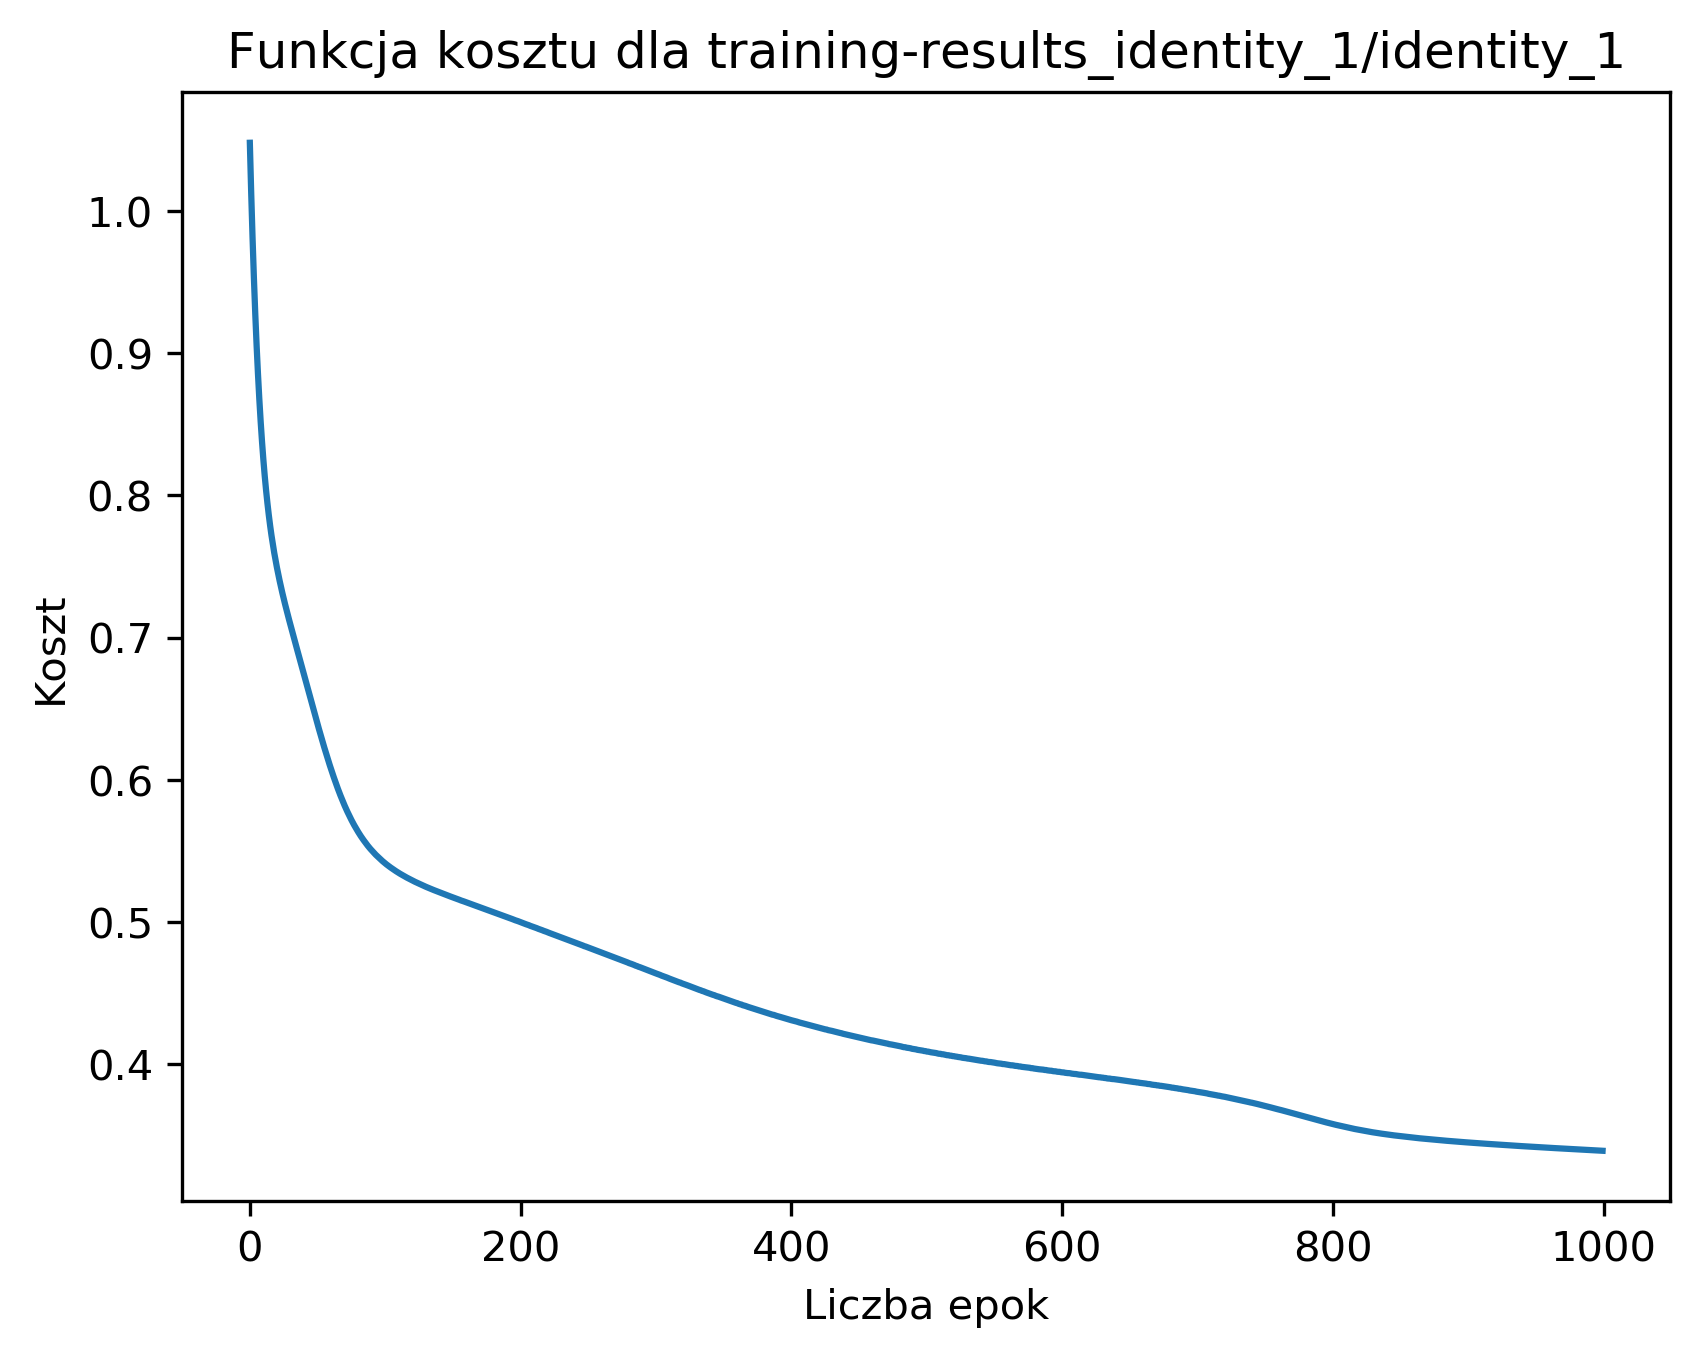
\includegraphics[width=110mm]{wykresy/identity_1_cost.png}
                \caption{wsp. nauki=0.6 , wsp. momentum=0.0, bez biasu}
            \end{figure}
            \begin{figure}[!htbp]
                \centering
                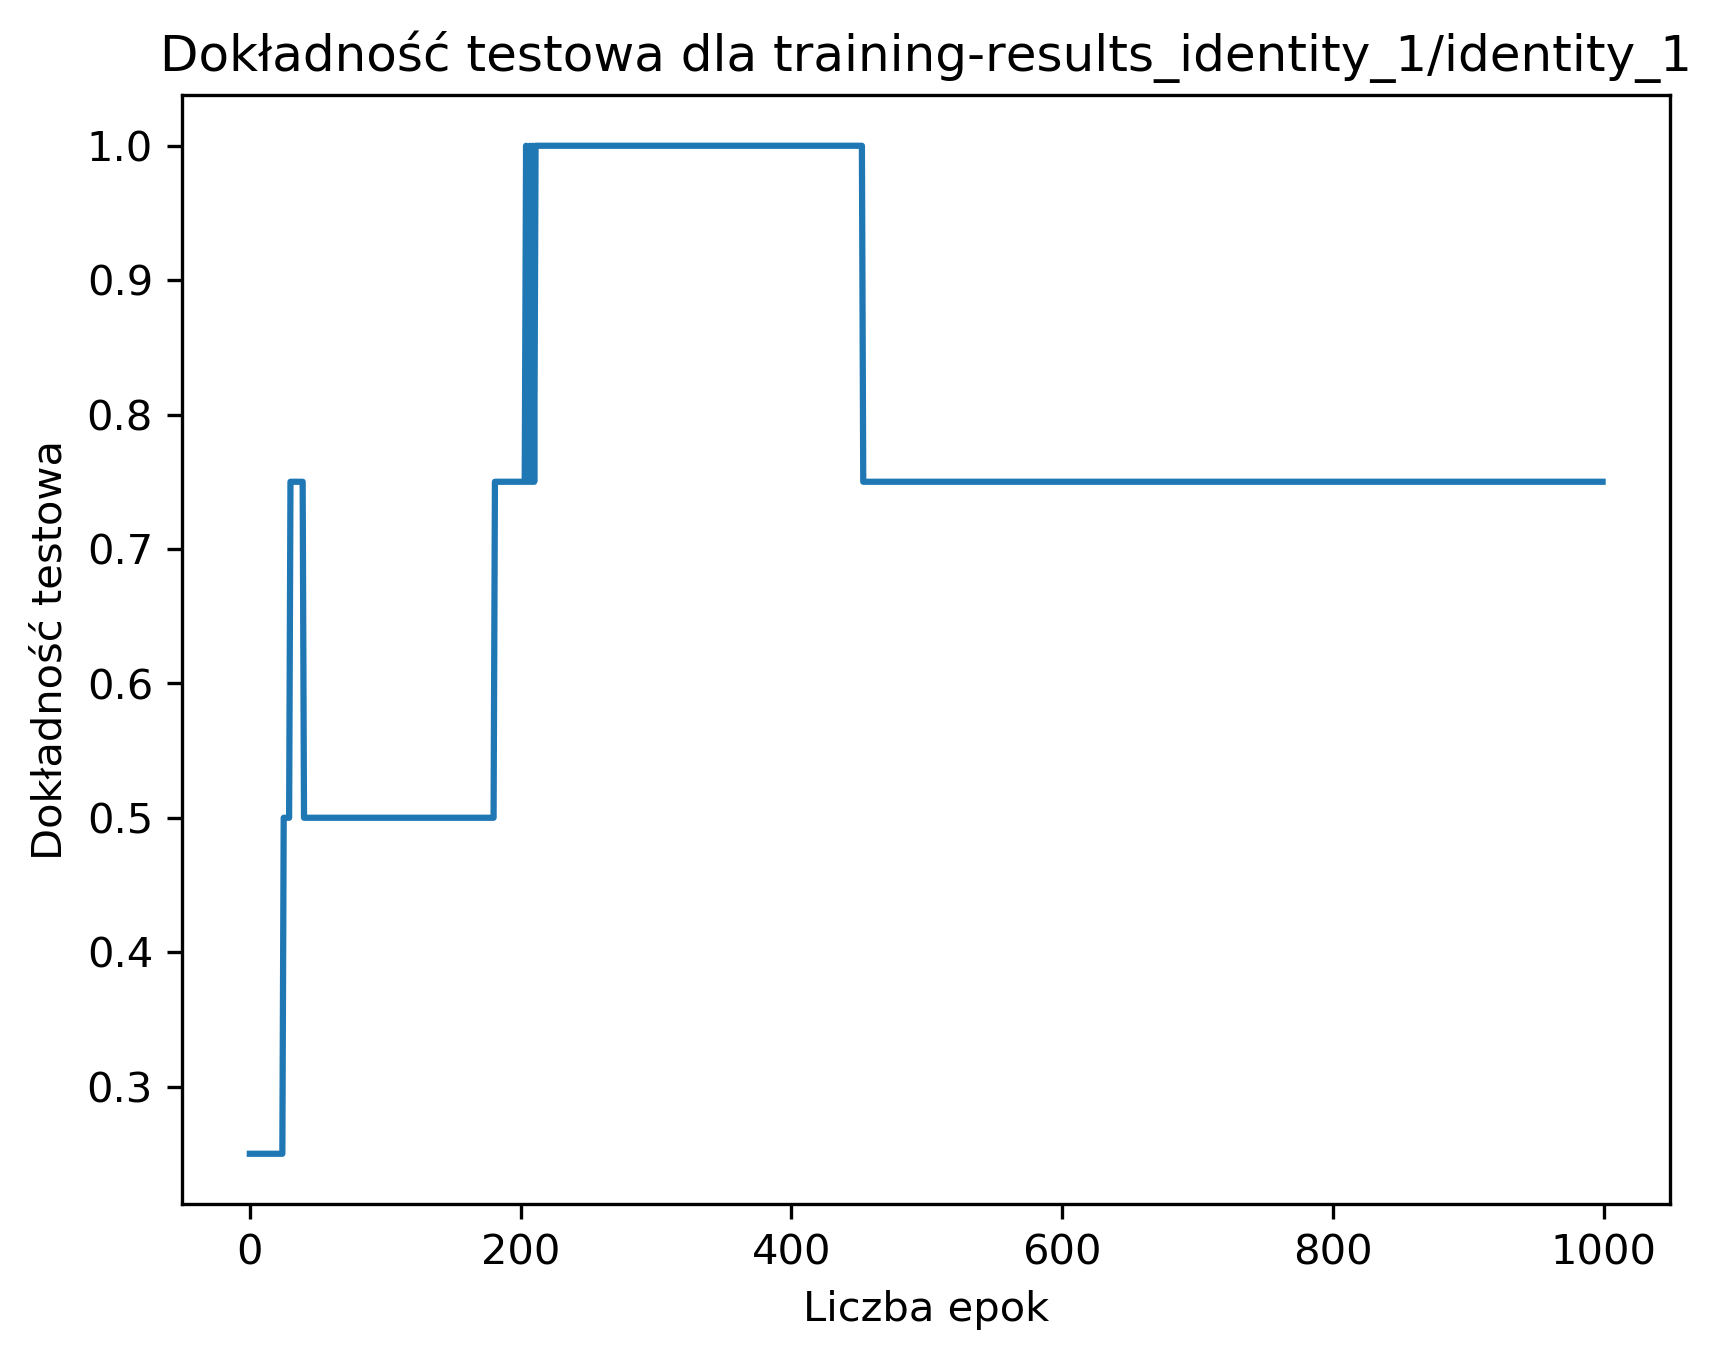
\includegraphics[width=110mm]{wykresy/identity_1_testing-accuracy.png}
                \caption{wsp. nauki=0.6 , wsp. momentum=0.0, bez biasu}
            \end{figure}
            \FloatBarrier
        %---------------------------------------------------%
            \begin{figure}[!htbp]
                \centering
                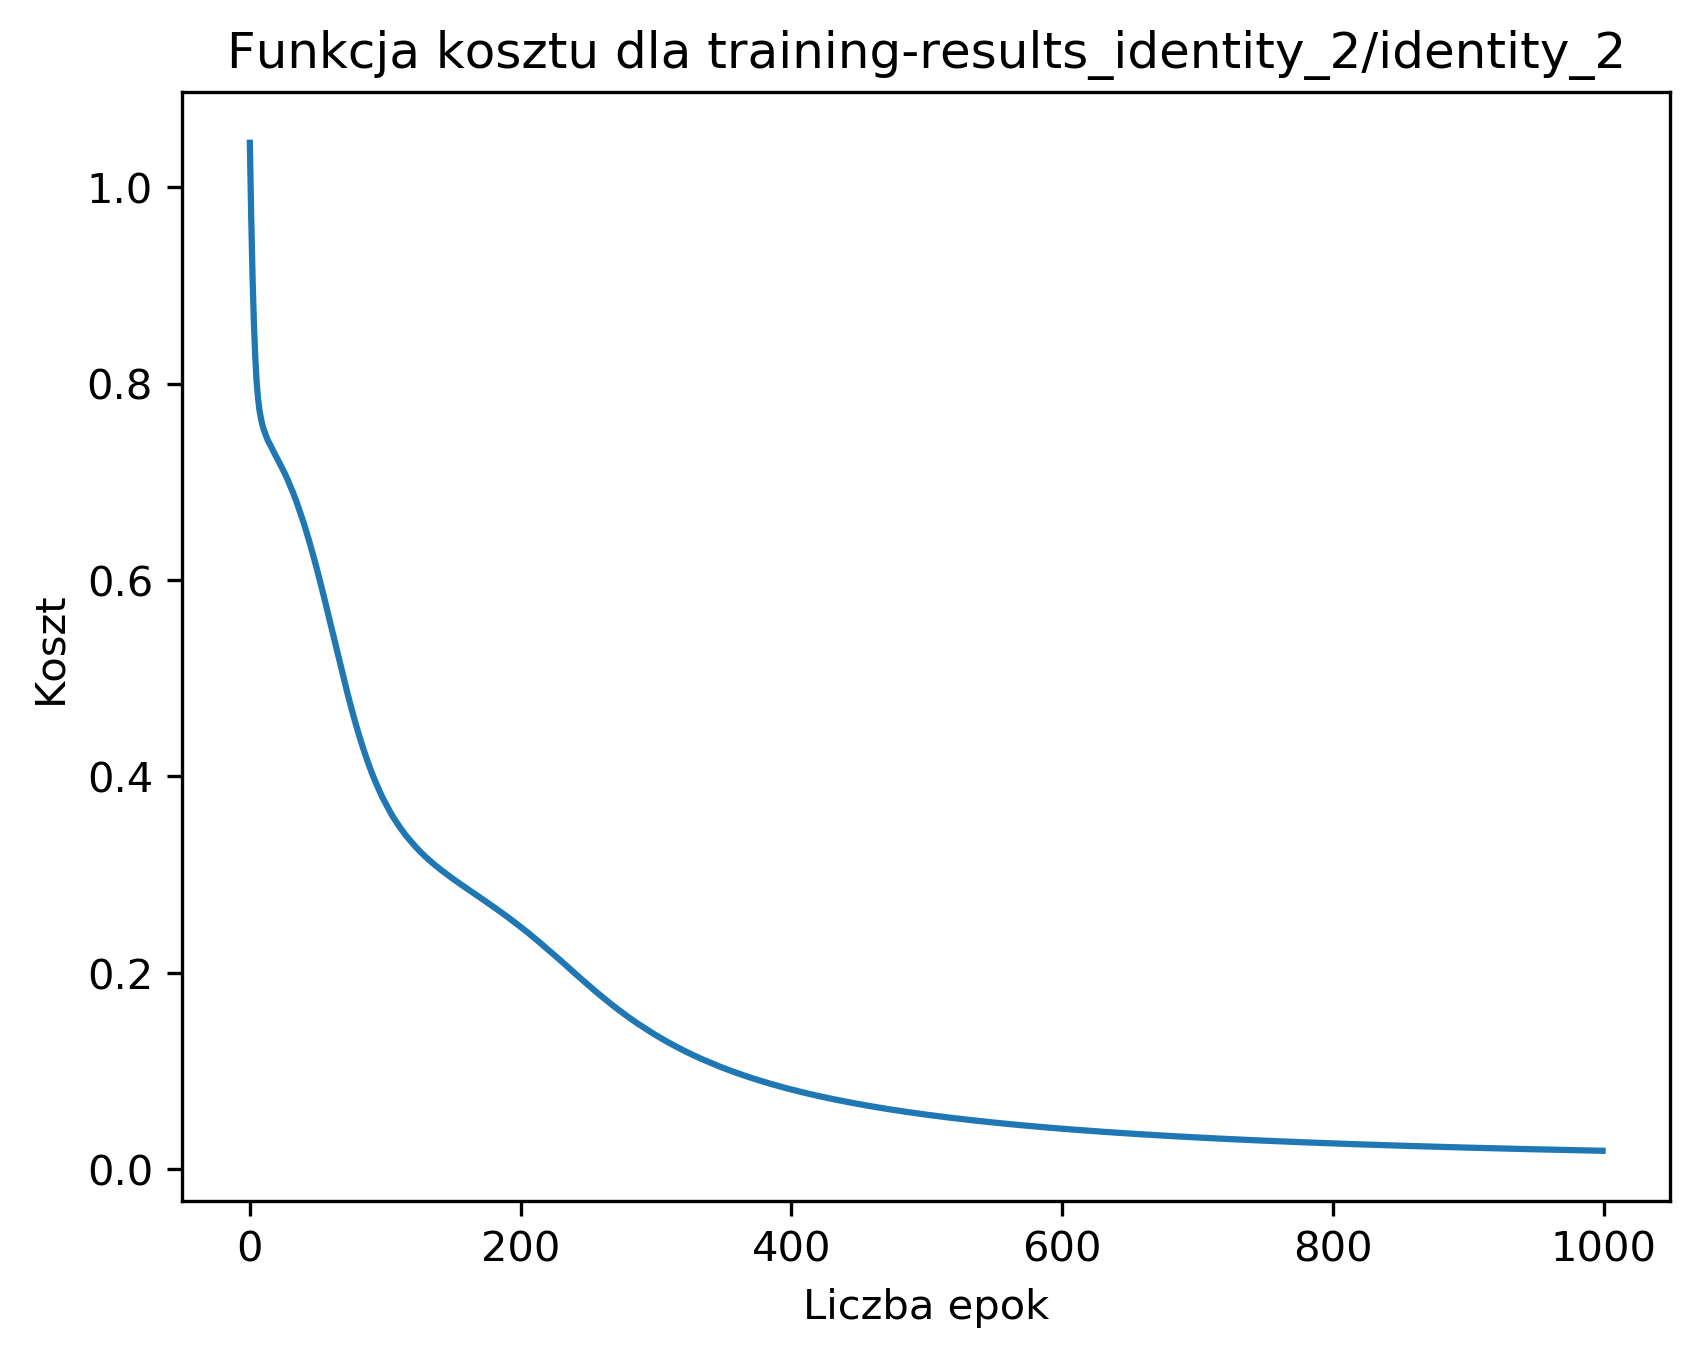
\includegraphics[width=110mm]{wykresy/identity_2_cost.png}
                \caption{wsp. nauki=0.6 , wsp. momentum=0.0, z biasem}
            \end{figure}
            \begin{figure}[!htbp]
                \centering
                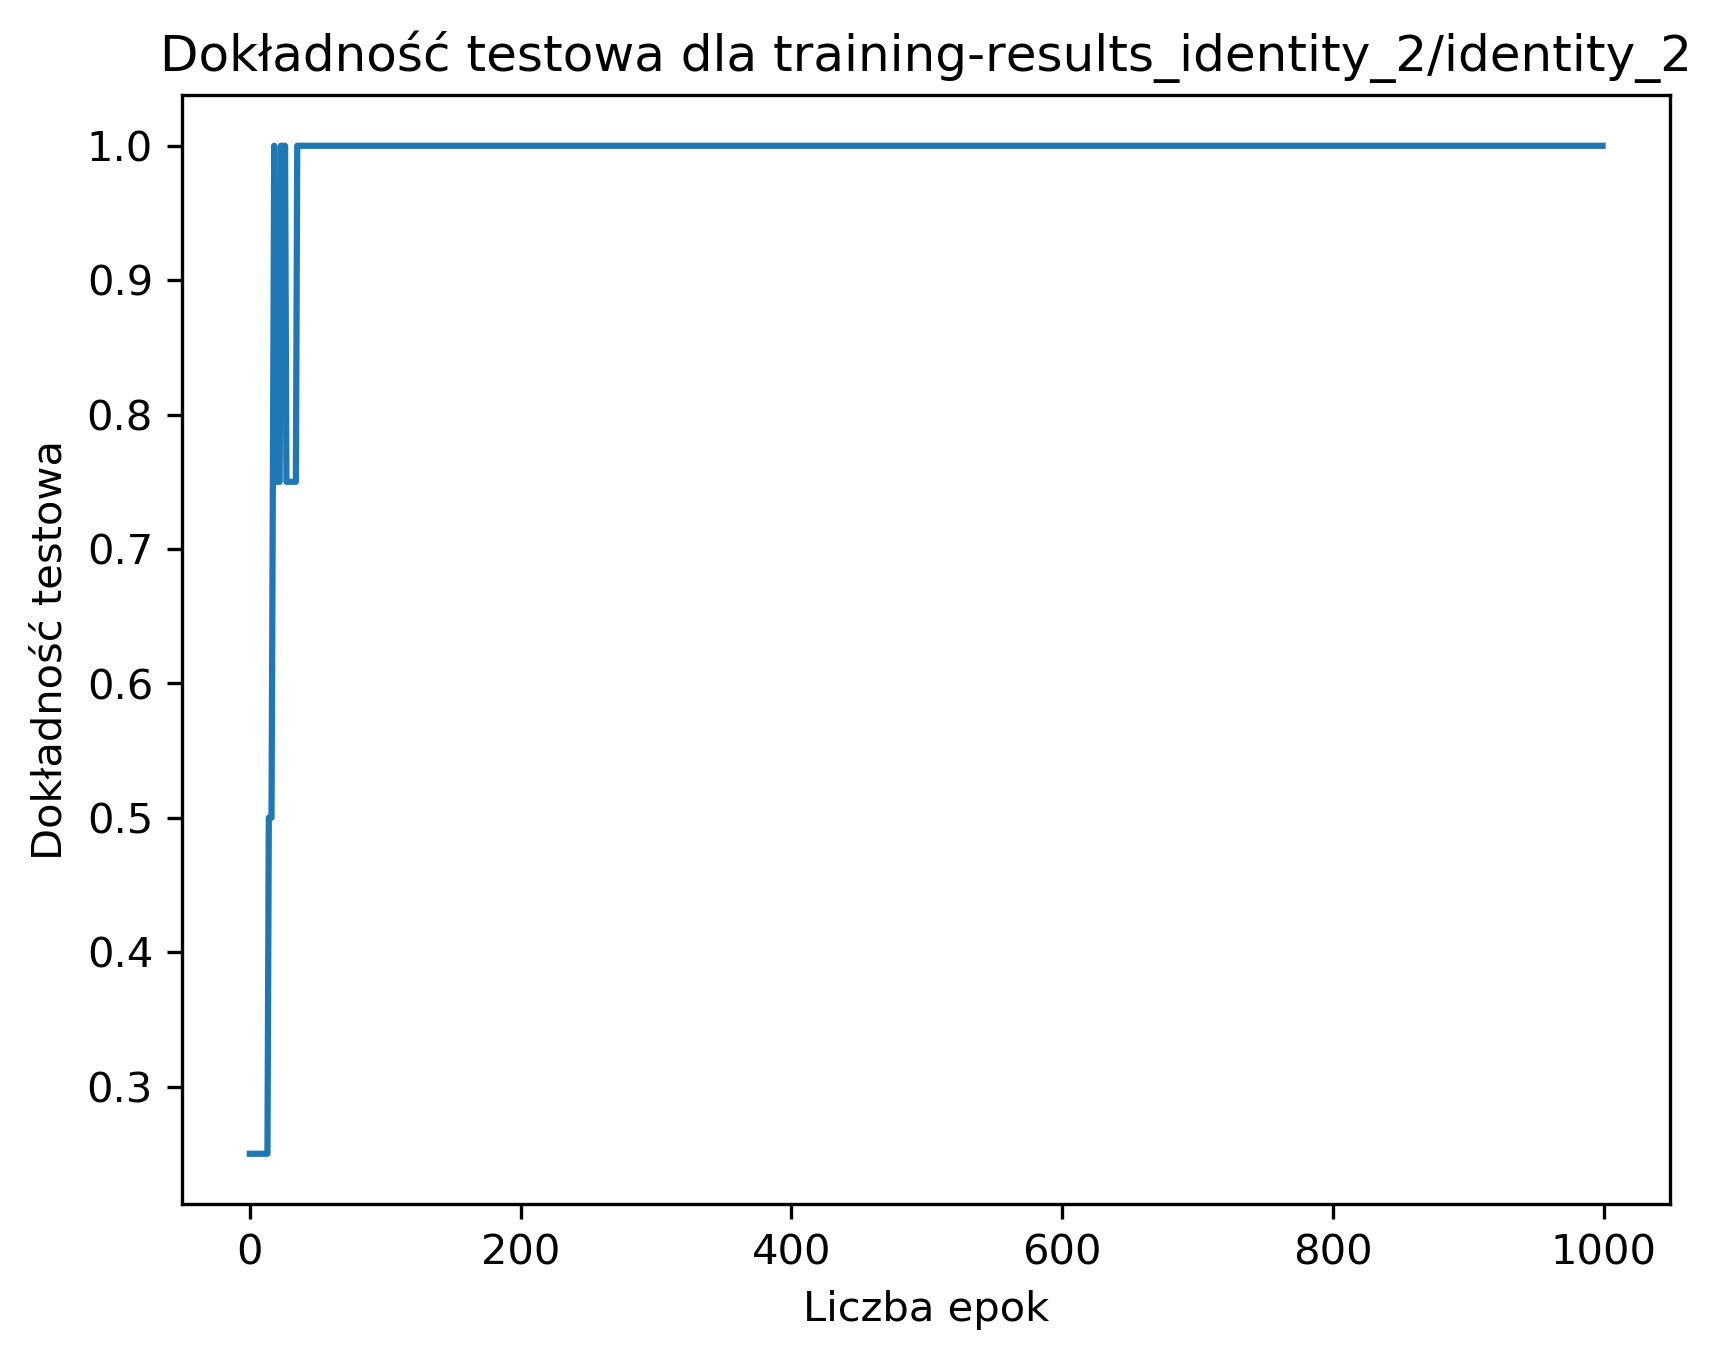
\includegraphics[width=110mm]{wykresy/identity_2_testing-accuracy.png}
                \caption{wsp. nauki=0.6 , wsp. momentum=0.0, z biasem}
            \end{figure}
            \FloatBarrier
        %---------------------------------------------------%
            \begin{figure}[!htbp]
                \centering
                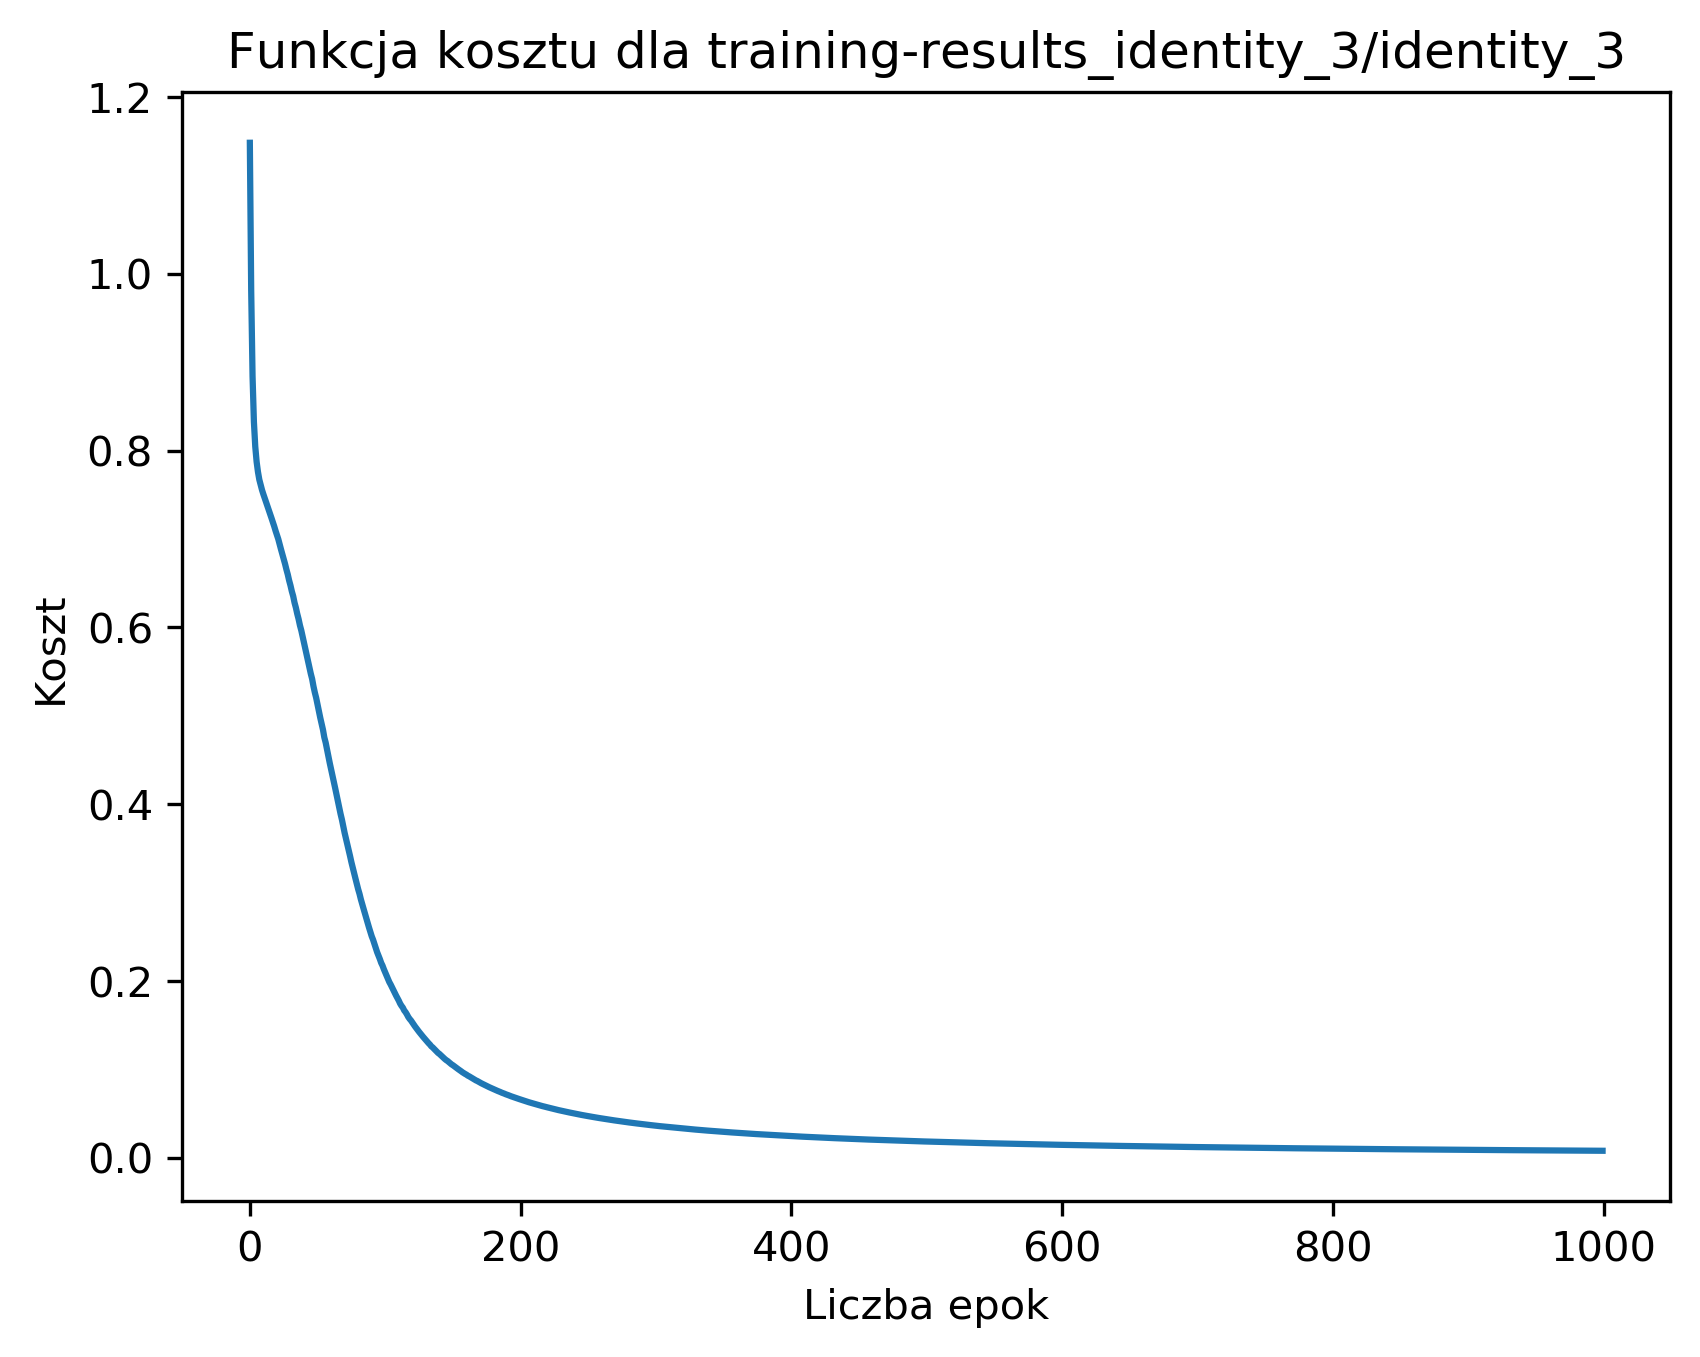
\includegraphics[width=110mm]{wykresy/identity_3_cost.png}
                \caption{wsp. nauki=0.9 , wsp. momentum=0.0, z biasem}
            \end{figure}
            \begin{figure}[!htbp]
                \centering
                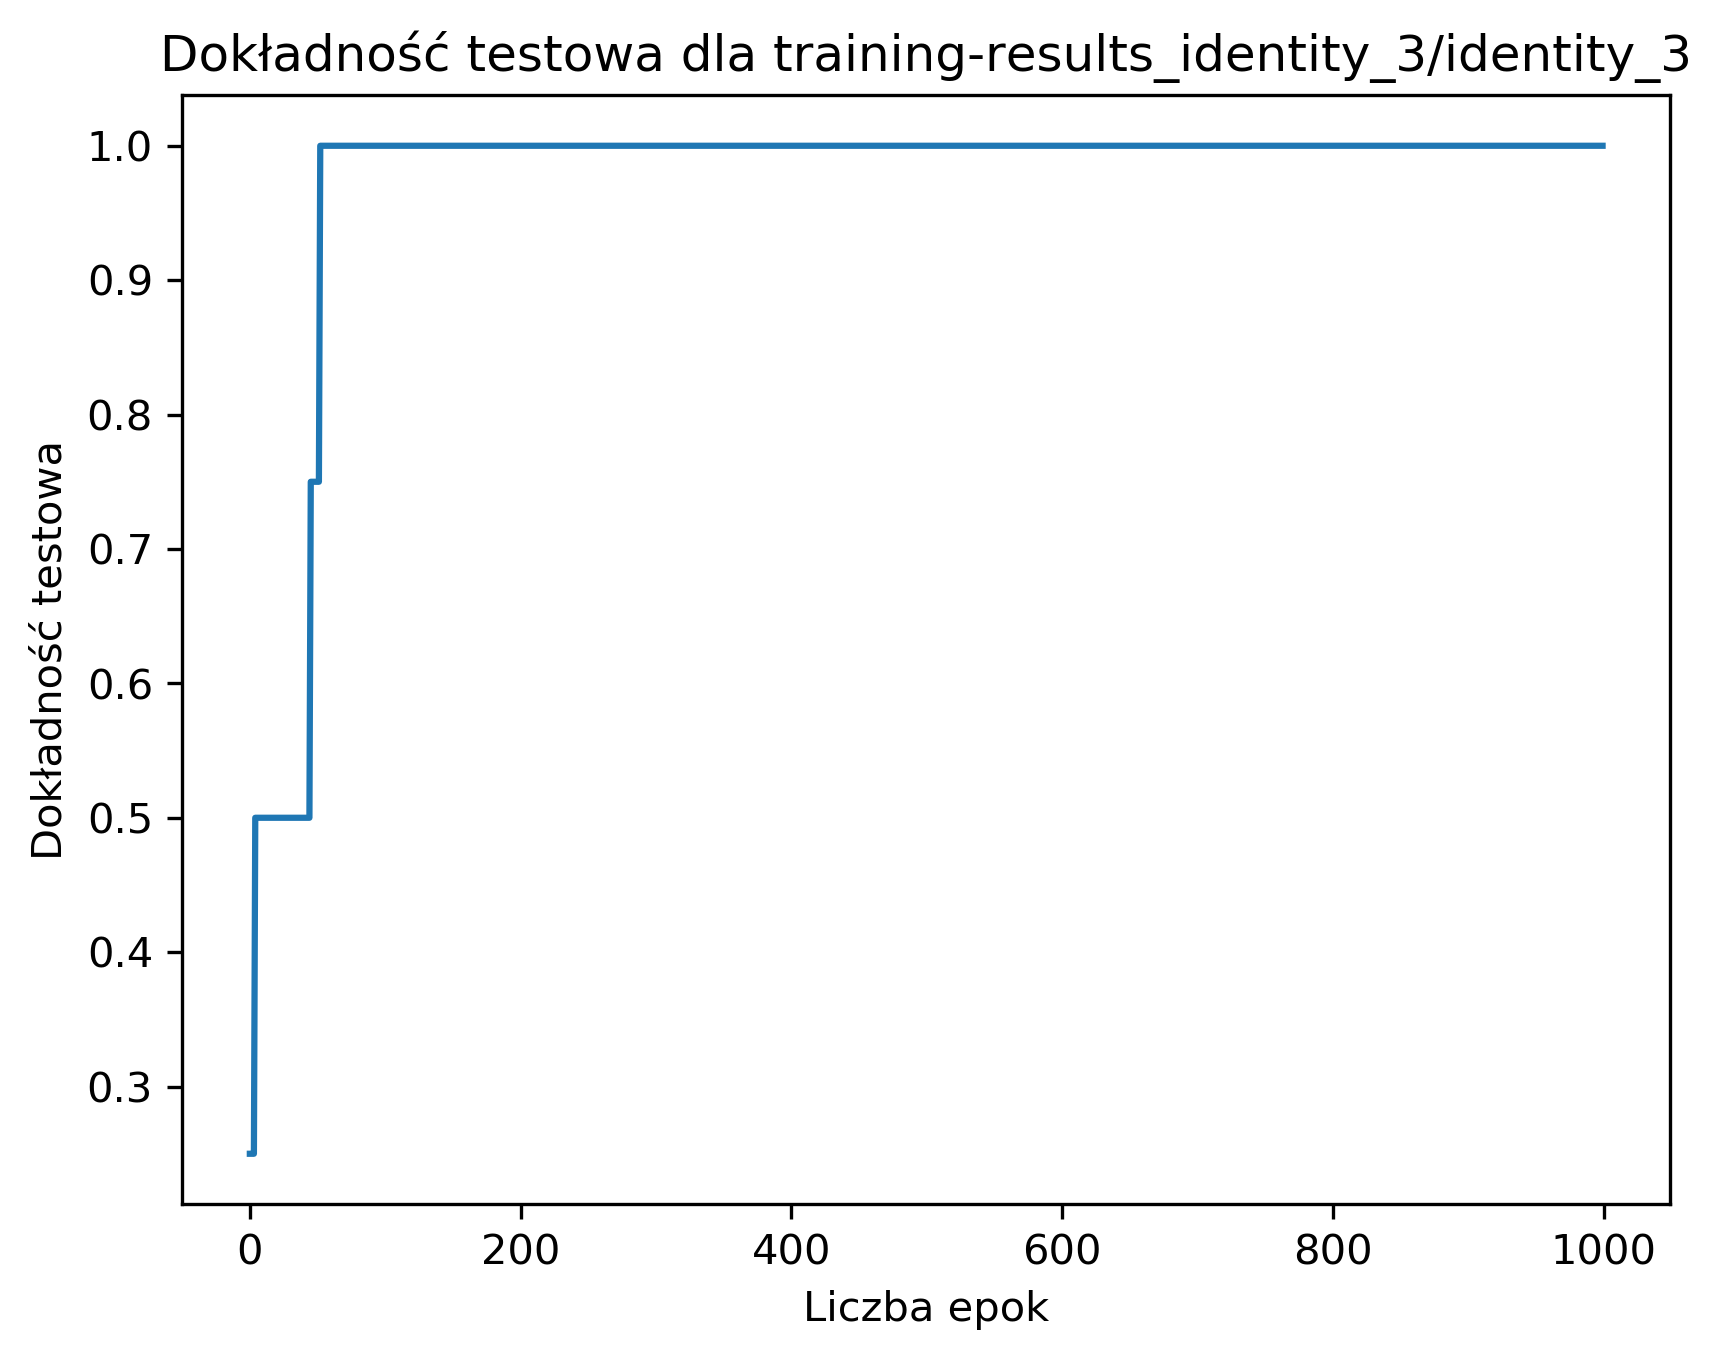
\includegraphics[width=110mm]{wykresy/identity_3_testing-accuracy.png}
                \caption{wsp. nauki=0.9 , wsp. momentum=0.0, z biasem}
            \end{figure}
            \FloatBarrier
        %---------------------------------------------------%
            \begin{figure}[!htbp]
                \centering
                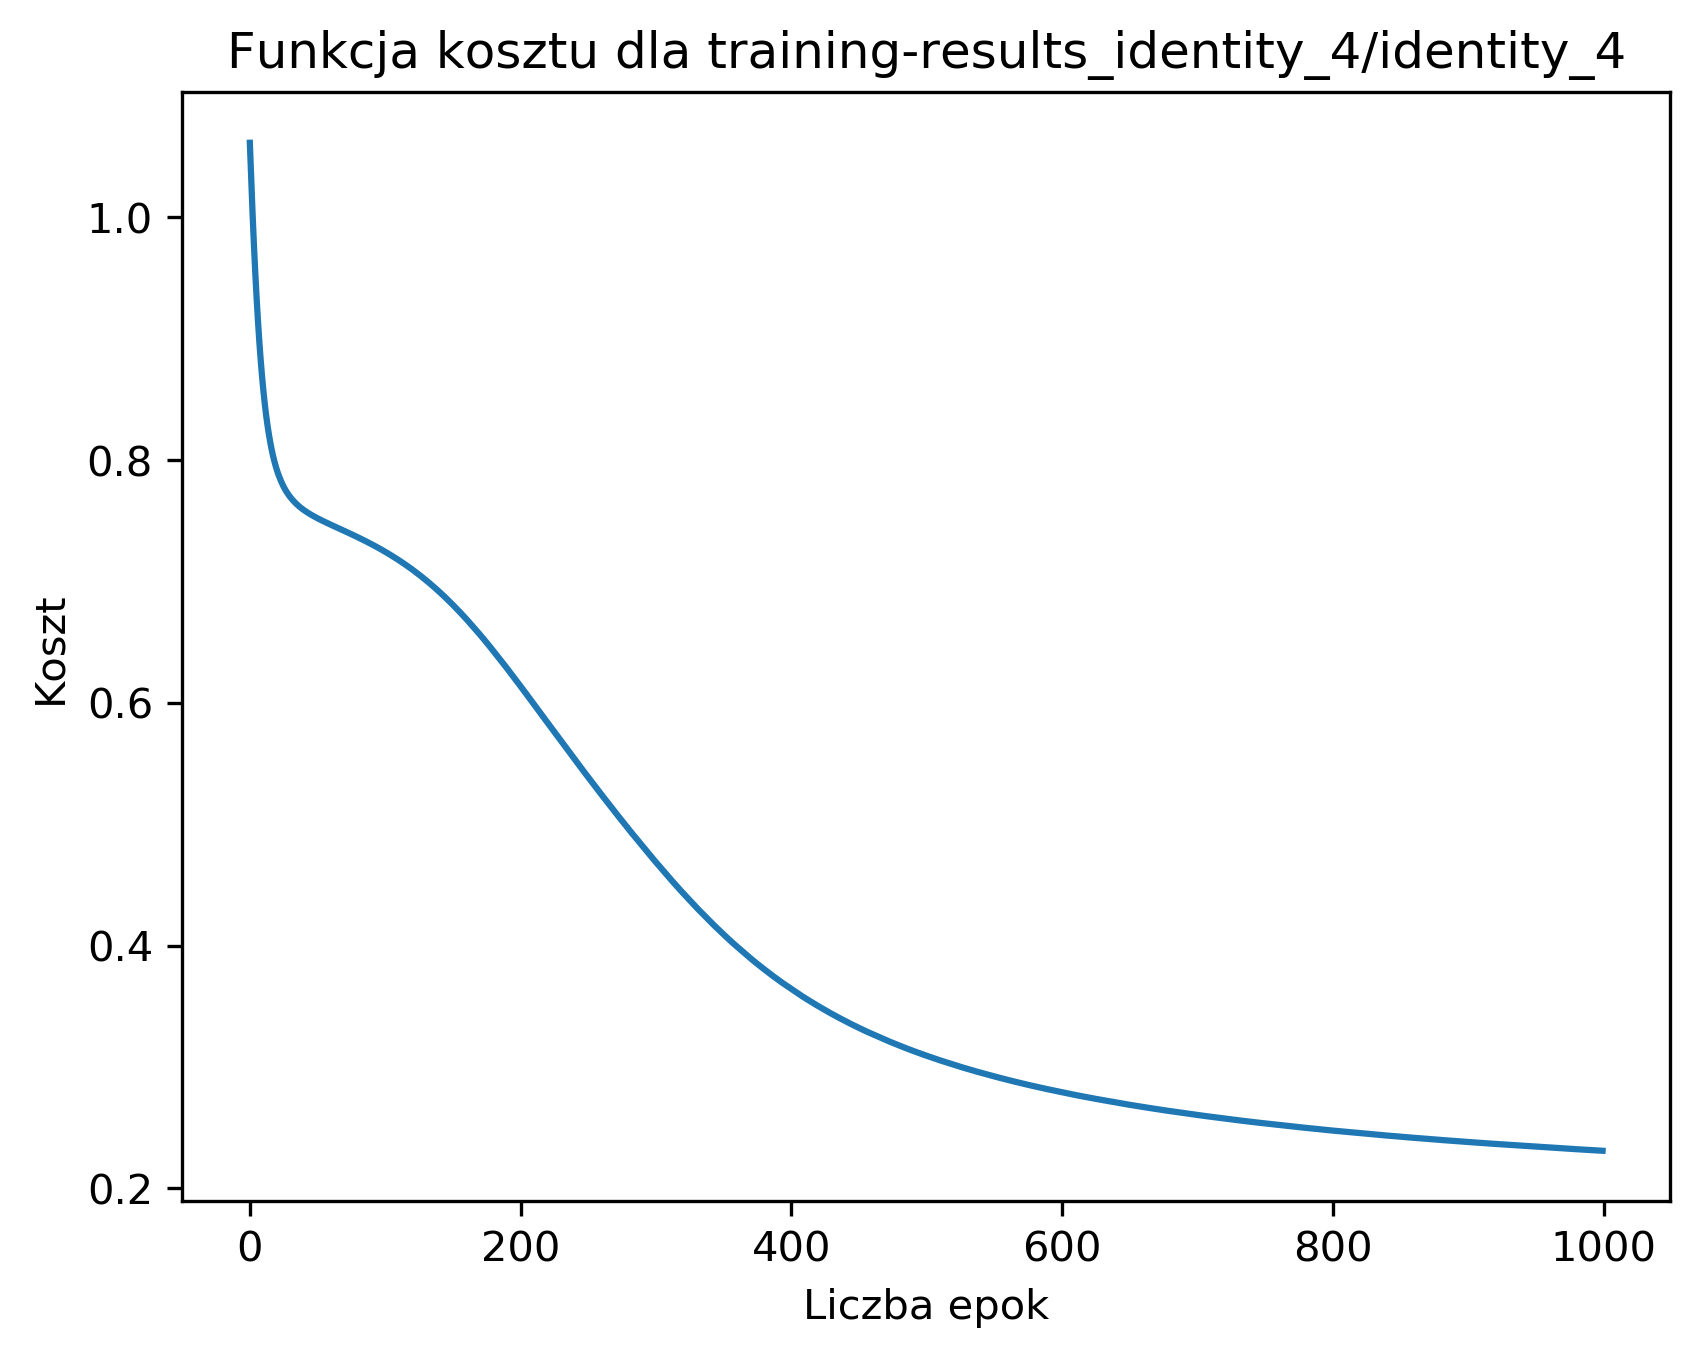
\includegraphics[width=110mm]{wykresy/identity_4_cost.png}
                \caption{wsp. nauki=0.2 , wsp. momentum=0.0, z biasem}
            \end{figure}
            \begin{figure}[!htbp]
                \centering
                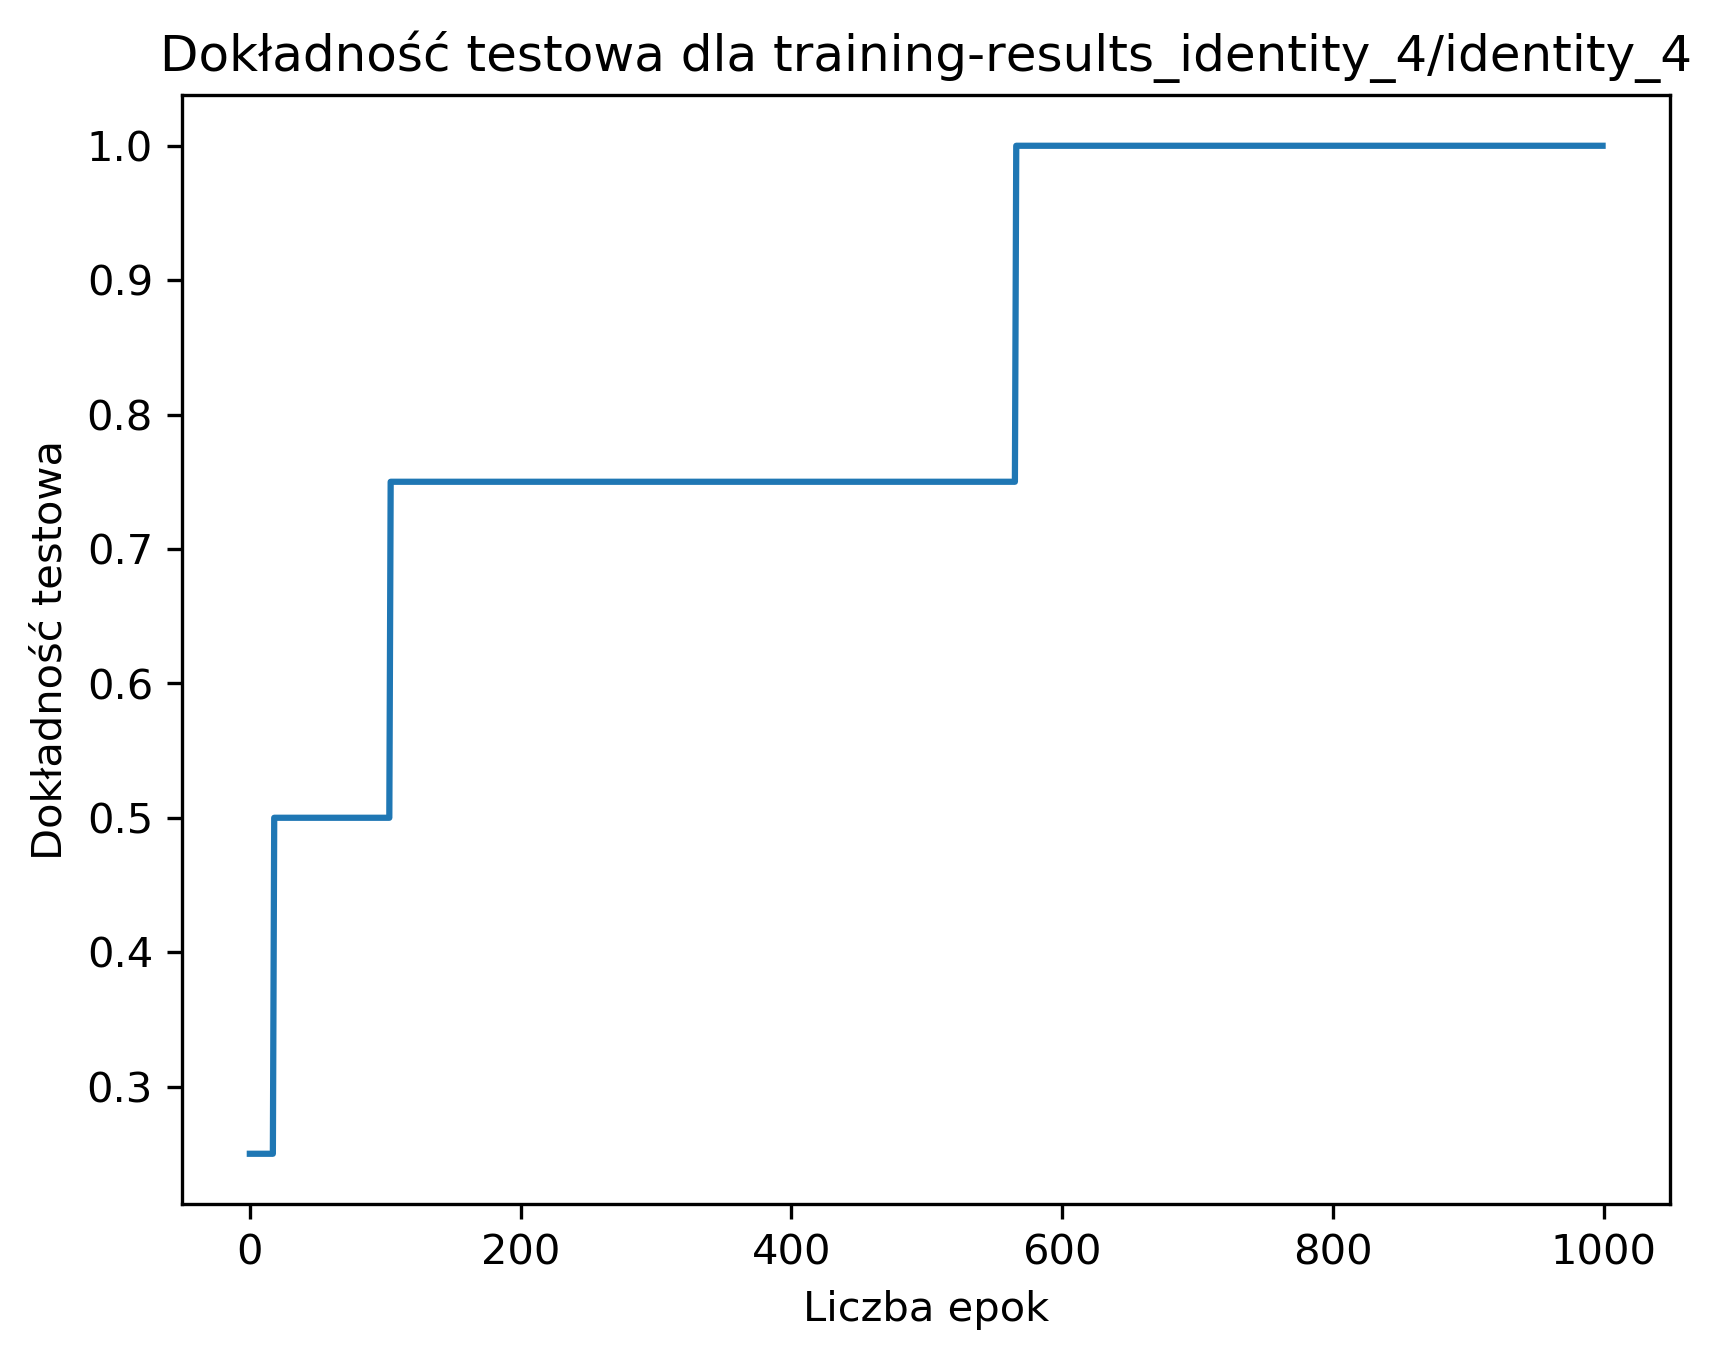
\includegraphics[width=110mm]{wykresy/identity_4_testing-accuracy.png}
                \caption{wsp. nauki=0.2 , wsp. momentum=0.0, z biasem}
            \end{figure}
            \FloatBarrier
        %---------------------------------------------------%
            \begin{figure}[!htbp]
                \centering
                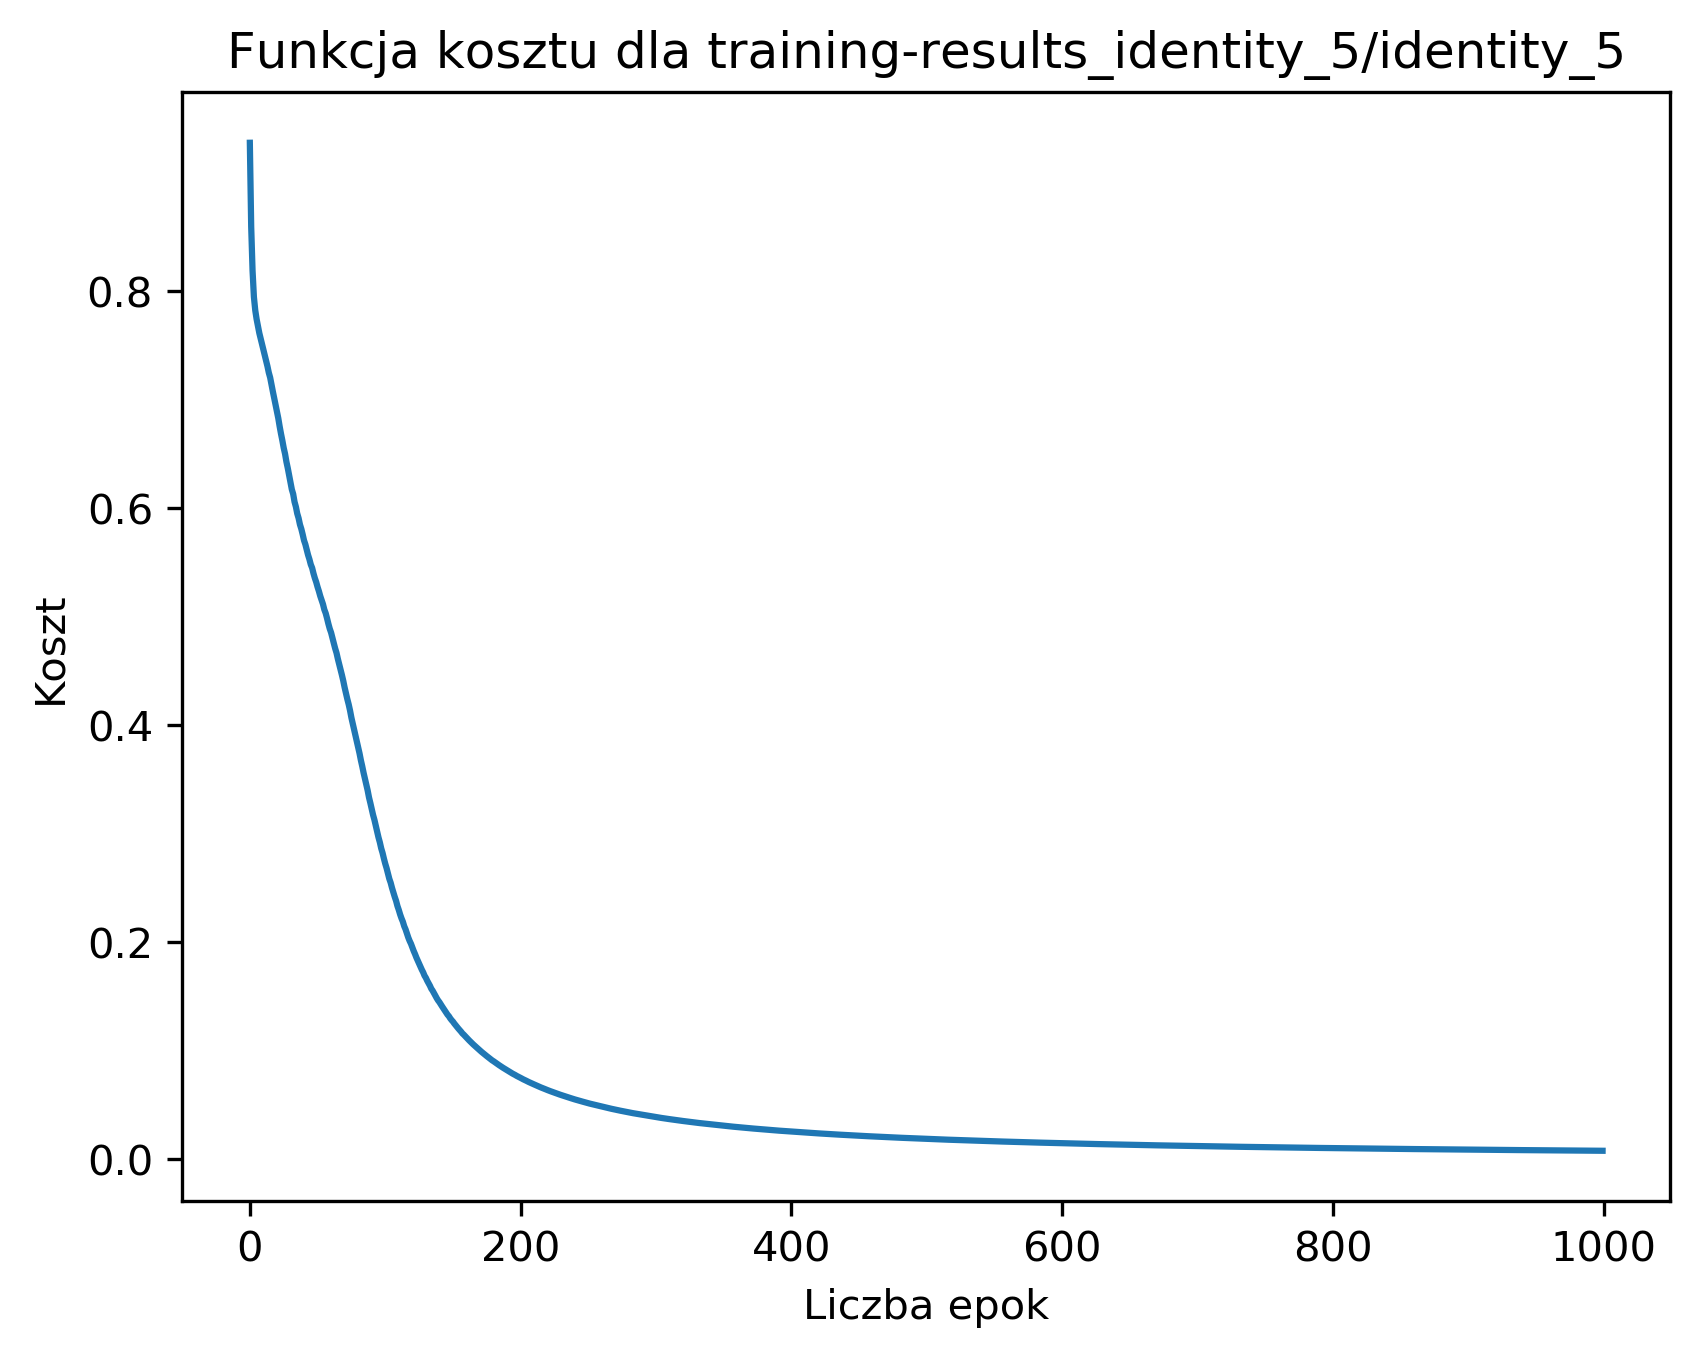
\includegraphics[width=110mm]{wykresy/identity_5_cost.png}
                \caption{wsp. nauki=0.9 , wsp. momentum=0.6, z biasem}
            \end{figure}
            \begin{figure}[!htbp]
                \centering
                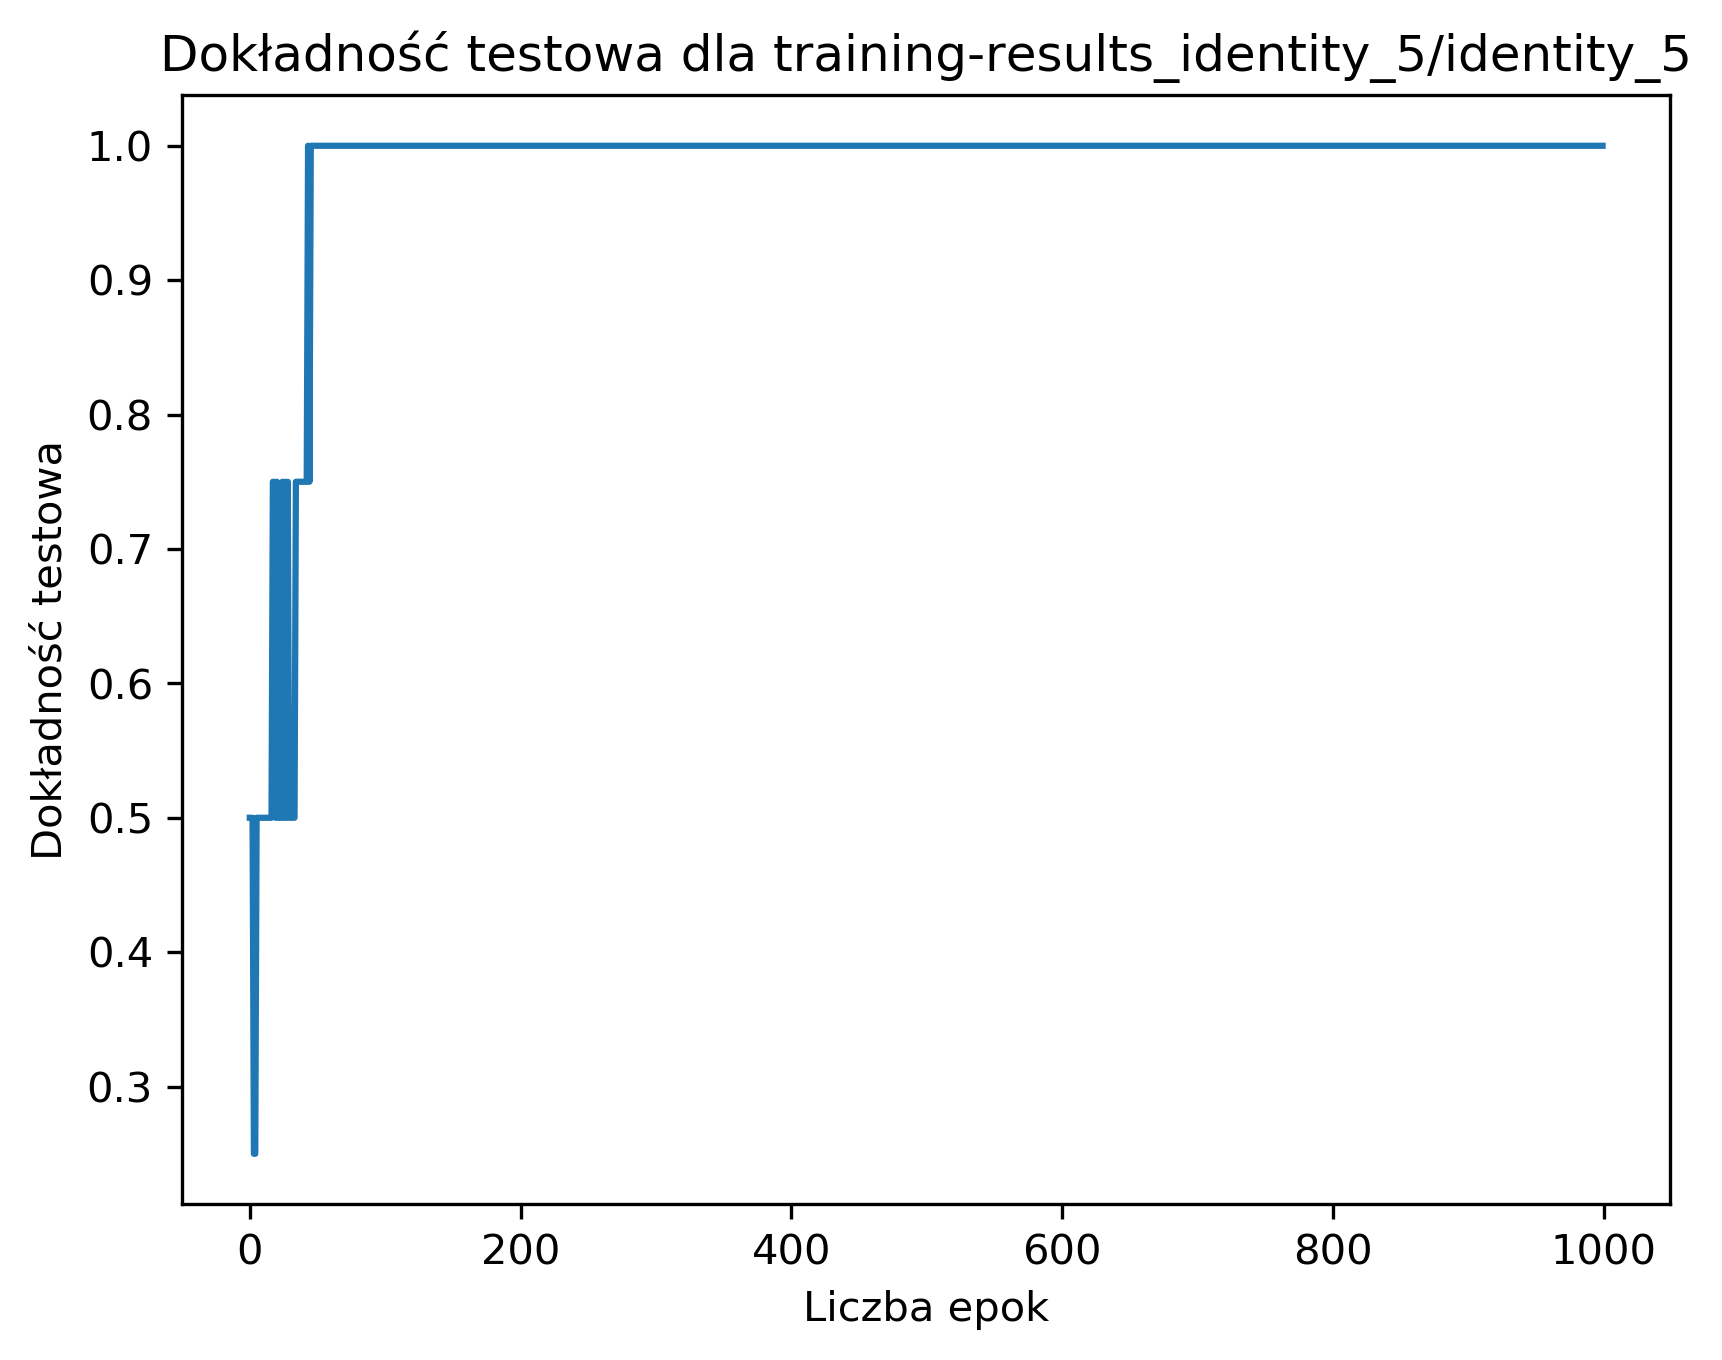
\includegraphics[width=110mm]{wykresy/identity_5_testing-accuracy.png}
                \caption{wsp. nauki=0.9 , wsp. momentum=0.6, z biasem}
            \end{figure}
            \FloatBarrier
        %---------------------------------------------------%
            \begin{figure}[!htbp]
                \centering
                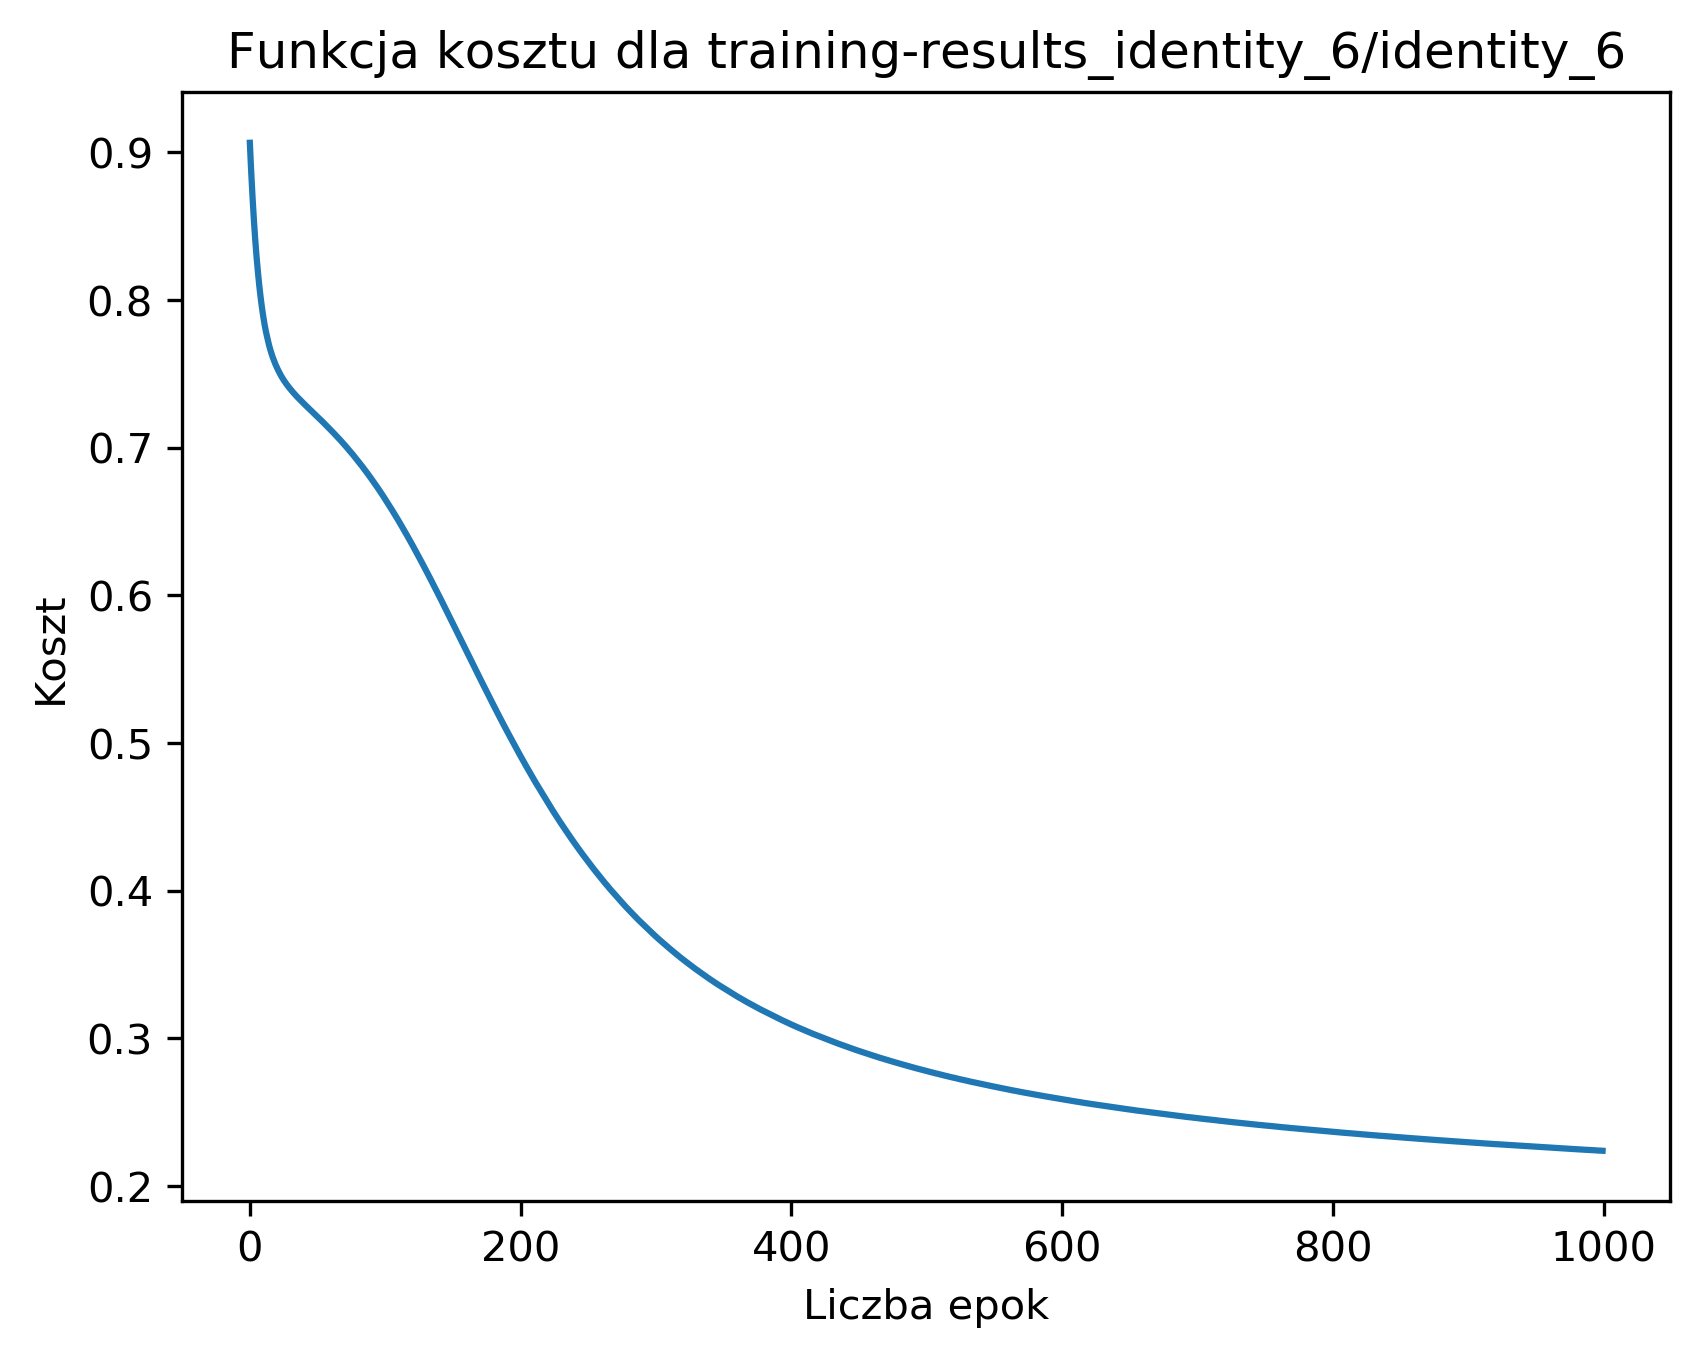
\includegraphics[width=110mm]{wykresy/identity_6_cost.png}
                \caption{wsp. nauki=0.2 , wsp. momentum=0.9, z biasem}
            \end{figure}
            \begin{figure}[!htbp]
                \centering
                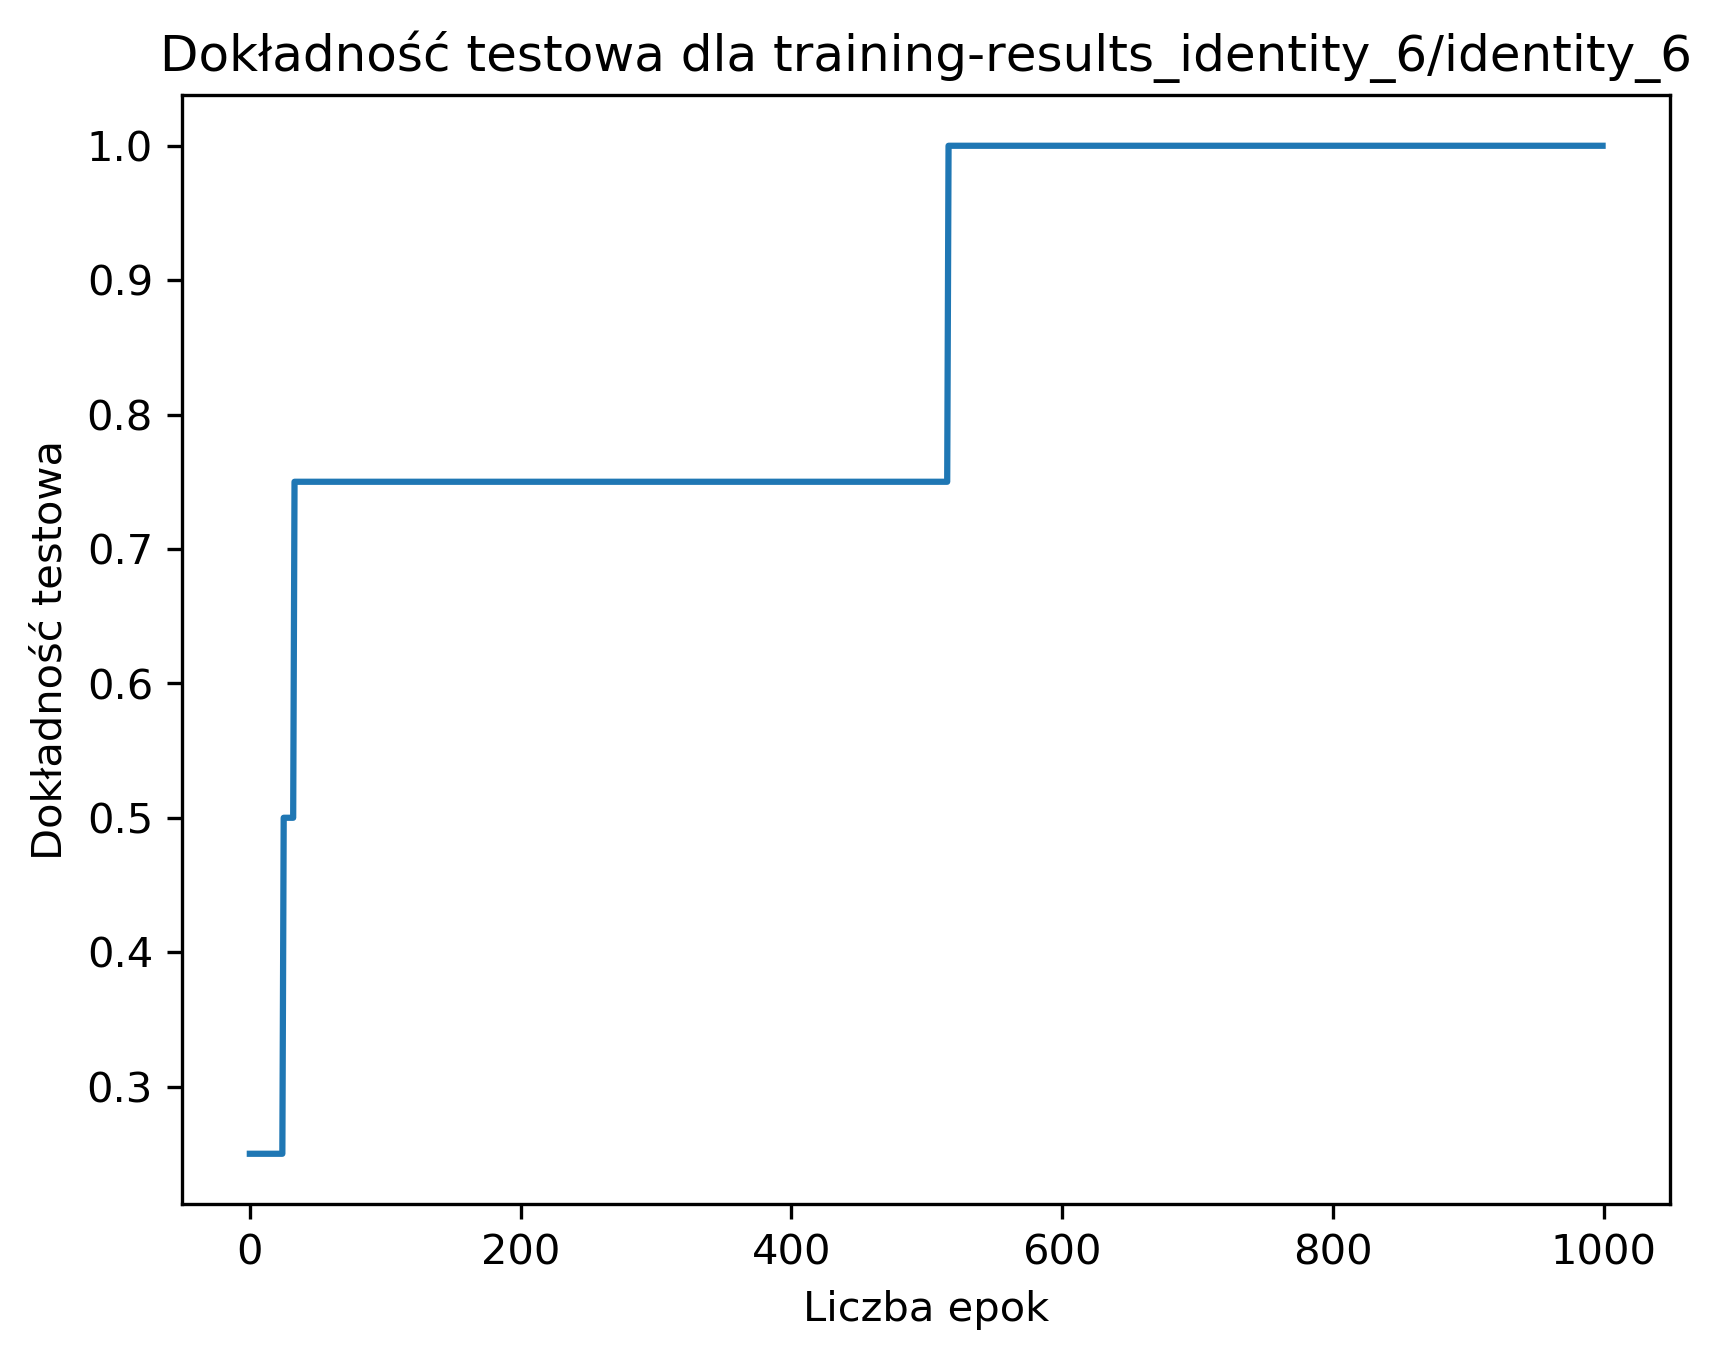
\includegraphics[width=110mm]{wykresy/identity_6_testing-accuracy.png}
                \caption{wsp. nauki=0.2 , wsp. momentum=0.9, z biasem}
            \end{figure}
            \FloatBarrier
        %---------------------------------------------------%
        }
    %---------------------------------------------------%
        \subsection{Zbior irysów}
        {
            \subsubsection{Perceptron wielowarstwowy}
            {
                Wybrane parametry to: neurony ukryte - 2, liczba epok - 1000, docelowa dokł. funkcji kosztu: 0.01,
                współczynnik nauki początkowy: 0.1, współczynnik nauki końcowy: 0.05, momentum: 0.5

                \begin{figure}[!htbp]
                    \centering
                    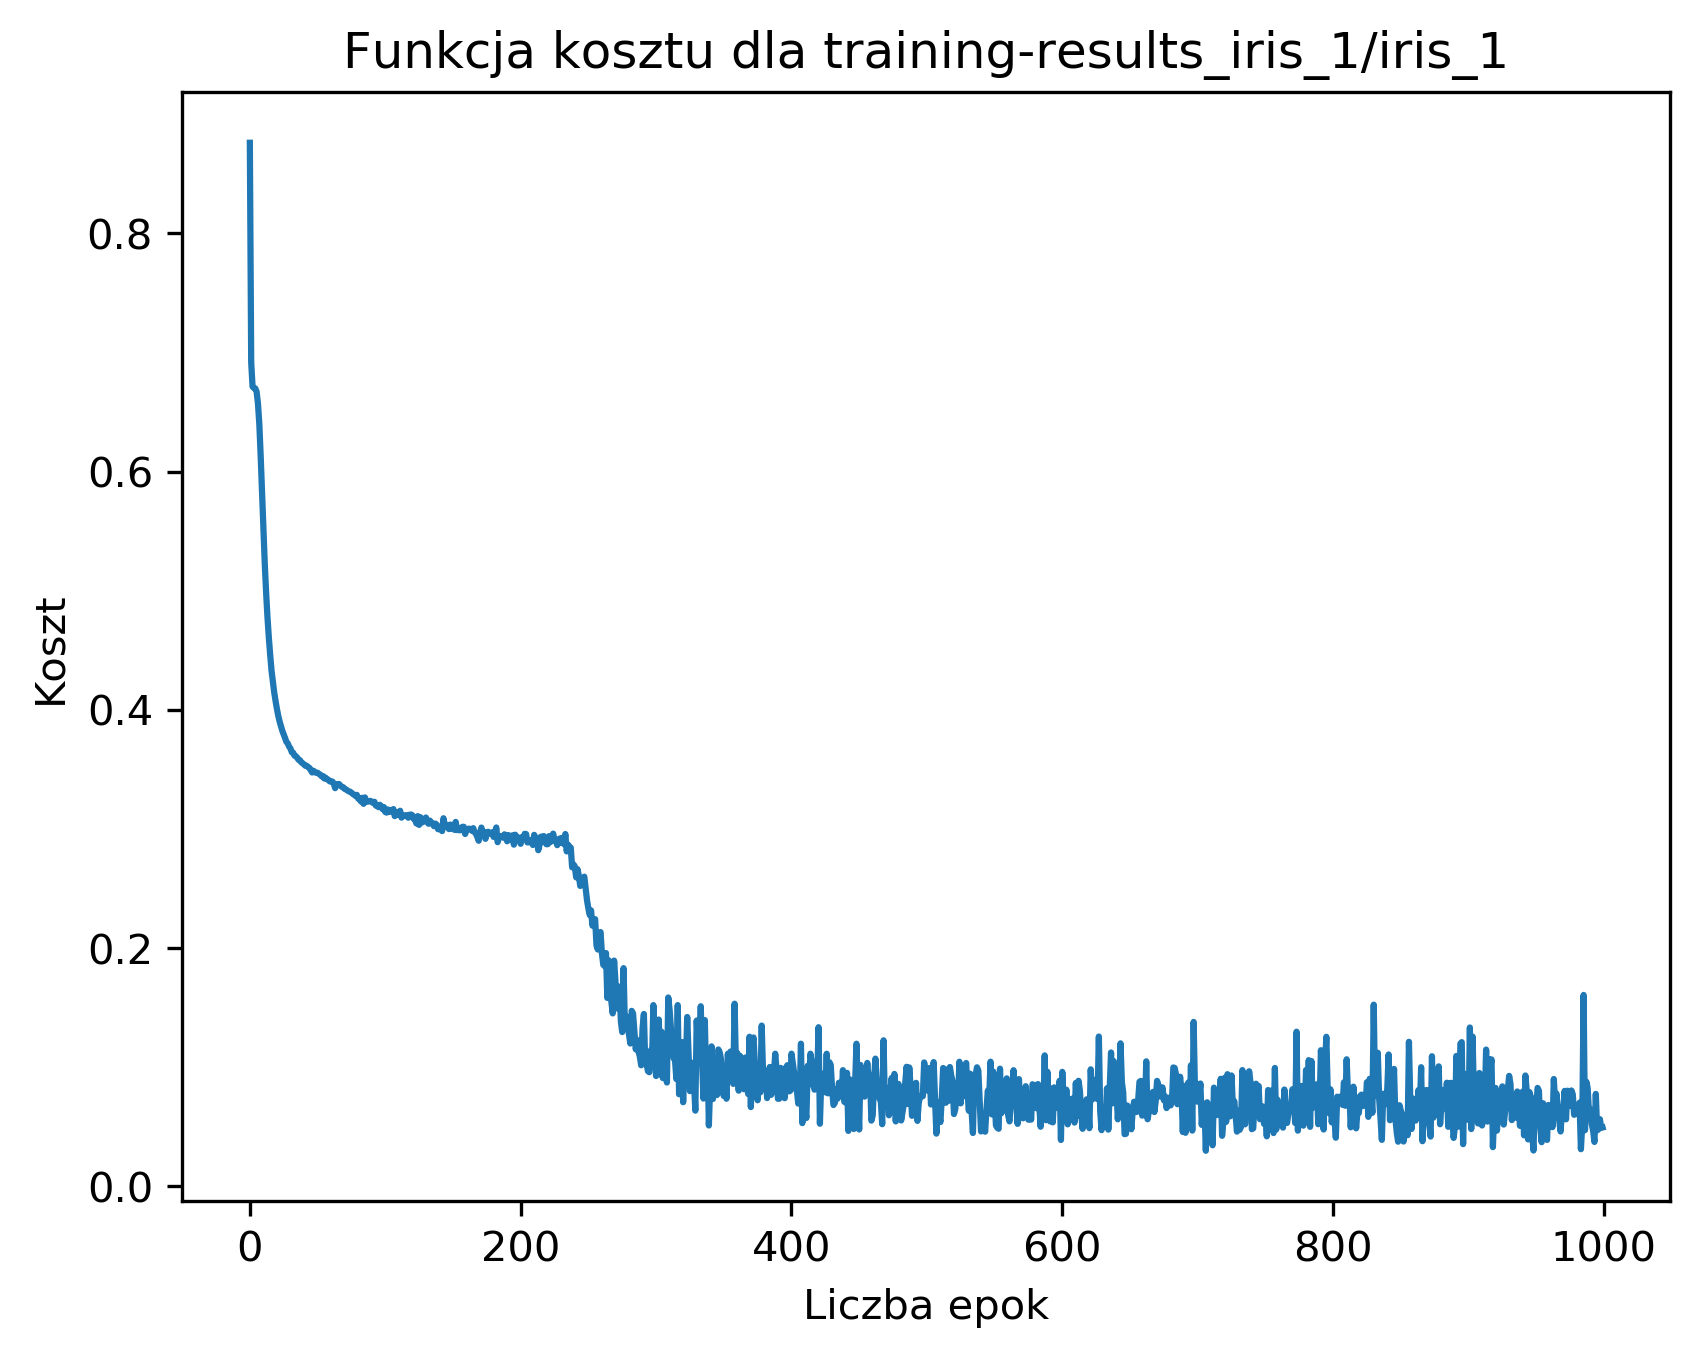
\includegraphics[width=110mm]{wykresy/iris_1_cost.png}
                    \caption{Tryb z domyślnymi danymi}
                \end{figure}
                \begin{figure}[!htbp]
                    \centering
                    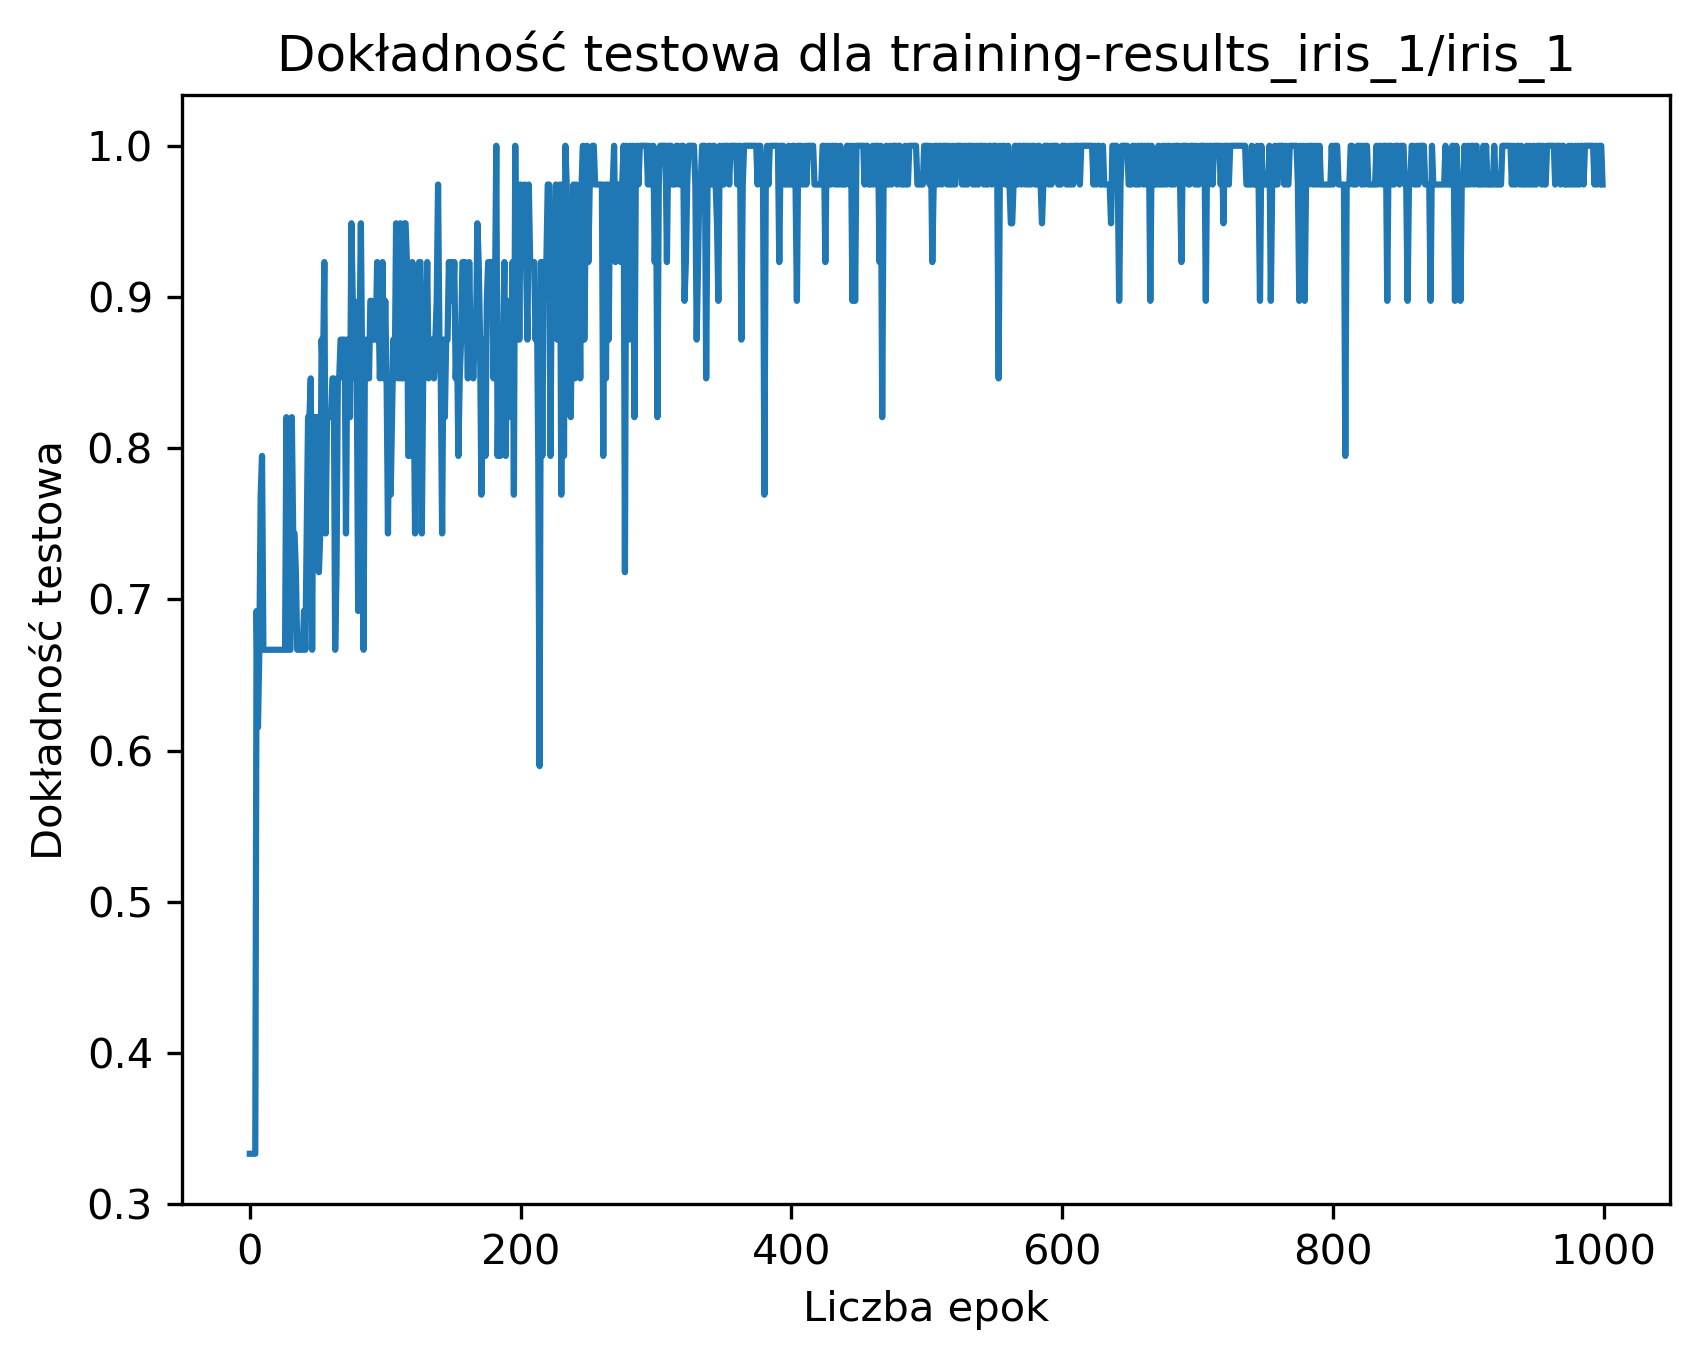
\includegraphics[width=110mm]{wykresy/iris_1_testing-accuracy.png}
                    \caption{Tryb z domyślnymi danymi}
                \end{figure}
                \begin{figure}[!htbp]
                    \centering
                    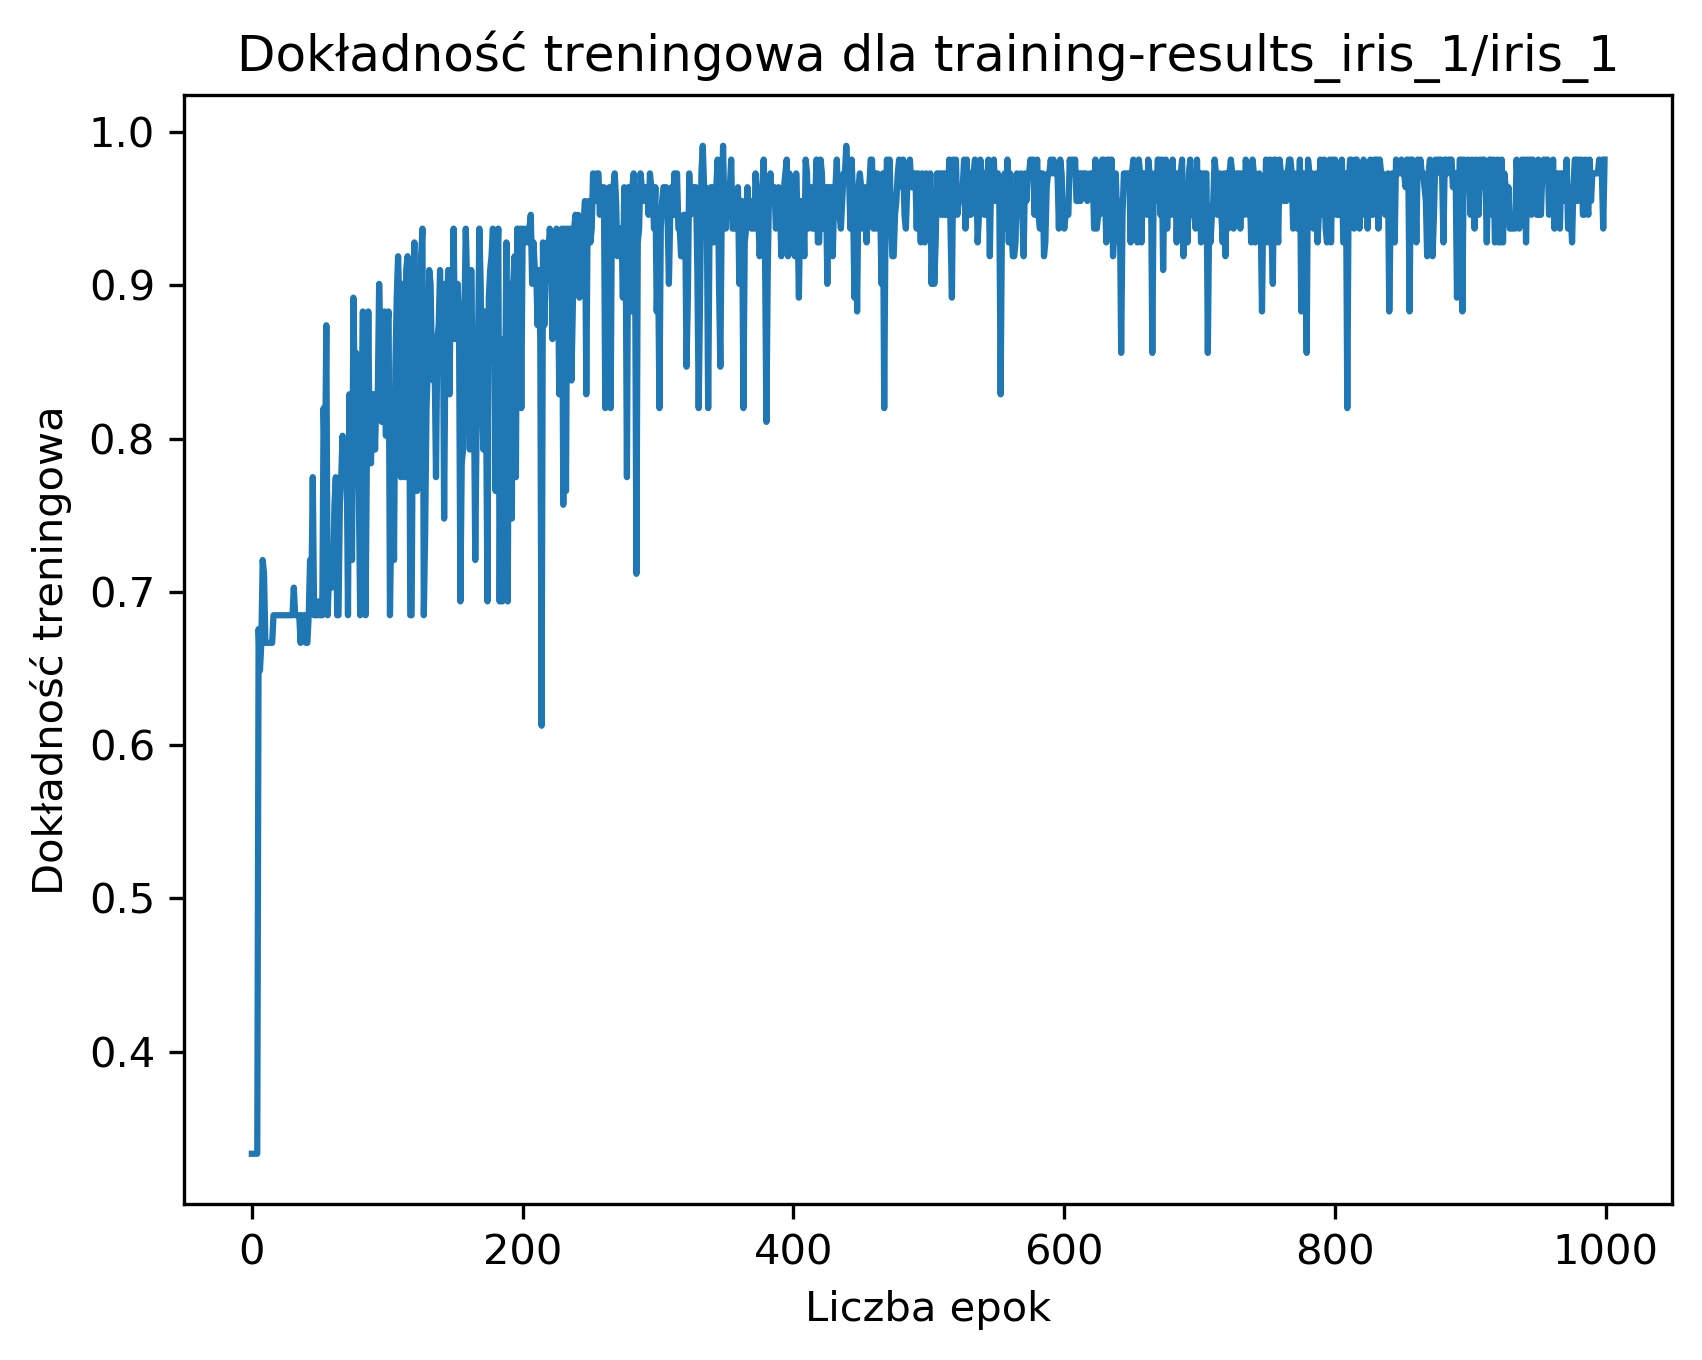
\includegraphics[width=110mm]{wykresy/iris_1_training-accuracy.png}
                    \caption{Tryb z domyślnymi danymi}
                \end{figure}
                \FloatBarrier
            %---------------------------------------------------%
                \textbf{Tablice pomyłem}
                \begin{lstlisting}
>> ./data/iris-train.csv

> Global confusion matrix:
                [Iris-setosa][Iris-versicolor][Iris-virginica]
                [Iris-setosa]       37 0 0
                [Iris-versicolor]        0 35 0
                [Iris-virginica]        0 2 37


                Total population | 111

                Accuracy | 98.1982 %



                > [Iris-setosa]
                [Positive]    [Negative]
                [Positive]           37 0
                [Negative]            0 74


                Total population | 111

                True positive | 37
                True negative | 74
                False positive (type I error) | 0
                False negative (type II error) | 0

                Predicted positive | 37
                Predicted negative | 74
                Actual positive | 37
                Actual negative | 74

                Positive predictive value | 100 %
                False discovery rate | 0 %
                False omission rate | 0 %
                Negative prediction value | 100 %

                True positive rate | 100 %
                False positive rate | 0 %
                False negative rate | 0 %
                True negative rate | 100 %

                Accuracy | 100 %



                > [Iris-versicolor]
                [Positive]    [Negative]
                [Positive]           35 0
                [Negative]            2 74


                Total population | 111

                True positive | 35
                True negative | 74
                False positive (type I error) | 0
                False negative (type II error) | 2

                Predicted positive | 35
                Predicted negative | 76
                Actual positive | 37
                Actual negative | 74

                Positive predictive value | 100 %
                False discovery rate | 0 %
                False omission rate | 2.63158 %
                Negative prediction value | 97.3684 %

                True positive rate | 94.5946 %
                False positive rate | 0 %
                False negative rate | 2.7027 %
                True negative rate | 100 %

                Accuracy | 98.1982 %



                > [Iris-virginica]
                [Positive]    [Negative]
                [Positive]           37 2
                [Negative]            0 72


                Total population | 111

                True positive | 37
                True negative | 72
                False positive (type I error) | 2
                False negative (type II error) | 0

                Predicted positive | 39
                Predicted negative | 72
                Actual positive | 37
                Actual negative | 74

                Positive predictive value | 94.8718 %
                False discovery rate | 5.12821 %
                False omission rate | 0 %
                Negative prediction value | 100 %

                True positive rate | 100 %
                False positive rate | 5.40541 %
                False negative rate | 0 %
                True negative rate | 97.2973 %

                Accuracy | 98.1982 %


                >> ./data/iris-test.csv

                > Global confusion matrix:
                [Iris-setosa][Iris-versicolor][Iris-virginica]
                [Iris-setosa]       13 0 0
                [Iris-versicolor]        0 13 1
                [Iris-virginica]        0 0 12


                Total population | 39

                Accuracy | 97.4359 %



                > [Iris-setosa]
                [Positive]    [Negative]
                [Positive]           13 0
                [Negative]            0 26


                Total population | 39

                True positive | 13
                True negative | 26
                False positive (type I error) | 0
                False negative (type II error) | 0

                Predicted positive | 13
                Predicted negative | 26
                Actual positive | 13
                Actual negative | 26

                Positive predictive value | 100 %
                False discovery rate | 0 %
                False omission rate | 0 %
                Negative prediction value | 100 %

                True positive rate | 100 %
                False positive rate | 0 %
                False negative rate | 0 %
                True negative rate | 100 %

                Accuracy | 100 %



                > [Iris-versicolor]
                [Positive]    [Negative]
                [Positive]           13 1
                [Negative]            0 25


                Total population | 39

                True positive | 13
                True negative | 25
                False positive (type I error) | 1
                False negative (type II error) | 0

                Predicted positive | 14
                Predicted negative | 25
                Actual positive | 13
                Actual negative | 26

                Positive predictive value | 92.8571 %
                False discovery rate | 7.14286 %
                False omission rate | 0 %
                Negative prediction value | 100 %

                True positive rate | 100 %
                False positive rate | 7.69231 %
                False negative rate | 0 %
                True negative rate | 96.1538 %

                Accuracy | 97.4359 %



                > [Iris-virginica]
                [Positive]    [Negative]
                [Positive]           12 0
                [Negative]            1 26


                Total population | 39

                True positive | 12
                True negative | 26
                False positive (type I error) | 0
                False negative (type II error) | 1

                Predicted positive | 12
                Predicted negative | 27
                Actual positive | 13
                Actual negative | 26

                Positive predictive value | 100 %
                False discovery rate | 0 %
                False omission rate | 3.7037 %
                Negative prediction value | 96.2963 %

                True positive rate | 92.3077 %
                False positive rate | 0 %
                False negative rate | 3.84615 %
                True negative rate | 100 %

                Accuracy | 97.4359 %
                \end{lstlisting}
            %---------------------------------------------------%
                \begin{figure}[!htbp]
                    \centering
                    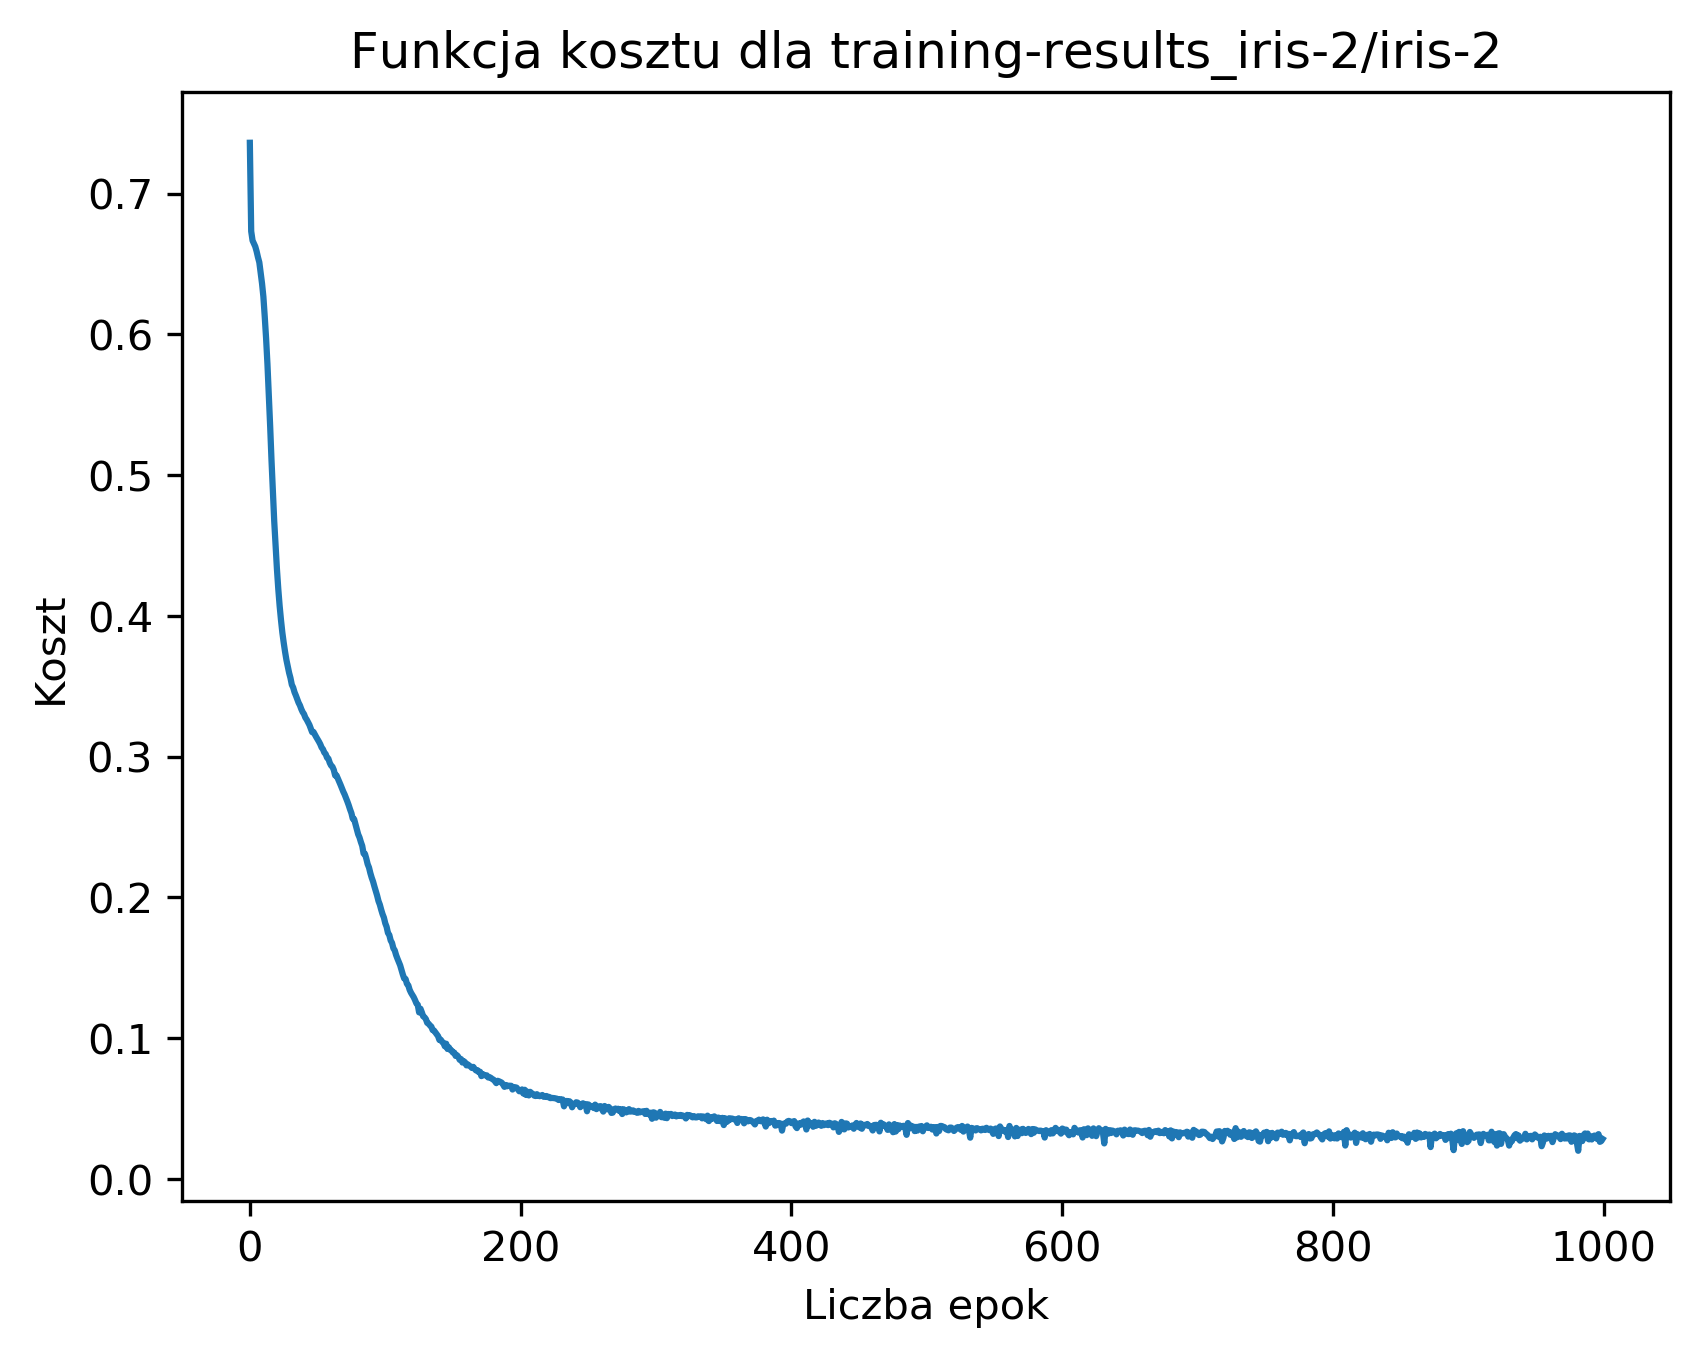
\includegraphics[width=110mm]{wykresy/iris-2_cost.png}
                    \caption{Tryb z normalizowanymi danymi}
                \end{figure}
                \begin{figure}[!htbp]
                    \centering
                    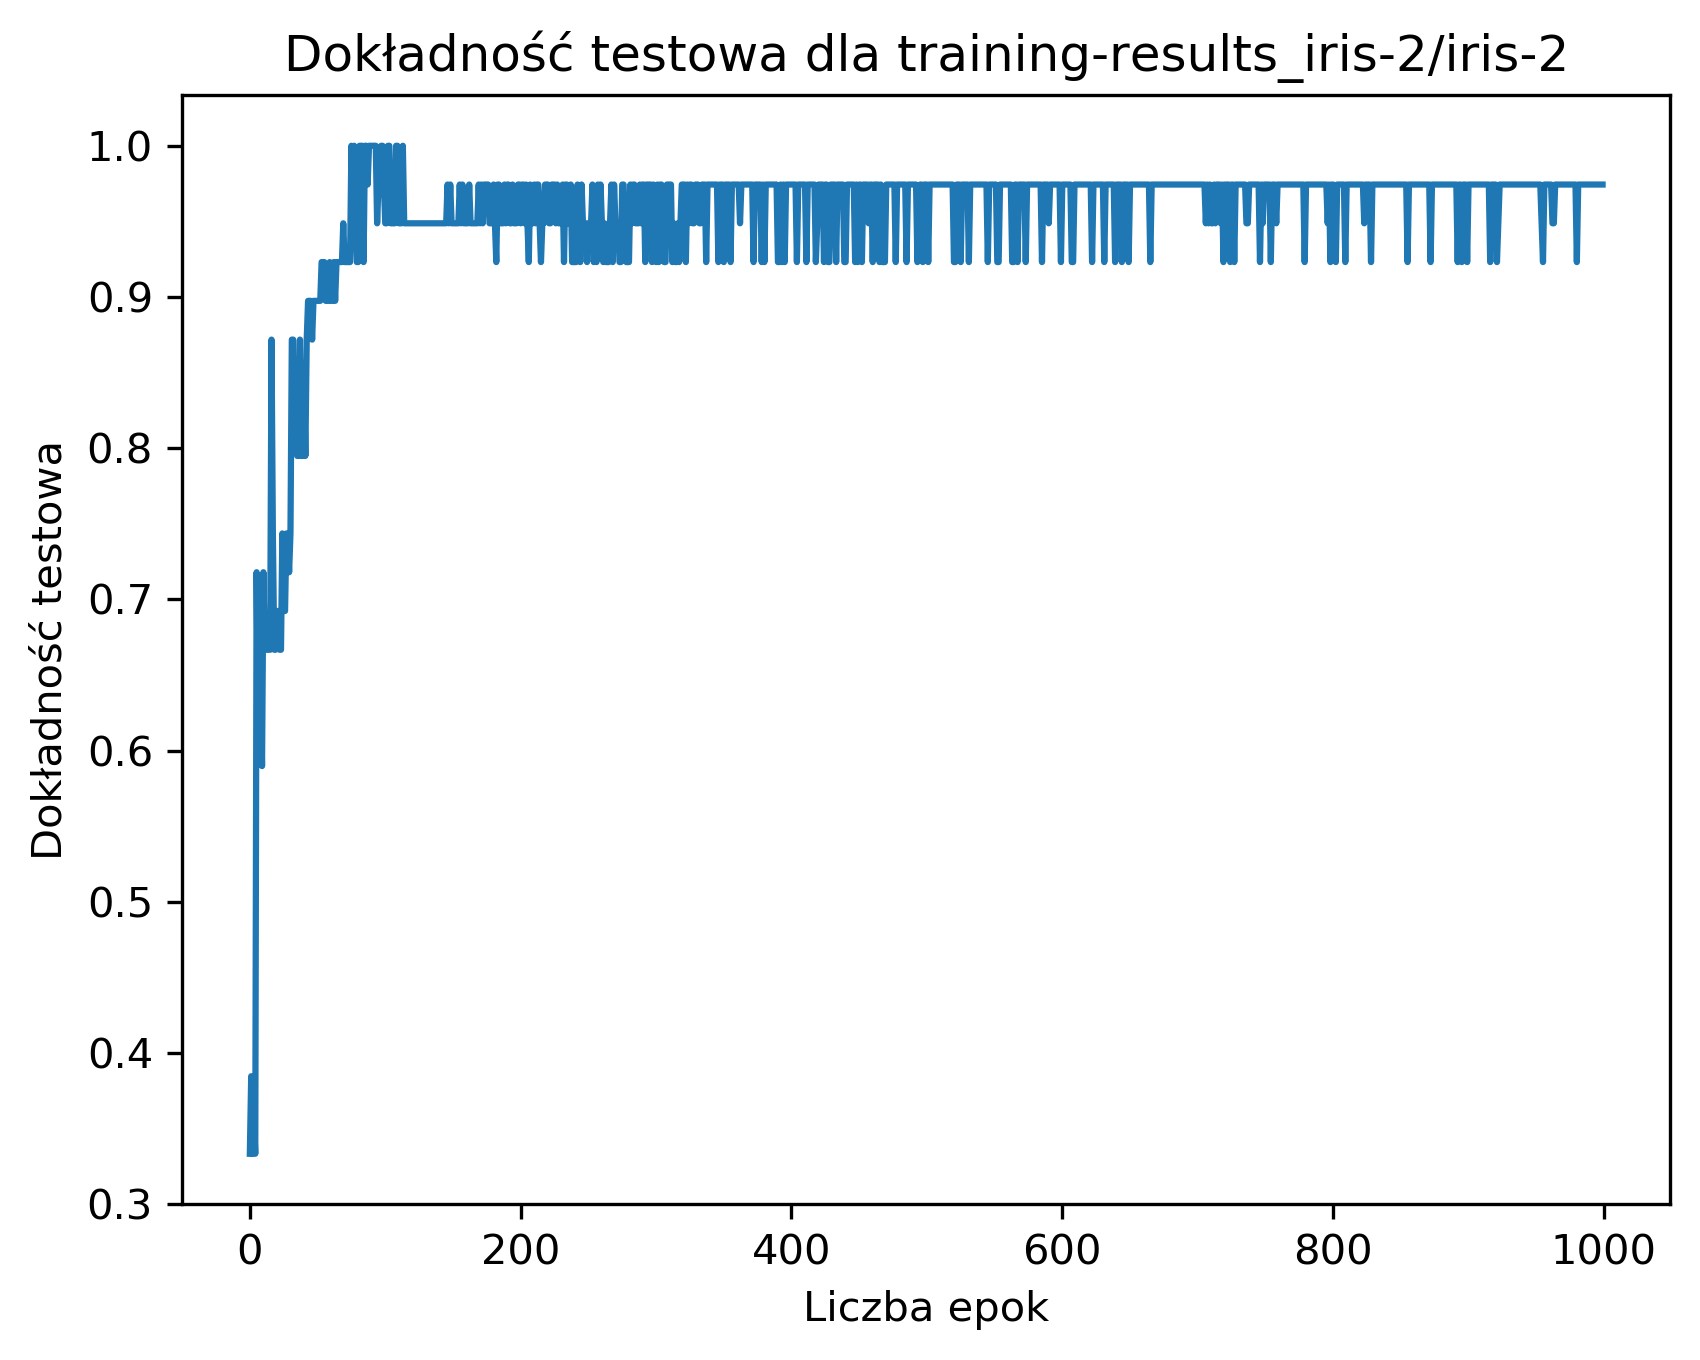
\includegraphics[width=110mm]{wykresy/iris-2_testing-accuracy.png}
                    \caption{Tryb z normalizowanymi danymi}
                \end{figure}
                \begin{figure}[!htbp]
                    \centering
                    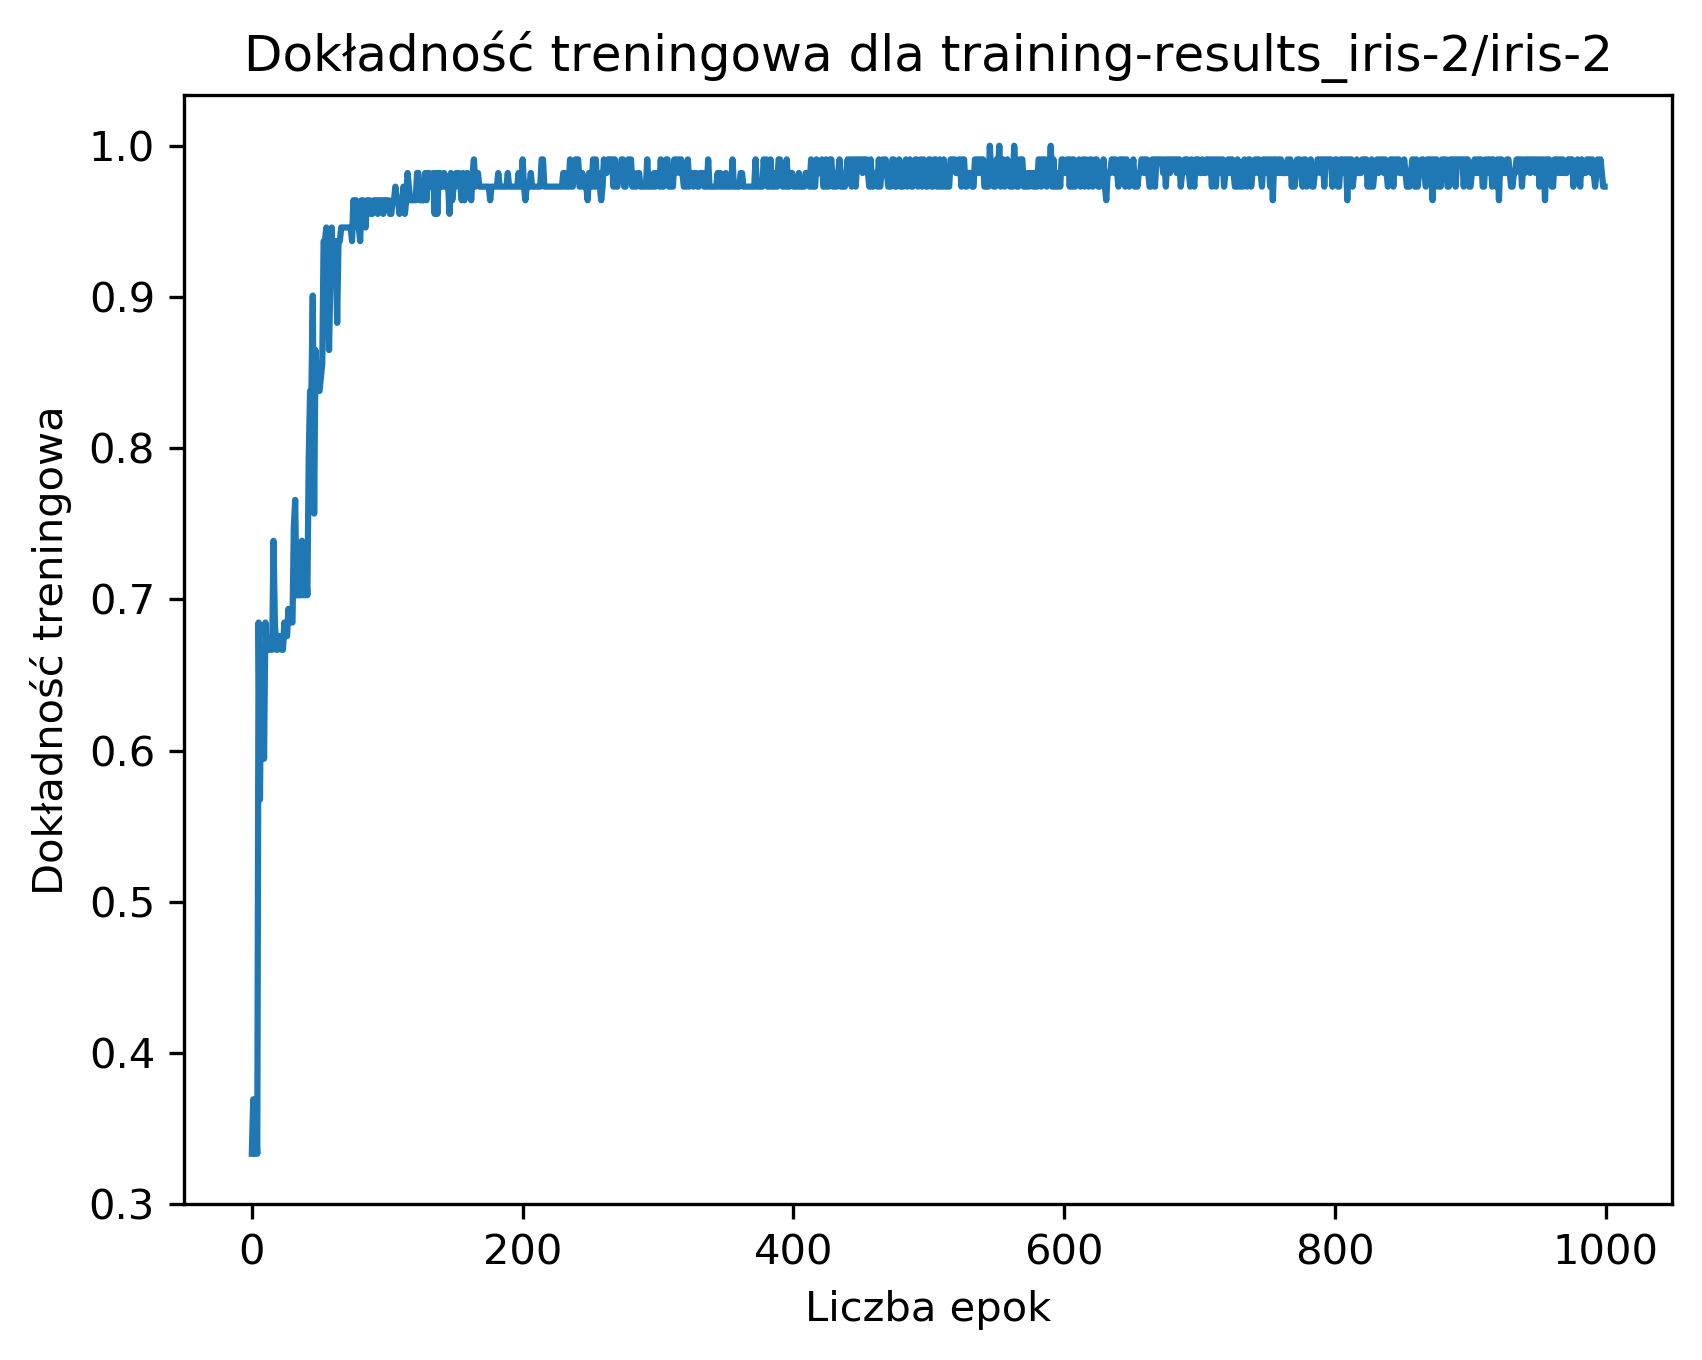
\includegraphics[width=110mm]{wykresy/iris-2_training-accuracy.png}
                    \caption{Tryb z normalizowanymi danymi}
                \end{figure}
                \FloatBarrier
            %---------------------------------------------------%
                \begin{figure}[!htbp]
                    \centering
                    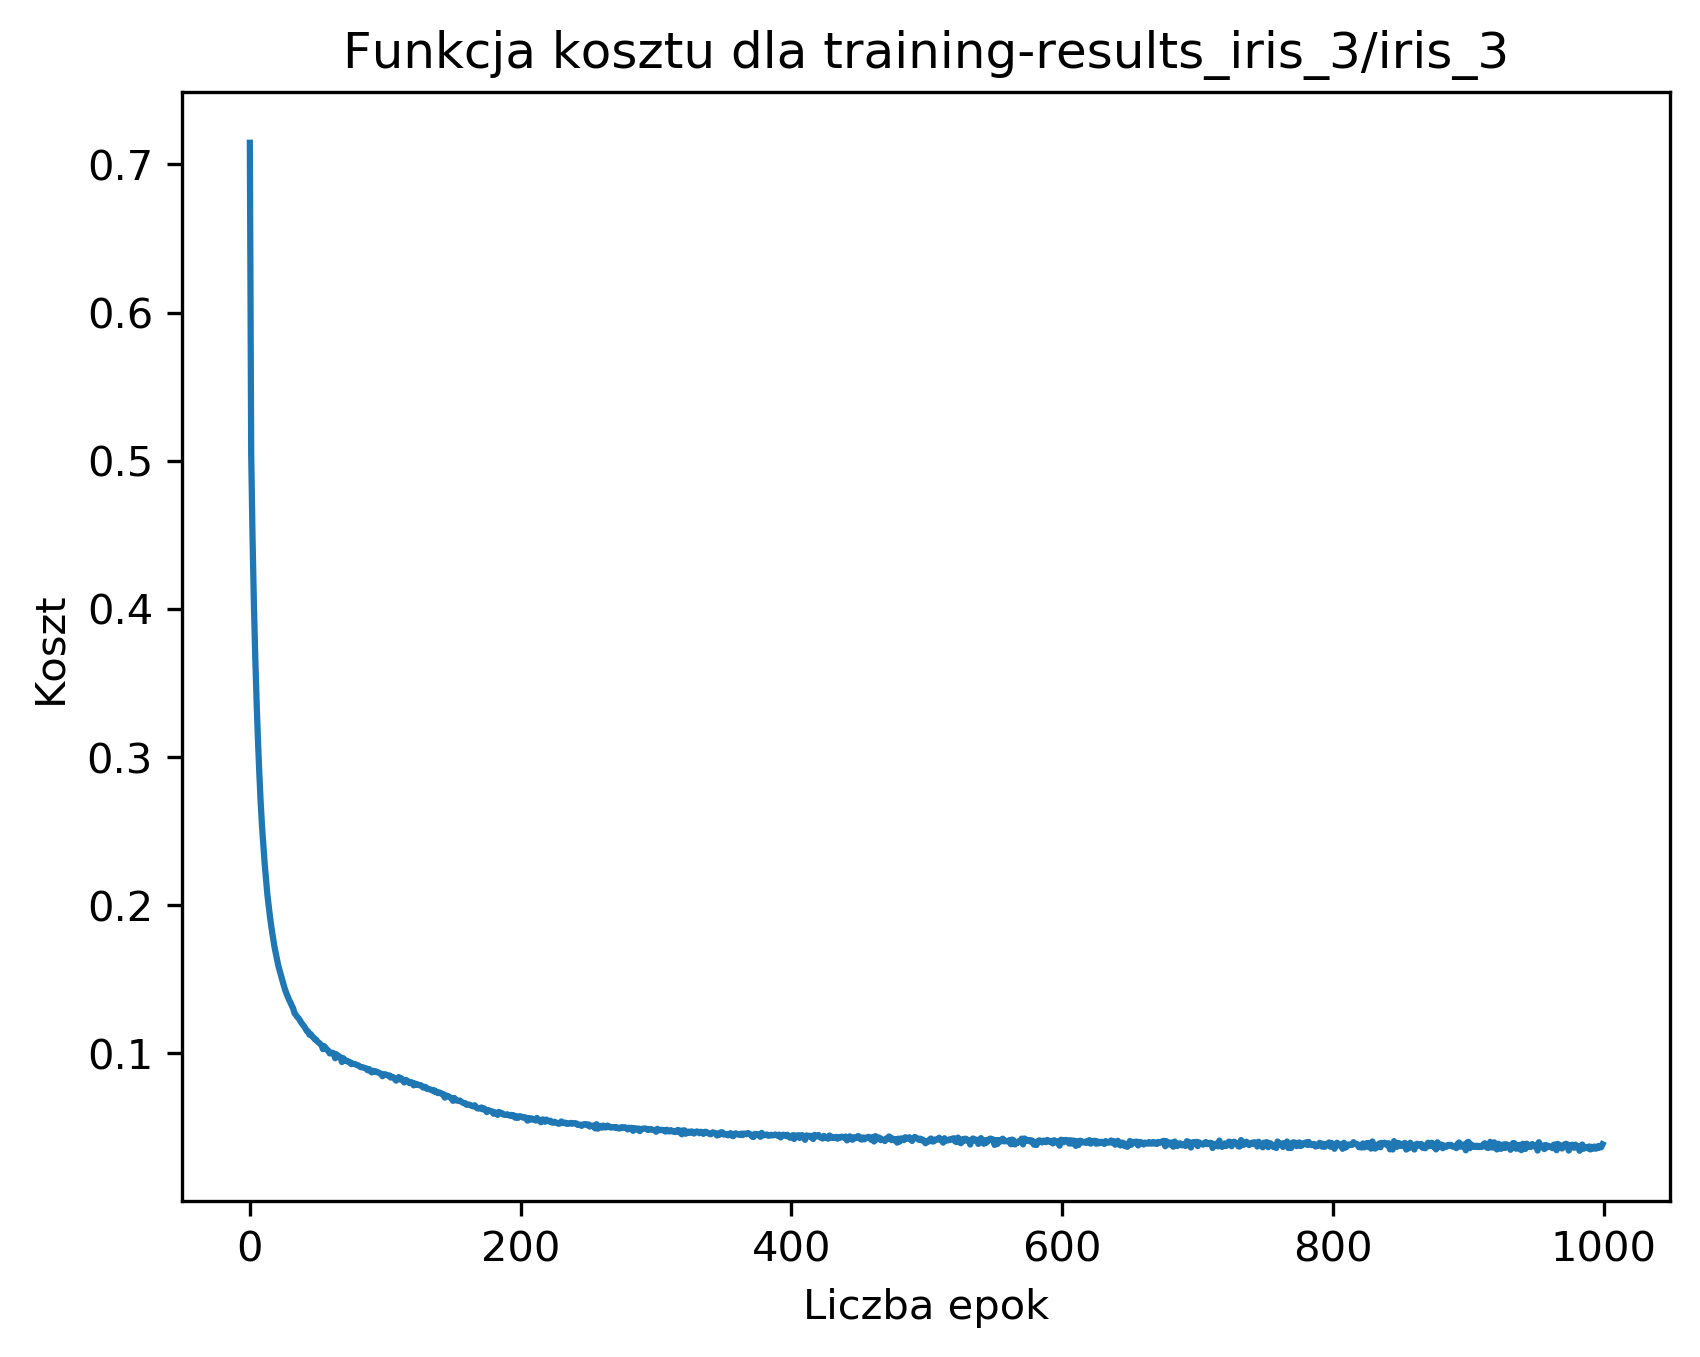
\includegraphics[width=110mm]{wykresy/iris_3_cost.png}
                    \caption{Tryb z standaryzowanymi danymi}
                \end{figure}
                \begin{figure}[!htbp]
                    \centering
                    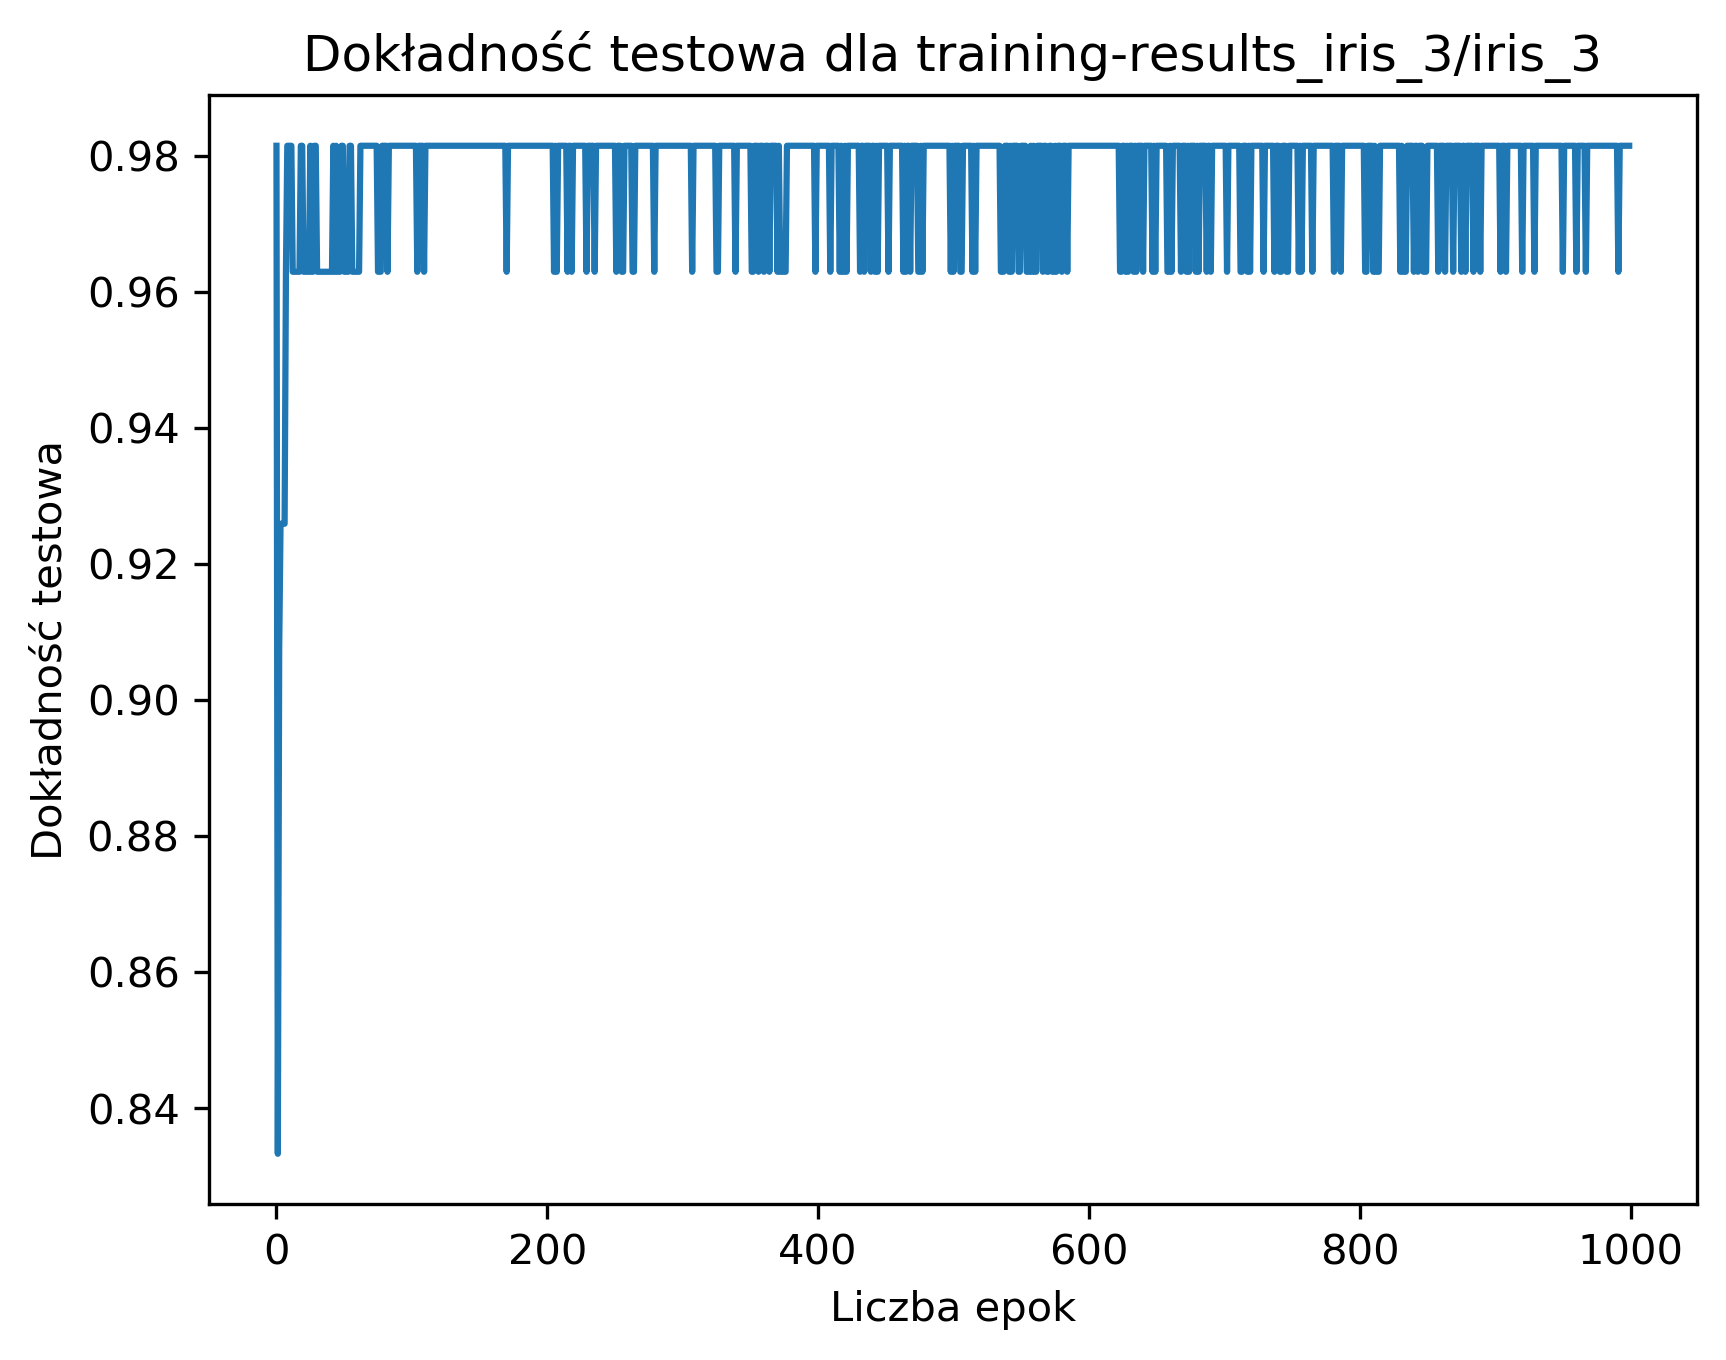
\includegraphics[width=110mm]{wykresy/iris_3_testing-accuracy.png}
                    \caption{Tryb z standaryzowanymi danymi}
                \end{figure}
                \begin{figure}[!htbp]
                    \centering
                    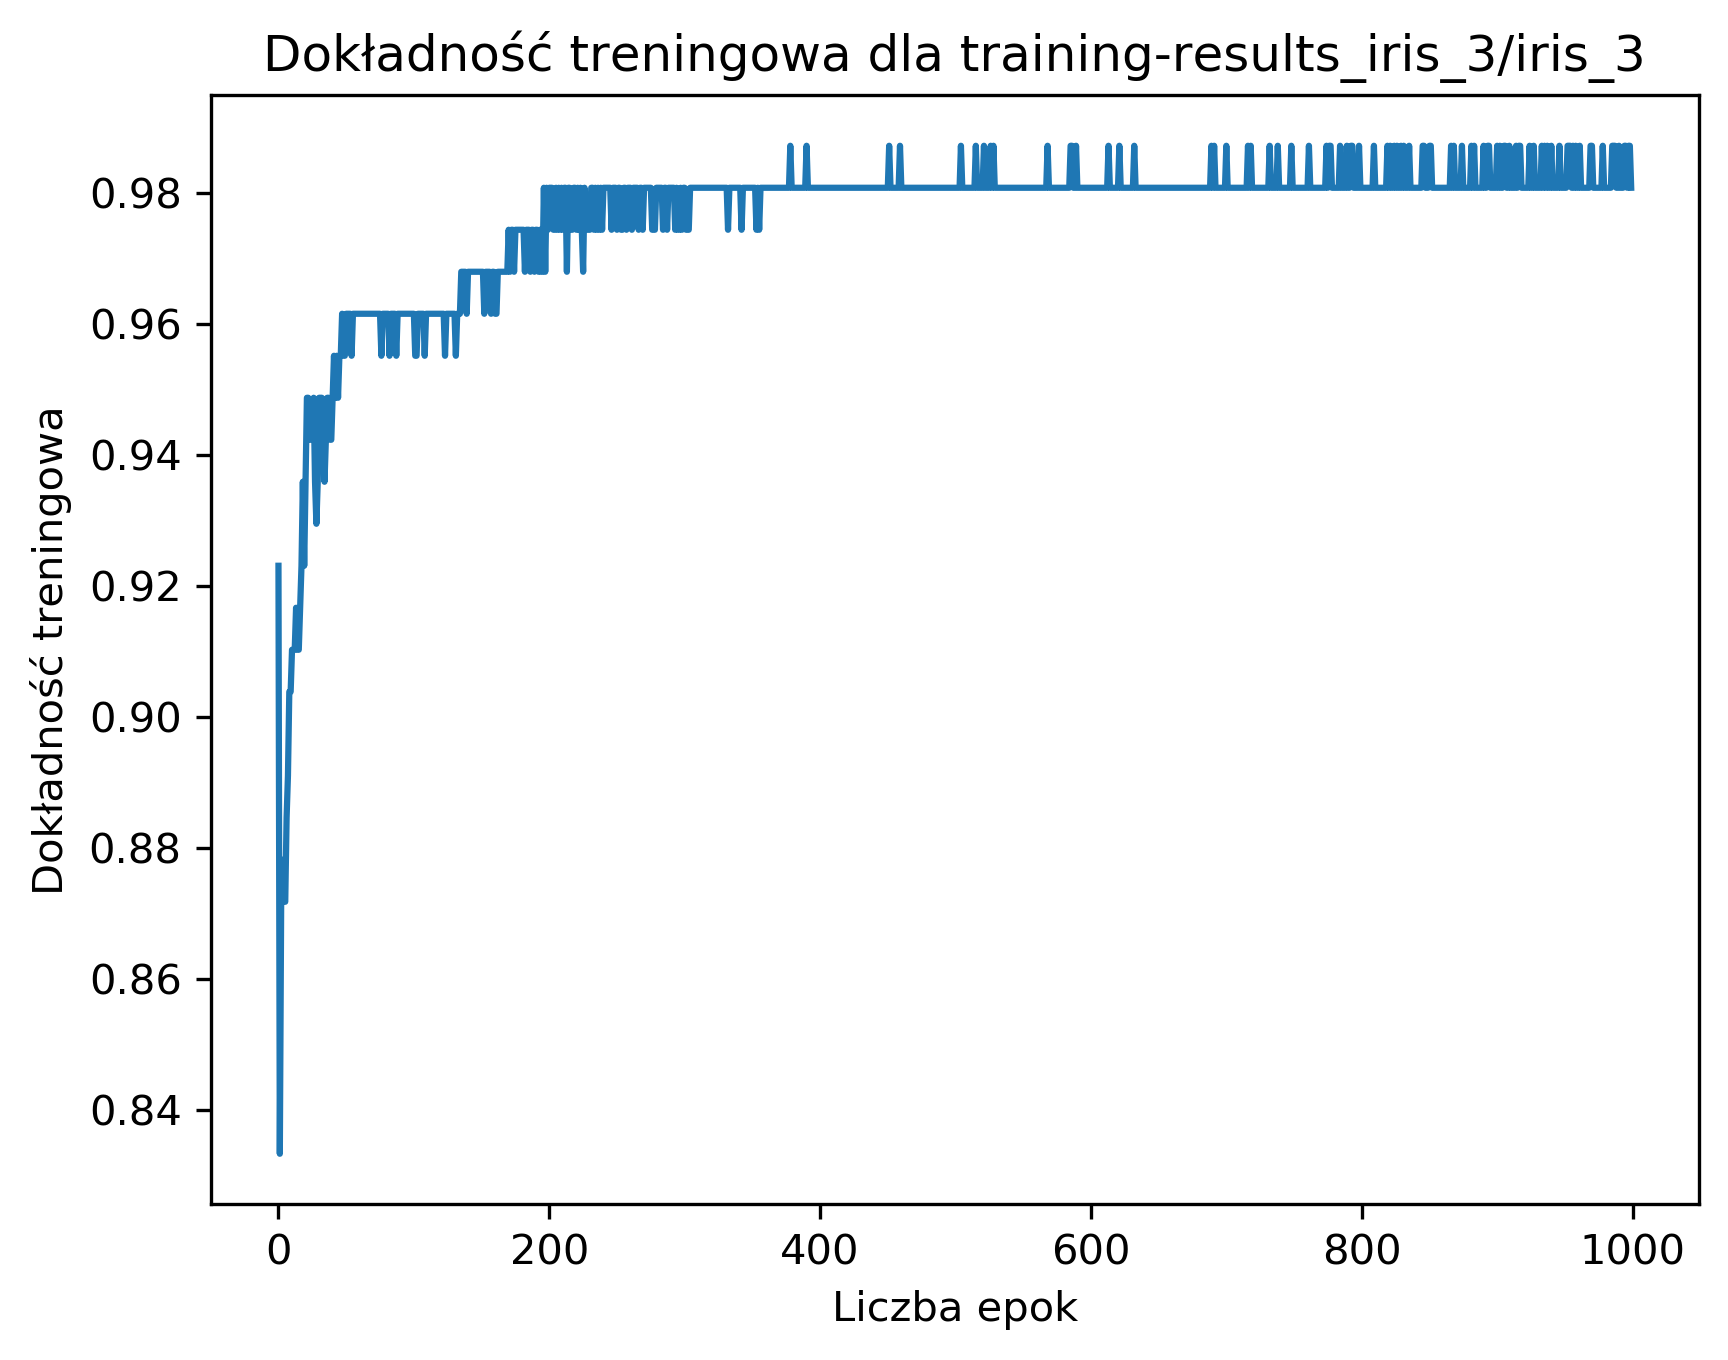
\includegraphics[width=110mm]{wykresy/iris_3_training-accuracy.png}
                    \caption{Tryb z standaryzowanymi danymi}
                \end{figure}
                \FloatBarrier
            %---------------------------------------------------%
            }
        %---------------------------------------------------%
            \subsubsection{K najbliższych sąsiadów - Zbiór testowy}
            {
                \textbf{Tryb danych domyślny, wartość K = 3}
                \begin{lstlisting}
>> ./data/iris-test.csv

> Global confusion matrix:
                [Iris-setosa][Iris-versicolor][Iris-virginica]
                [Iris-setosa]      20 0 0
                [Iris-versicolor]       0 19 1
                [Iris-virginica]       0 1 19


                Total population | 60

                Accuracy | 96.6667 %



                > [Iris-setosa]
                [Positive]    [Negative]
                [Positive]           20 0
                [Negative]            0 40


                Total population | 60

                True positive | 20
                True negative | 40
                False positive (type I error) | 0
                False negative (type II error) | 0

                Correct positive predictions | 100 %
                Correct negative predictions | 100 %

                Correct positive classifications | 100 %
                Correct negative classifications | 100 %

                Accuracy | 100 %



                > [Iris-versicolor]
                [Positive]    [Negative]
                [Positive]           19 1
                [Negative]            1 39


                Total population | 60

                True positive | 19
                True negative | 39
                False positive (type I error) | 1
                False negative (type II error) | 1

                Correct positive predictions | 95 %
                Correct negative predictions | 97.5 %

                Correct positive classifications | 95 %
                Correct negative classifications | 97.5 %

                Accuracy | 96.6667 %



                > [Iris-virginica]
                [Positive]    [Negative]
                [Positive]           19 1
                [Negative]            1 39


                Total population | 60

                True positive | 19
                True negative | 39
                False positive (type I error) | 1
                False negative (type II error) | 1

                Correct positive predictions | 95 %
                Correct negative predictions | 97.5 %

                Correct positive classifications | 95 %
                Correct negative classifications | 97.5 %

                Accuracy | 96.6667 %
                \end{lstlisting}
            %---------------------------------------------------%
                \textbf{Tryb danych domyślny, wartość K = 10}
                \begin{lstlisting}
>> ./data/iris-test.csv

> Global confusion matrix:
                [Iris-setosa][Iris-versicolor][Iris-virginica]
                [Iris-setosa]      20 0 0
                [Iris-versicolor]       0 20 3
                [Iris-virginica]       0 0 17


                Total population | 60

                Accuracy | 95 %



                > [Iris-setosa]
                [Positive]    [Negative]
                [Positive]           20 0
                [Negative]            0 40


                Total population | 60

                True positive | 20
                True negative | 40
                False positive (type I error) | 0
                False negative (type II error) | 0

                Correct positive predictions | 100 %
                Correct negative predictions | 100 %

                Correct positive classifications | 100 %
                Correct negative classifications | 100 %

                Accuracy | 100 %



                > [Iris-versicolor]
                [Positive]    [Negative]
                [Positive]           20 3
                [Negative]            0 37


                Total population | 60

                True positive | 20
                True negative | 37
                False positive (type I error) | 3
                False negative (type II error) | 0

                Correct positive predictions | 86.9565 %
                Correct negative predictions | 100 %

                Correct positive classifications | 100 %
                Correct negative classifications | 92.5 %

                Accuracy | 95 %



                > [Iris-virginica]
                [Positive]    [Negative]
                [Positive]           17 0
                [Negative]            3 40


                Total population | 60

                True positive | 17
                True negative | 40
                False positive (type I error) | 0
                False negative (type II error) | 3

                Correct positive predictions | 100 %
                Correct negative predictions | 93.0233 %

                Correct positive classifications | 85 %
                Correct negative classifications | 100 %

                Accuracy | 95 %

                \end{lstlisting}
            %---------------------------------------------------%
                \textbf{Tryb z normalizowanymi danymi, wartość K = 3}
                \begin{lstlisting}
>> ./data/iris-normalised-test.csv

> Global confusion matrix:
                [Iris-setosa][Iris-versicolor][Iris-virginica]
                [Iris-setosa]       20 0 0
                [Iris-versicolor]        0 19 2
                [Iris-virginica]        0 1 18


                Total population | 60

                Accuracy | 95 %



                > [Iris-setosa]
                [Positive]    [Negative]
                [Positive]           20 0
                [Negative]            0 40


                Total population | 60

                True positive | 20
                True negative | 40
                False positive (type I error) | 0
                False negative (type II error) | 0

                Correct positive predictions | 100 %
                Correct negative predictions | 100 %

                Correct positive classifications | 100 %
                Correct negative classifications | 100 %

                Accuracy | 100 %



                > [Iris-versicolor]
                [Positive]    [Negative]
                [Positive]           19 2
                [Negative]            1 38


                Total population | 60

                True positive | 19
                True negative | 38
                False positive (type I error) | 2
                False negative (type II error) | 1

                Correct positive predictions | 90.4762 %
                Correct negative predictions | 97.4359 %

                Correct positive classifications | 95 %
                Correct negative classifications | 95 %

                Accuracy | 95 %



                > [Iris-virginica]
                [Positive]    [Negative]
                [Positive]           18 1
                [Negative]            2 39


                Total population | 60

                True positive | 18
                True negative | 39
                False positive (type I error) | 1
                False negative (type II error) | 2

                Correct positive predictions | 94.7368 %
                Correct negative predictions | 95.122 %

                Correct positive classifications | 90 %
                Correct negative classifications | 97.5 %

                Accuracy | 95 %

                \end{lstlisting}
            %---------------------------------------------------%
                \textbf{Tryb z normalizowanymi danymi, wartość K = 5}
                \begin{lstlisting}
>> ./data/iris-normalised-test.csv

> Global confusion matrix:
                [Iris-setosa][Iris-versicolor][Iris-virginica]
                [Iris-setosa]       20 0 0
                [Iris-versicolor]        0 20 1
                [Iris-virginica]        0 0 19


                Total population | 60

                Accuracy | 98.3333 %



                > [Iris-setosa]
                [Positive]    [Negative]
                [Positive]           20 0
                [Negative]            0 40


                Total population | 60

                True positive | 20
                True negative | 40
                False positive (type I error) | 0
                False negative (type II error) | 0

                Correct positive predictions | 100 %
                Correct negative predictions | 100 %

                Correct positive classifications | 100 %
                Correct negative classifications | 100 %

                Accuracy | 100 %



                > [Iris-versicolor]
                [Positive]    [Negative]
                [Positive]           20 1
                [Negative]            0 39


                Total population | 60

                True positive | 20
                True negative | 39
                False positive (type I error) | 1
                False negative (type II error) | 0

                Correct positive predictions | 95.2381 %
                Correct negative predictions | 100 %

                Correct positive classifications | 100 %
                Correct negative classifications | 97.5 %

                Accuracy | 98.3333 %



                > [Iris-virginica]
                [Positive]    [Negative]
                [Positive]           19 0
                [Negative]            1 40


                Total population | 60

                True positive | 19
                True negative | 40
                False positive (type I error) | 0
                False negative (type II error) | 1

                Correct positive predictions | 100 %
                Correct negative predictions | 97.561 %

                Correct positive classifications | 95 %
                Correct negative classifications | 100 %

                Accuracy | 98.3333 %

                \end{lstlisting}
            %---------------------------------------------------%
                \textbf{Tryb z standaryzowanymi danymi, wartość K = 1}
                \begin{lstlisting}
>> ./data/iris-standardised-test.csv

> Global confusion matrix:
                [Iris-setosa][Iris-versicolor][Iris-virginica]
                [Iris-setosa]      19 0 0
                [Iris-versicolor]       1 19 1
                [Iris-virginica]       0 1 19


                Total population | 60

                Accuracy | 95 %



                > [Iris-setosa]
                [Positive]    [Negative]
                [Positive]           19 0
                [Negative]            1 40


                Total population | 60

                True positive | 19
                True negative | 40
                False positive (type I error) | 0
                False negative (type II error) | 1

                Correct positive predictions | 100 %
                Correct negative predictions | 97.561 %

                Correct positive classifications | 95 %
                Correct negative classifications | 100 %

                Accuracy | 98.3333 %



                > [Iris-versicolor]
                [Positive]    [Negative]
                [Positive]           19 2
                [Negative]            1 38


                Total population | 60

                True positive | 19
                True negative | 38
                False positive (type I error) | 2
                False negative (type II error) | 1

                Correct positive predictions | 90.4762 %
                Correct negative predictions | 97.4359 %

                Correct positive classifications | 95 %
                Correct negative classifications | 95 %

                Accuracy | 95 %



                > [Iris-virginica]
                [Positive]    [Negative]
                [Positive]           19 1
                [Negative]            1 39


                Total population | 60

                True positive | 19
                True negative | 39
                False positive (type I error) | 1
                False negative (type II error) | 1

                Correct positive predictions | 95 %
                Correct negative predictions | 97.5 %

                Correct positive classifications | 95 %
                Correct negative classifications | 97.5 %

                Accuracy | 96.6667 %

                \end{lstlisting}
            %---------------------------------------------------%
                \textbf{Tryb z standaryzowanymi danymi, wartość K = 10}
                \begin{lstlisting}
>> ./data/iris-standardised-test.csv

> Global confusion matrix:
                [Iris-setosa][Iris-versicolor][Iris-virginica]
                [Iris-setosa]      20 0 0
                [Iris-versicolor]       0 19 3
                [Iris-virginica]       0 1 17


                Total population | 60

                Accuracy | 93.3333 %



                > [Iris-setosa]
                [Positive]    [Negative]
                [Positive]           20 0
                [Negative]            0 40


                Total population | 60

                True positive | 20
                True negative | 40
                False positive (type I error) | 0
                False negative (type II error) | 0

                Correct positive predictions | 100 %
                Correct negative predictions | 100 %

                Correct positive classifications | 100 %
                Correct negative classifications | 100 %

                Accuracy | 100 %



                > [Iris-versicolor]
                [Positive]    [Negative]
                [Positive]           19 3
                [Negative]            1 37


                Total population | 60

                True positive | 19
                True negative | 37
                False positive (type I error) | 3
                False negative (type II error) | 1

                Correct positive predictions | 86.3636 %
                Correct negative predictions | 97.3684 %

                Correct positive classifications | 95 %
                Correct negative classifications | 92.5 %

                Accuracy | 93.3333 %



                > [Iris-virginica]
                [Positive]    [Negative]
                [Positive]           17 1
                [Negative]            3 39


                Total population | 60

                True positive | 17
                True negative | 39
                False positive (type I error) | 1
                False negative (type II error) | 3

                Correct positive predictions | 94.4444 %
                Correct negative predictions | 92.8571 %

                Correct positive classifications | 85 %
                Correct negative classifications | 97.5 %

                Accuracy | 93.3333 %

                \end{lstlisting}
            %---------------------------------------------------%
            }
        }
    %---------------------------------------------------%
        \subsection{Zbior Nasion}
        {
            \subsubsection{Perceptron wielowarstwowy}
            {
                Poniżej znajdują się wykresy dla trzech trybów

                \begin{figure}[!htbp]
                    \centering
                    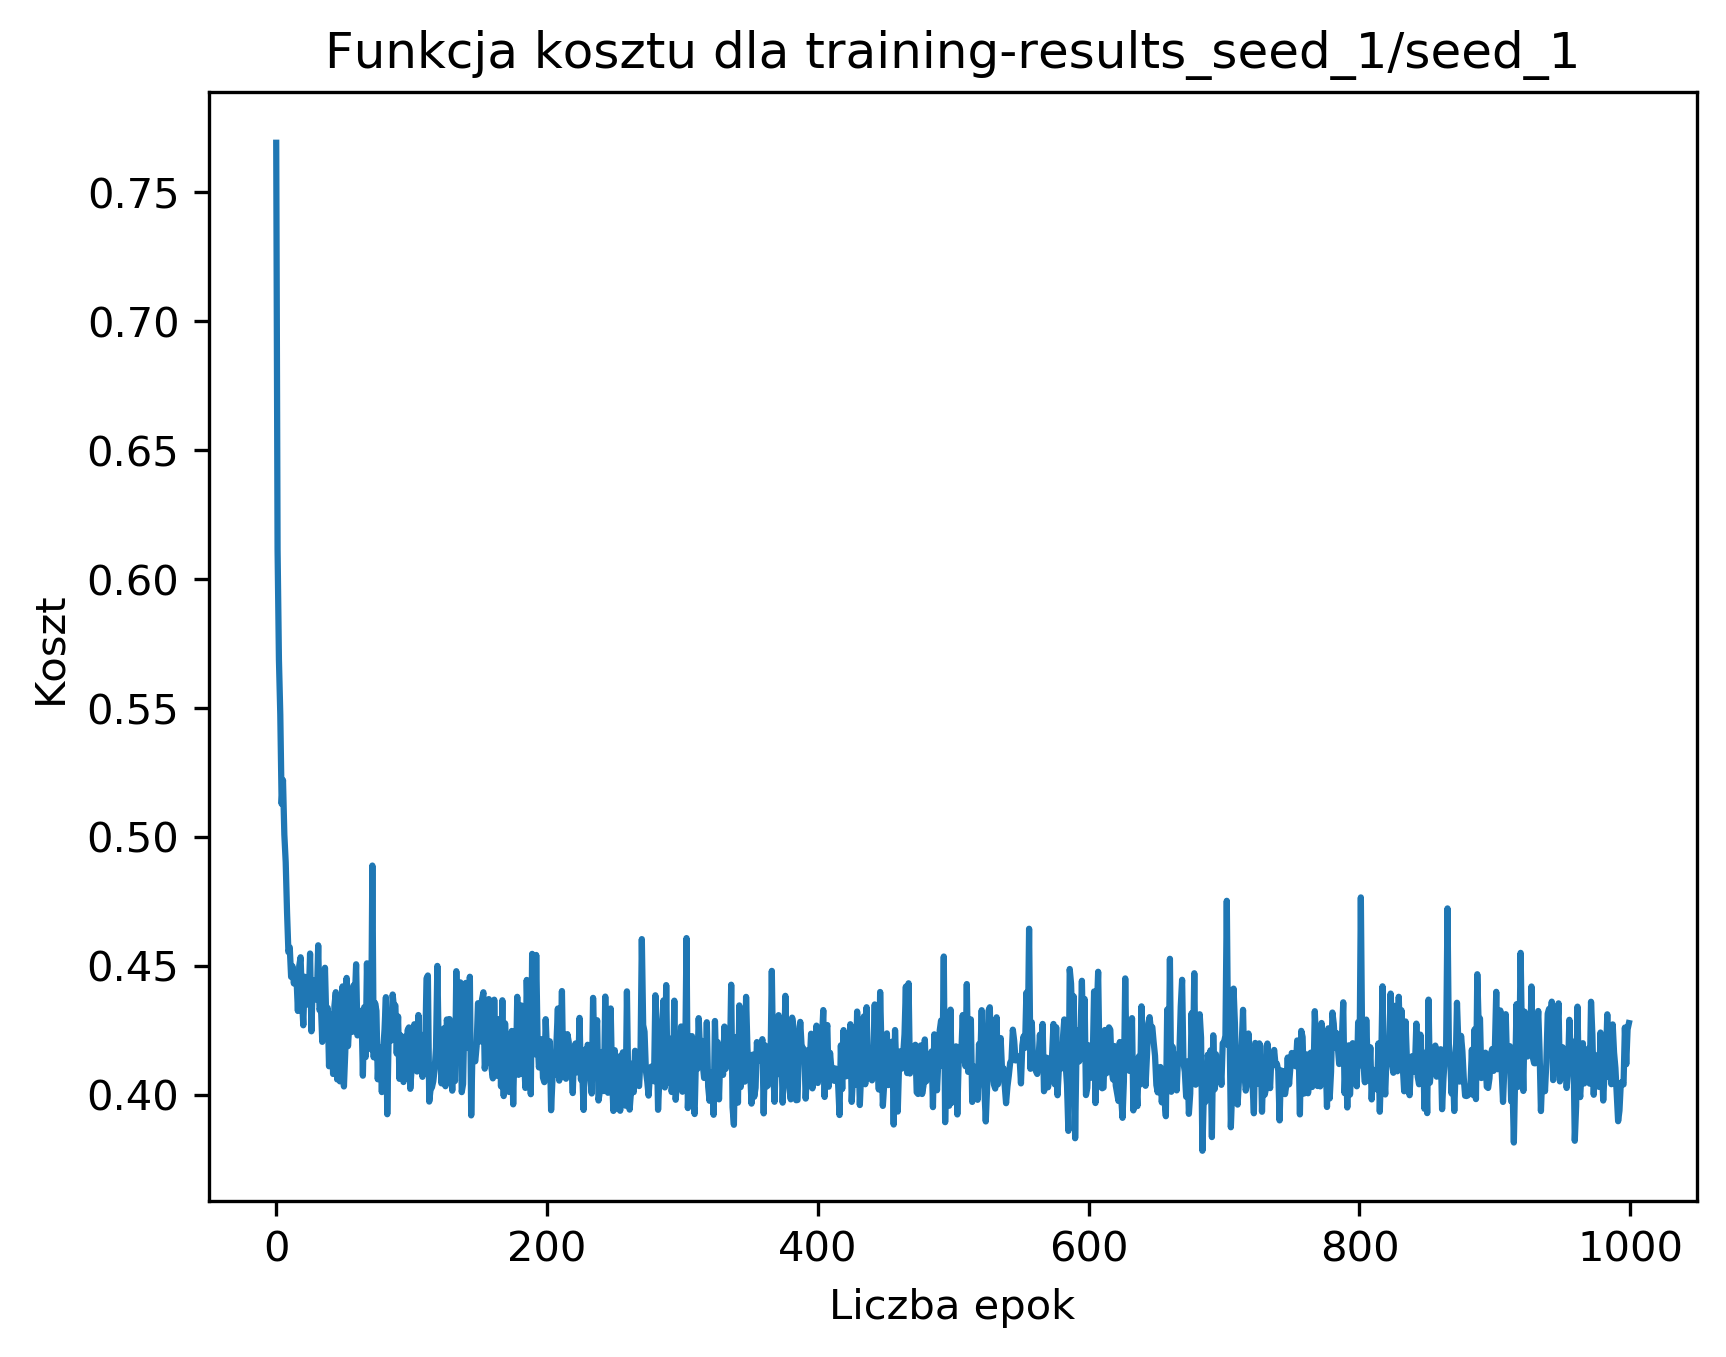
\includegraphics[width=110mm]{wykresy/seed_1_cost.png}
                    \caption{Tryb z domyślnymi danymi}
                \end{figure}
                \begin{figure}[!htbp]
                    \centering
                    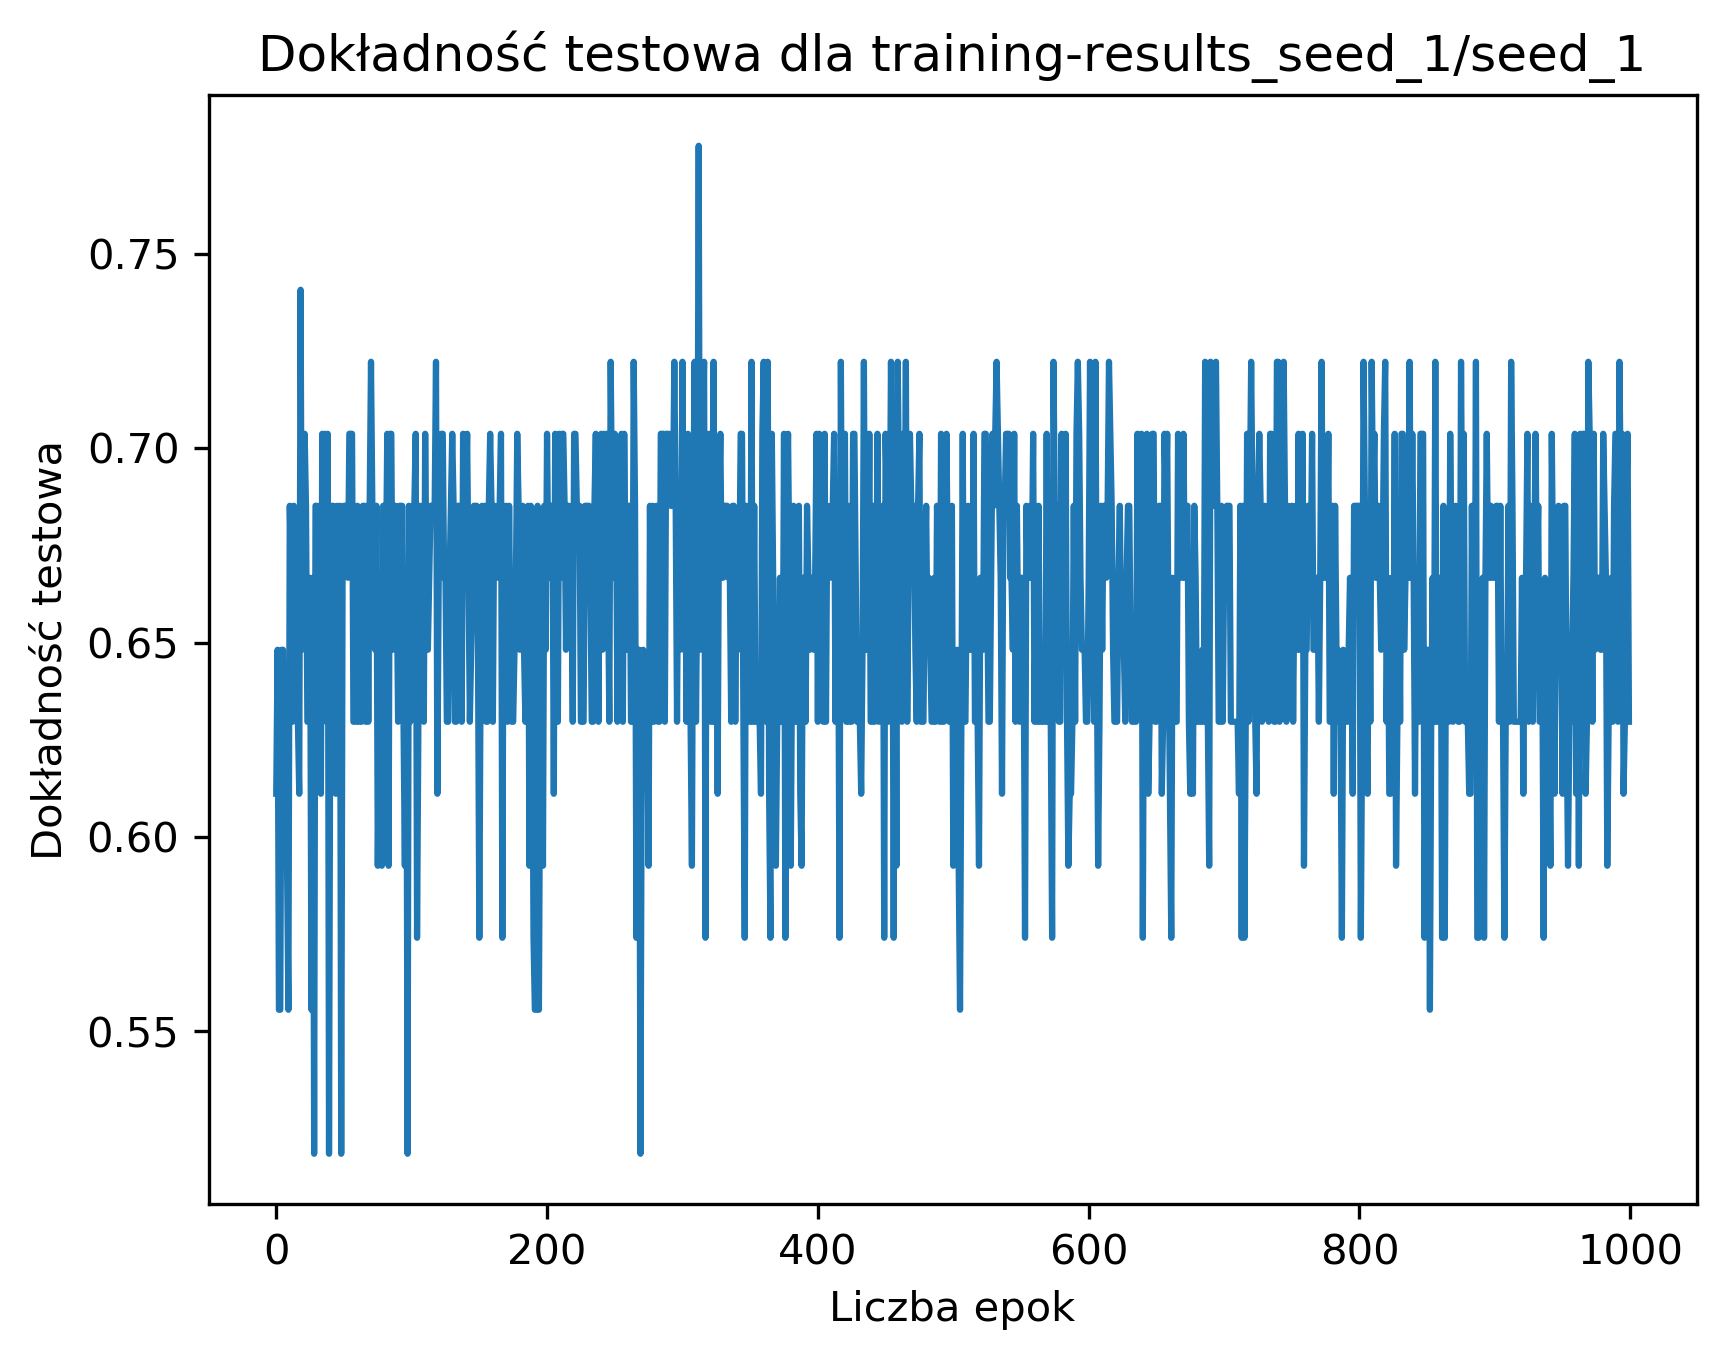
\includegraphics[width=110mm]{wykresy/seed_1_testing-accuracy.png}
                    \caption{Tryb z domyślnymi danymi}
                \end{figure}
                \begin{figure}[!htbp]
                    \centering
                    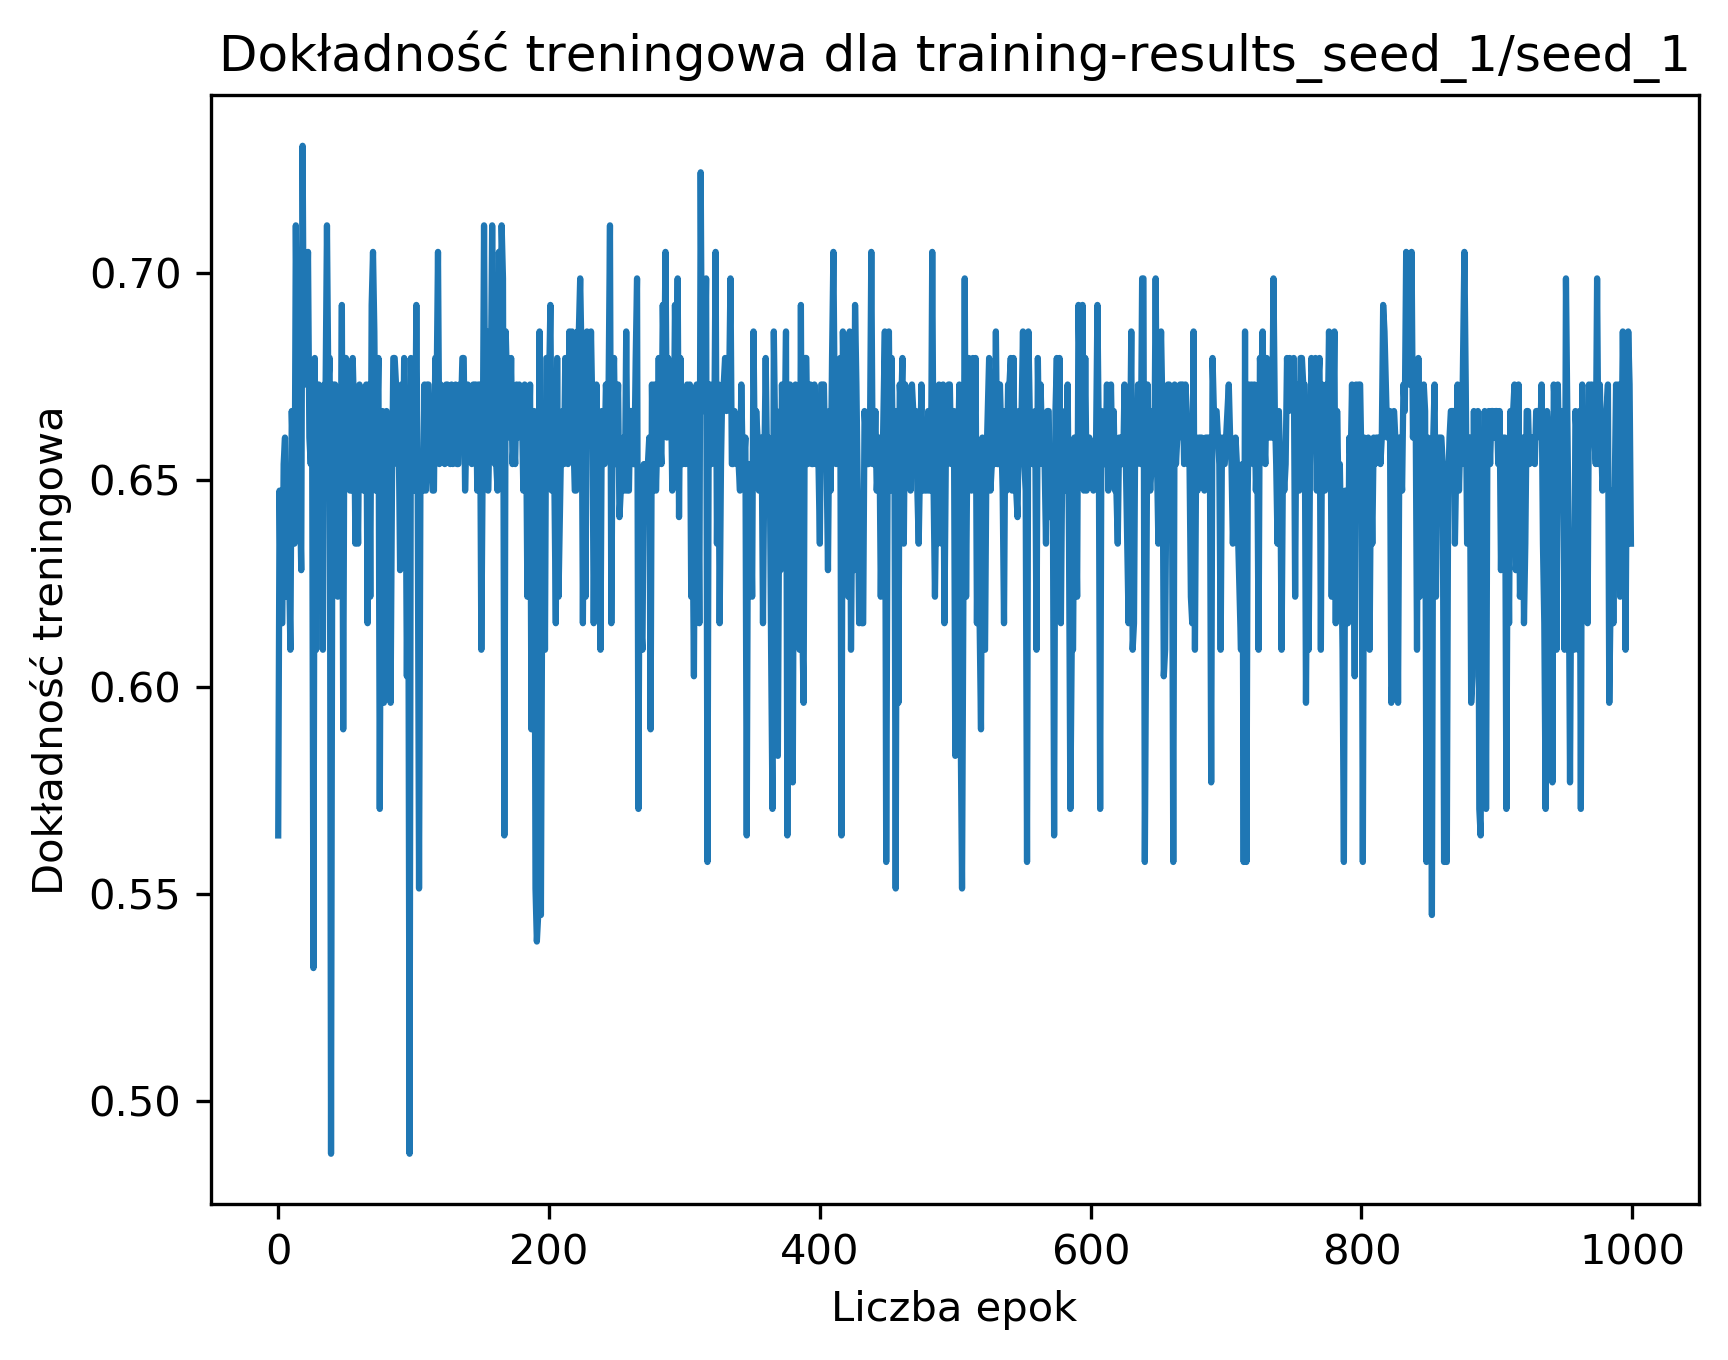
\includegraphics[width=110mm]{wykresy/seed_1_training-accuracy.png}
                    \caption{Tryb z domyślnymi danymi}
                \end{figure}
                \FloatBarrier
            %---------------------------------------------------%
                \begin{figure}[!htbp]
                    \centering
                    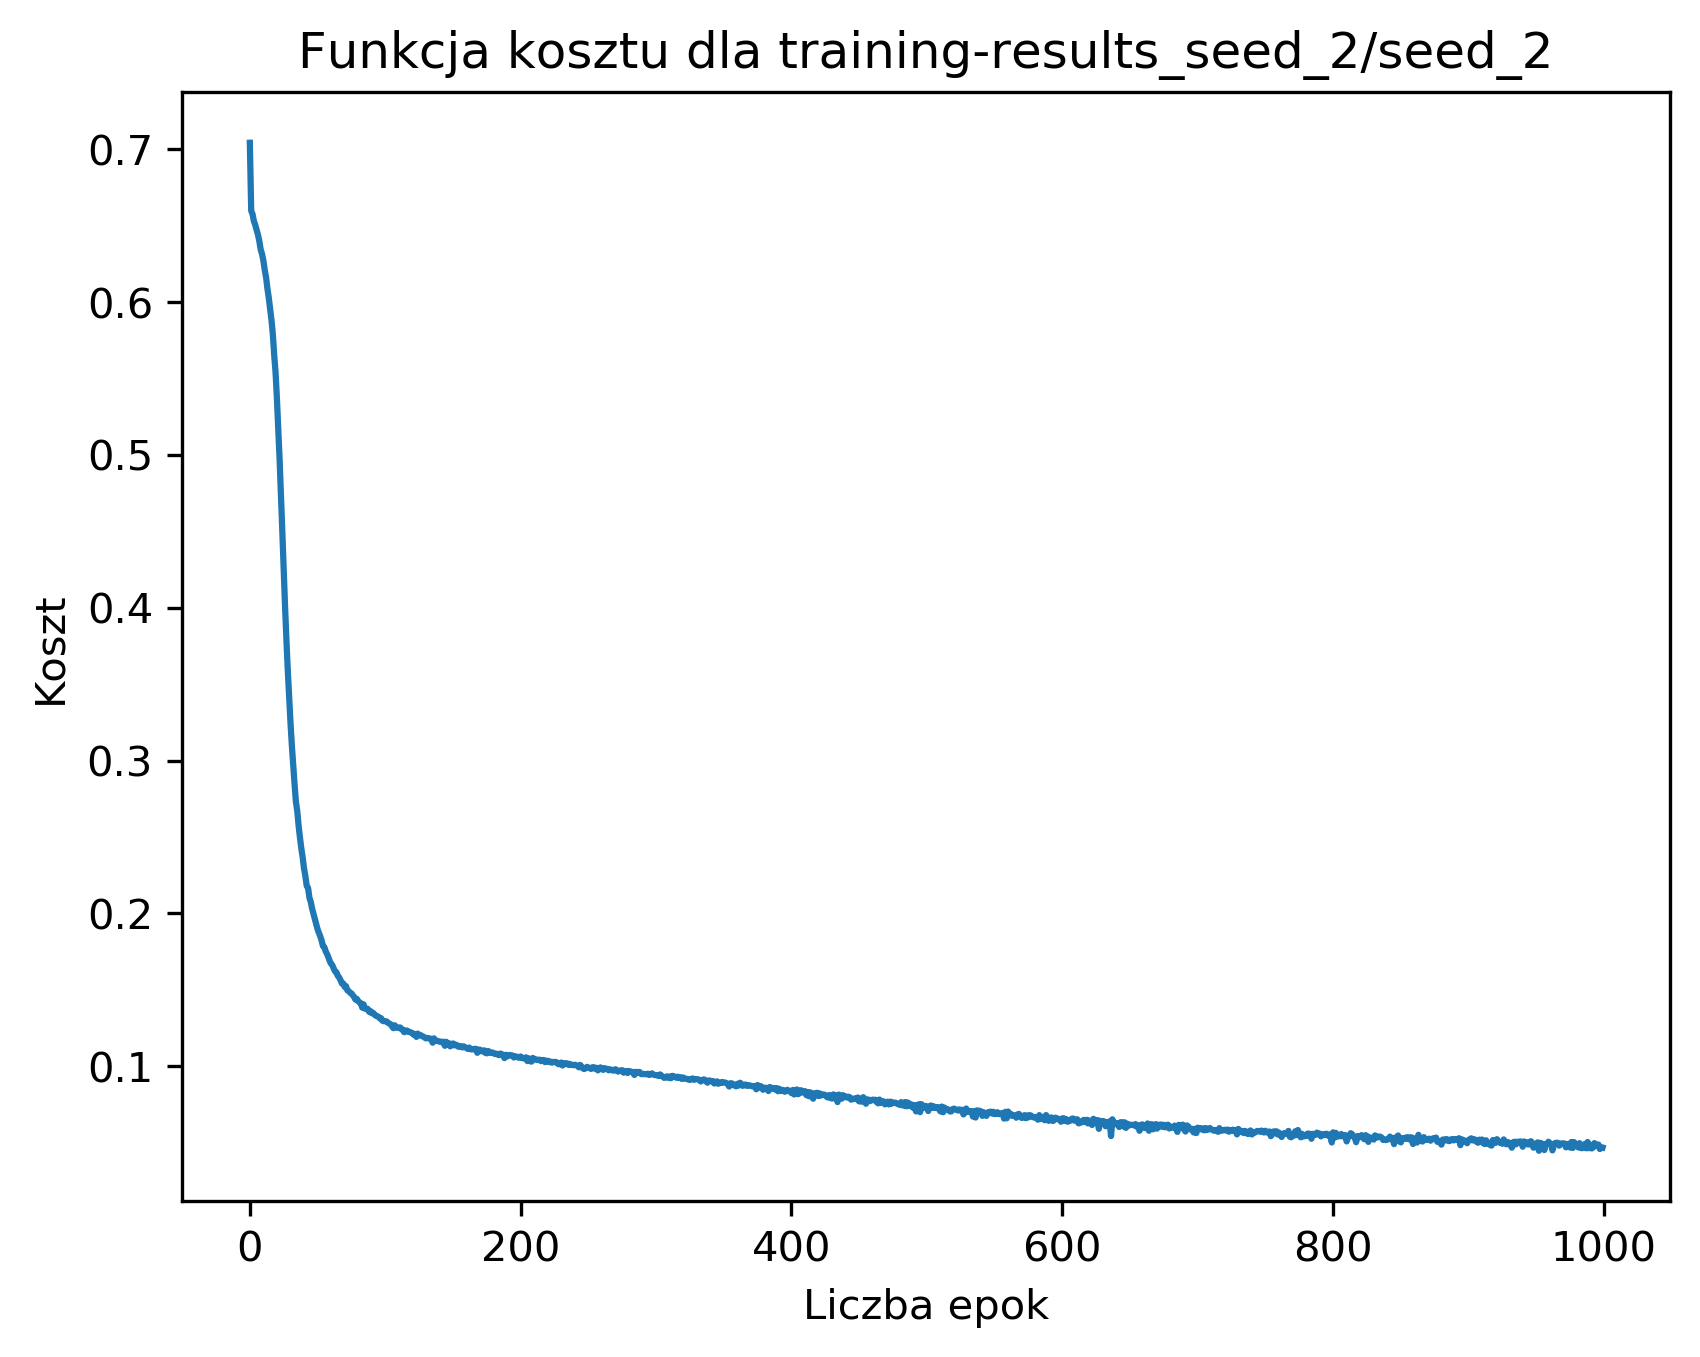
\includegraphics[width=110mm]{wykresy/seed_2_cost.png}
                    \caption{Tryb z normalizowanymi danymi}
                \end{figure}
                \begin{figure}[!htbp]
                    \centering
                    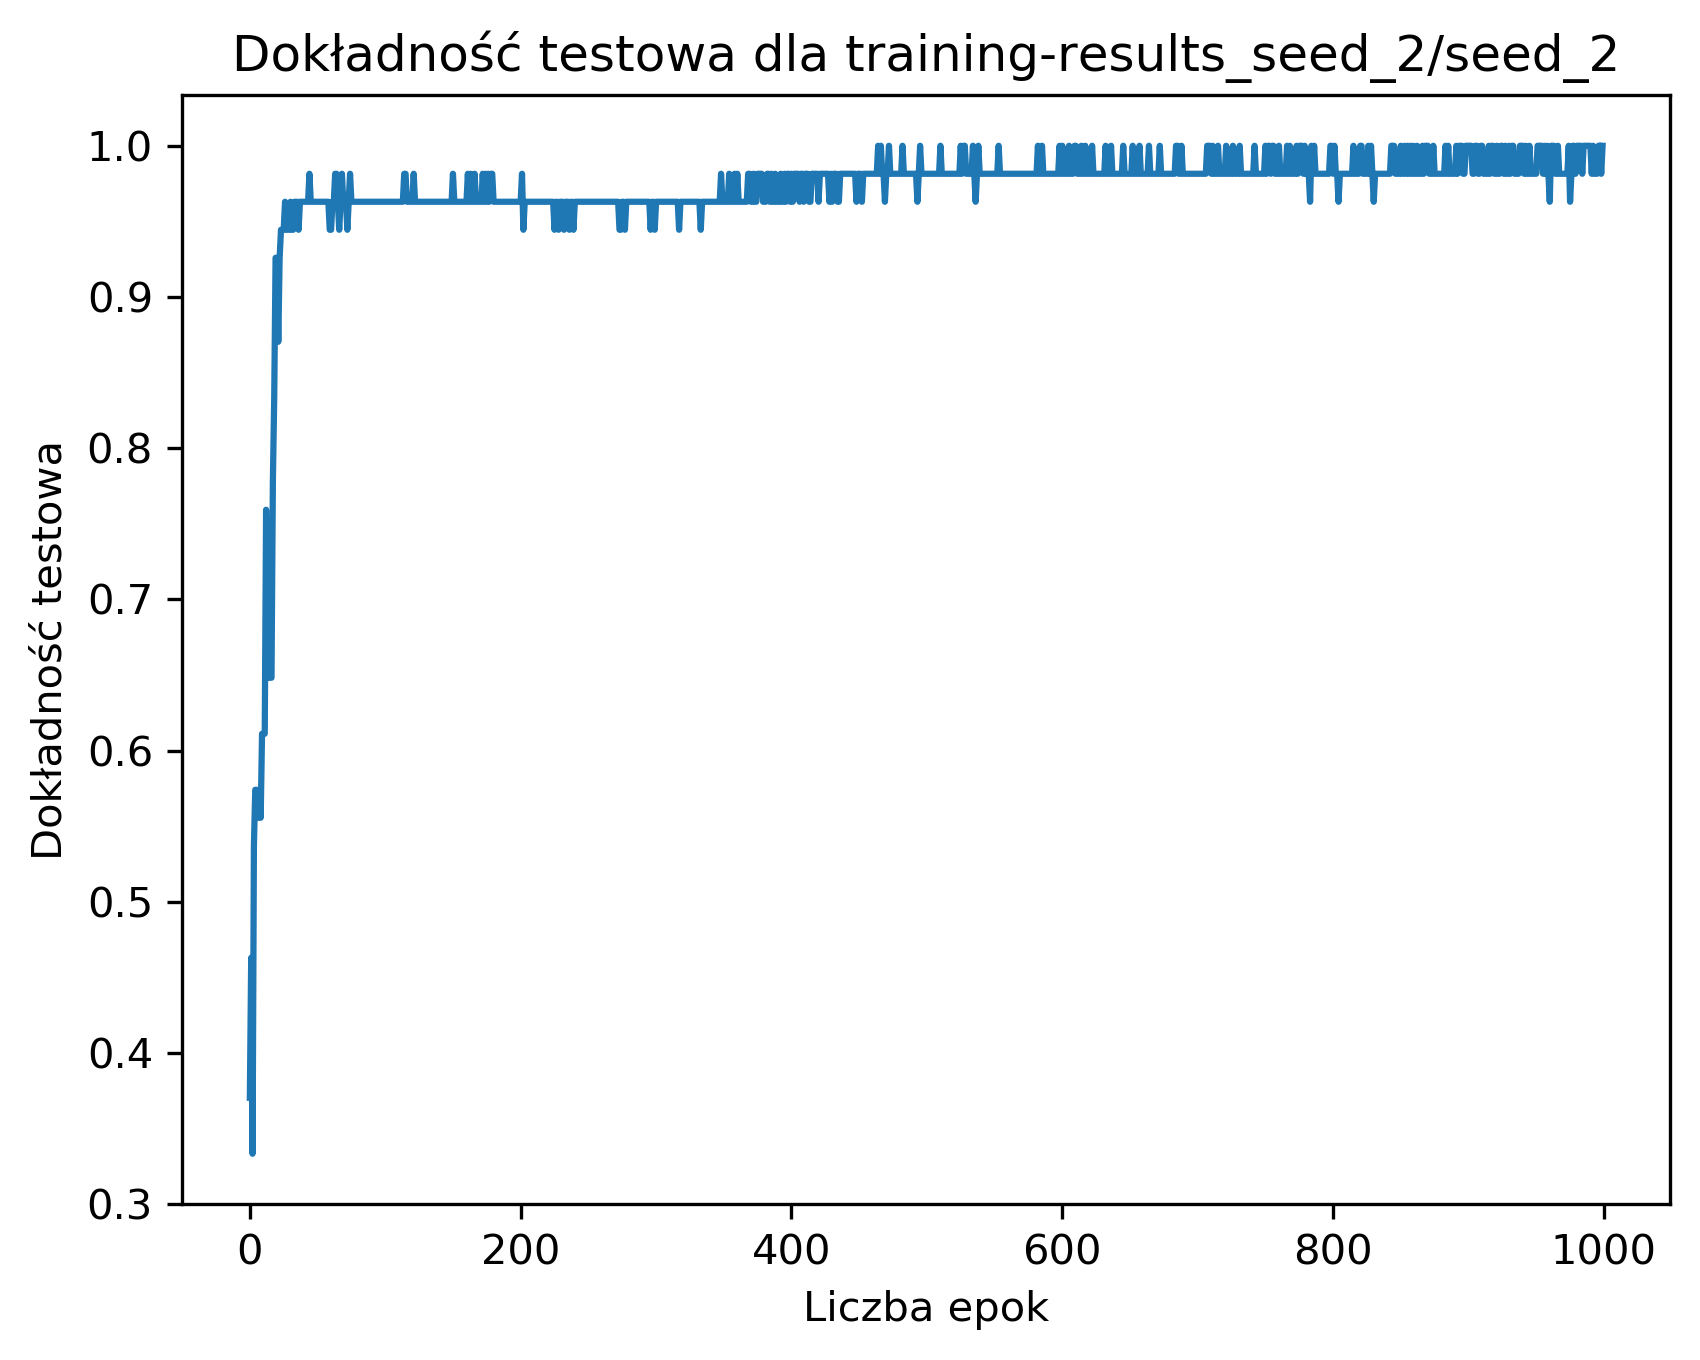
\includegraphics[width=110mm]{wykresy/seed_2_testing-accuracy.png}
                    \caption{Tryb z normalizowanymi danymi}
                \end{figure}
                \begin{figure}[!htbp]
                    \centering
                    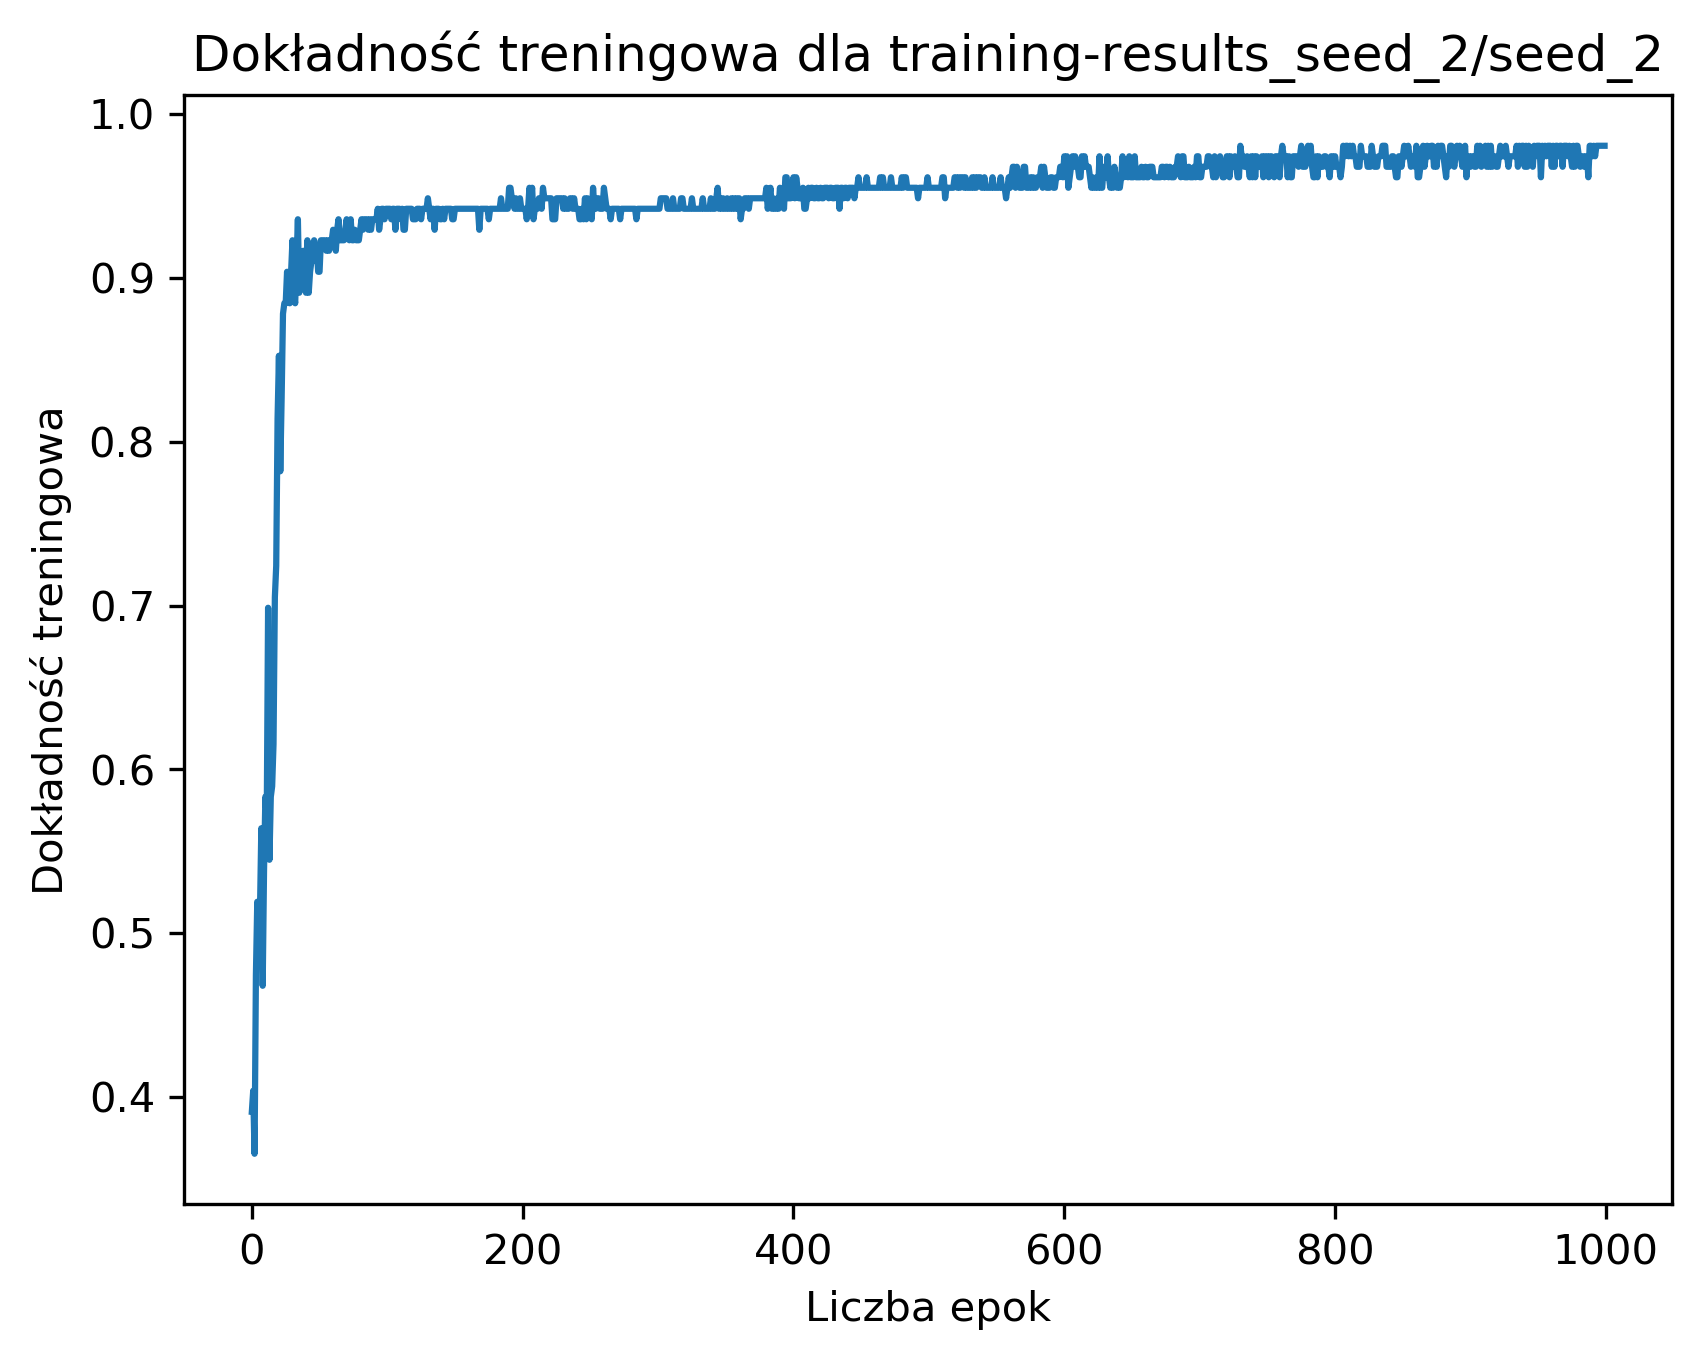
\includegraphics[width=110mm]{wykresy/seed_2_training-accuracy.png}
                    \caption{Tryb z normalizowanymi danymi}
                \end{figure}
                \FloatBarrier
            %---------------------------------------------------%
                \begin{figure}[!htbp]
                    \centering
                    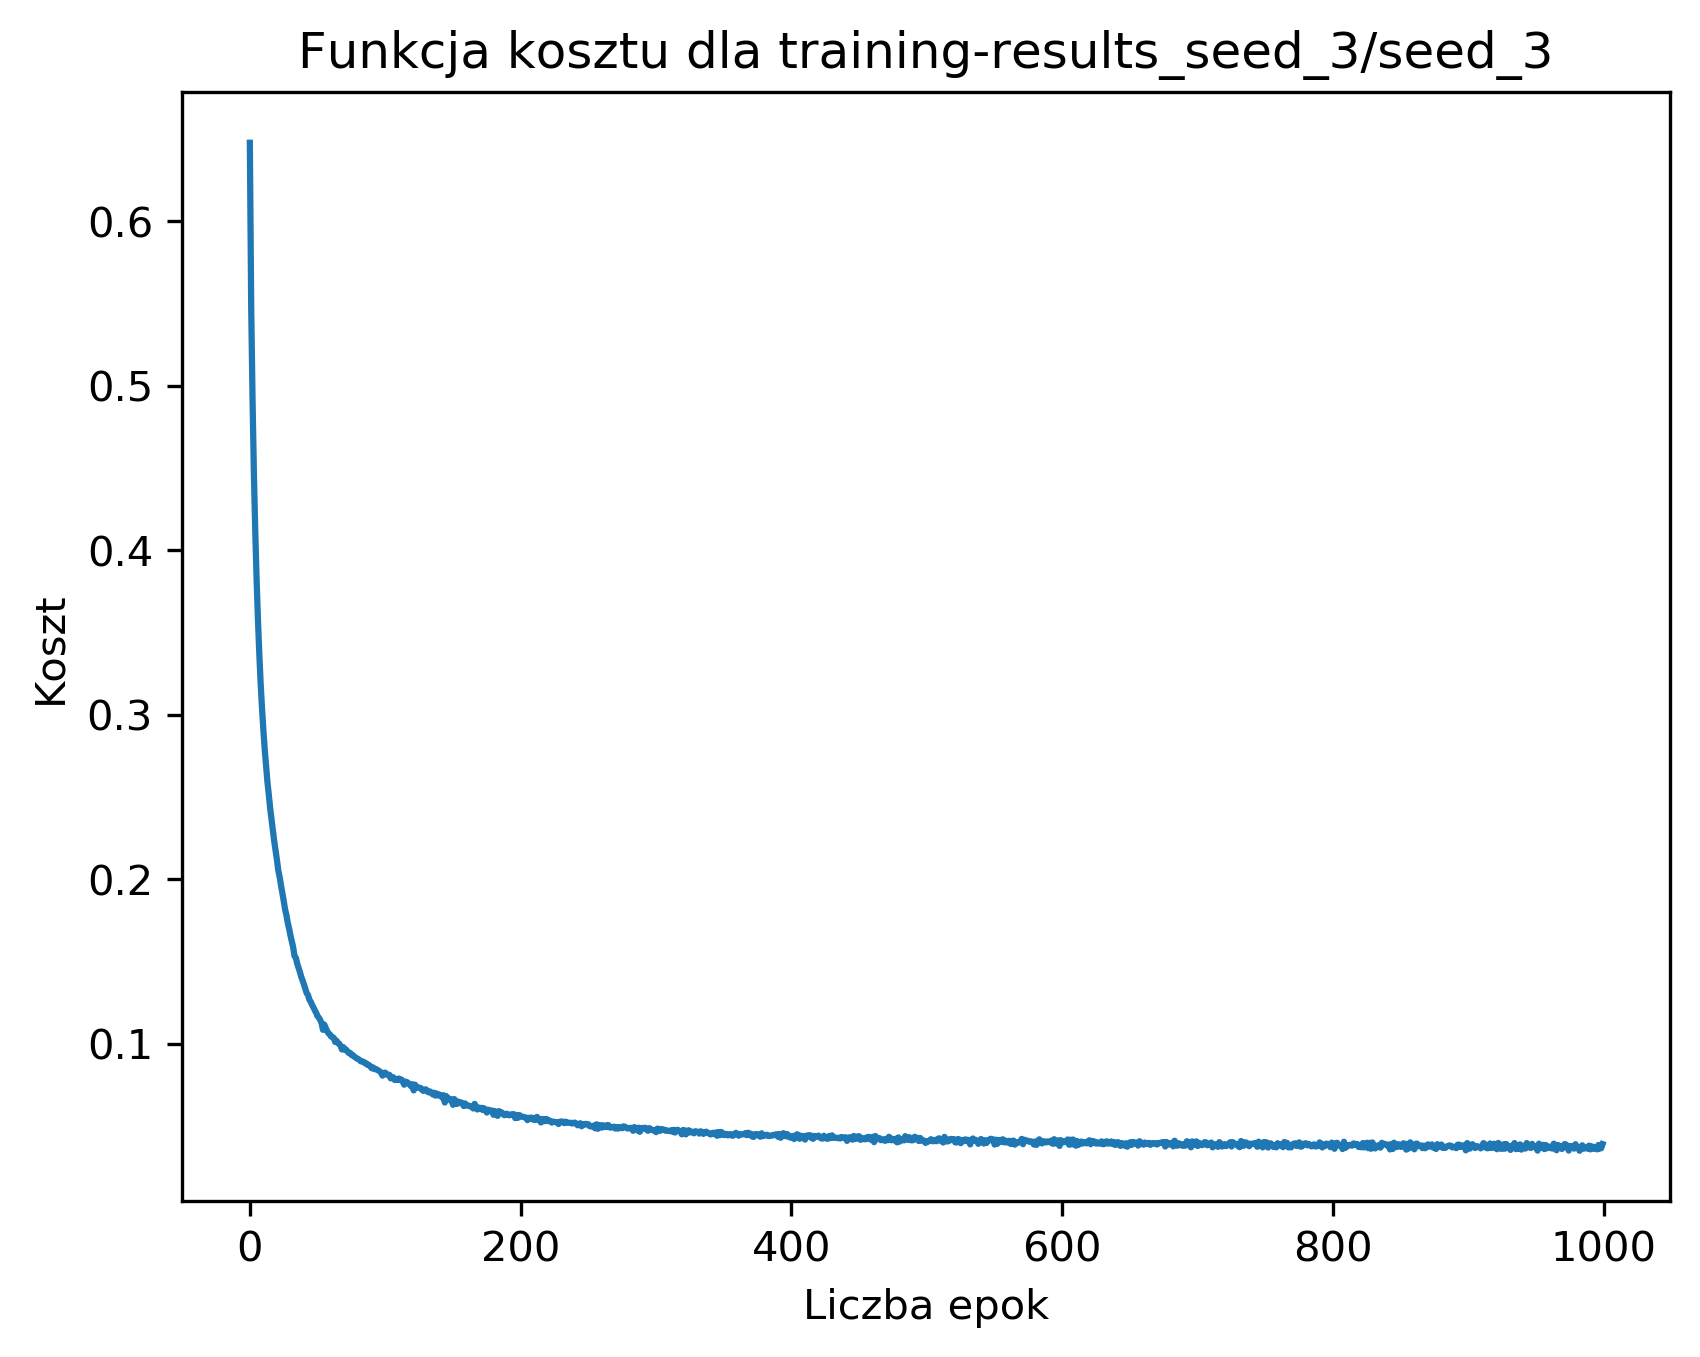
\includegraphics[width=110mm]{wykresy/seed_3_cost.png}
                    \caption{Tryb z standaryzowanymi danymi}
                \end{figure}
                \begin{figure}[!htbp]
                    \centering
                    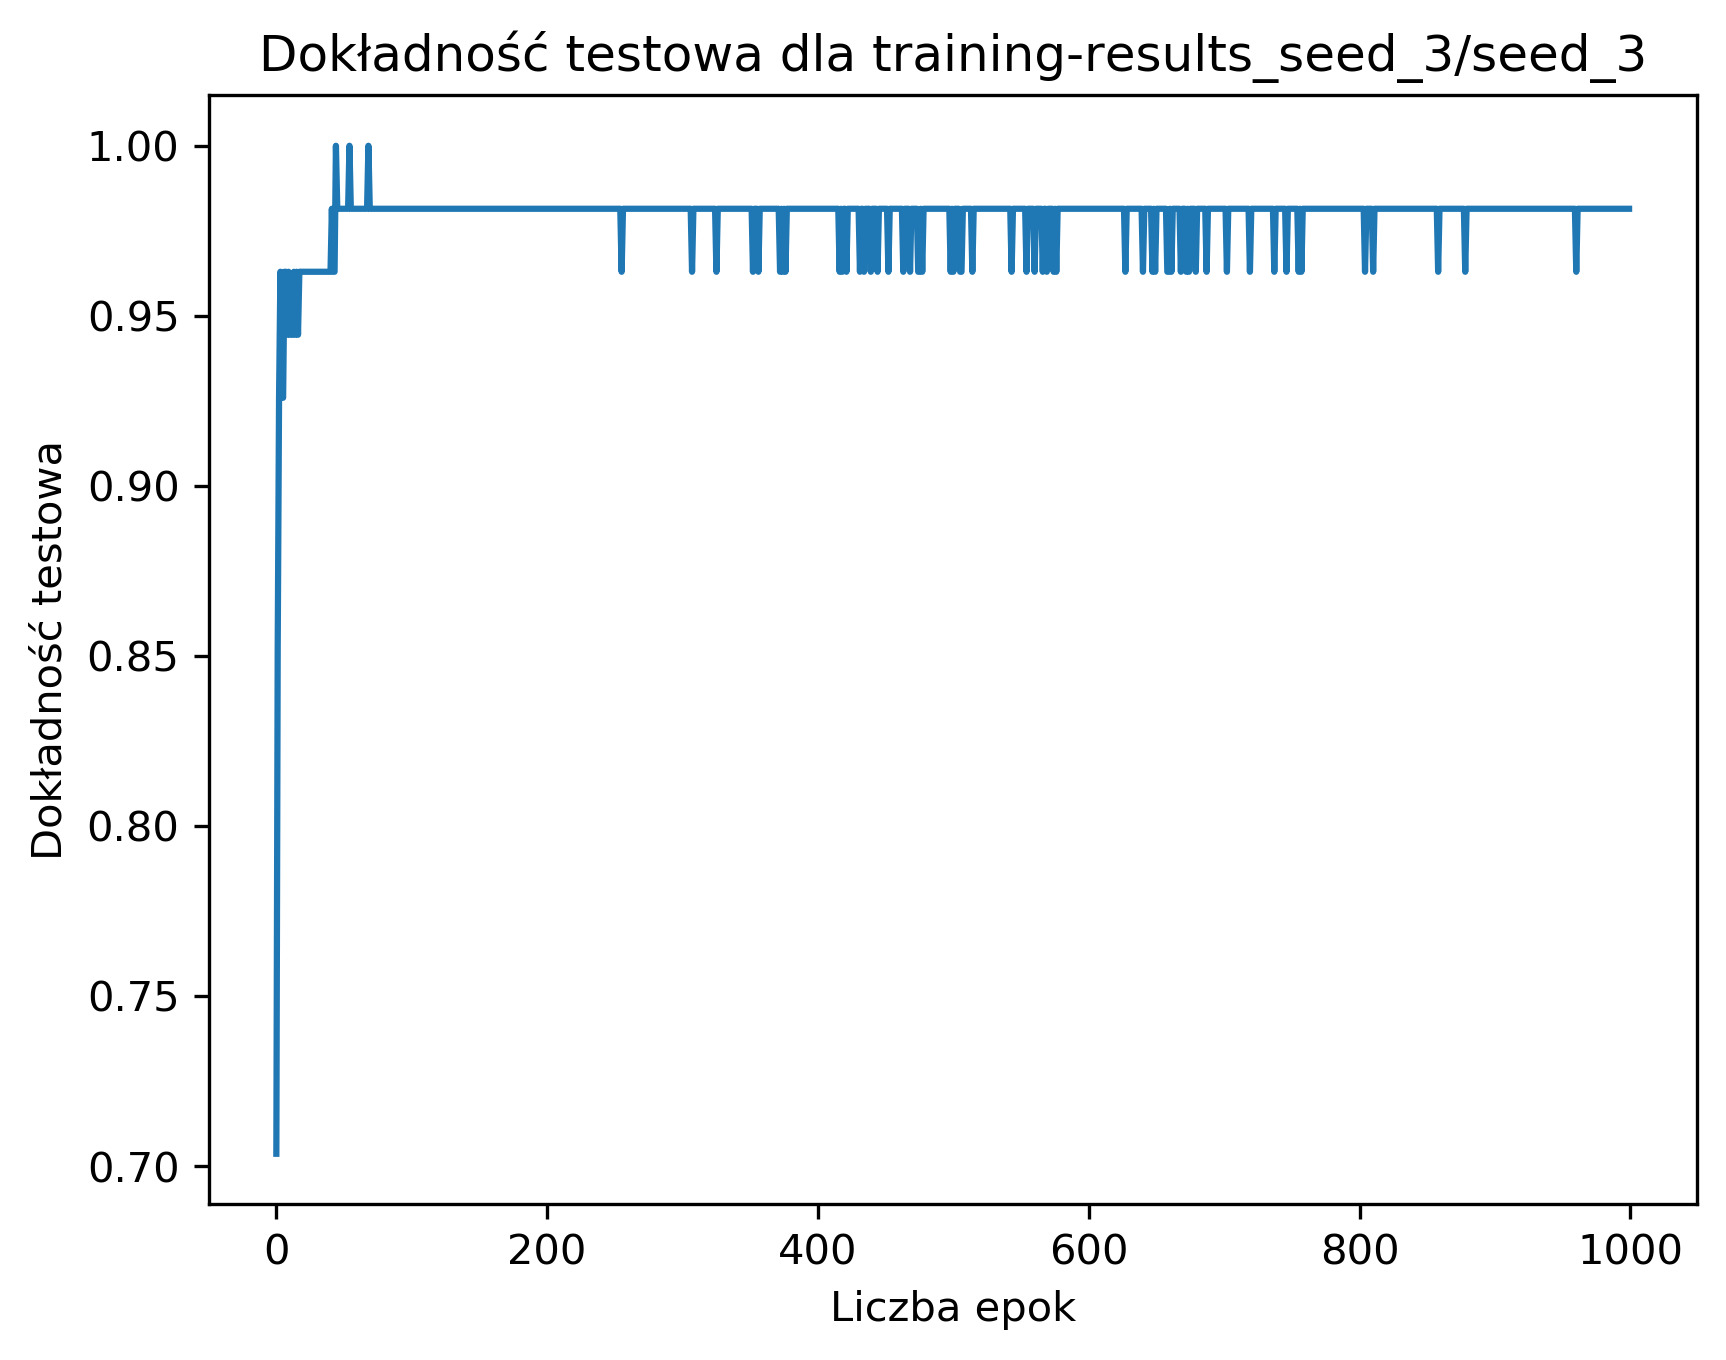
\includegraphics[width=110mm]{wykresy/seed_3_testing-accuracy.png}
                    \caption{Tryb z standaryzowanymi danymi}
                \end{figure}
                \begin{figure}[!htbp]
                    \centering
                    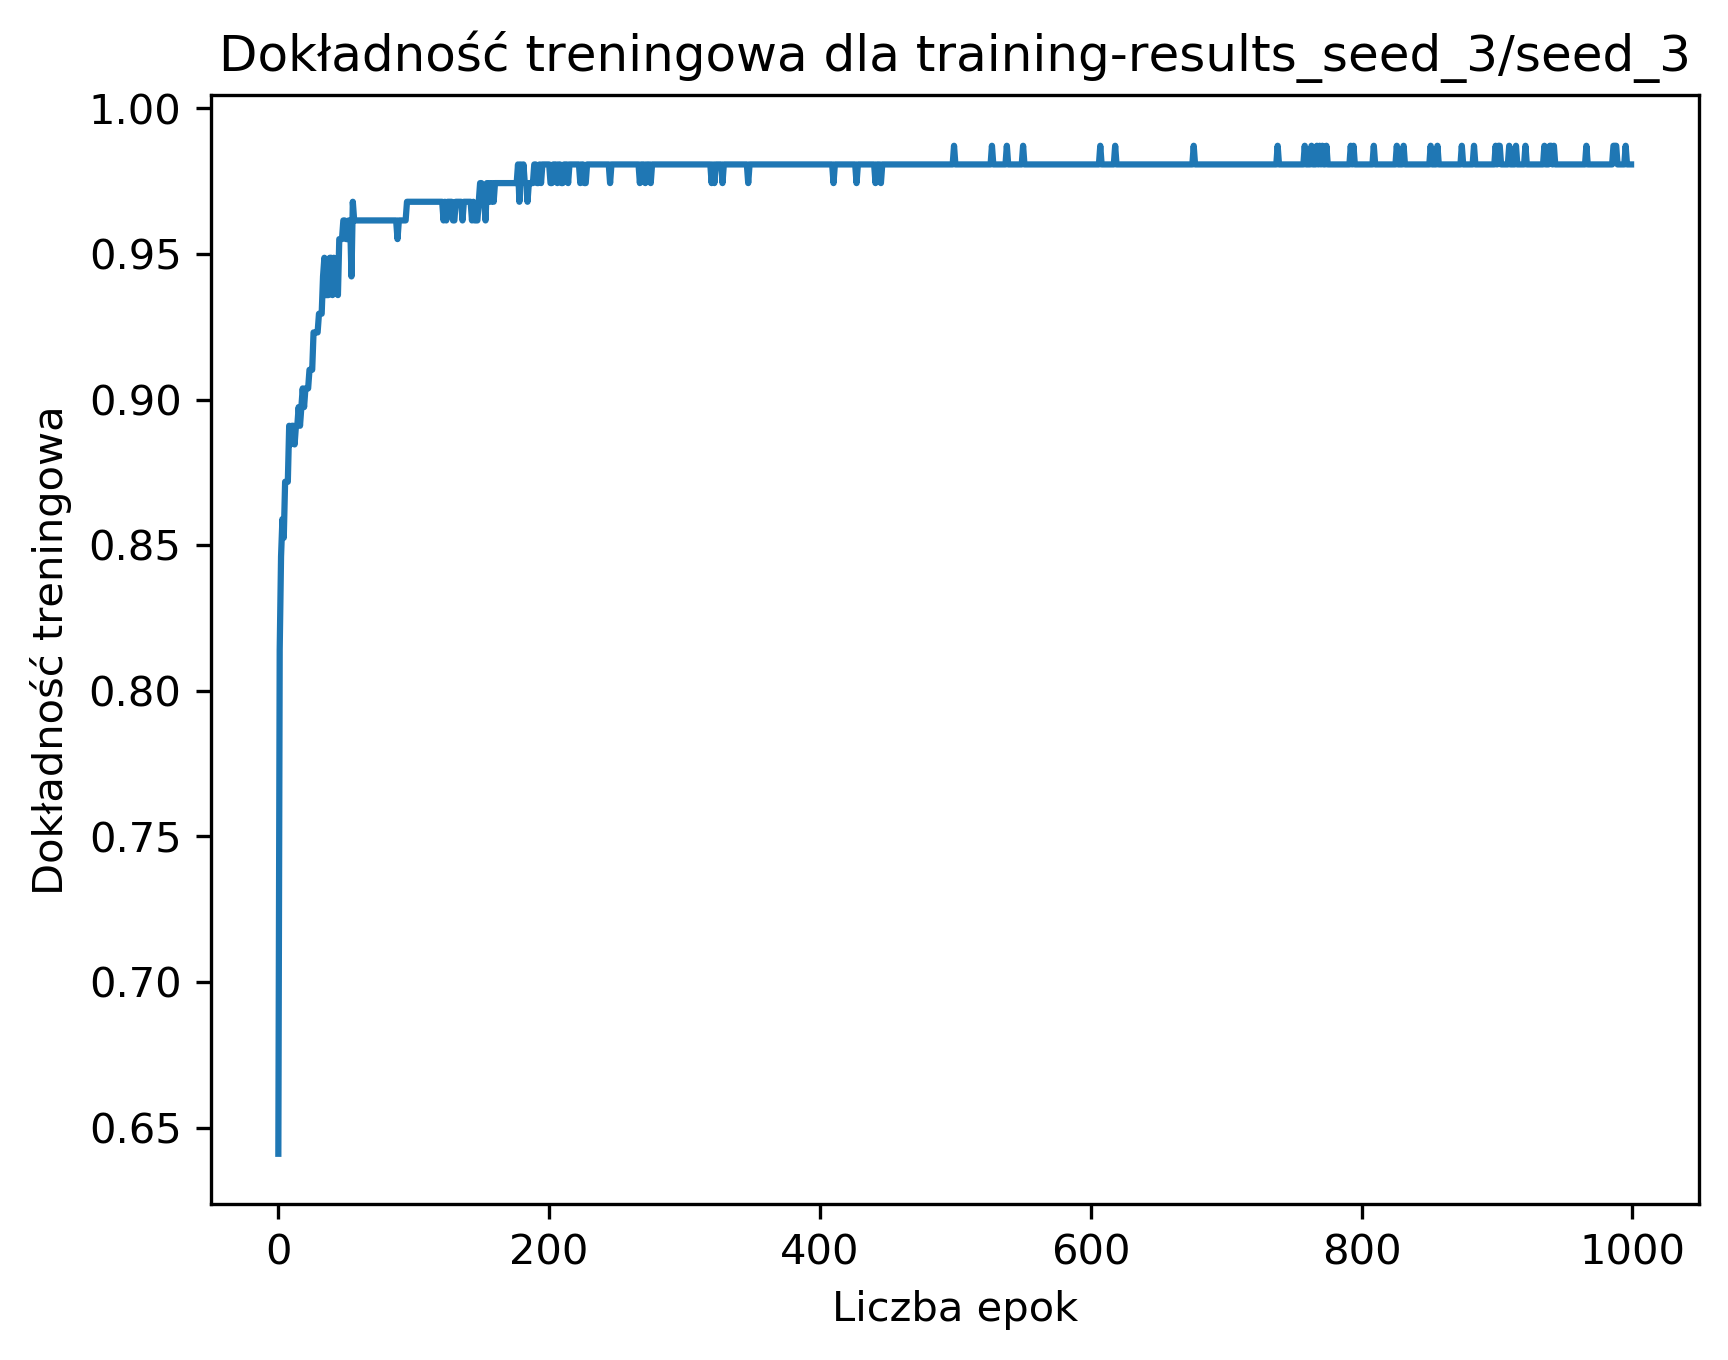
\includegraphics[width=110mm]{wykresy/seed_3_training-accuracy.png}
                    \caption{Tryb z standaryzowanymi danymi}
                \end{figure}
                \FloatBarrier
            %---------------------------------------------------%
                \textbf{Tablice pomyłem}
                \begin{lstlisting}
>> ./data/seeds-standardised-train.csv

> Global confusion matrix:
                [1]      [2]      [3]
                [1]      52 0 3
                [2]       0 52 0
                [3]       0 0 49


                Total population | 156

                Accuracy | 98.0769 %



                > [1]
                [Positive]    [Negative]
                [Positive]           52 3
                [Negative]            0 101


                Total population | 156

                True positive | 52
                True negative | 101
                False positive (type I error) | 3
                False negative (type II error) | 0

                Predicted positive | 55
                Predicted negative | 101
                Actual positive | 52
                Actual negative | 104

                Positive predictive value | 94.5455 %
                False discovery rate | 5.45455 %
                False omission rate | 0 %
                Negative prediction value | 100 %

                True positive rate | 100 %
                False positive rate | 5.76923 %
                False negative rate | 0 %
                True negative rate | 97.1154 %

                Accuracy | 98.0769 %



                > [2]
                [Positive]    [Negative]
                [Positive]           52 0
                [Negative]            0 104


                Total population | 156

                True positive | 52
                True negative | 104
                False positive (type I error) | 0
                False negative (type II error) | 0

                Predicted positive | 52
                Predicted negative | 104
                Actual positive | 52
                Actual negative | 104

                Positive predictive value | 100 %
                False discovery rate | 0 %
                False omission rate | 0 %
                Negative prediction value | 100 %

                True positive rate | 100 %
                False positive rate | 0 %
                False negative rate | 0 %
                True negative rate | 100 %

                Accuracy | 100 %



                > [3]
                [Positive]    [Negative]
                [Positive]           49 0
                [Negative]            3 104


                Total population | 156

                True positive | 49
                True negative | 104
                False positive (type I error) | 0
                False negative (type II error) | 3

                Predicted positive | 49
                Predicted negative | 107
                Actual positive | 52
                Actual negative | 104

                Positive predictive value | 100 %
                False discovery rate | 0 %
                False omission rate | 2.80374 %
                Negative prediction value | 97.1963 %

                True positive rate | 94.2308 %
                False positive rate | 0 %
                False negative rate | 2.88462 %
                True negative rate | 100 %

                Accuracy | 98.0769 %


                >> ./data/seeds-standardised-test.csv

                > Global confusion matrix:
                [1]      [2]      [3]
                [1]      18 0 1
                [2]       0 18 0
                [3]       0 0 17


                Total population | 54

                Accuracy | 98.1481 %



                > [1]
                [Positive]    [Negative]
                [Positive]           18 1
                [Negative]            0 35


                Total population | 54

                True positive | 18
                True negative | 35
                False positive (type I error) | 1
                False negative (type II error) | 0

                Predicted positive | 19
                Predicted negative | 35
                Actual positive | 18
                Actual negative | 36

                Positive predictive value | 94.7368 %
                False discovery rate | 5.26316 %
                False omission rate | 0 %
                Negative prediction value | 100 %

                True positive rate | 100 %
                False positive rate | 5.55556 %
                False negative rate | 0 %
                True negative rate | 97.2222 %

                Accuracy | 98.1481 %



                > [2]
                [Positive]    [Negative]
                [Positive]           18 0
                [Negative]            0 36


                Total population | 54

                True positive | 18
                True negative | 36
                False positive (type I error) | 0
                False negative (type II error) | 0

                Predicted positive | 18
                Predicted negative | 36
                Actual positive | 18
                Actual negative | 36

                Positive predictive value | 100 %
                False discovery rate | 0 %
                False omission rate | 0 %
                Negative prediction value | 100 %

                True positive rate | 100 %
                False positive rate | 0 %
                False negative rate | 0 %
                True negative rate | 100 %

                Accuracy | 100 %



                > [3]
                [Positive]    [Negative]
                [Positive]           17 0
                [Negative]            1 36


                Total population | 54

                True positive | 17
                True negative | 36
                False positive (type I error) | 0
                False negative (type II error) | 1

                Predicted positive | 17
                Predicted negative | 37
                Actual positive | 18
                Actual negative | 36

                Positive predictive value | 100 %
                False discovery rate | 0 %
                False omission rate | 2.7027 %
                Negative prediction value | 97.2973 %

                True positive rate | 94.4444 %
                False positive rate | 0 %
                False negative rate | 2.77778 %
                True negative rate | 100 %

                Accuracy | 98.1481 %
                \end{lstlisting}
            %---------------------------------------------------%
            }
        %---------------------------------------------------%
            \subsubsection{K najbliższych sąsiadów}
            {
                \textbf{Tryb danych domyślny, wartość K = 5}
                \begin{lstlisting}
>> ./data/seeds-test.csv

> Global confusion matrix:
                [1]      [2]      [3]
                [1]      23 0 1
                [2]       3 28 0
                [3]       2 0 27


                Total population | 84

                Accuracy | 92.8571 %



                > [1]
                [Positive]    [Negative]
                [Positive]           23 1
                [Negative]            5 55


                Total population | 84

                True positive | 23
                True negative | 55
                False positive (type I error) | 1
                False negative (type II error) | 5

                Correct positive predictions | 95.8333 %
                Correct negative predictions | 91.6667 %

                Correct positive classifications | 82.1429 %
                Correct negative classifications | 98.2143 %

                Accuracy | 92.8571 %



                > [2]
                [Positive]    [Negative]
                [Positive]           28 3
                [Negative]            0 53


                Total population | 84

                True positive | 28
                True negative | 53
                False positive (type I error) | 3
                False negative (type II error) | 0

                Correct positive predictions | 90.3226 %
                Correct negative predictions | 100 %

                Correct positive classifications | 100 %
                Correct negative classifications | 94.6429 %

                Accuracy | 96.4286 %



                > [3]
                [Positive]    [Negative]
                [Positive]           27 2
                [Negative]            1 54


                Total population | 84

                True positive | 27
                True negative | 54
                False positive (type I error) | 2
                False negative (type II error) | 1

                Correct positive predictions | 93.1034 %
                Correct negative predictions | 98.1818 %

                Correct positive classifications | 96.4286 %
                Correct negative classifications | 96.4286 %

                Accuracy | 96.4286 %

                \end{lstlisting}
            %---------------------------------------------------%
                \textbf{Tryb z normalizowanymi danymi, wartość K = 5}
                \begin{lstlisting}
>> ./data/seeds-normalised-test.csv

> Global confusion matrix:
                [1]      [2]      [3]
                [1]      25 0 0
                [2]       2 28 0
                [3]       1 0 28


                Total population | 84

                Accuracy | 96.4286 %



                > [1]
                [Positive]    [Negative]
                [Positive]           25 0
                [Negative]            3 56


                Total population | 84

                True positive | 25
                True negative | 56
                False positive (type I error) | 0
                False negative (type II error) | 3

                Correct positive predictions | 100 %
                Correct negative predictions | 94.9153 %

                Correct positive classifications | 89.2857 %
                Correct negative classifications | 100 %

                Accuracy | 96.4286 %



                > [2]
                [Positive]    [Negative]
                [Positive]           28 2
                [Negative]            0 54


                Total population | 84

                True positive | 28
                True negative | 54
                False positive (type I error) | 2
                False negative (type II error) | 0

                Correct positive predictions | 93.3333 %
                Correct negative predictions | 100 %

                Correct positive classifications | 100 %
                Correct negative classifications | 96.4286 %

                Accuracy | 97.619 %



                > [3]
                [Positive]    [Negative]
                [Positive]           28 1
                [Negative]            0 55


                Total population | 84

                True positive | 28
                True negative | 55
                False positive (type I error) | 1
                False negative (type II error) | 0

                Correct positive predictions | 96.5517 %
                Correct negative predictions | 100 %

                Correct positive classifications | 100 %
                Correct negative classifications | 98.2143 %

                Accuracy | 98.8095 %

                \end{lstlisting}
            %---------------------------------------------------%
                \textbf{Tryb z standaryzowanymi danymi, wartość K = 5}
                \begin{lstlisting}
>> ./data/seeds-standardised-test.csv

> Global confusion matrix:
                [1]      [2]      [3]
                [1]      24 0 0
                [2]       2 28 0
                [3]       2 0 28


                Total population | 84

                Accuracy | 95.2381 %



                > [1]
                [Positive]    [Negative]
                [Positive]           24 0
                [Negative]            4 56


                Total population | 84

                True positive | 24
                True negative | 56
                False positive (type I error) | 0
                False negative (type II error) | 4

                Correct positive predictions | 100 %
                Correct negative predictions | 93.3333 %

                Correct positive classifications | 85.7143 %
                Correct negative classifications | 100 %

                Accuracy | 95.2381 %



                > [2]
                [Positive]    [Negative]
                [Positive]           28 2
                [Negative]            0 54


                Total population | 84

                True positive | 28
                True negative | 54
                False positive (type I error) | 2
                False negative (type II error) | 0

                Correct positive predictions | 93.3333 %
                Correct negative predictions | 100 %

                Correct positive classifications | 100 %
                Correct negative classifications | 96.4286 %

                Accuracy | 97.619 %



                > [3]
                [Positive]    [Negative]
                [Positive]           28 2
                [Negative]            0 54


                Total population | 84

                True positive | 28
                True negative | 54
                False positive (type I error) | 2
                False negative (type II error) | 0

                Correct positive predictions | 93.3333 %
                Correct negative predictions | 100 %

                Correct positive classifications | 100 %
                Correct negative classifications | 96.4286 %

                Accuracy | 97.619 %

                \end{lstlisting}
            %---------------------------------------------------%
            }
        }
    %---------------------------------------------------%
        \subsection{Obrazy - Rozpoznawanie Liczb}
        {
            \subsubsection{Perceptron wielowarstwowy}
            {
                \textbf{Domyślne dane 128}
                \begin{figure}[!htbp]
                    \centering
                    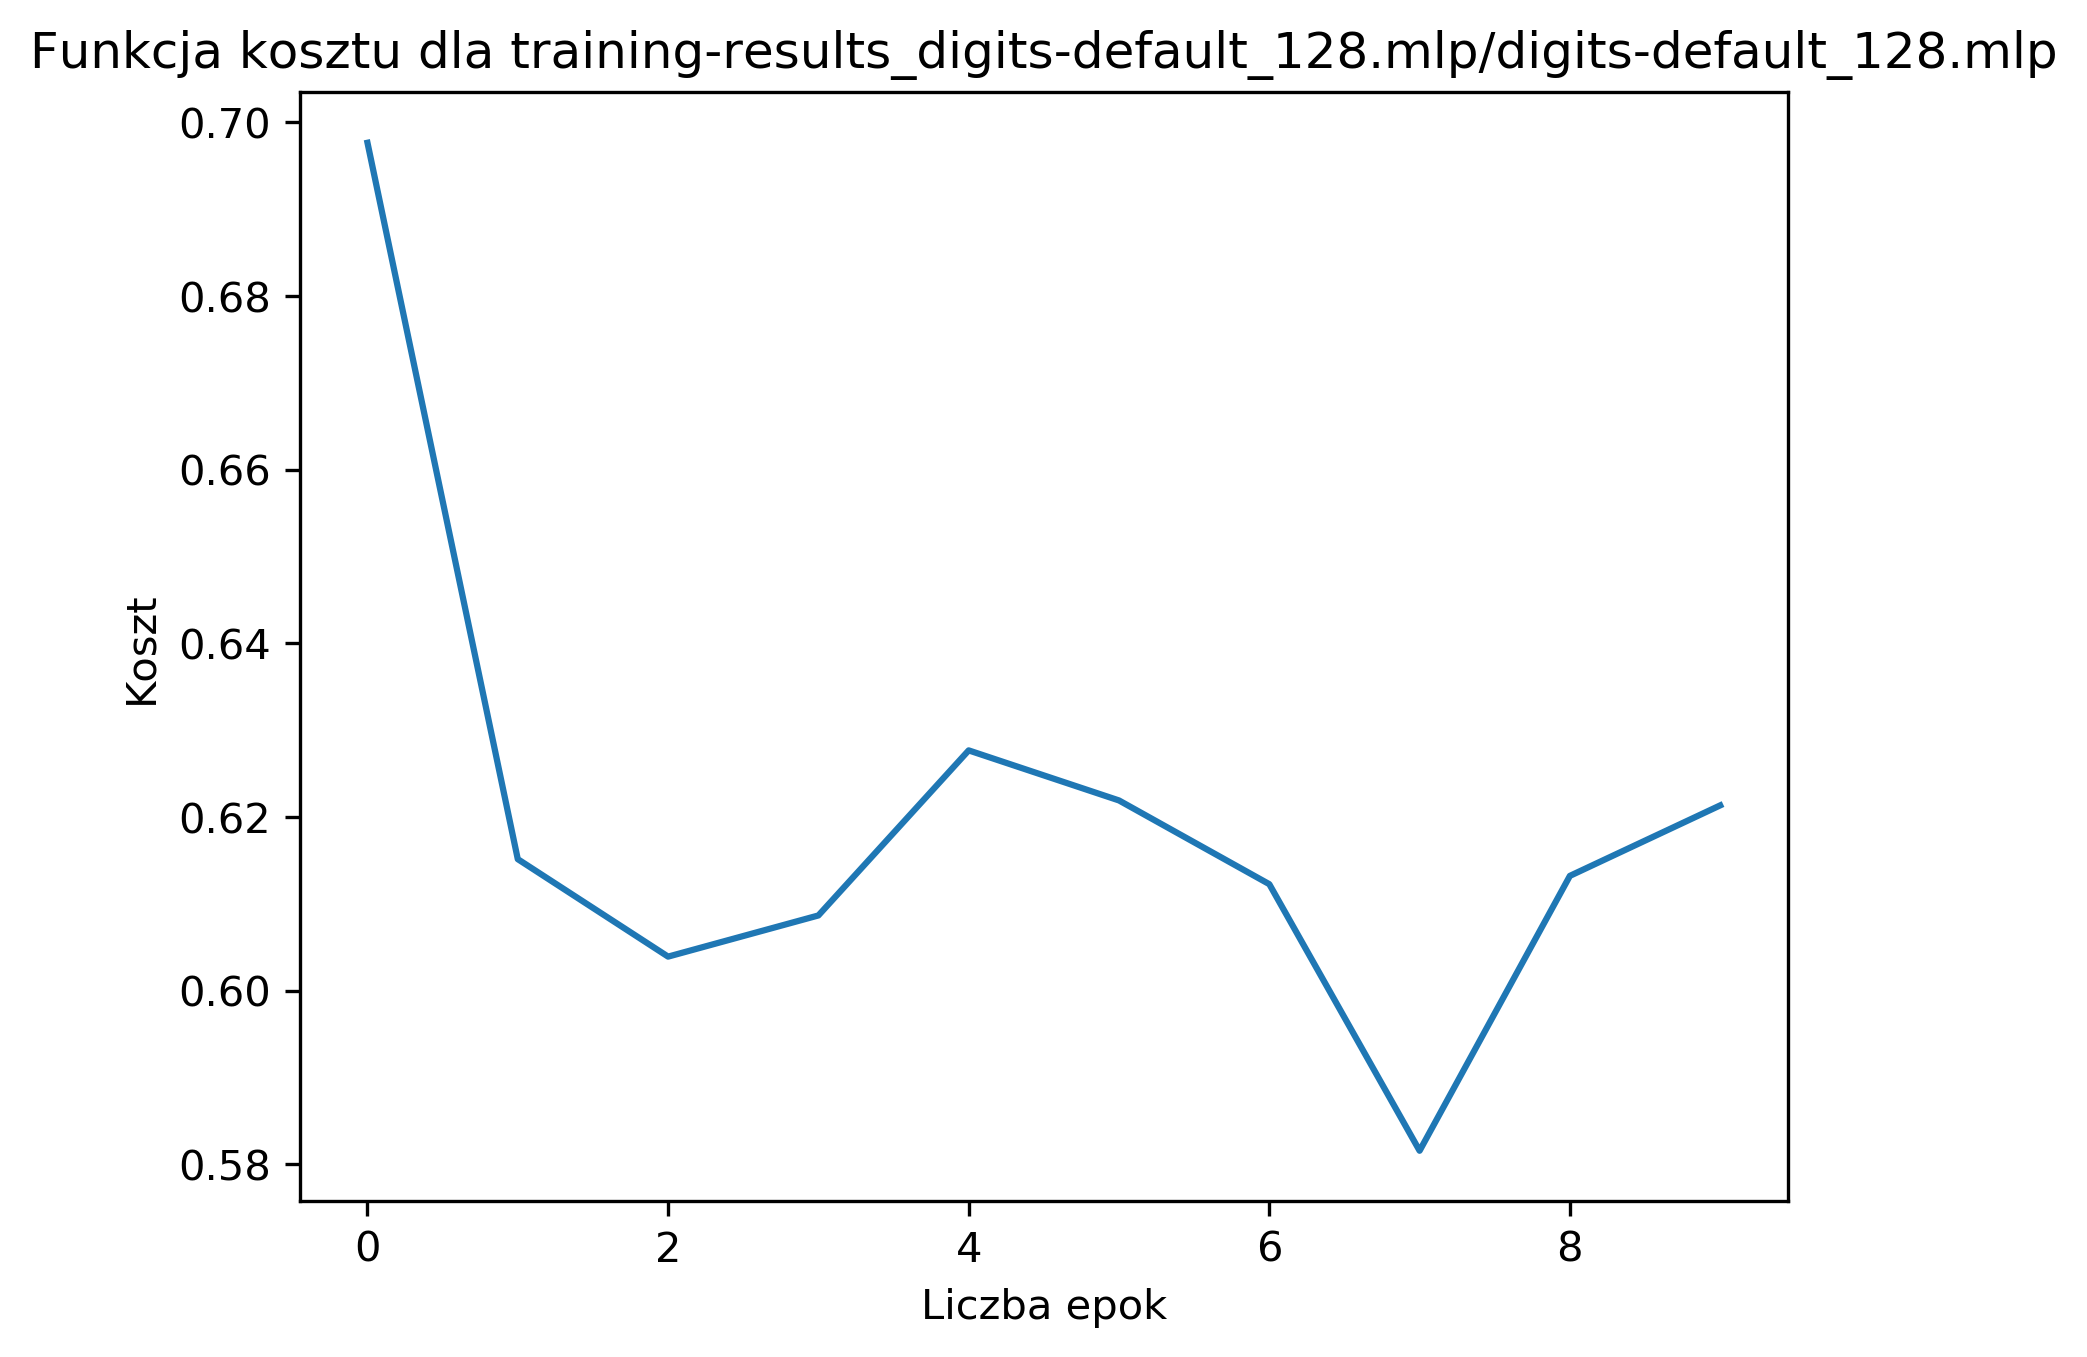
\includegraphics[width=145mm]{wykresy/digits-default_128_mlp_cost.png}
                    \caption{Tryb z domyślnymi danymi}
                \end{figure}
                \begin{figure}[!htbp]
                    \centering
                    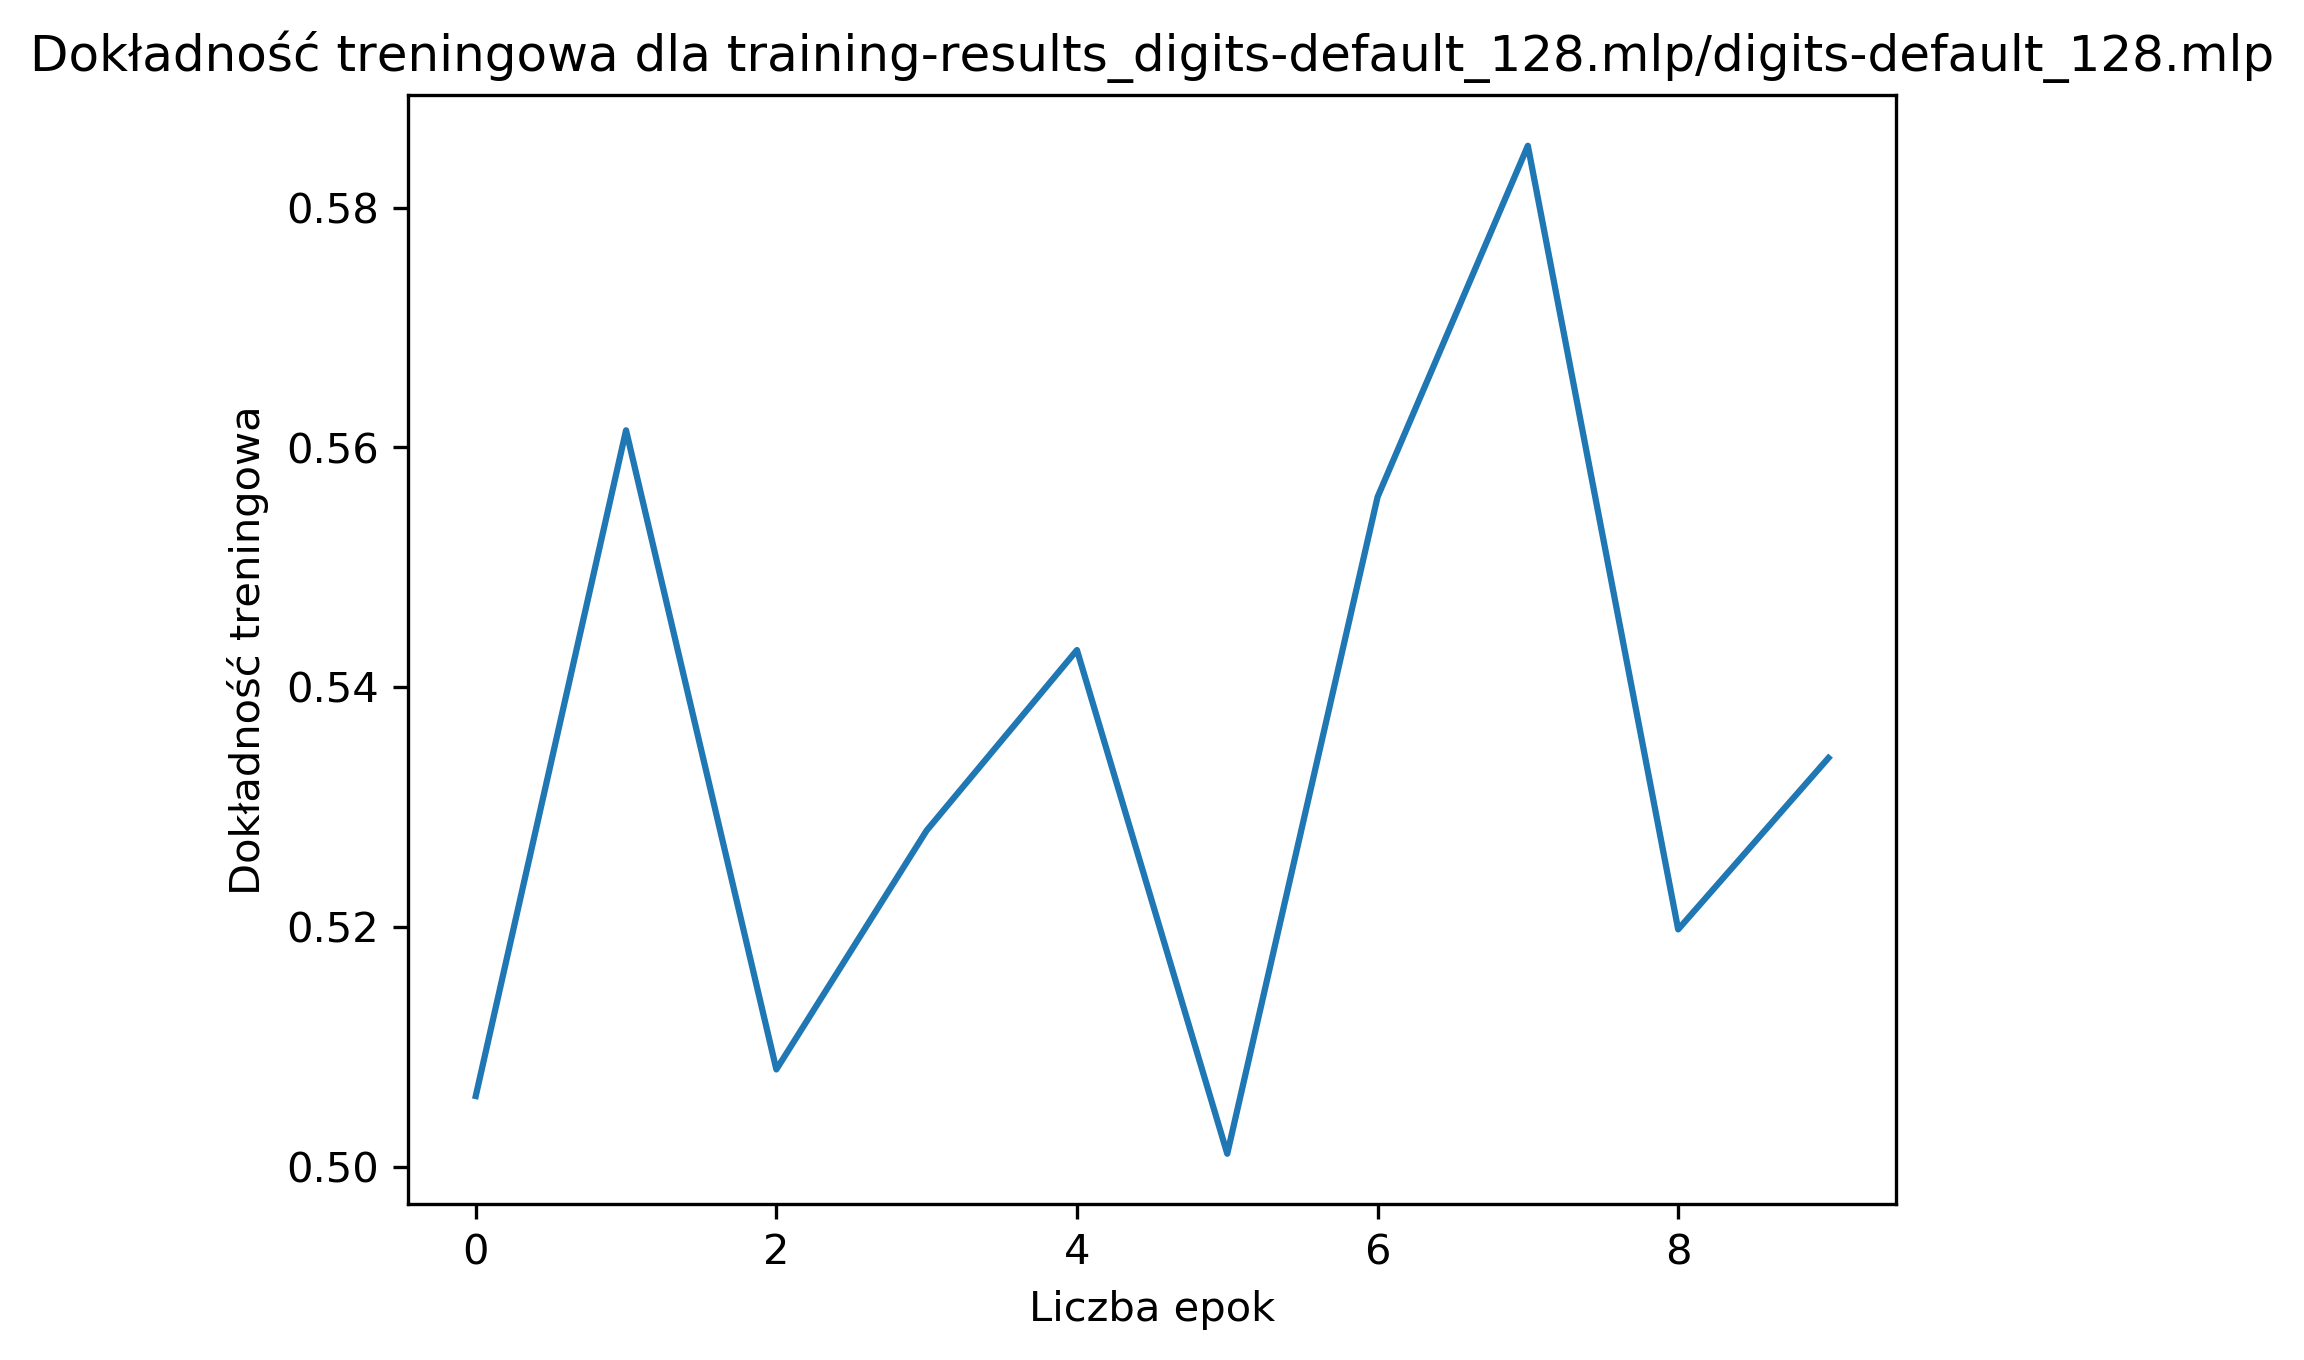
\includegraphics[width=155mm]{wykresy/digits-default_128_mlp_training-accuracy.png}
                    \caption{Tryb z domyślnymi danymi}
                \end{figure}
                \begin{figure}[!htbp]
                    \centering
                    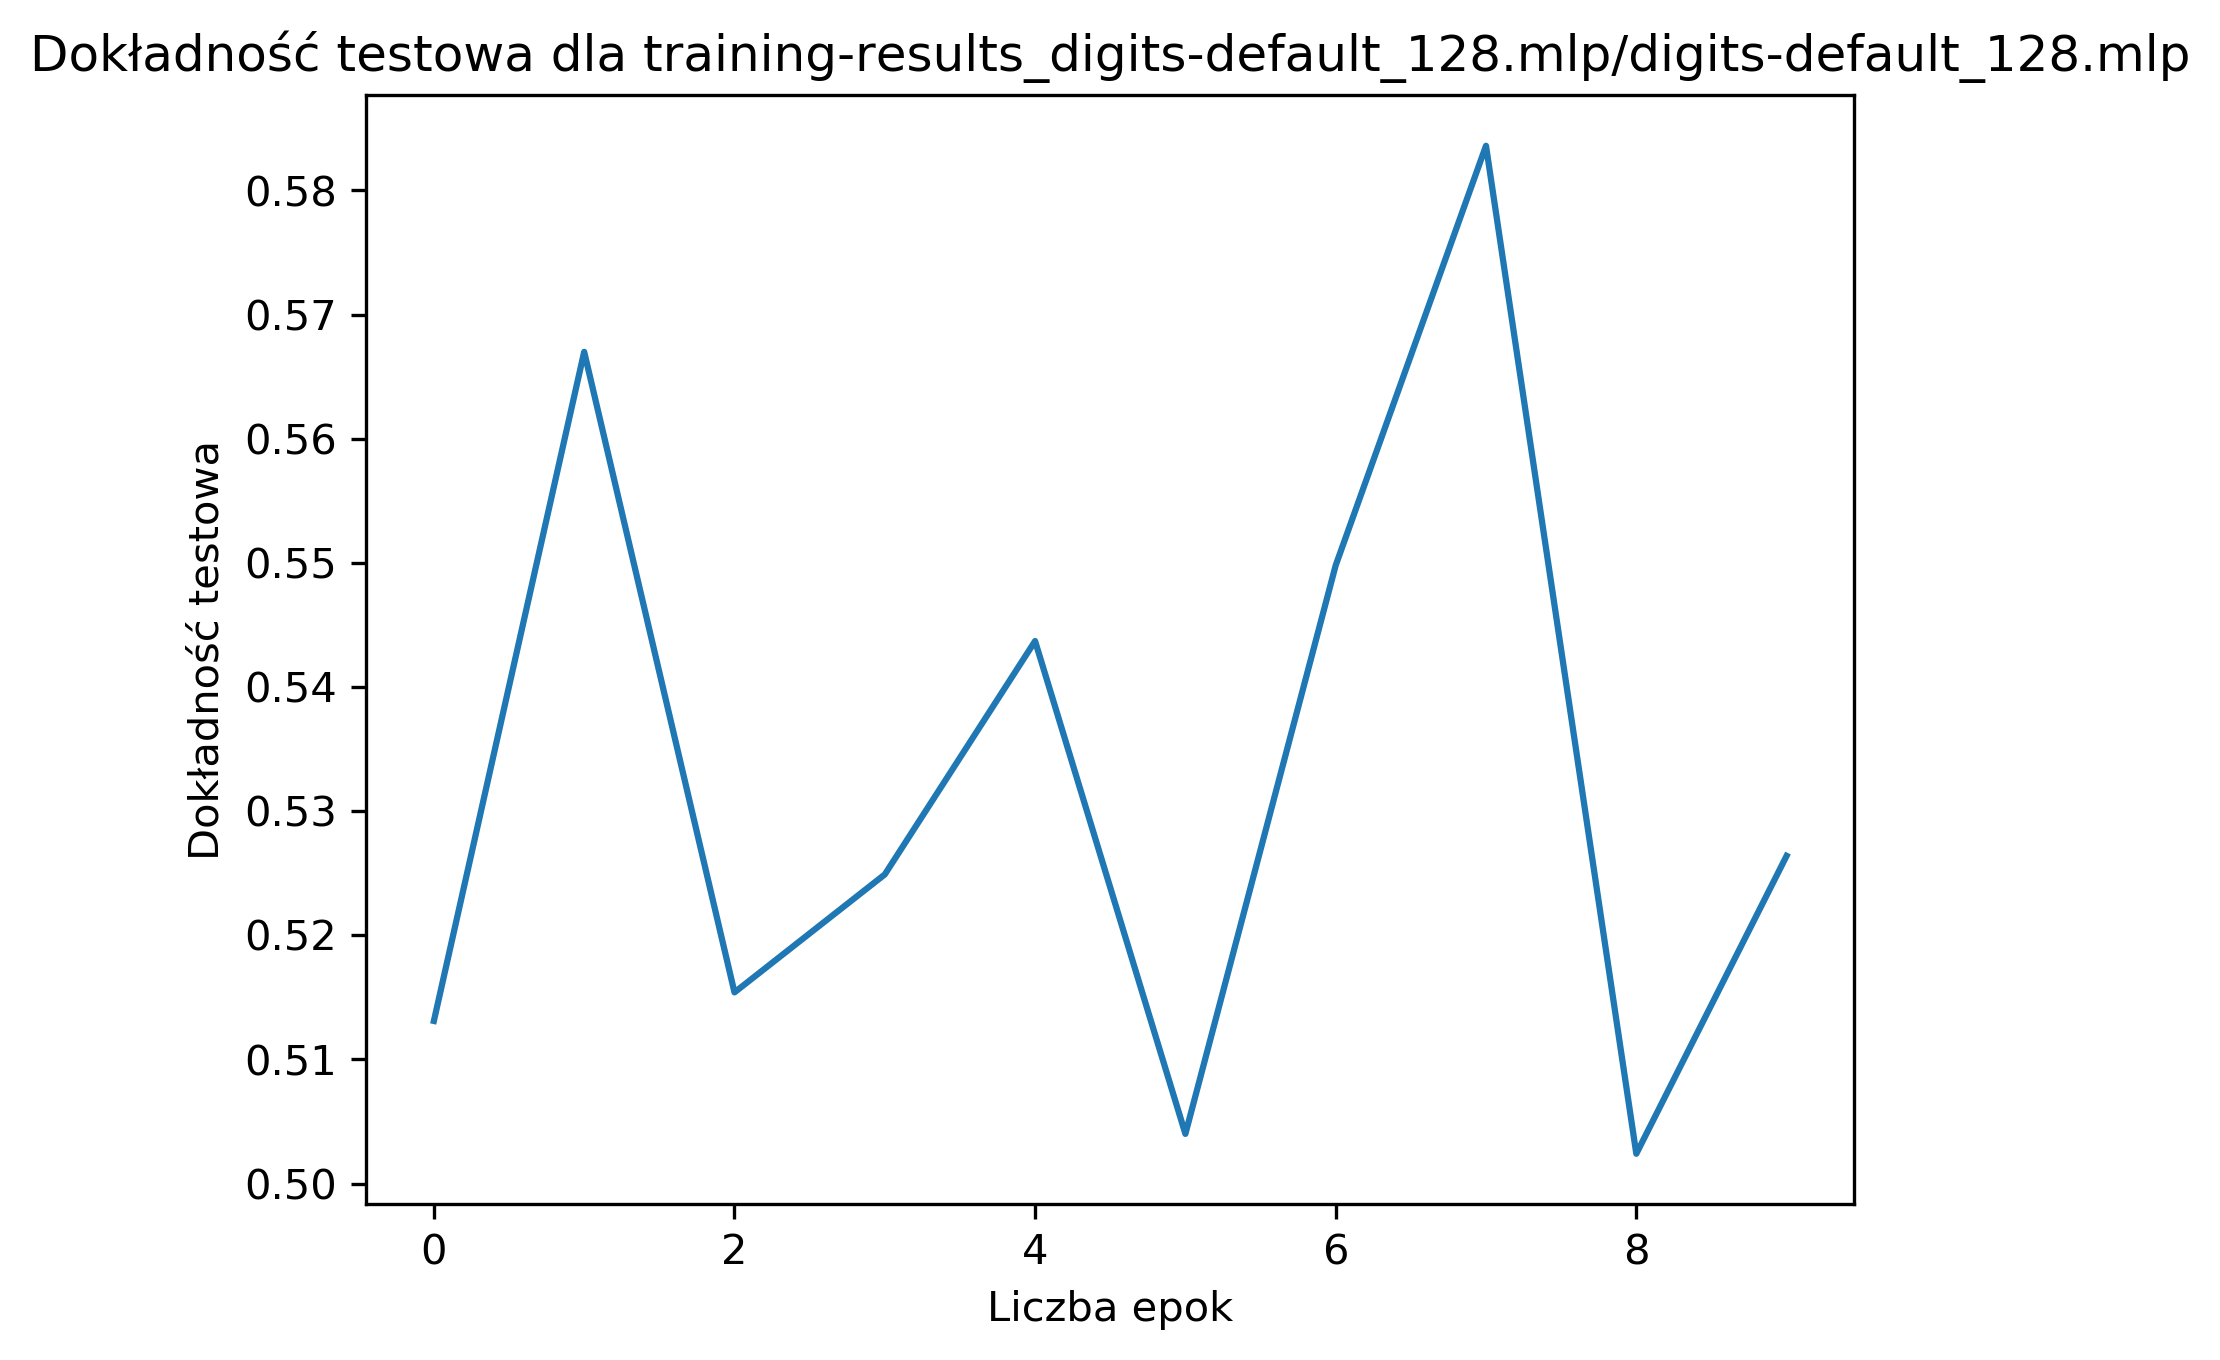
\includegraphics[width=155mm]{wykresy/digits-default_128_mlp_testing-accuracy.png}
                    \caption{Tryb z domyślnymi danymi}
                \end{figure}
                \FloatBarrier
            %---------------------------------------------------%
                \textbf{Histogram gradientu 8}
                \begin{figure}[!htbp]
                    \centering
                    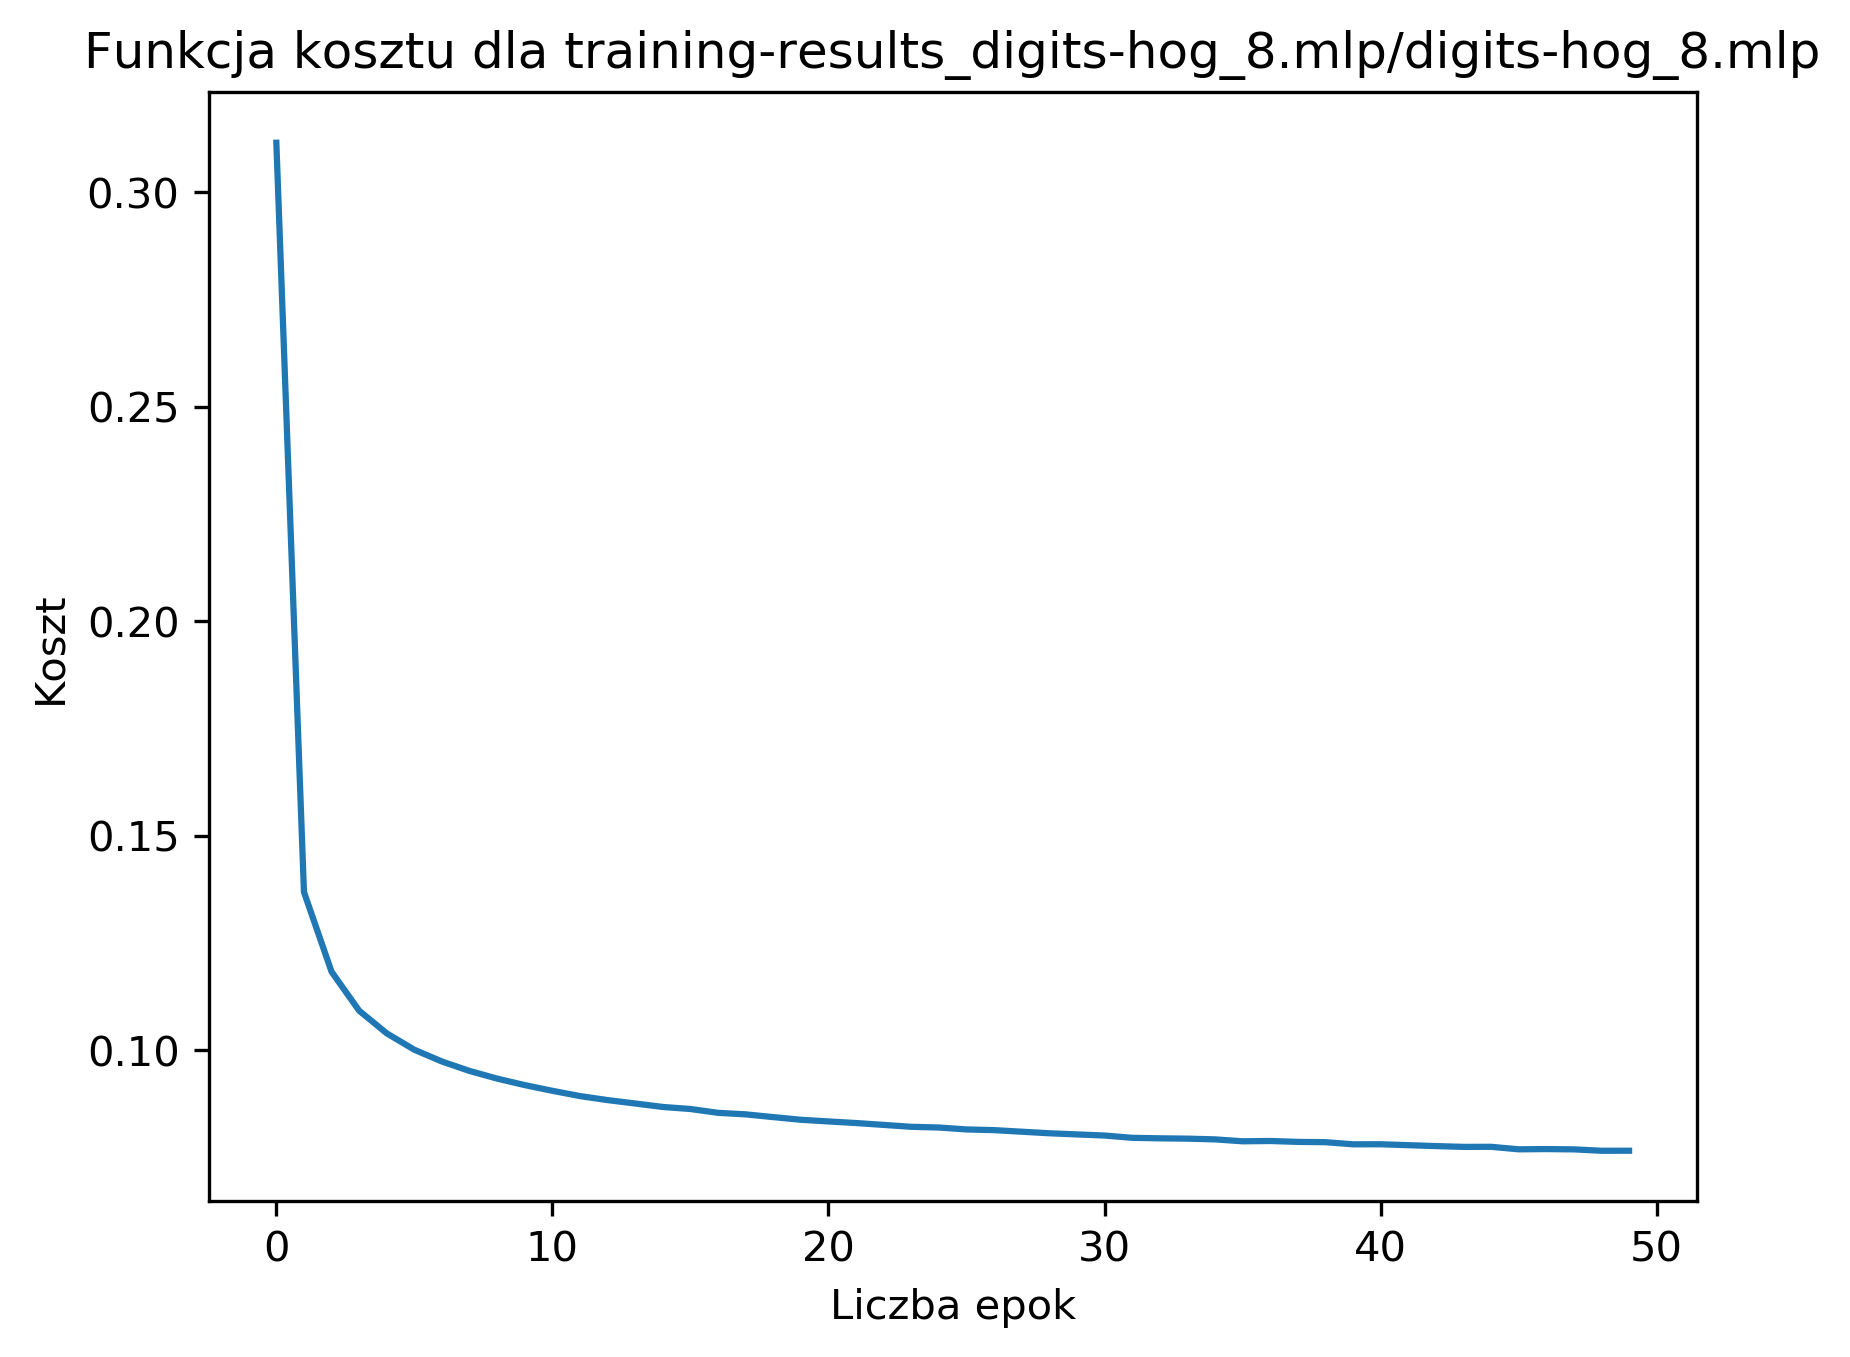
\includegraphics[width=135mm]{wykresy/digits-hog_8_mlp_cost.png}
                    \caption{Tryb z standaryzowanymi danymi}
                \end{figure}
                \begin{figure}[!htbp]
                    \centering
                    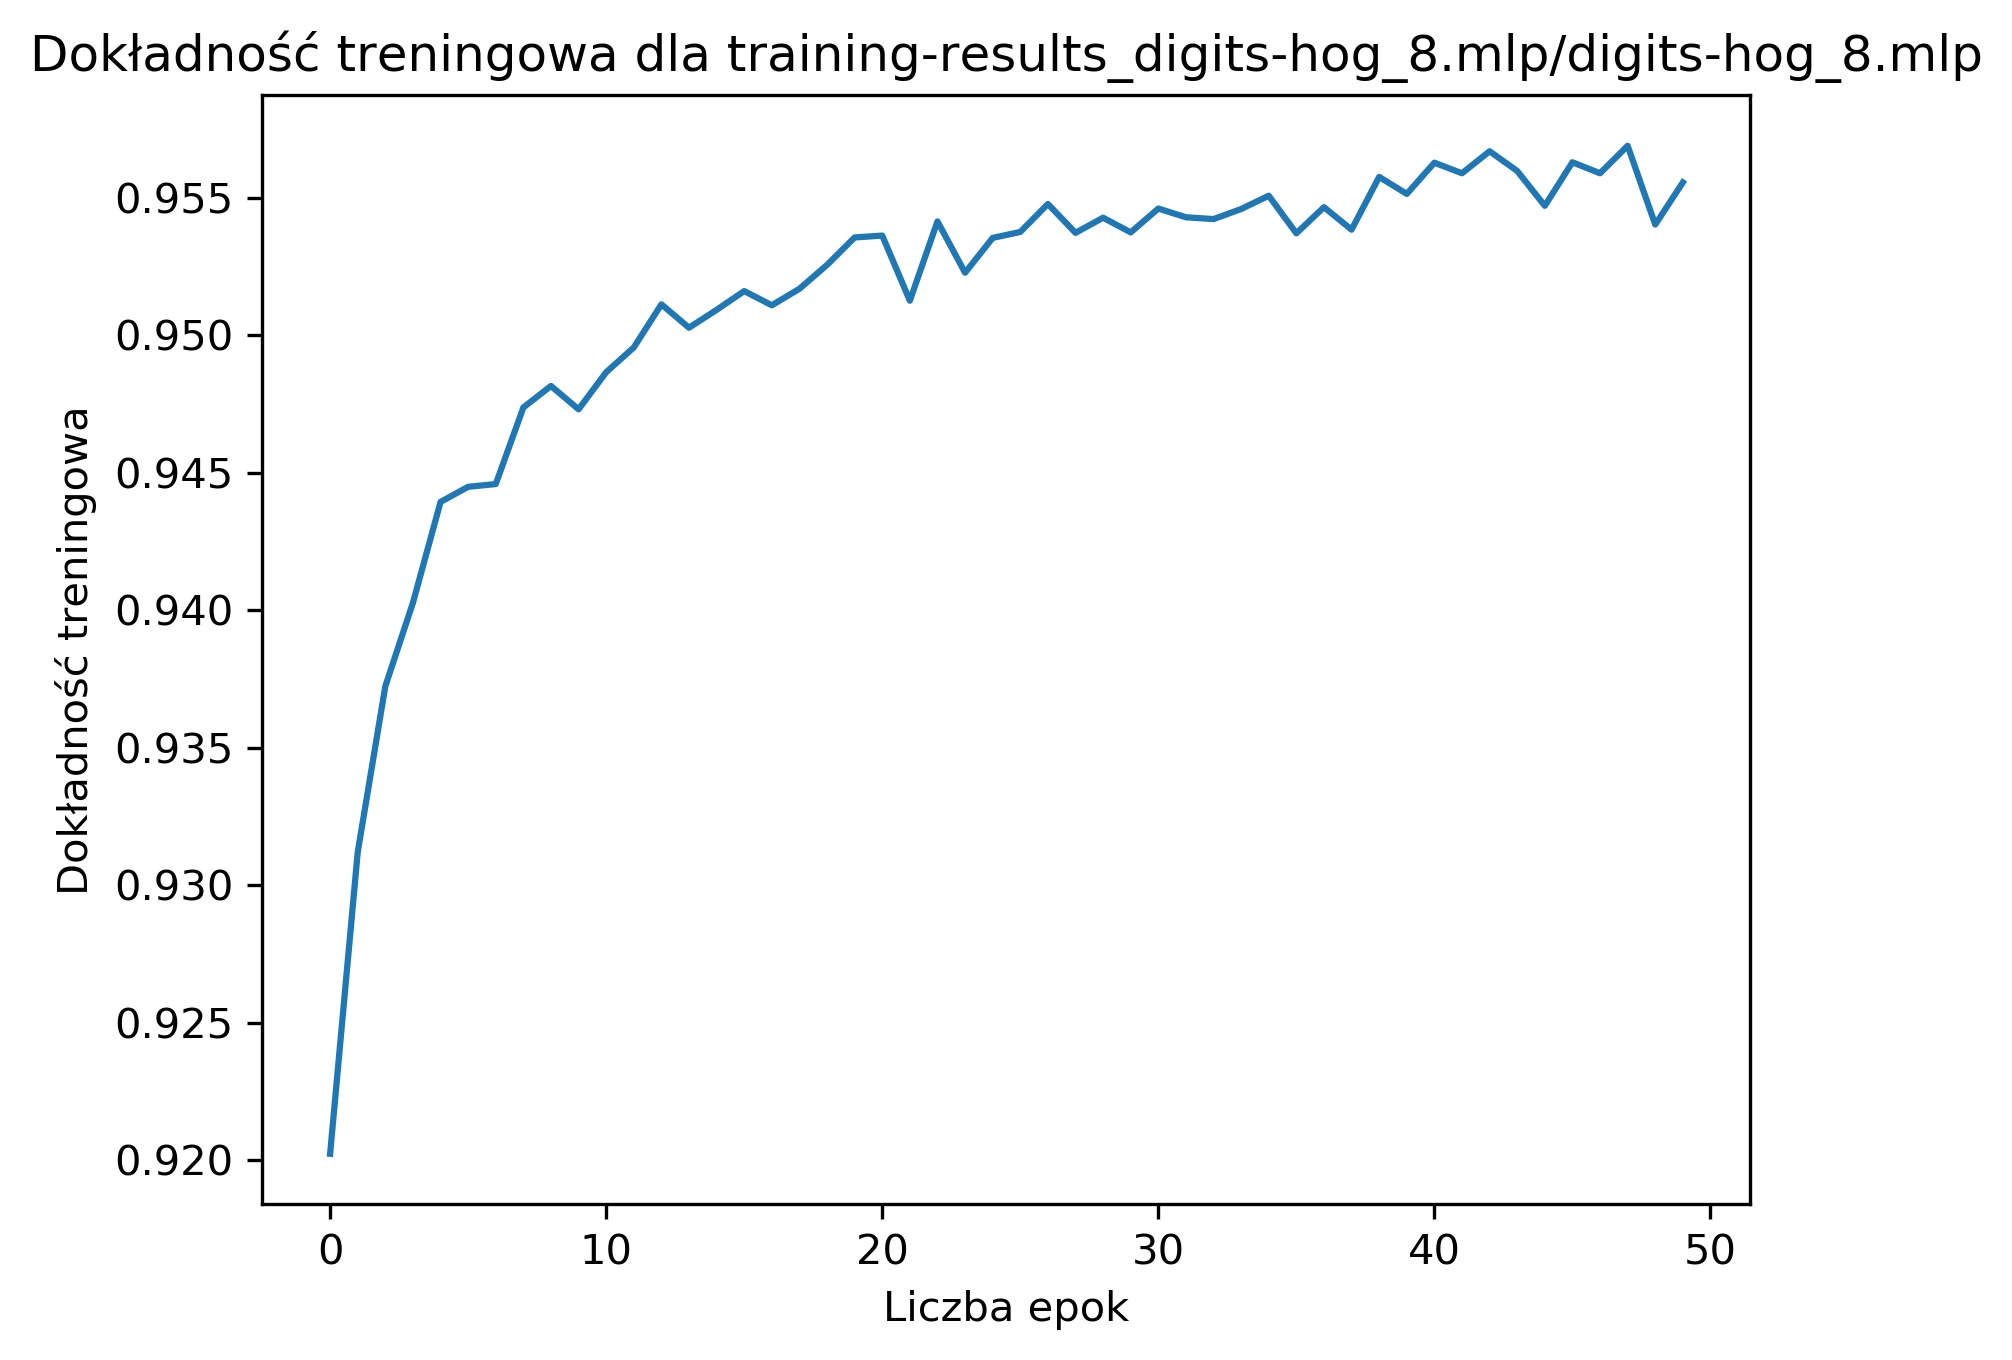
\includegraphics[width=145mm]{wykresy/digits-hog_8_mlp_training-accuracy.png}
                    \caption{Tryb z standaryzowanymi danymi}
                \end{figure}
                \begin{figure}[!htbp]
                    \centering
                    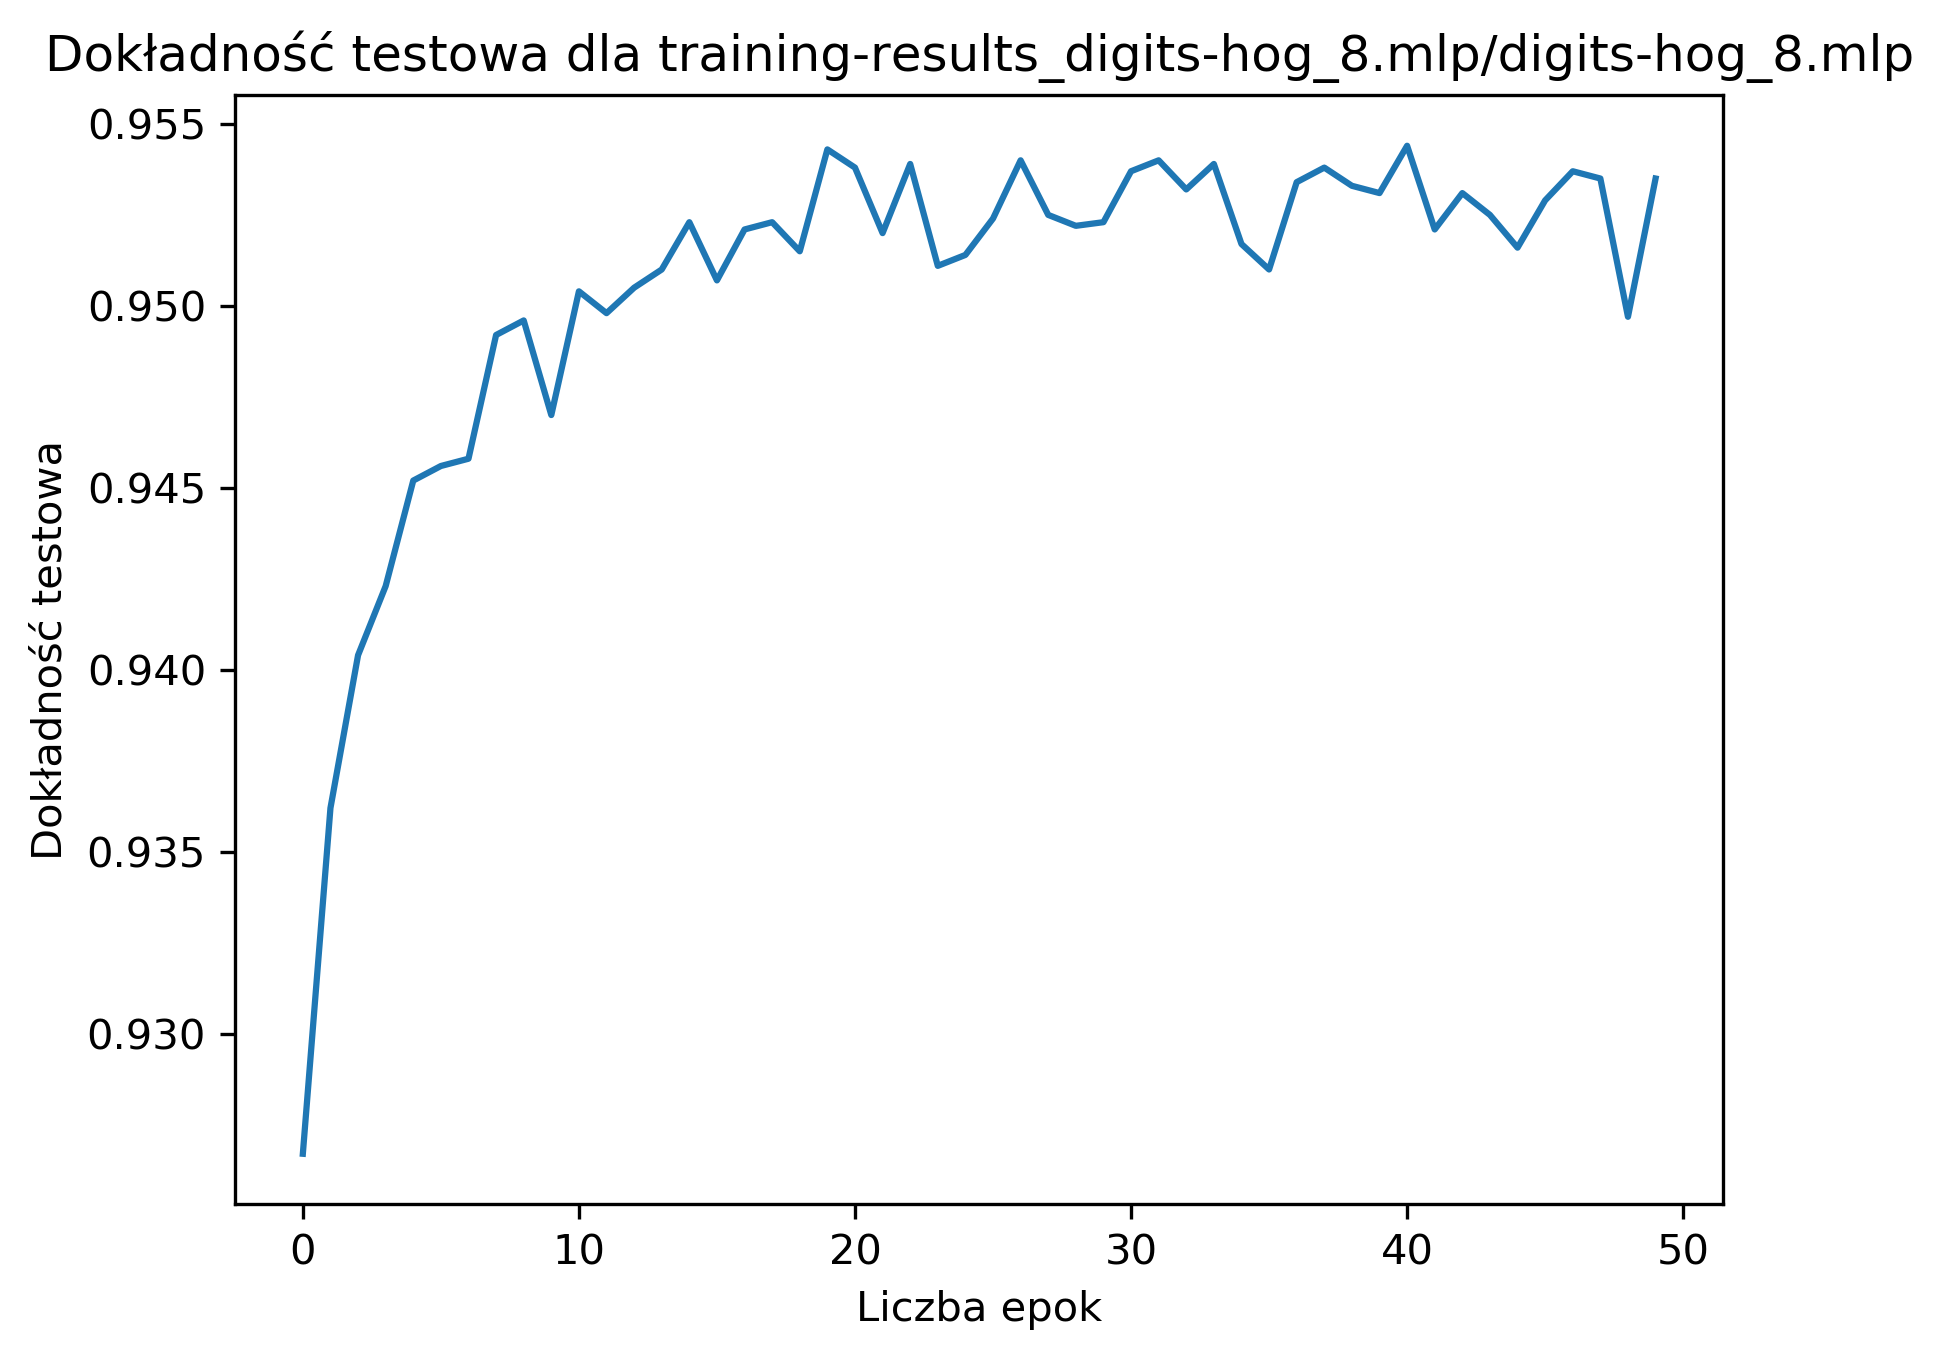
\includegraphics[width=145mm]{wykresy/digits-hog_8_mlp_testing-accuracy.png}
                    \caption{Tryb z standaryzowanymi danymi}
                \end{figure}
                \FloatBarrier
            %---------------------------------------------------%
                \textbf{Histogram gradientu 32-16}
                \begin{figure}[!htbp]
                    \centering
                    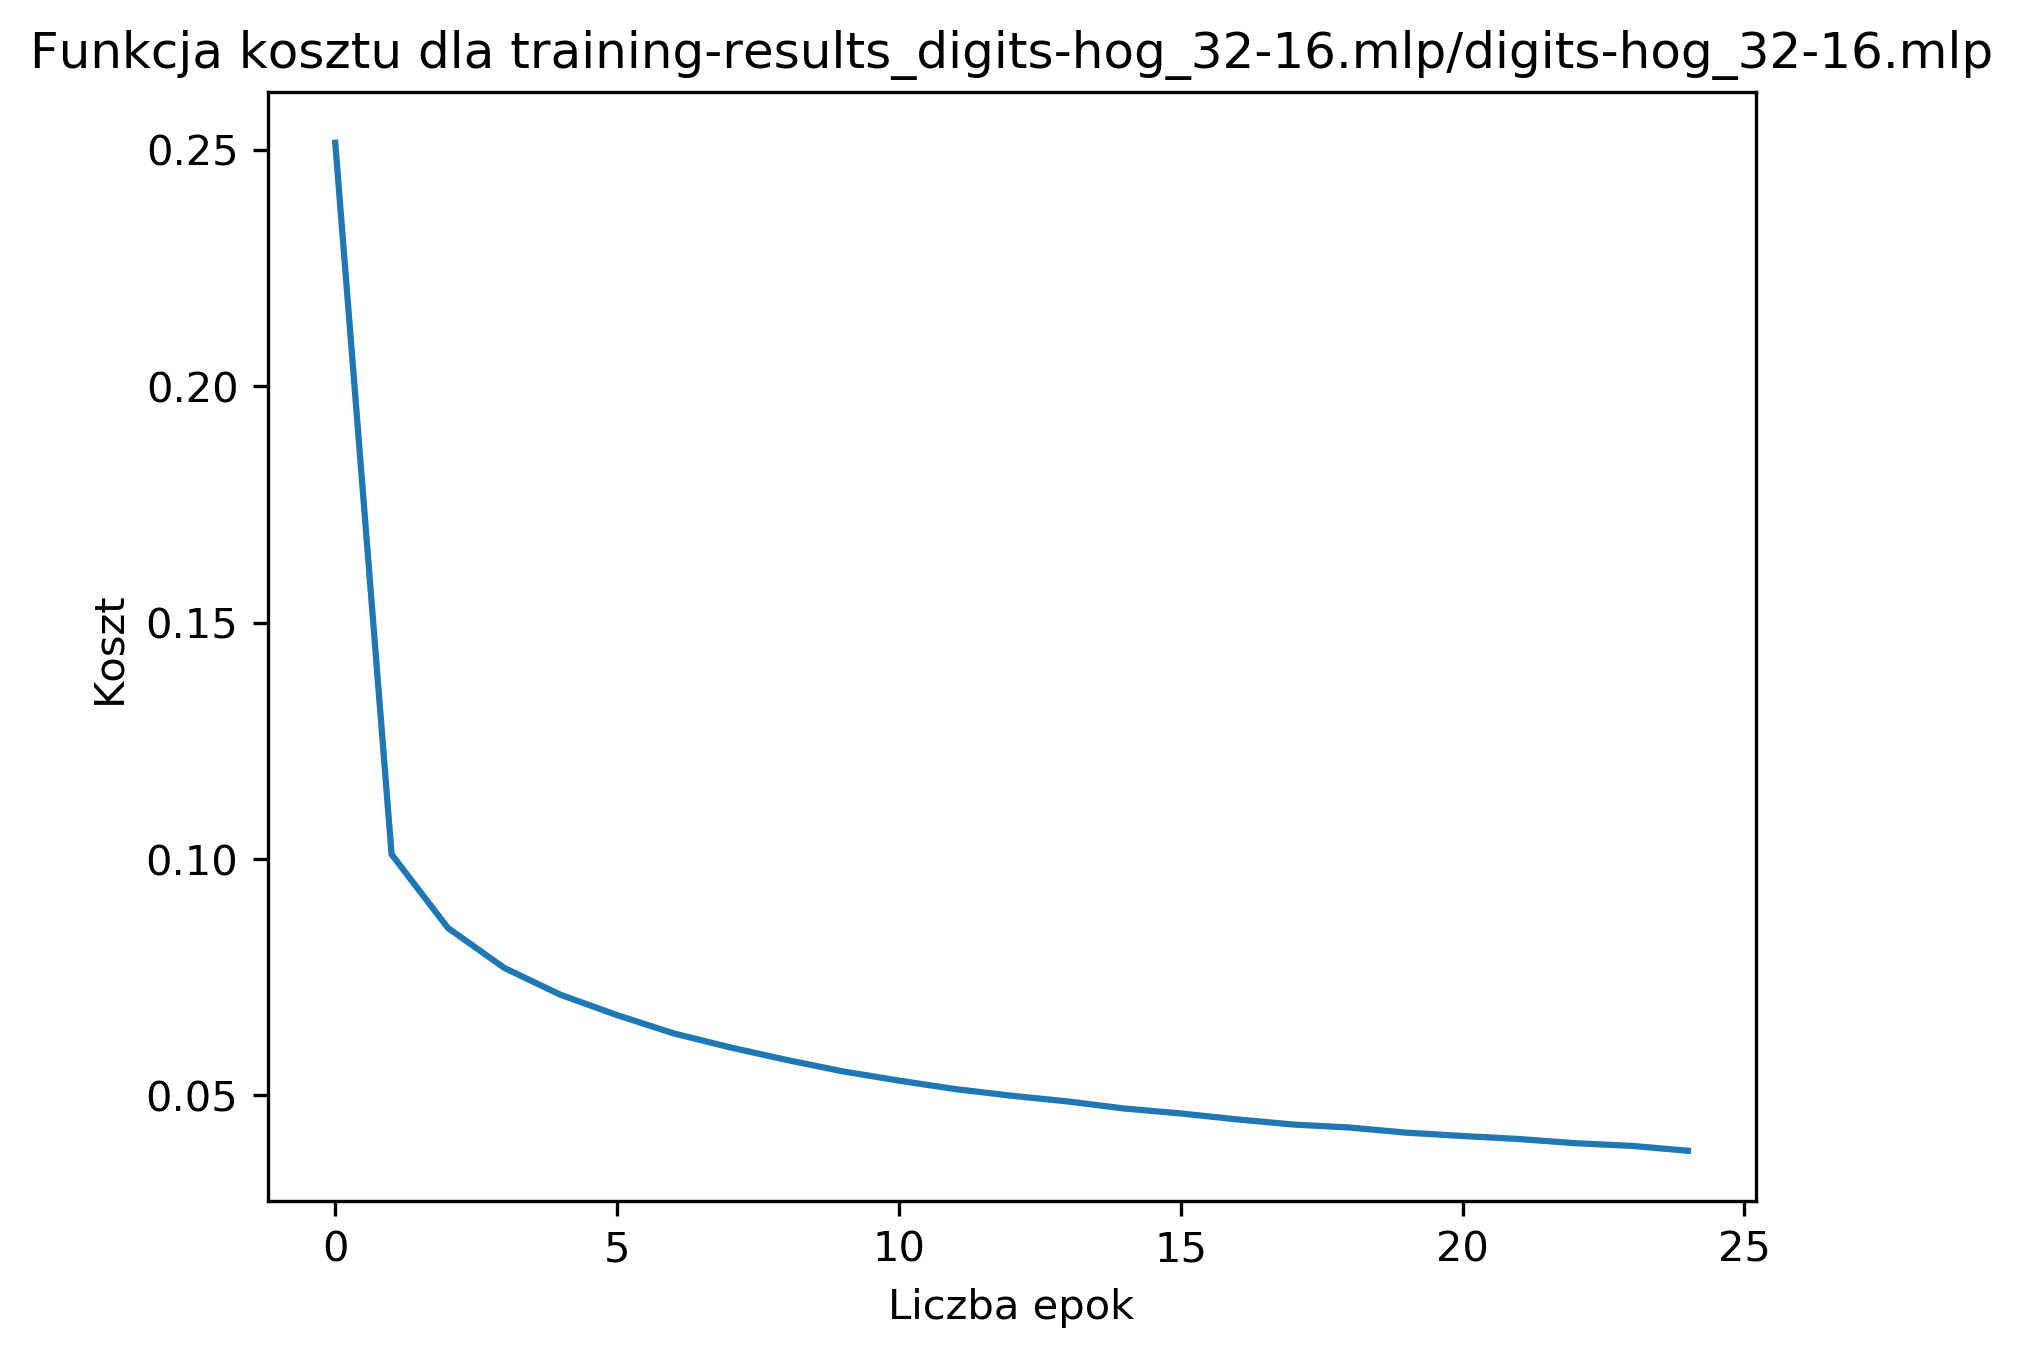
\includegraphics[width=155mm]{wykresy/digits-hog_32-16_mlp_cost.png}
                    \caption{Tryb z standaryzowanymi danymi}
                \end{figure}
                \begin{figure}[!htbp]
                    \centering
                    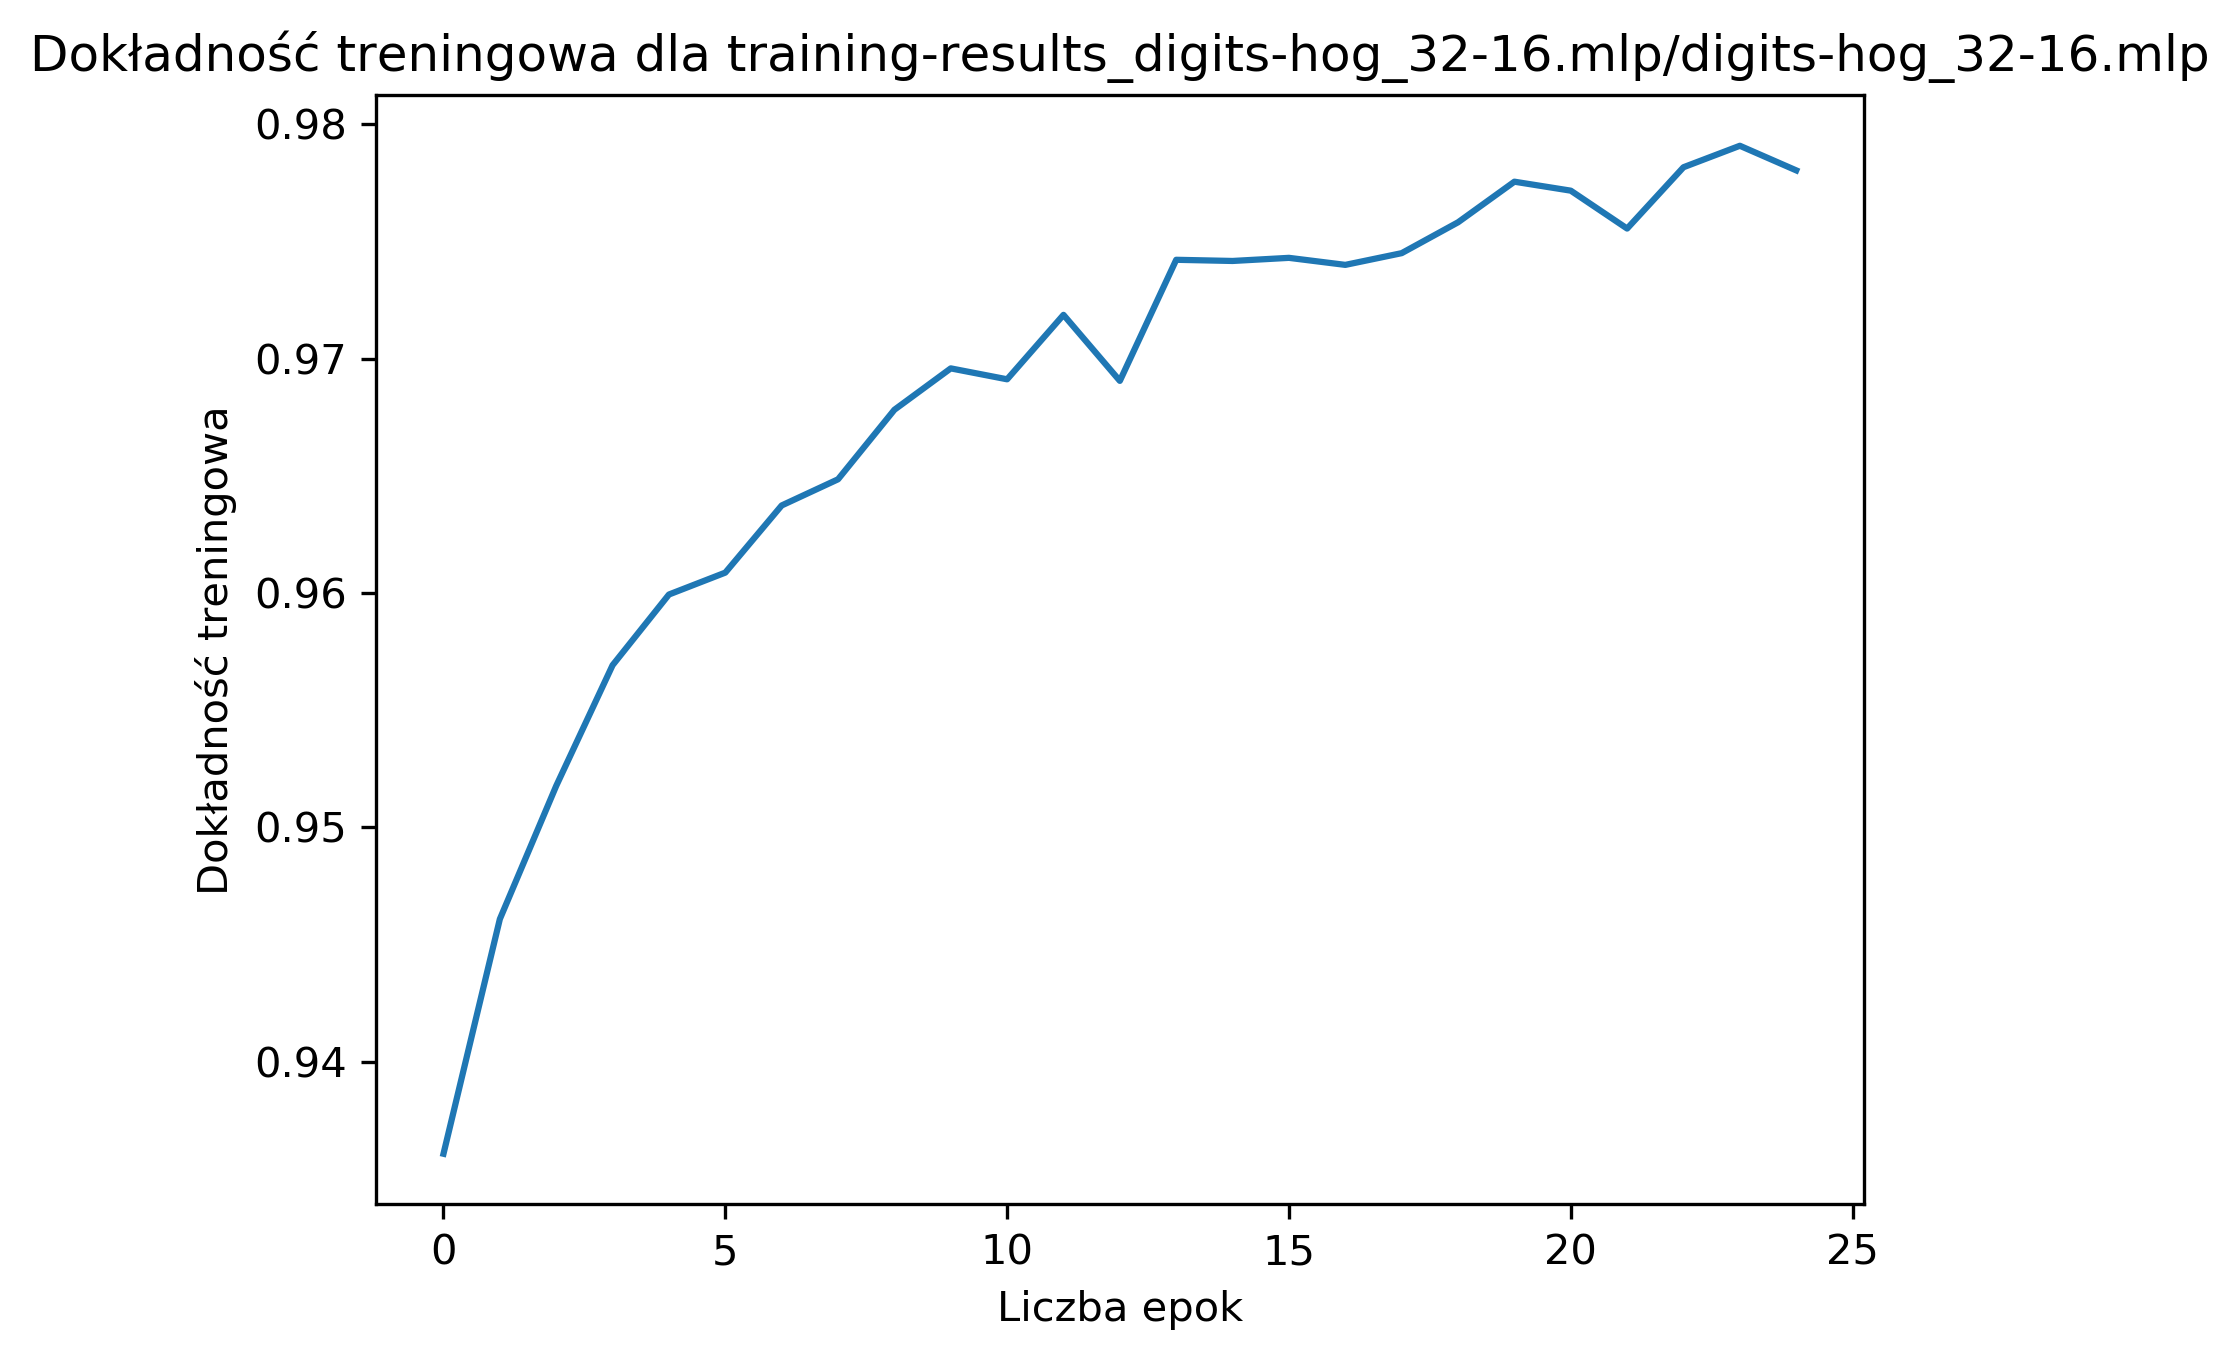
\includegraphics[width=155mm]{wykresy/digits-hog_32-16_mlp_training-accuracy.png}
                    \caption{Tryb z standaryzowanymi danymi}
                \end{figure}
                \begin{figure}[!htbp]
                    \centering
                    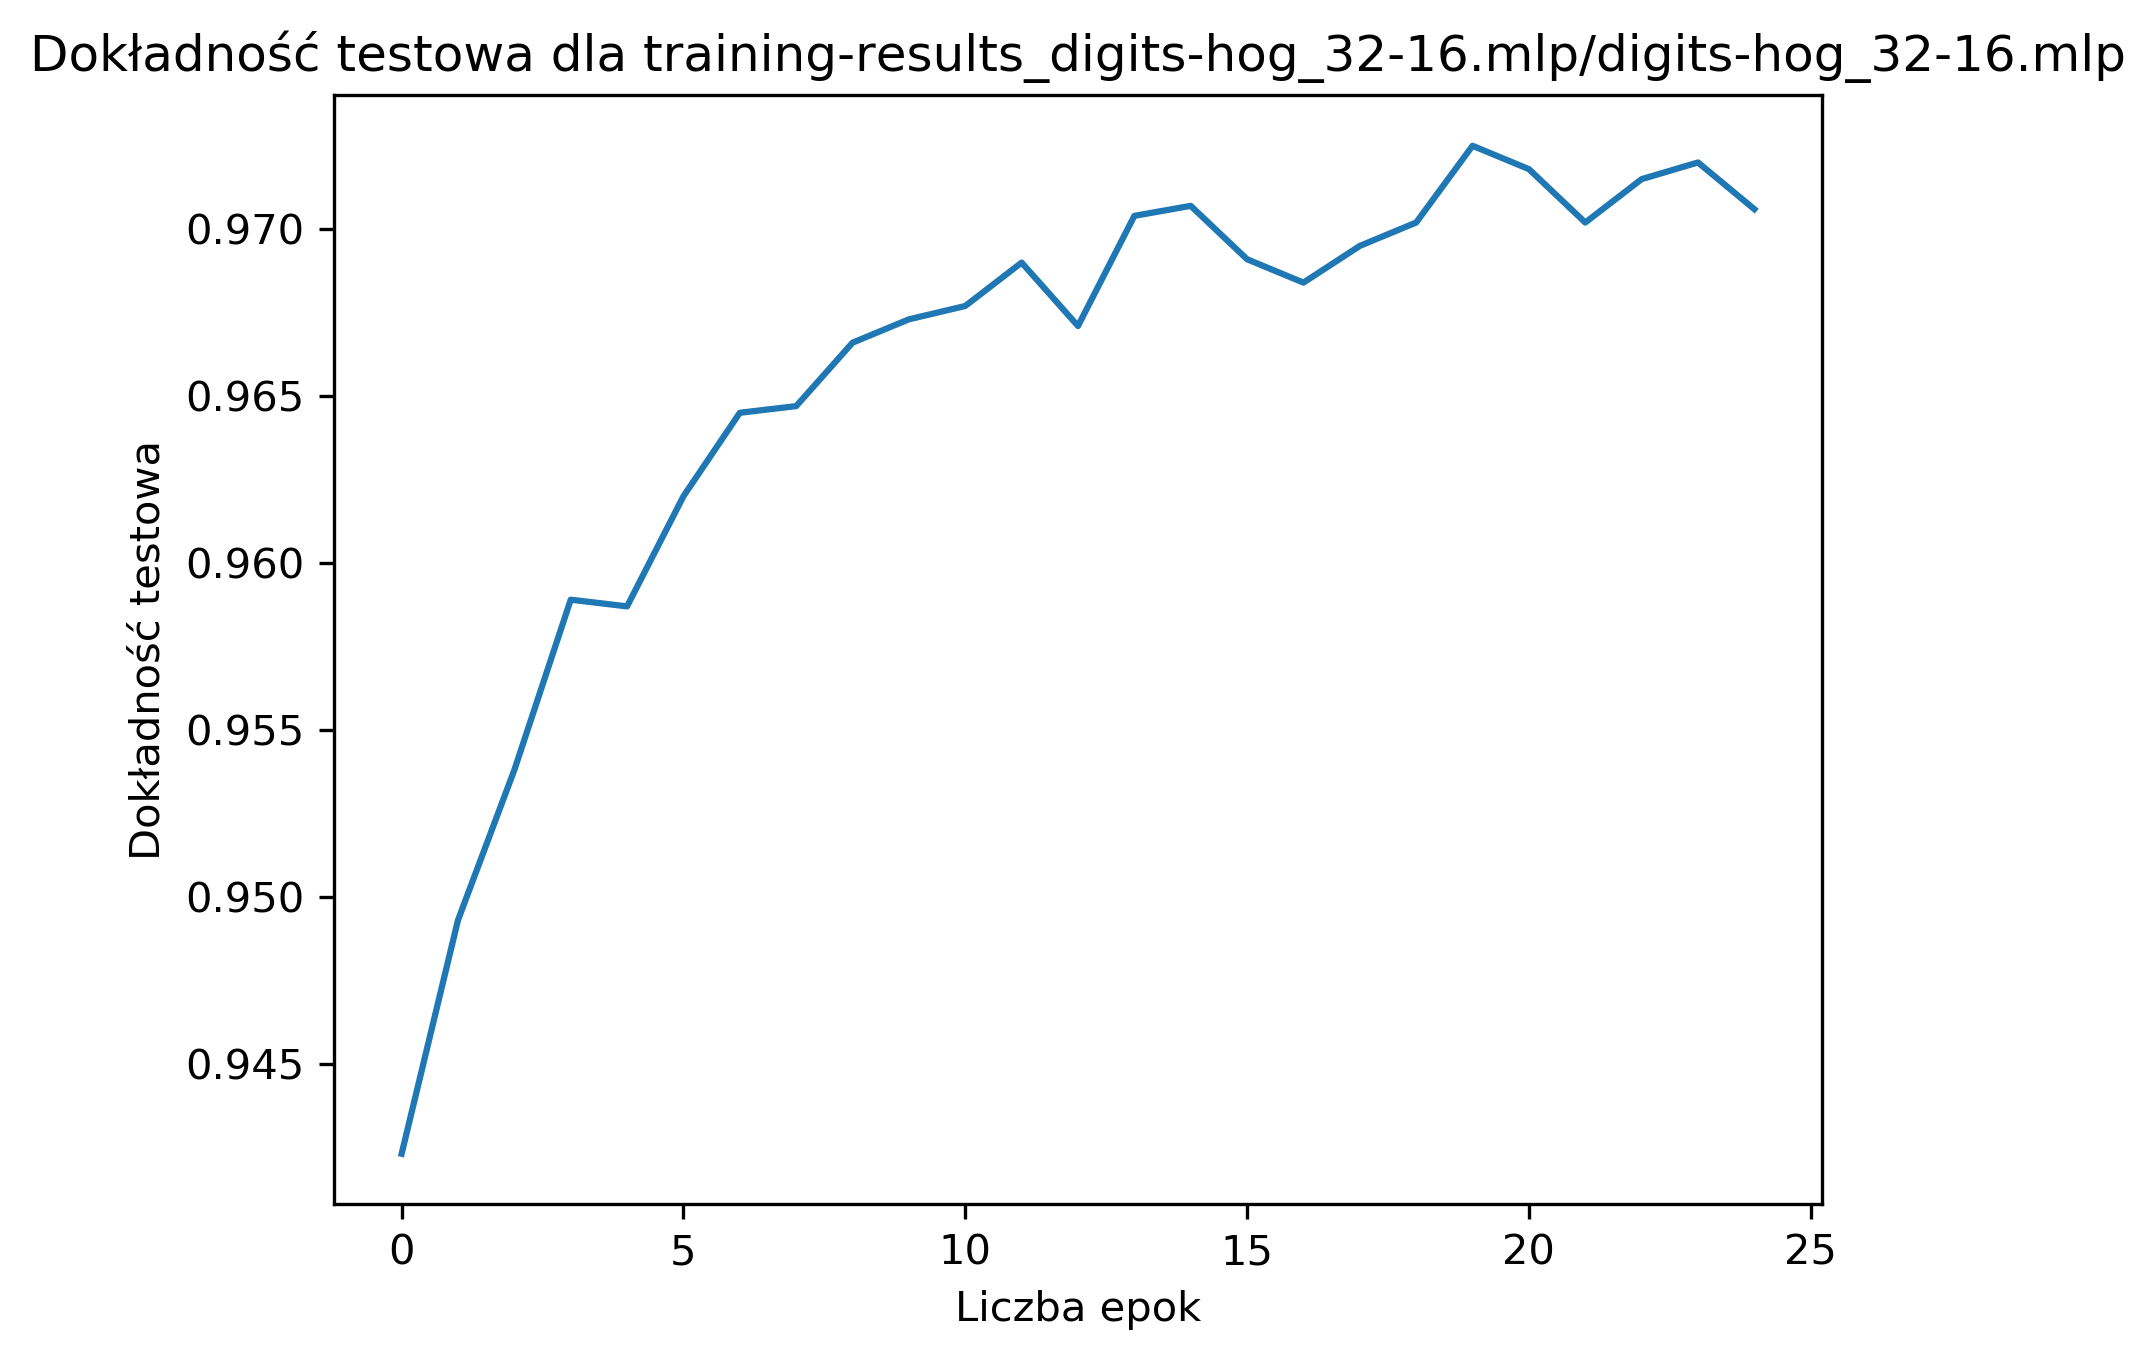
\includegraphics[width=155mm]{wykresy/digits-hog_32-16_mlp_testing-accuracy.png}
                    \caption{Tryb z standaryzowanymi danymi}
                \end{figure}
                \FloatBarrier
            %---------------------------------------------------%
                \textbf{Histogram gradientu 128}
                \begin{figure}[!htbp]
                    \centering
                    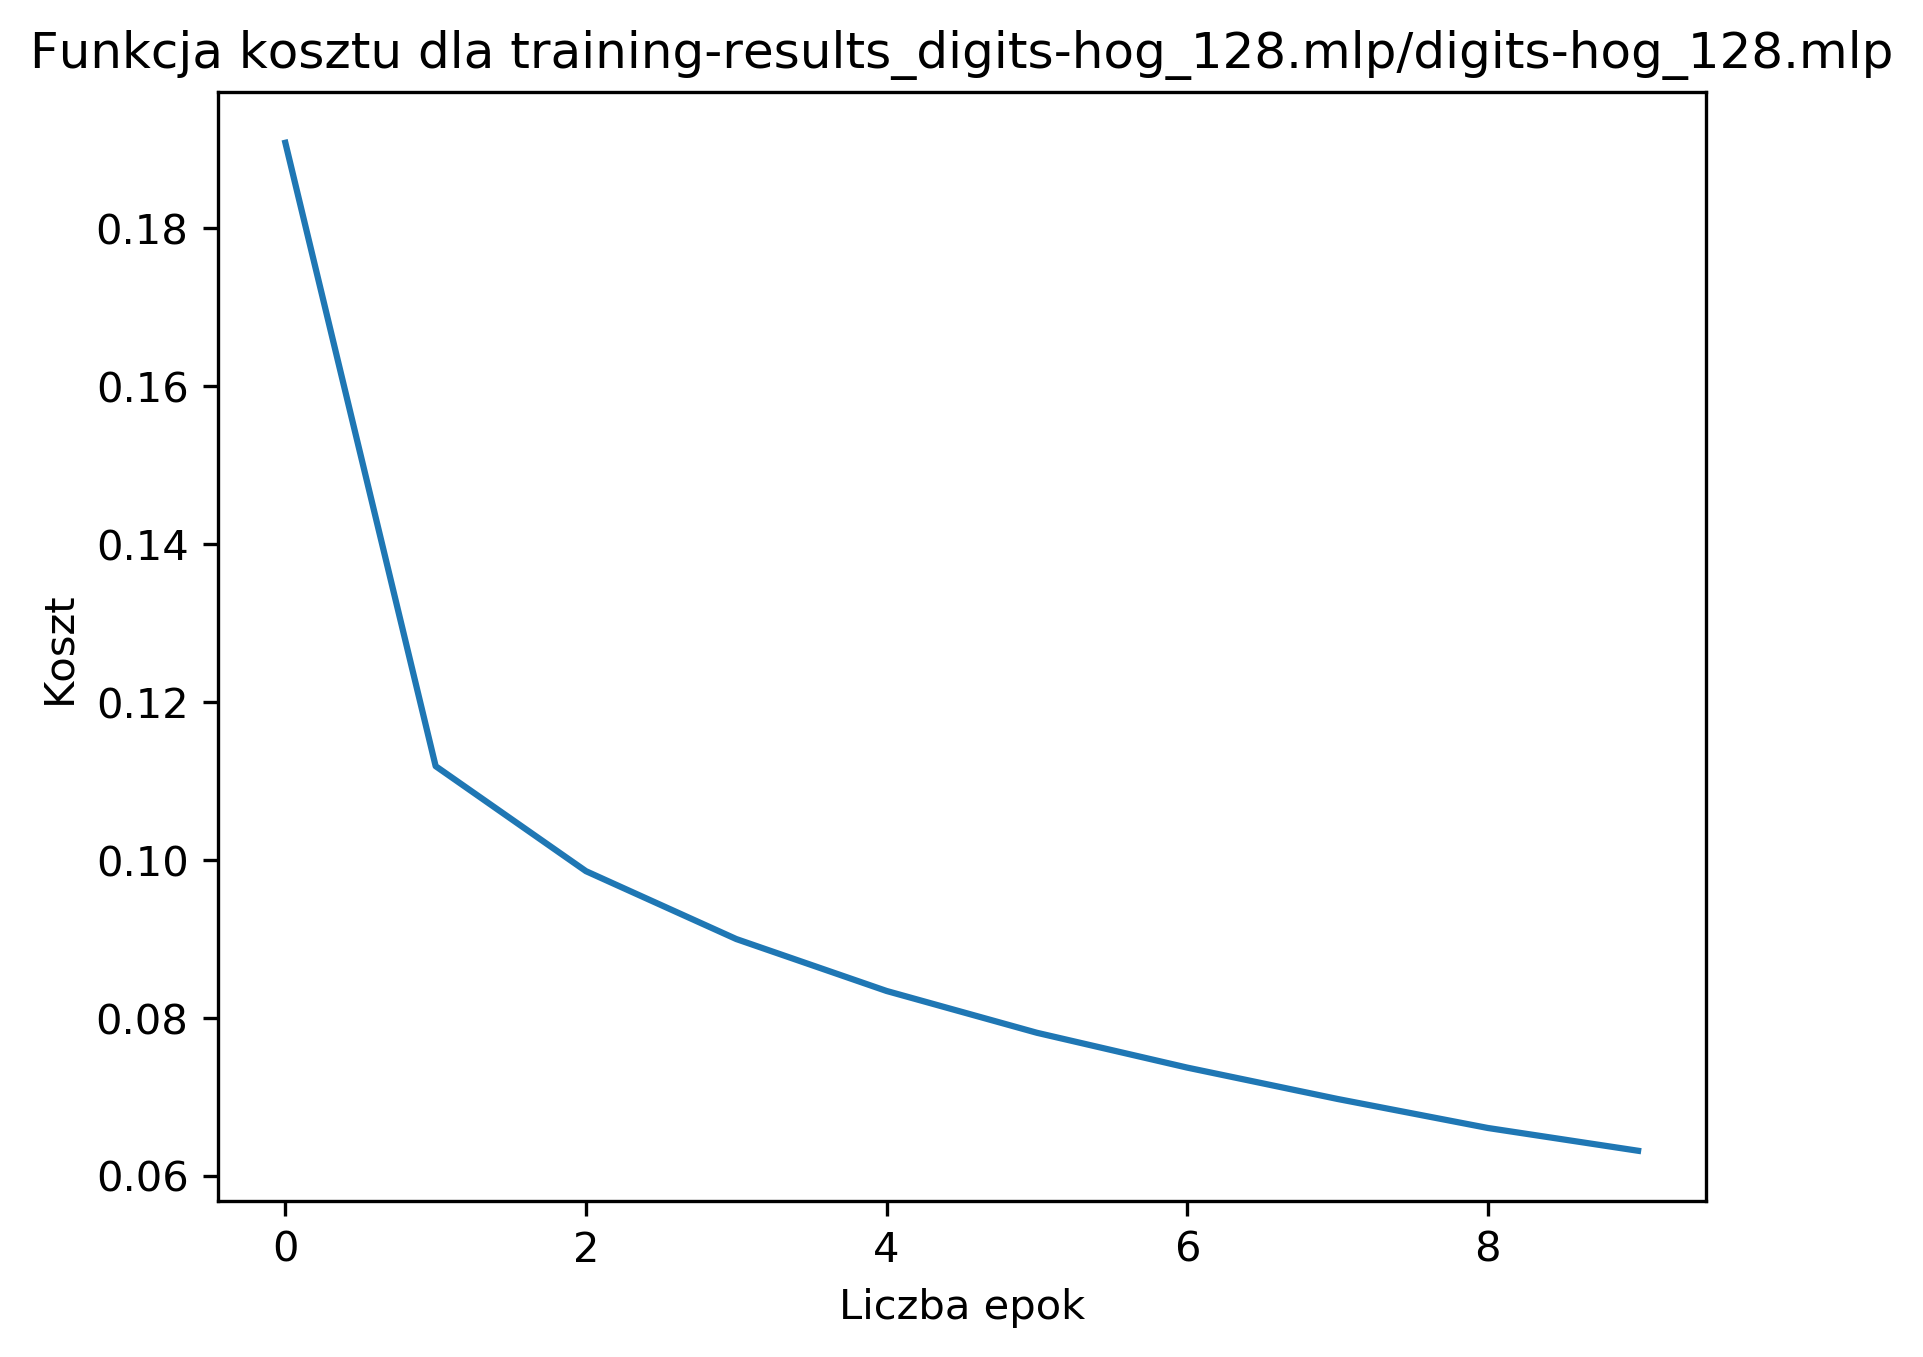
\includegraphics[width=145mm]{wykresy/digits-hog_128_mlp_cost.png}
                    \caption{Tryb z standaryzowanymi danymi}
                \end{figure}
                \begin{figure}[!htbp]
                    \centering
                    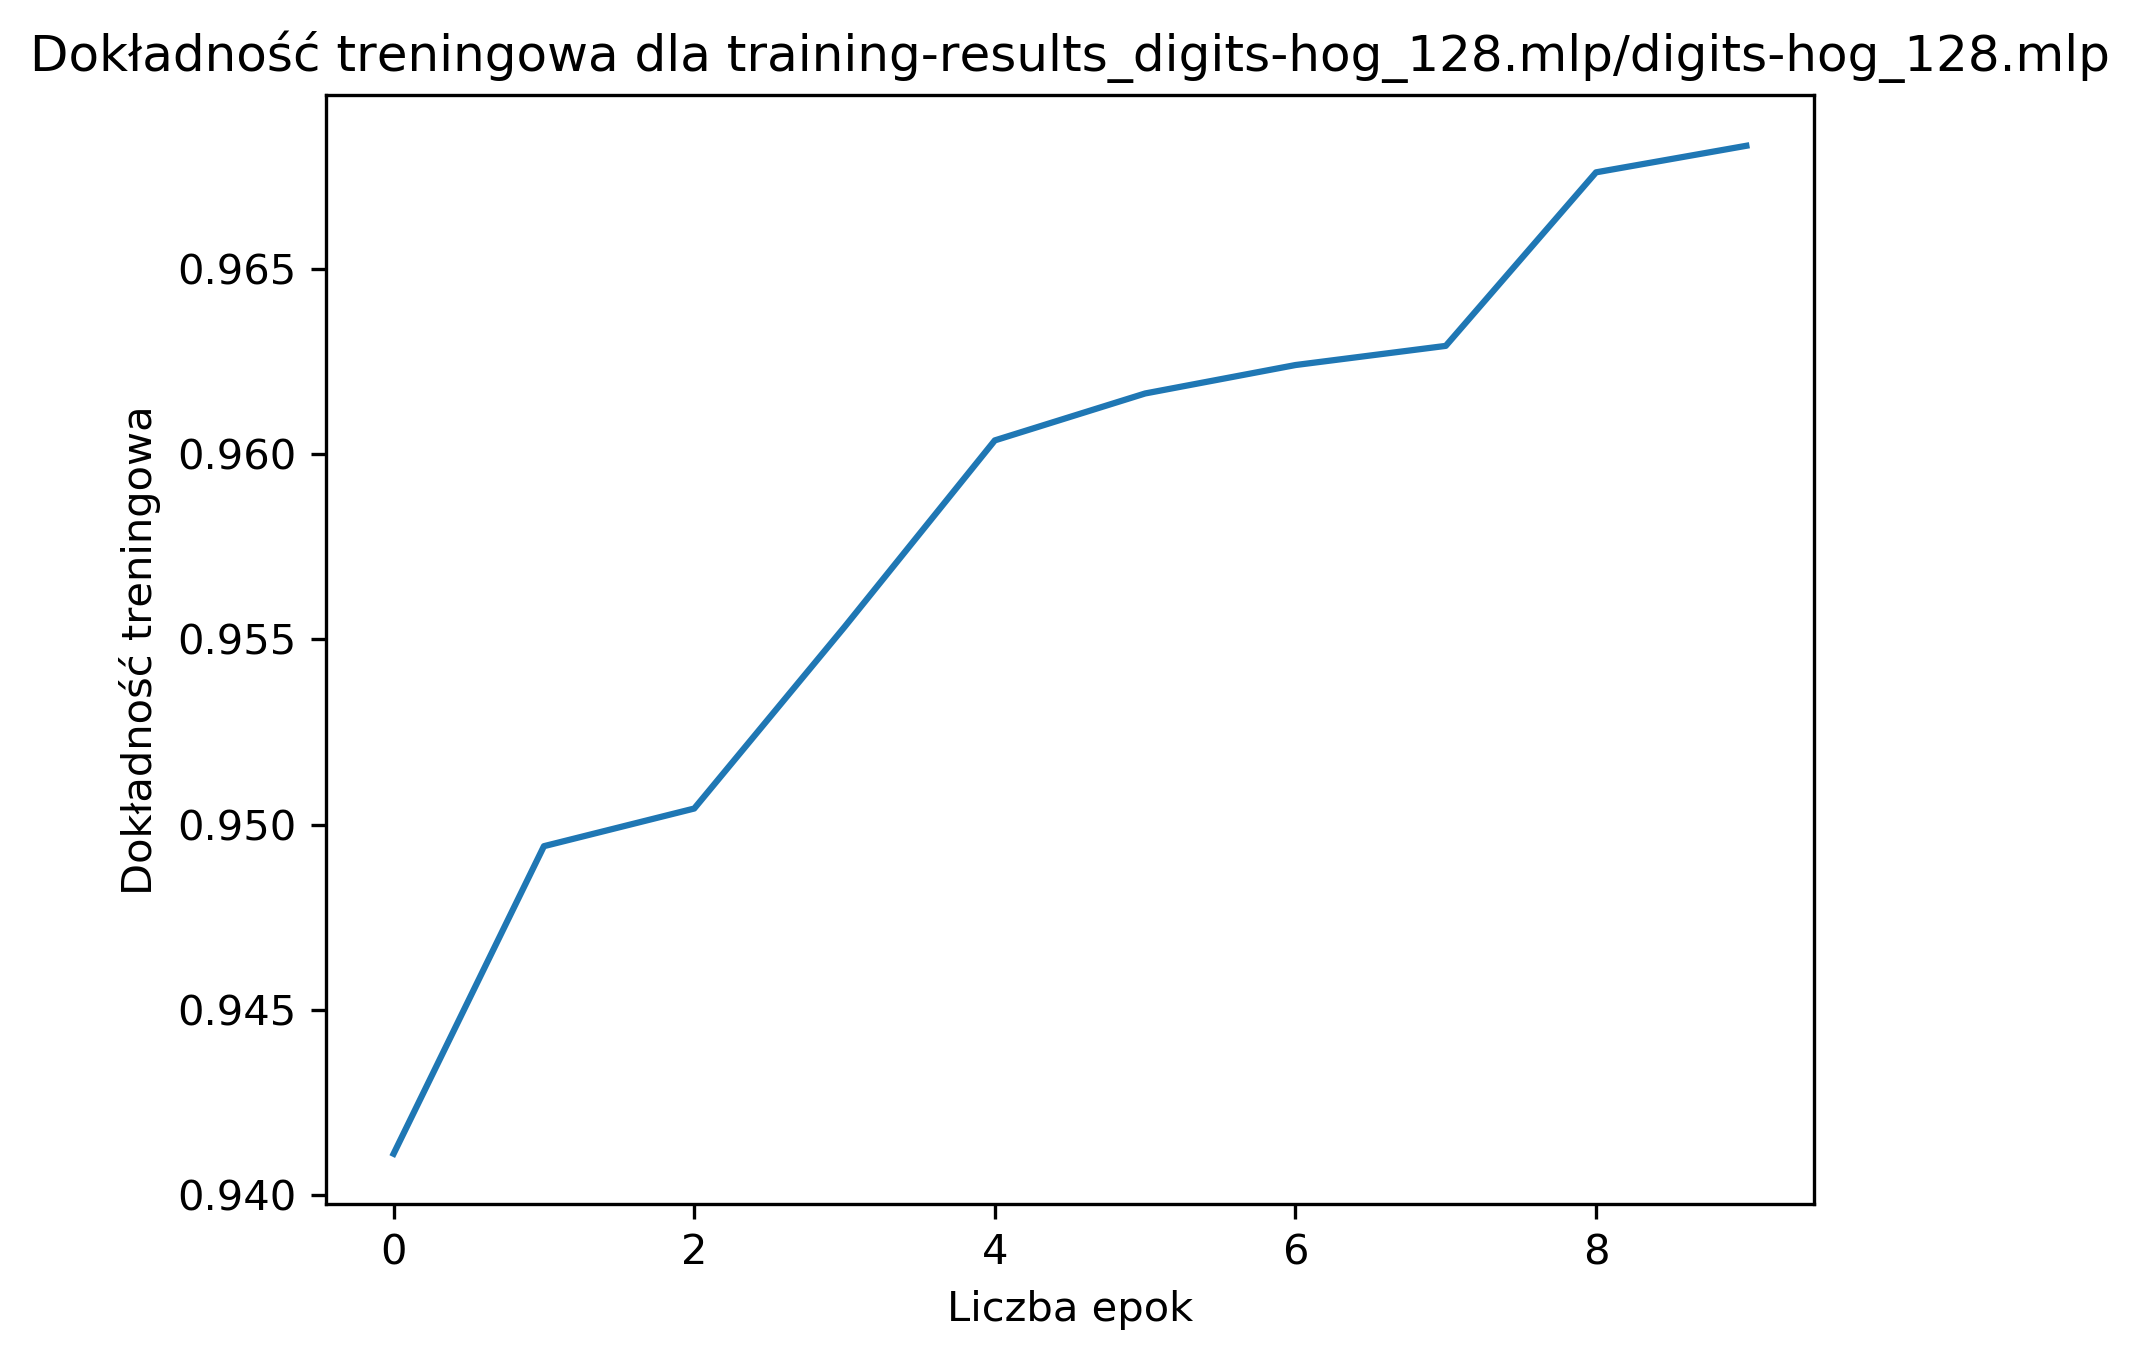
\includegraphics[width=145mm]{wykresy/digits-hog_128_mlp_training-accuracy.png}
                    \caption{Tryb z standaryzowanymi danymi}
                \end{figure}
                \begin{figure}[!htbp]
                    \centering
                    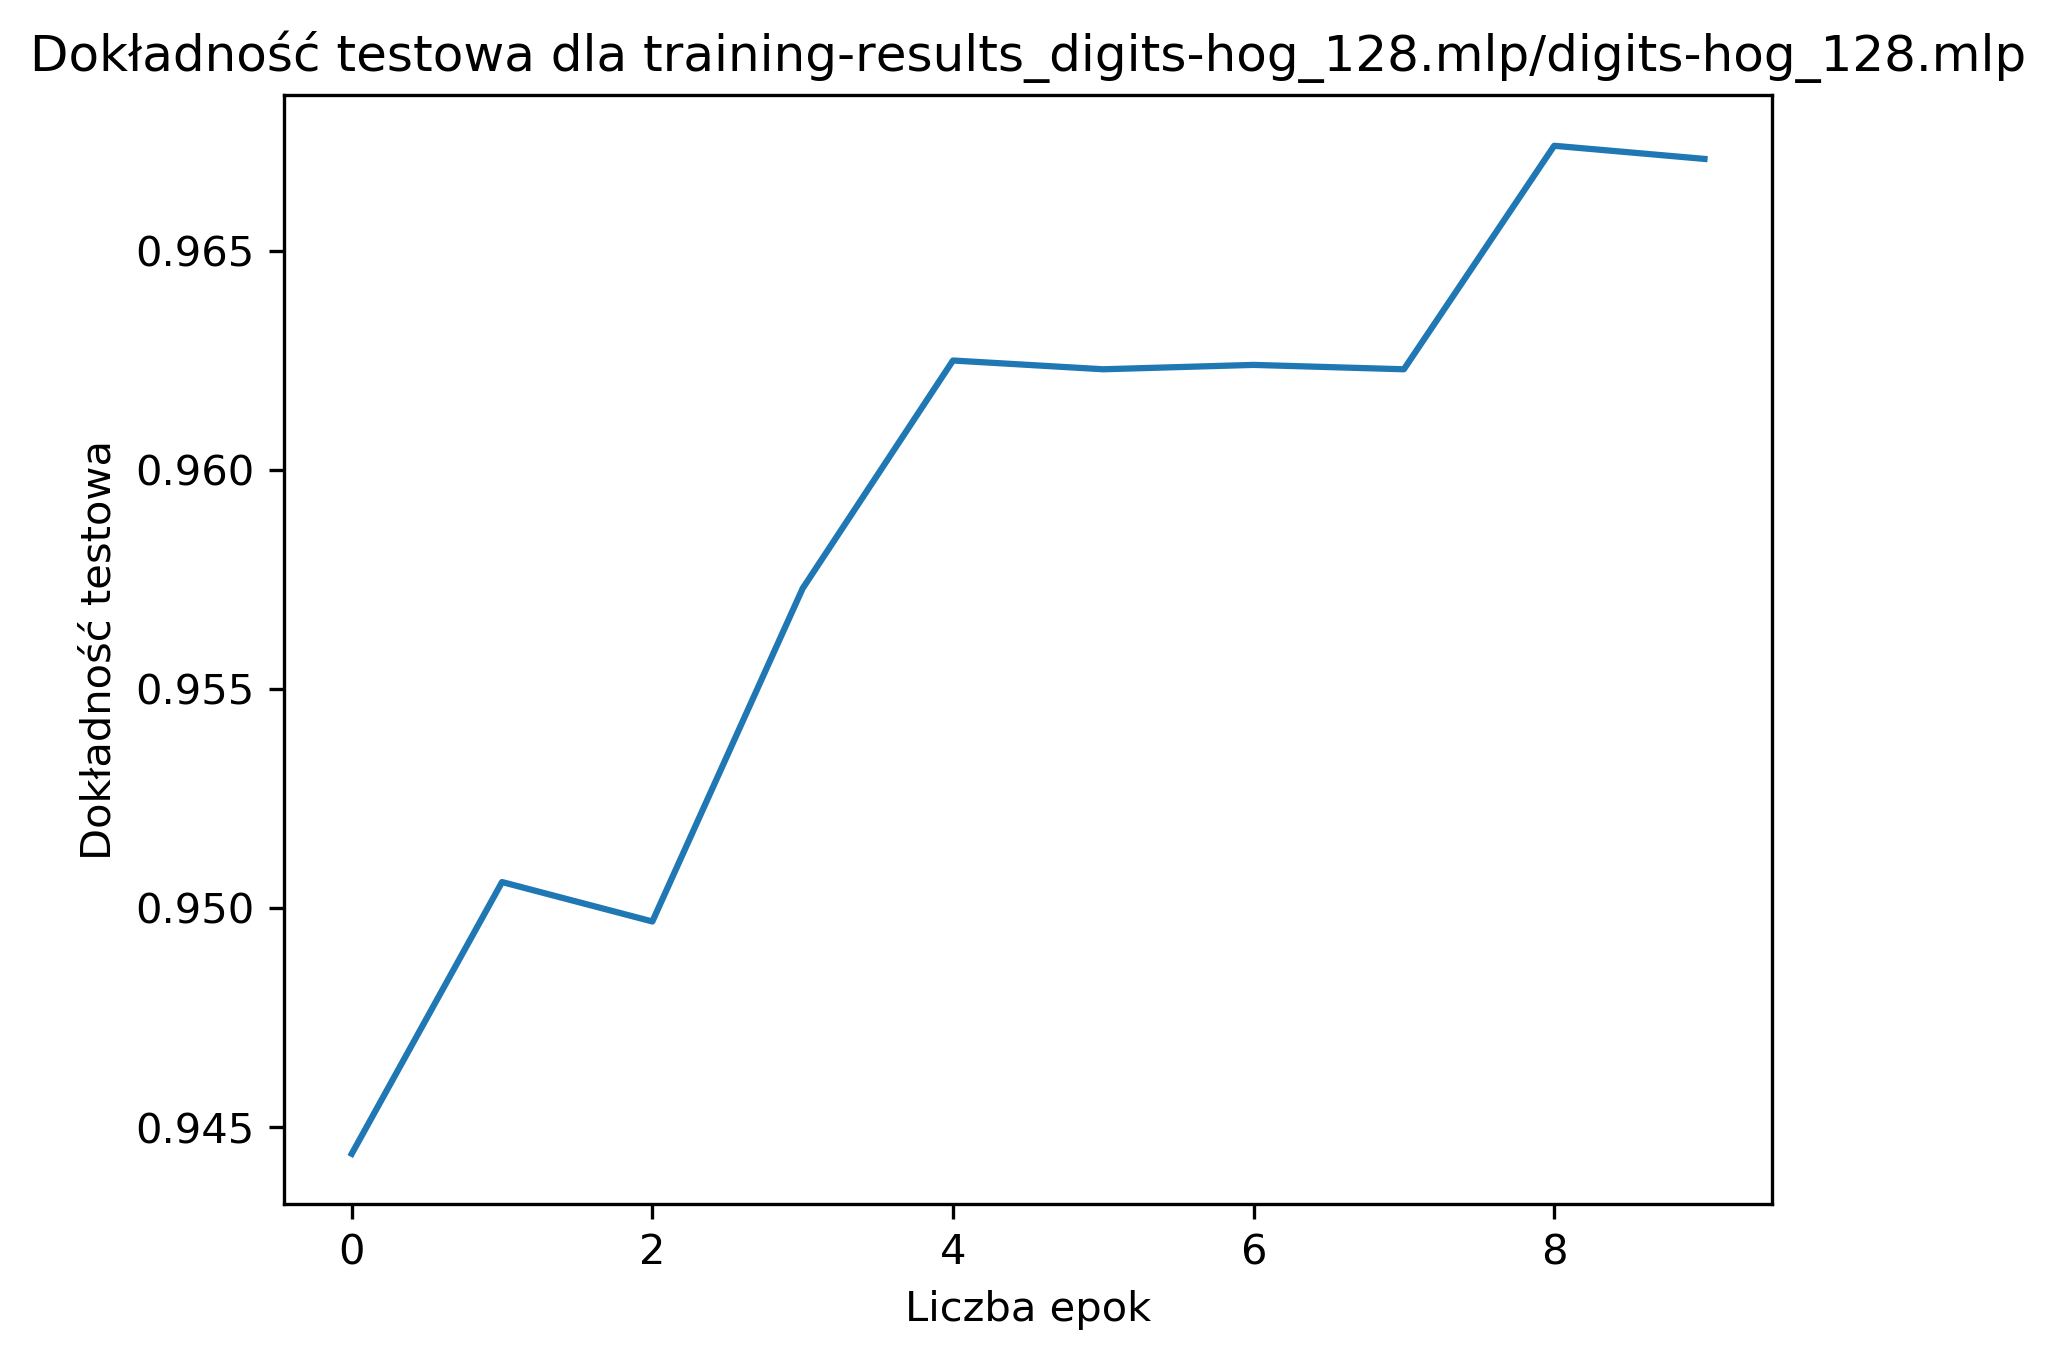
\includegraphics[width=145mm]{wykresy/digits-hog_128_mlp_testing-accuracy.png}
                    \caption{Tryb z standaryzowanymi danymi}
                \end{figure}
                \FloatBarrier
            %---------------------------------------------------%
                \textbf{Dane normalizowane 8}
                \begin{figure}[!htbp]
                    \centering
                    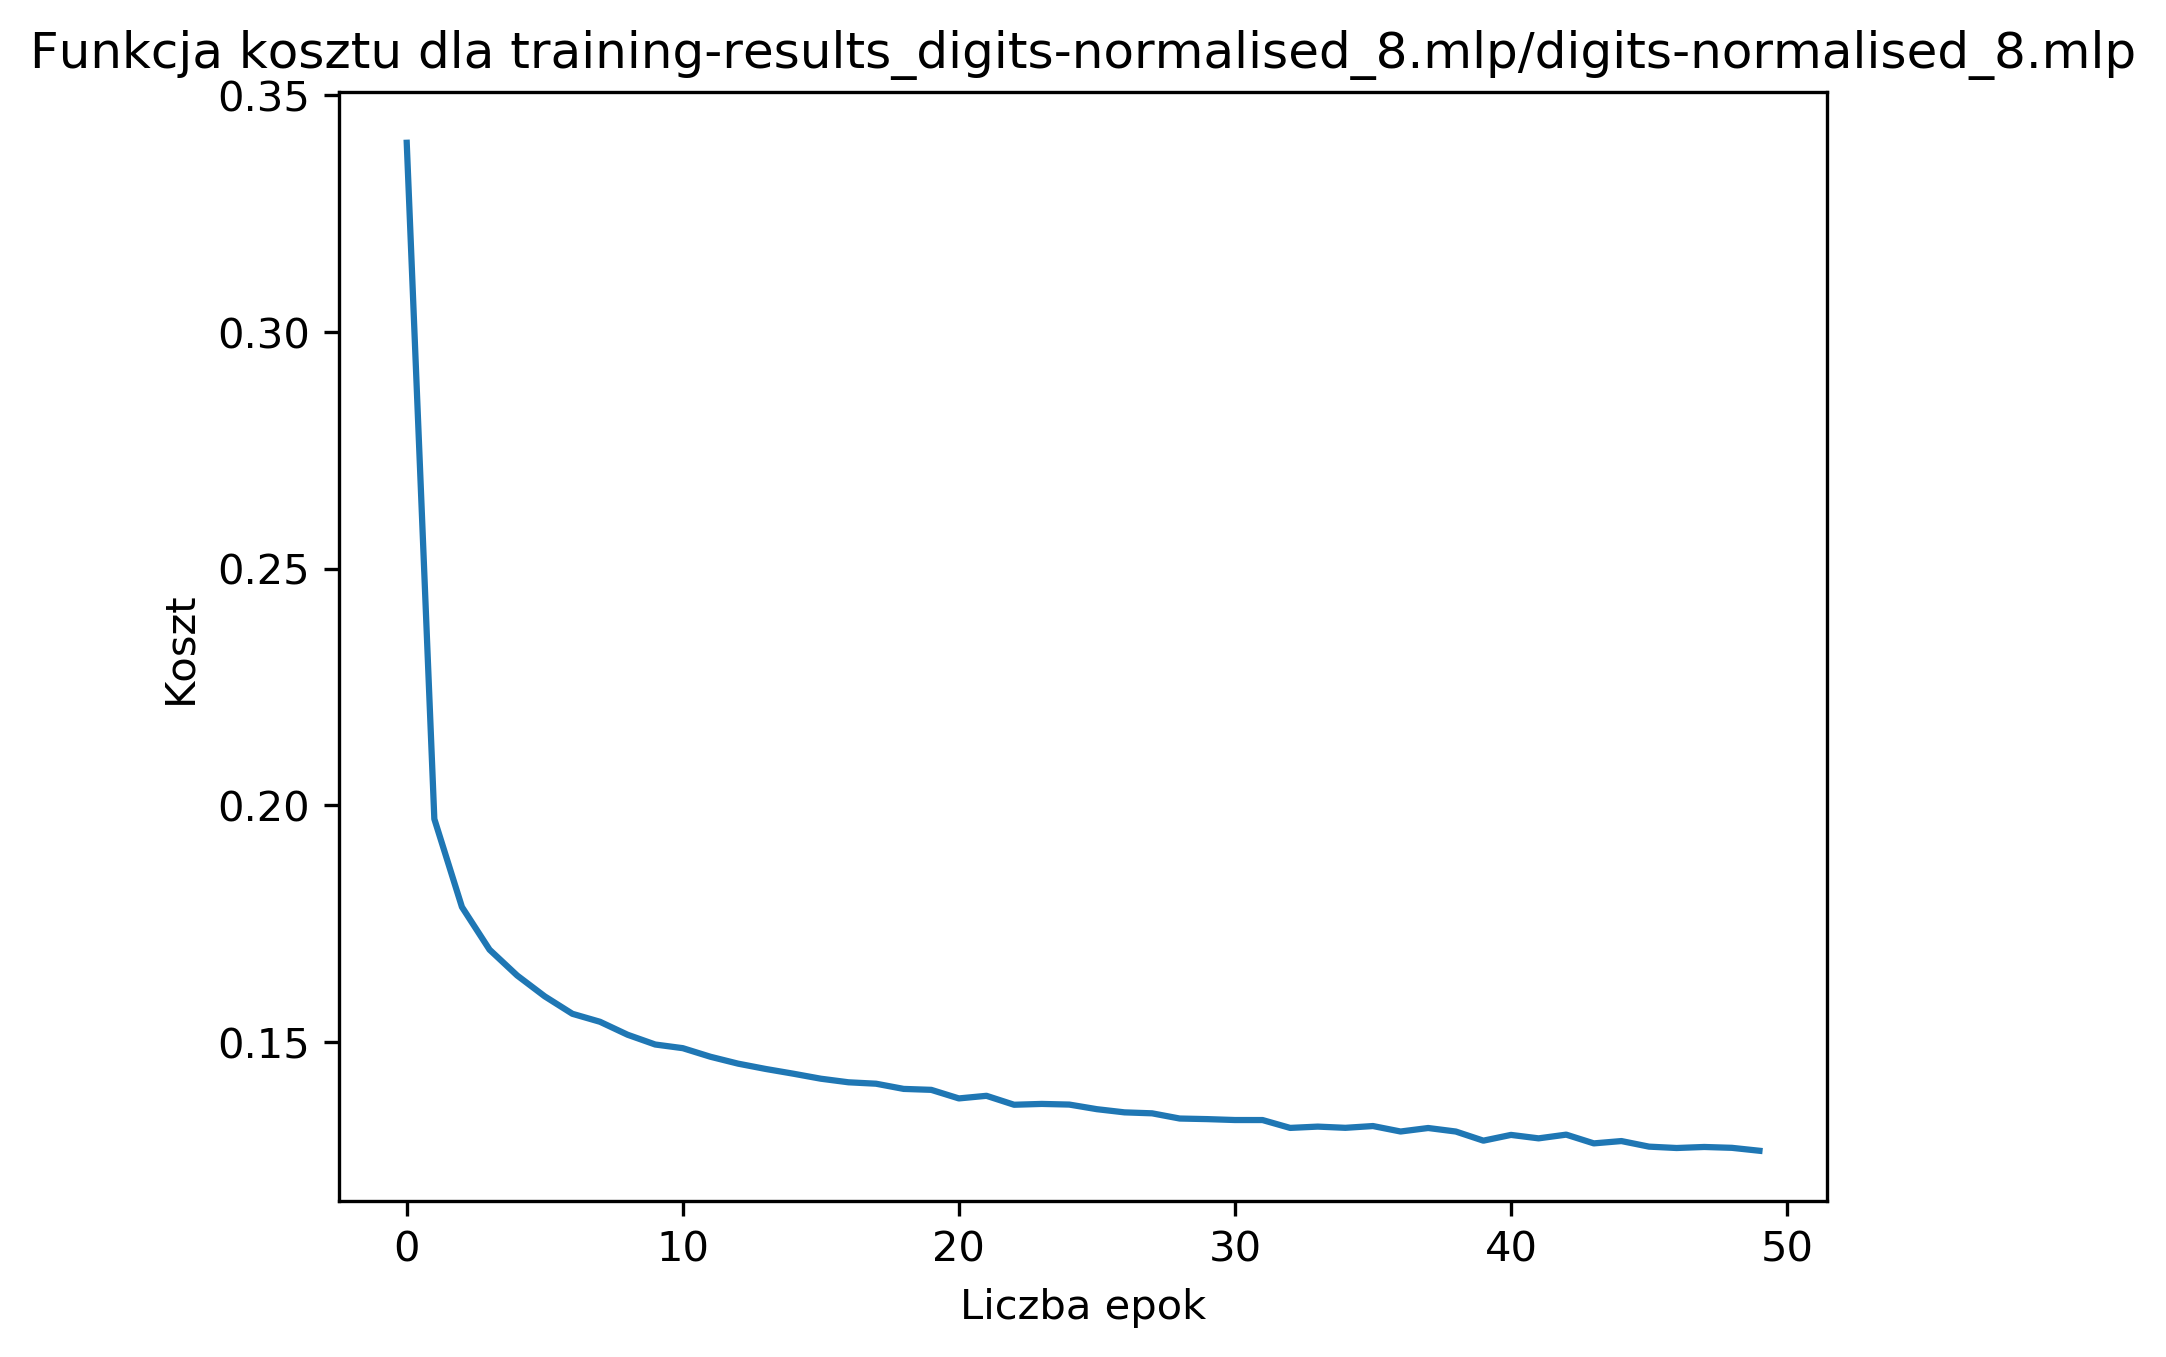
\includegraphics[width=145mm]{wykresy/digits-normalised_8_mlp_cost.png}
                    \caption{Tryb z normalizowanymi danymi}
                \end{figure}
                \begin{figure}[!htbp]
                    \centering
                    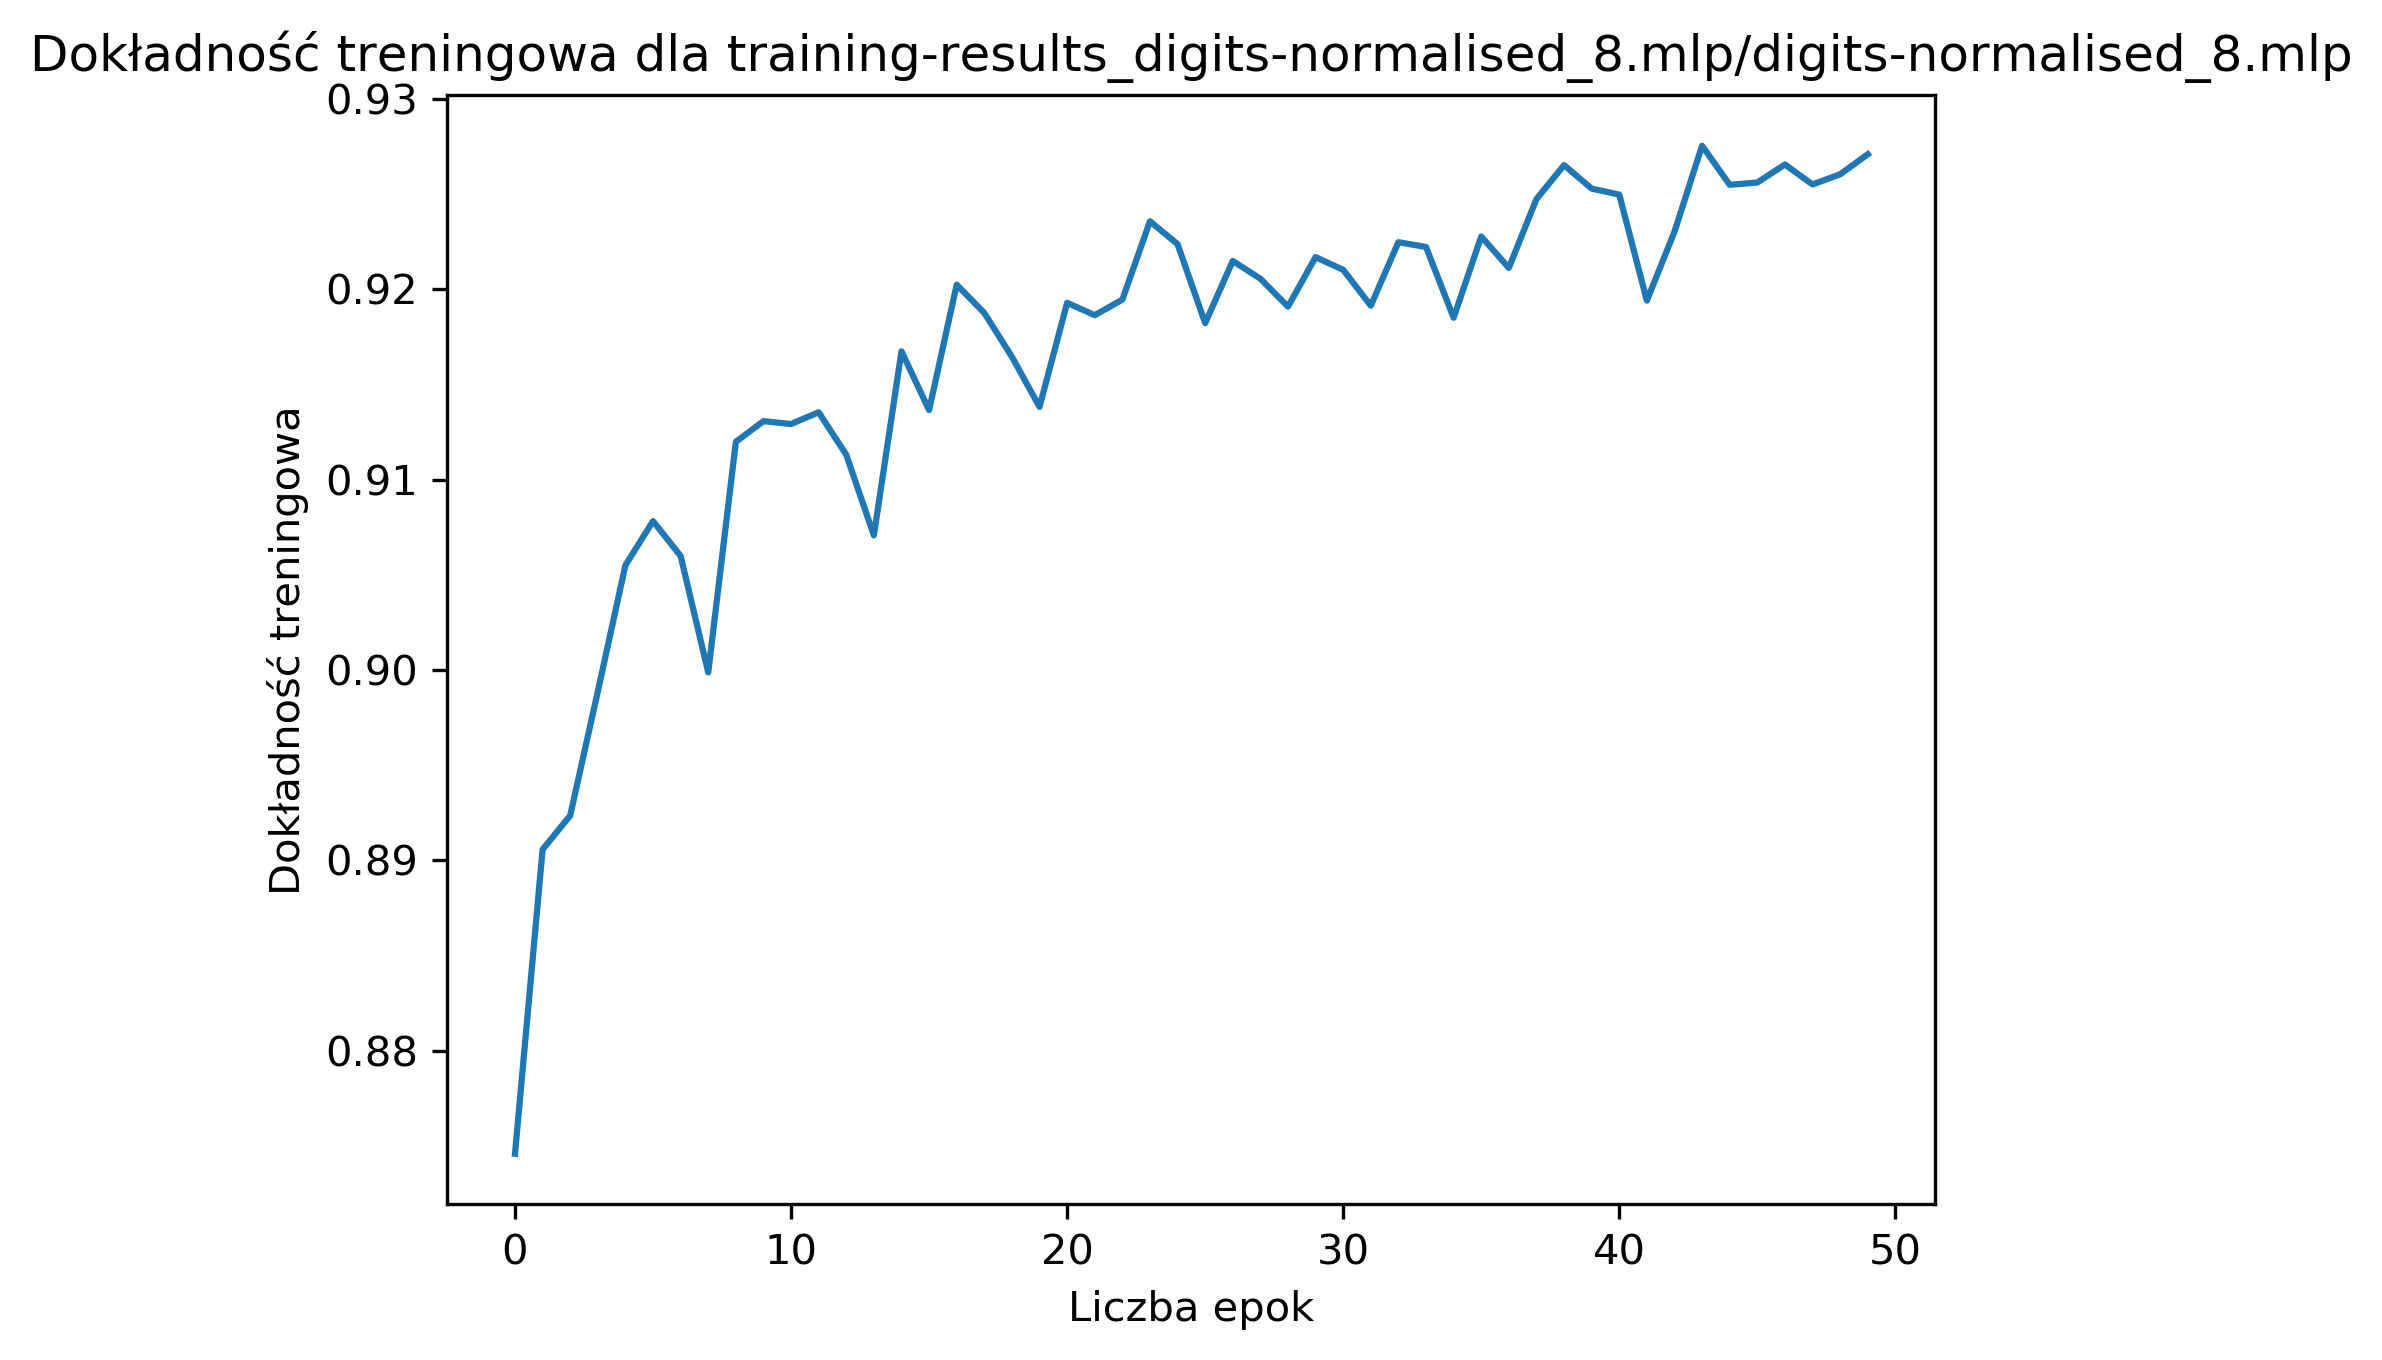
\includegraphics[width=155mm]{wykresy/digits-normalised_8_mlp_training-accuracy.png}
                    \caption{Tryb z normalizowanymi danymi}
                \end{figure}
                \begin{figure}[!htbp]
                    \centering
                    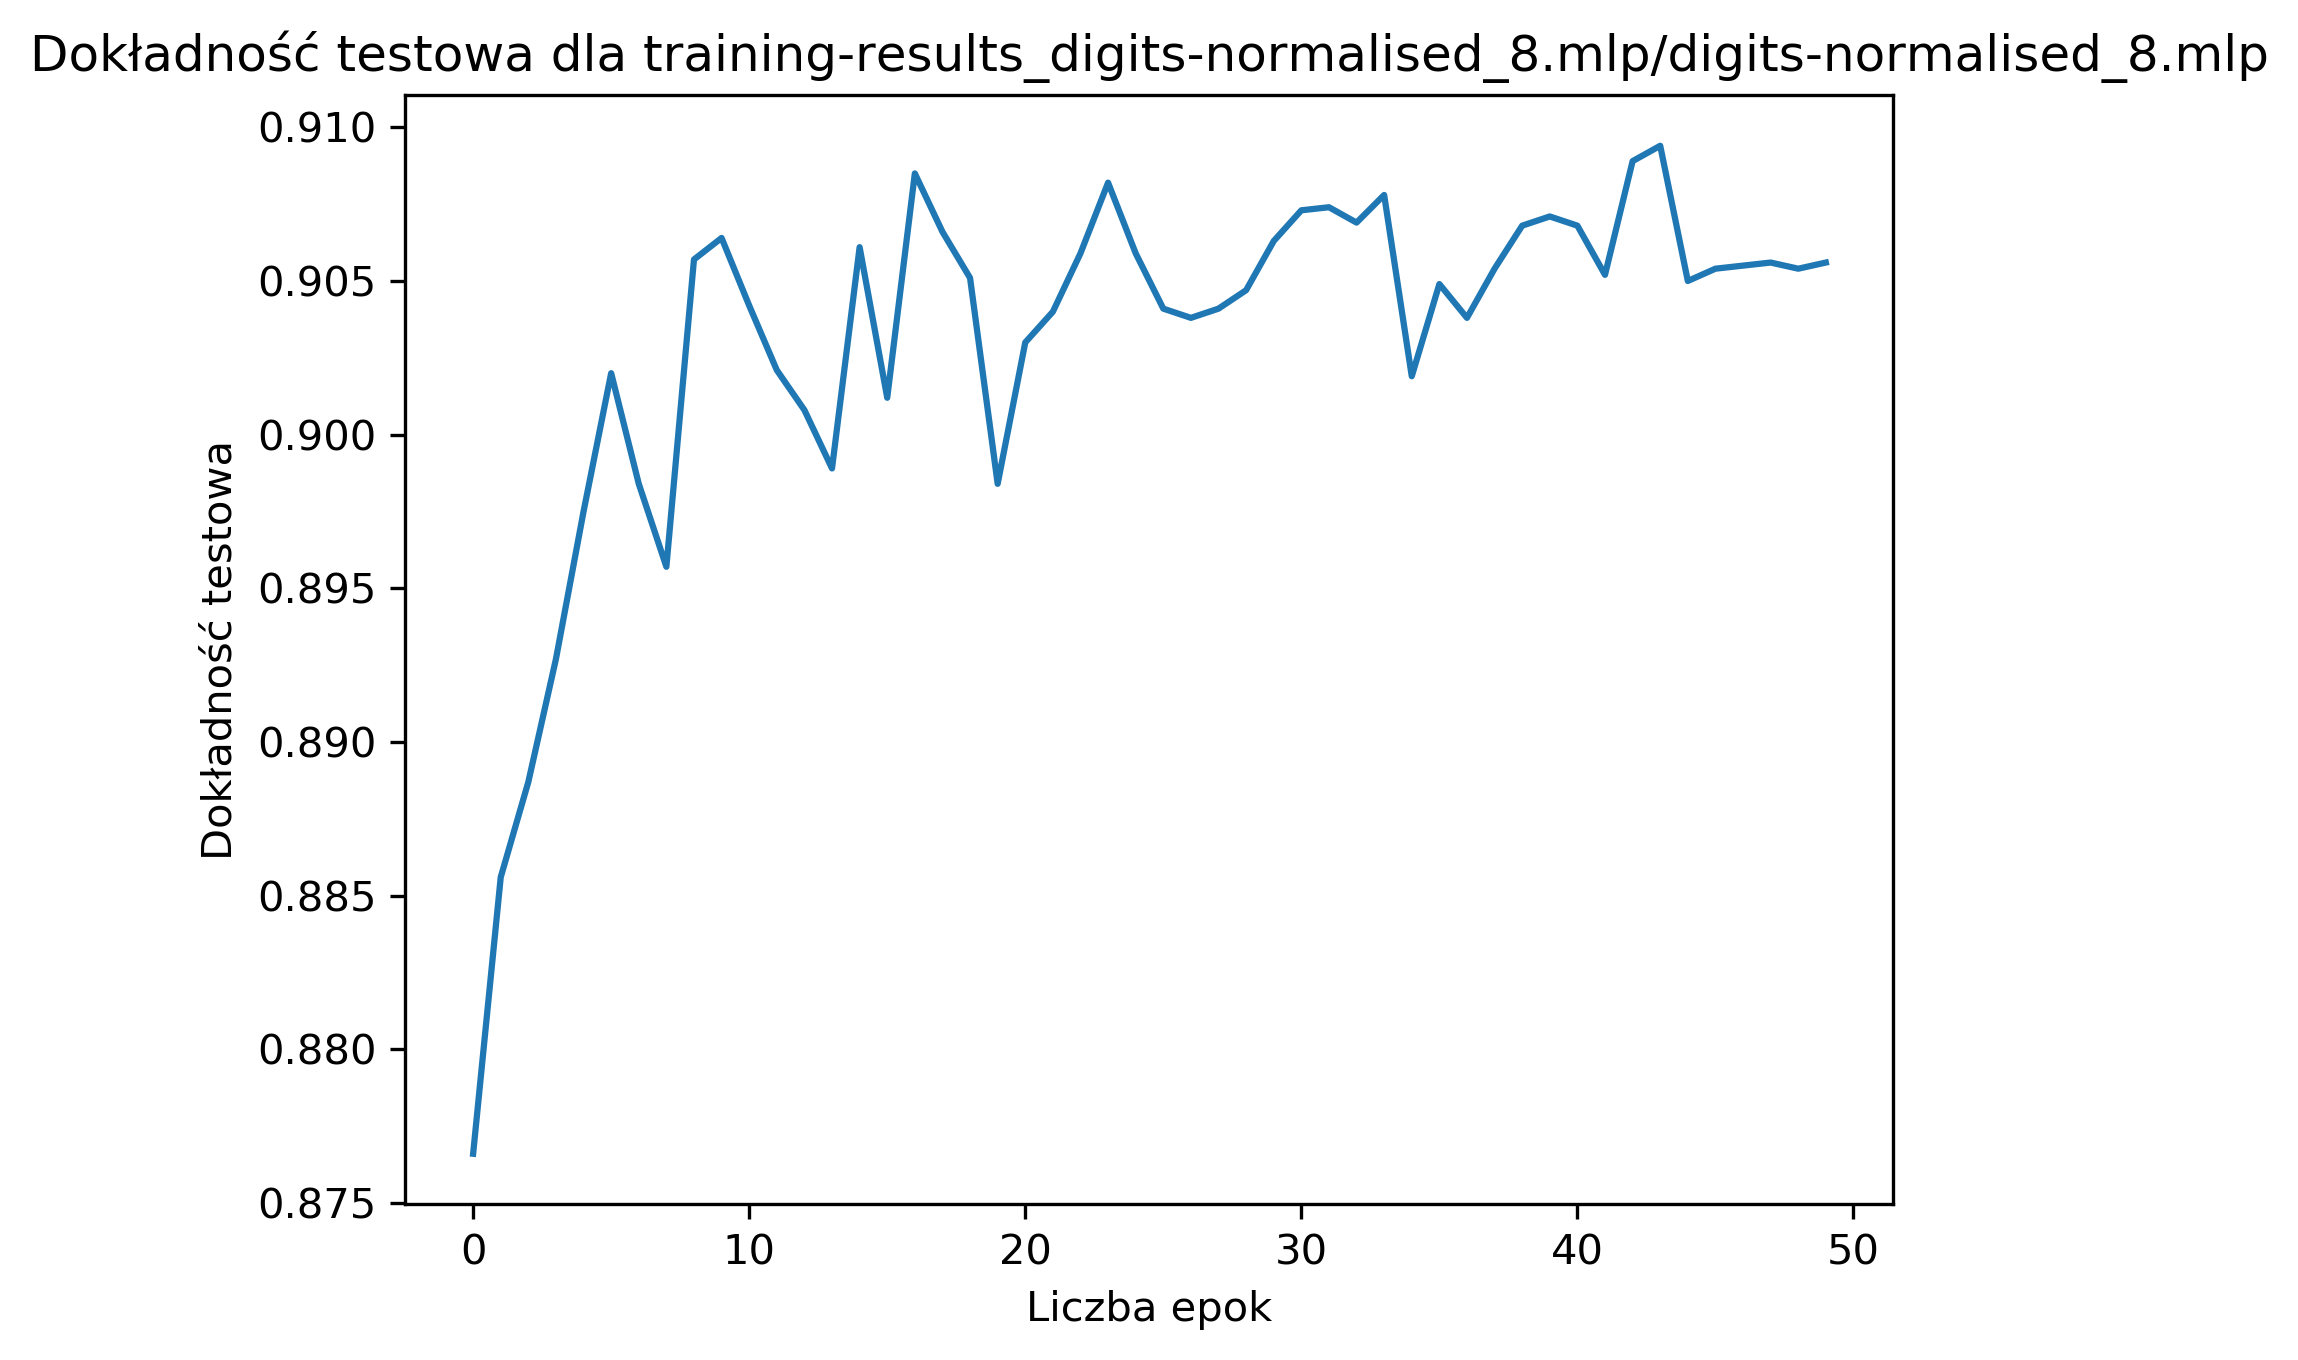
\includegraphics[width=155mm]{wykresy/digits-normalised_8_mlp_testing-accuracy.png}
                    \caption{Tryb z normalizowanymi danymi}
                \end{figure}
                \FloatBarrier
            %---------------------------------------------------%
                \textbf{Dane normalizowane 32-16}
                \begin{figure}[!htbp]
                    \centering
                    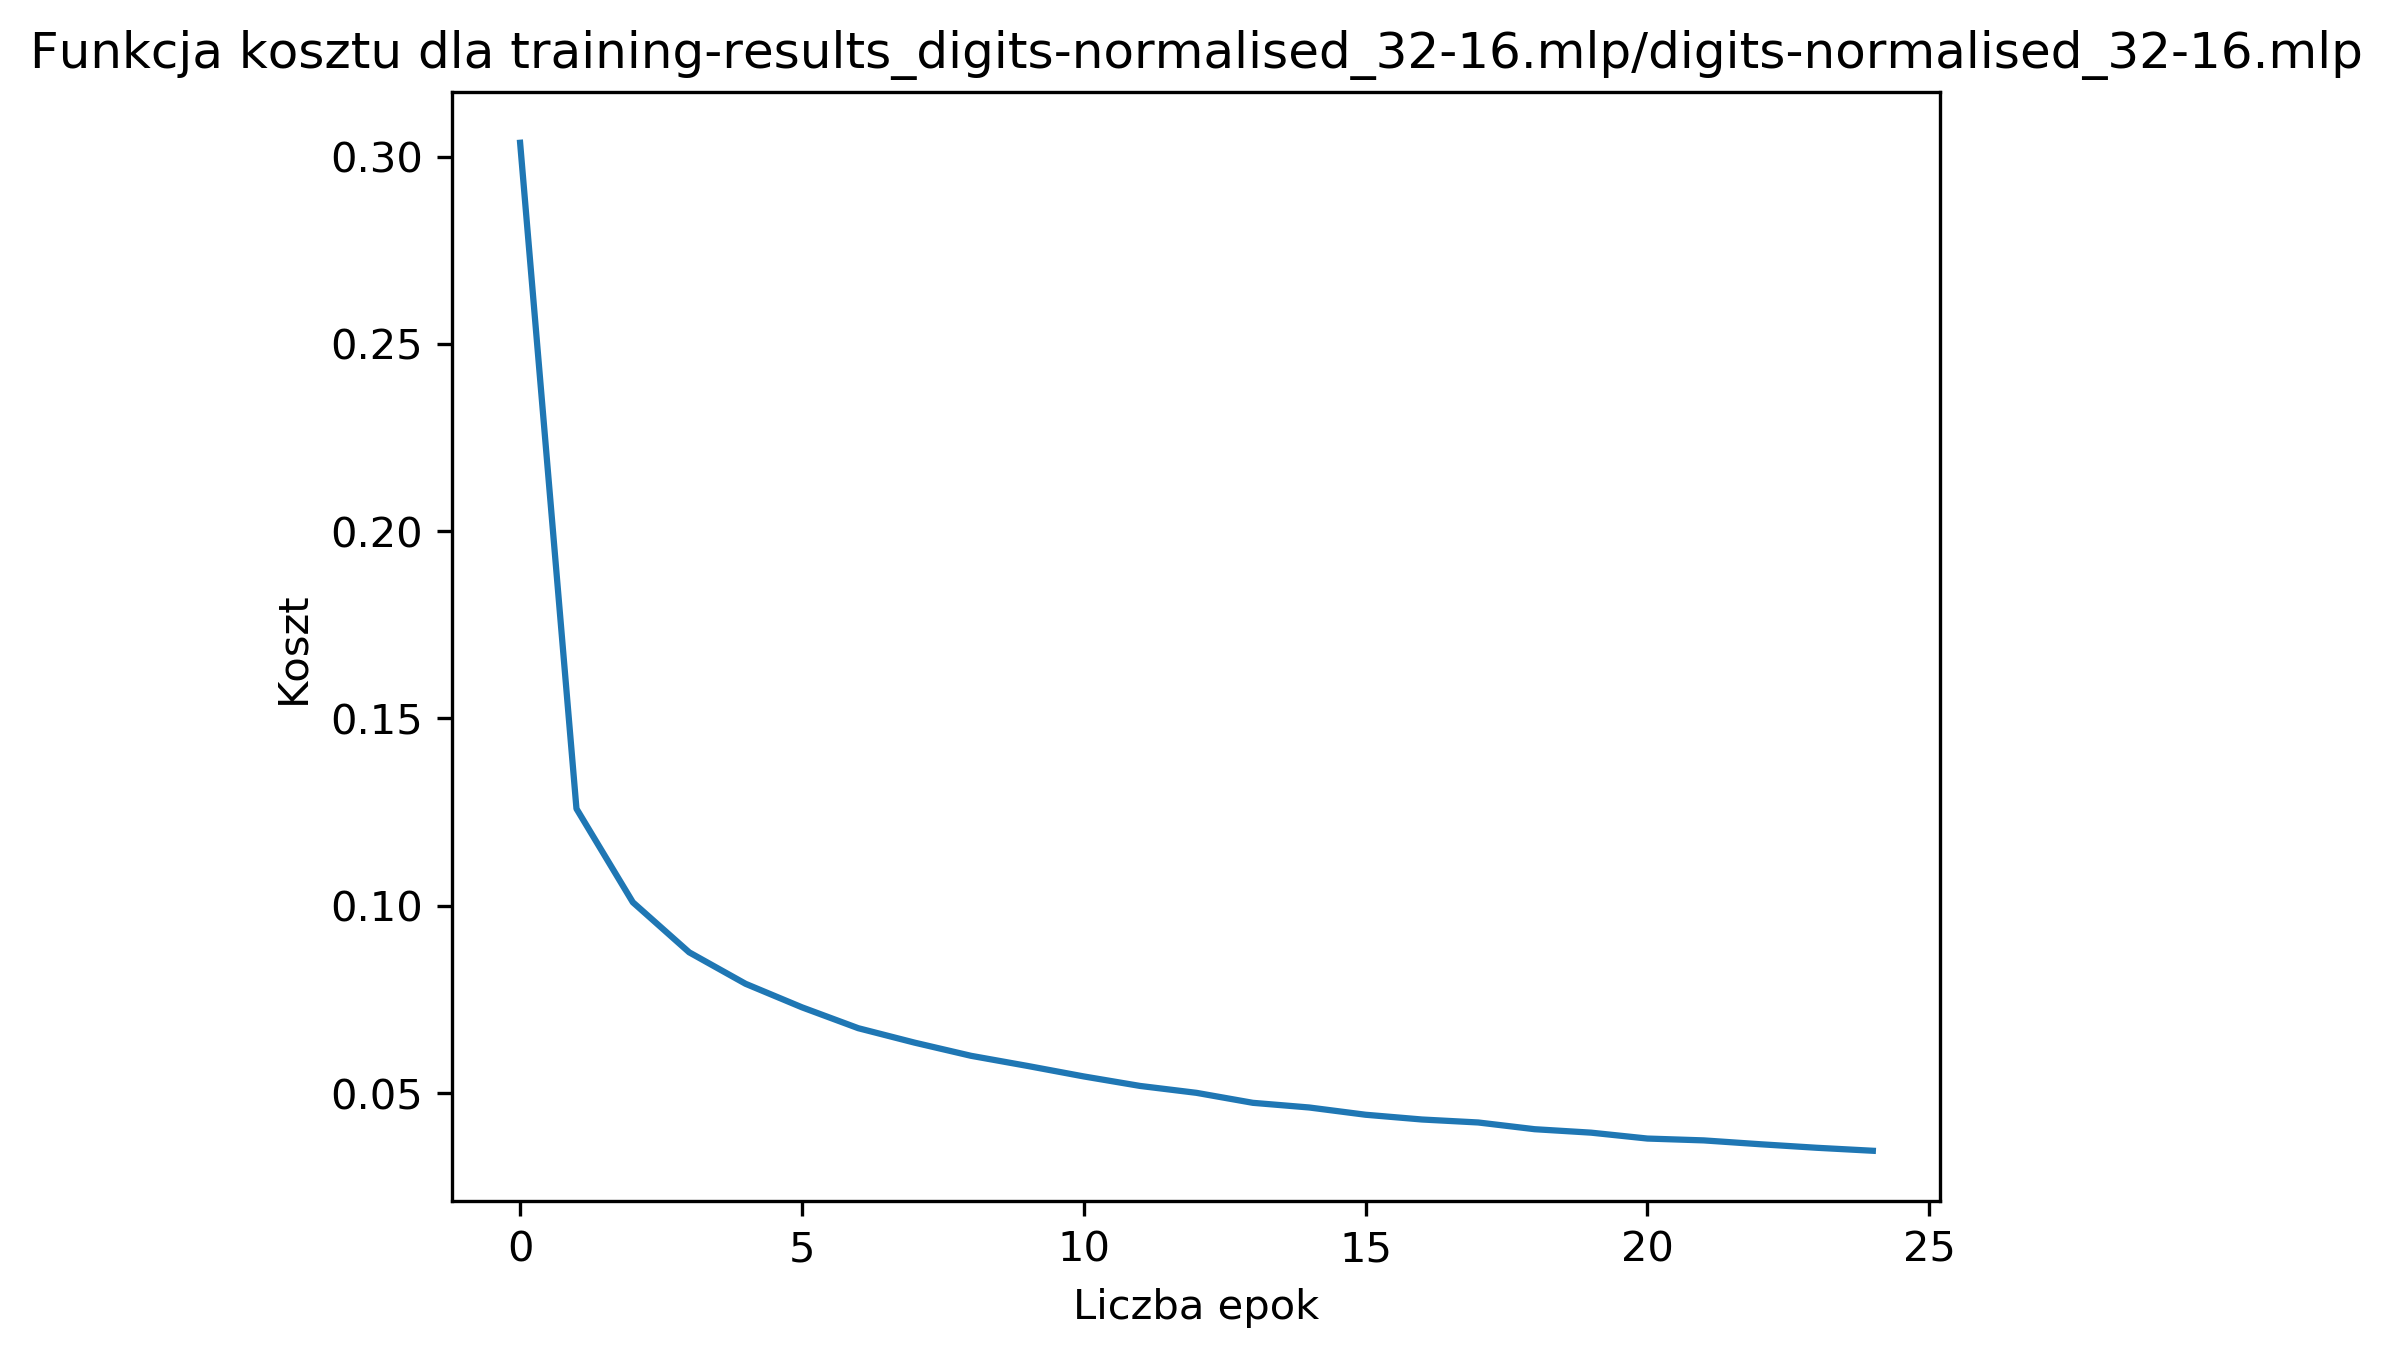
\includegraphics[width=155mm]{wykresy/digits-normalised_32-16_mlp_cost.png}
                    \caption{Tryb z standaryzowanymi danymi}
                \end{figure}
                \begin{figure}[!htbp]
                    \centering
                    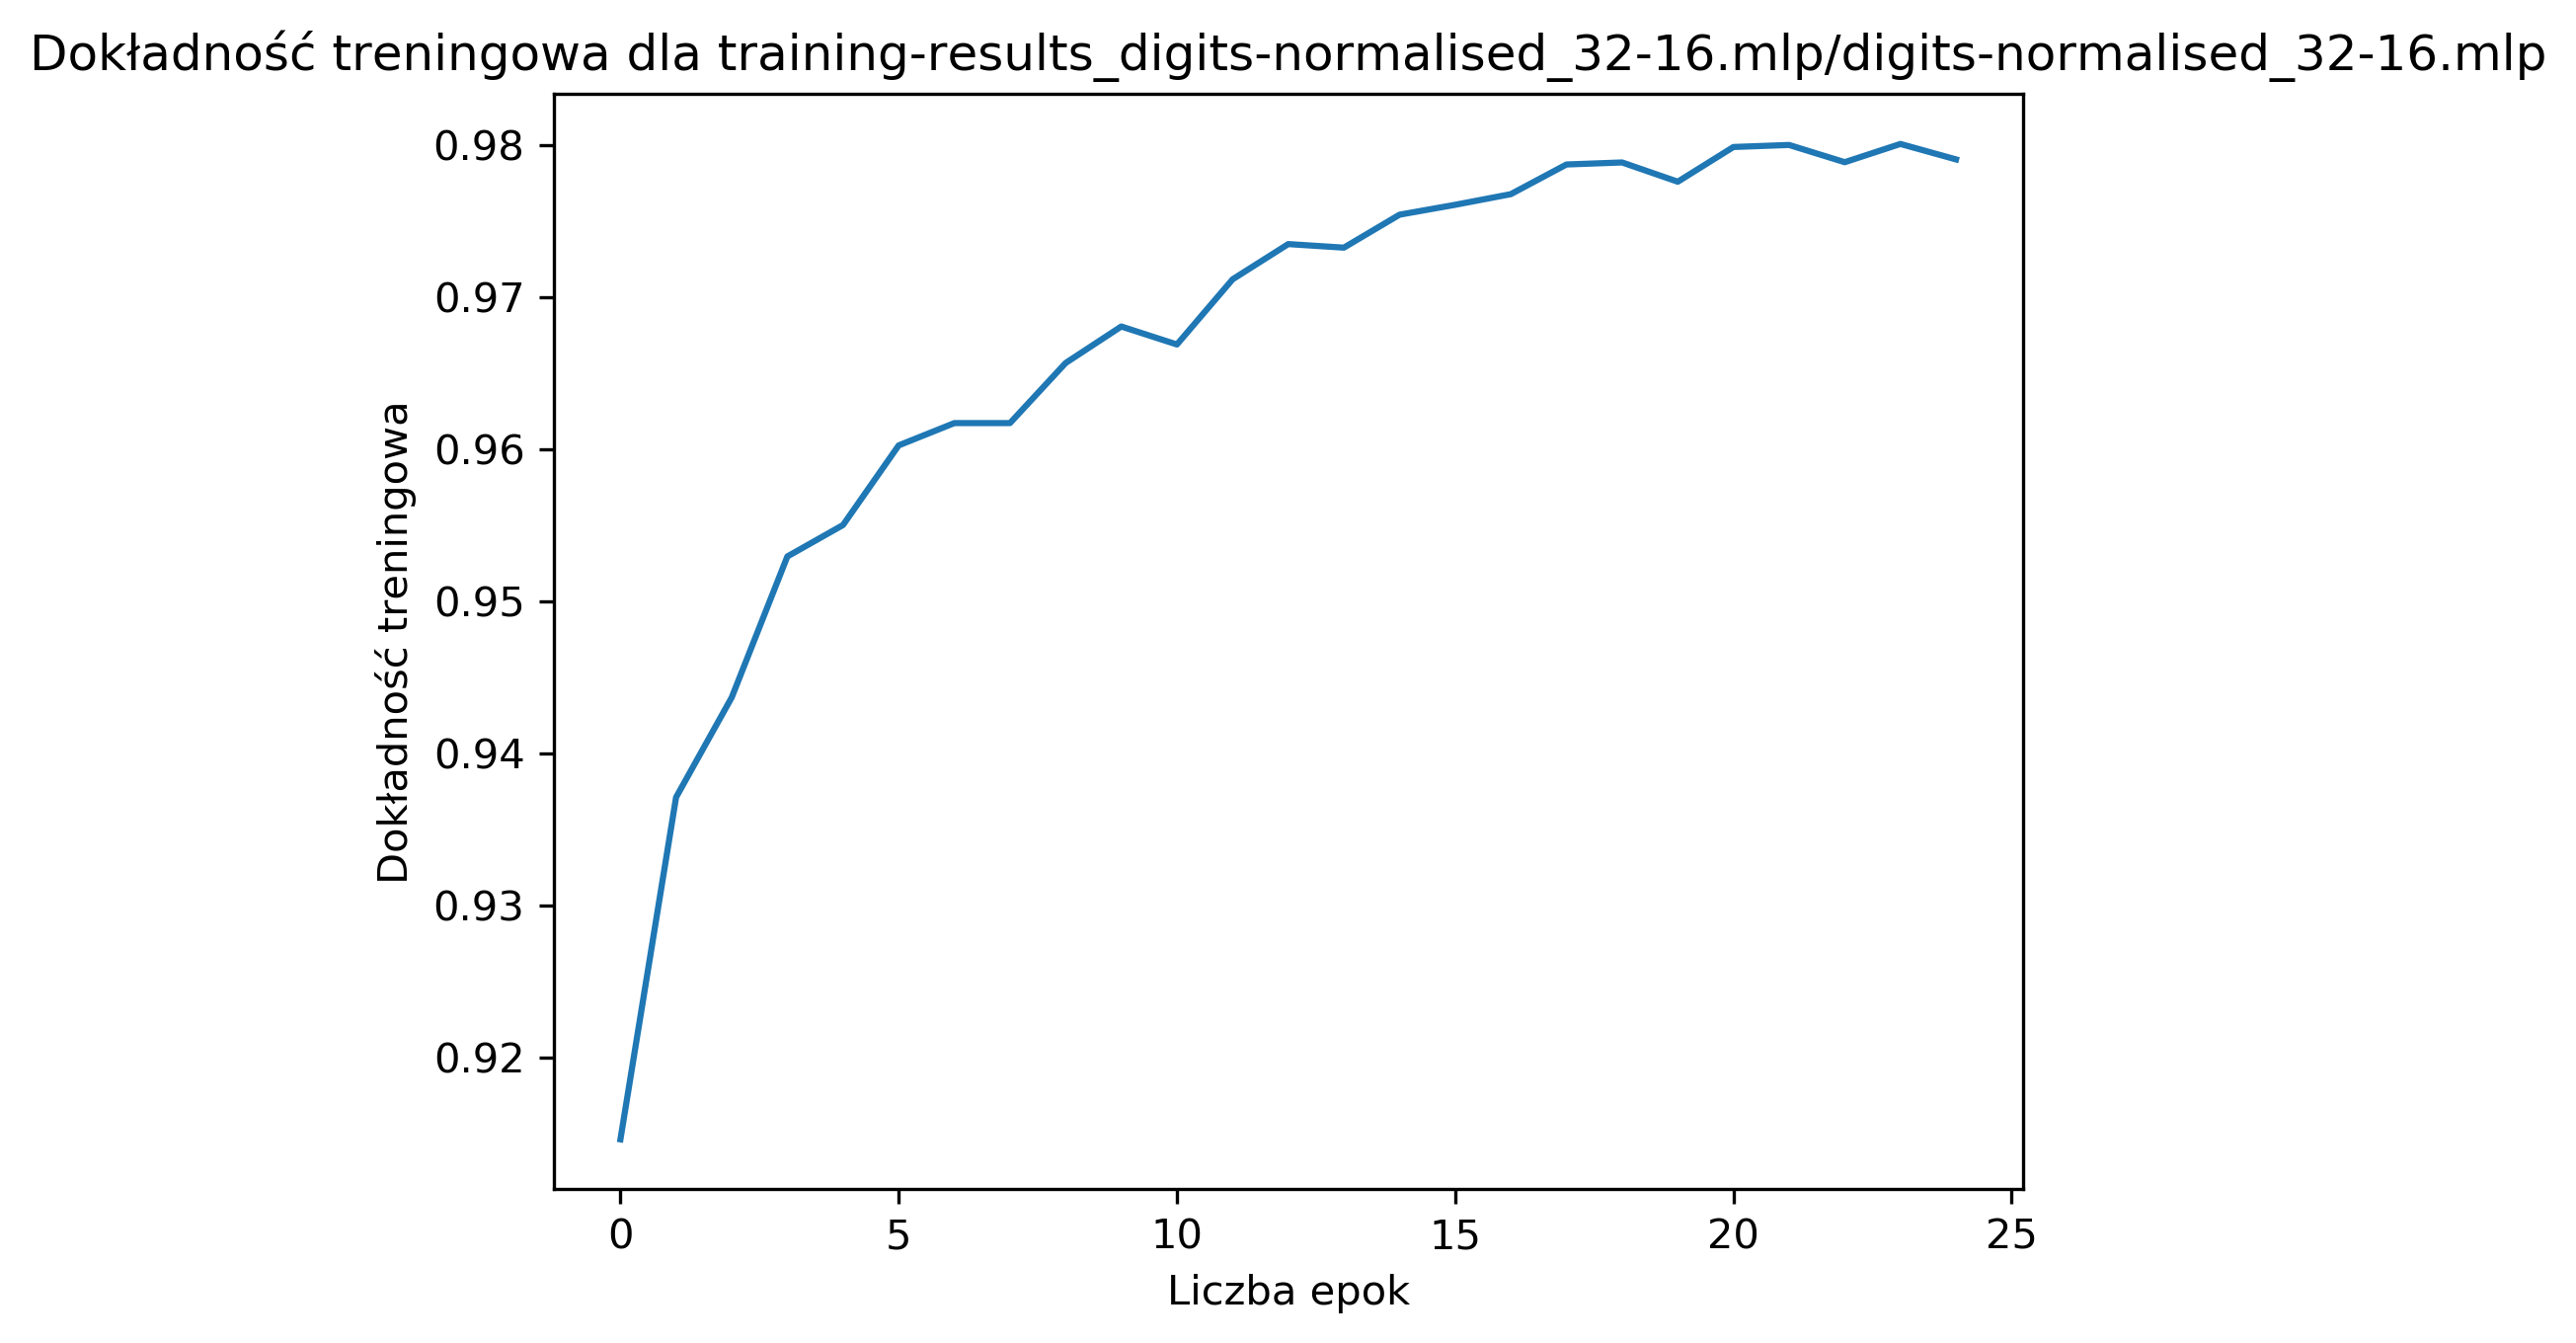
\includegraphics[width=165mm]{wykresy/digits-normalised_32-16_mlp_training-accuracy.png}
                    \caption{Tryb z standaryzowanymi danymi}
                \end{figure}
                \begin{figure}[!htbp]
                    \centering
                    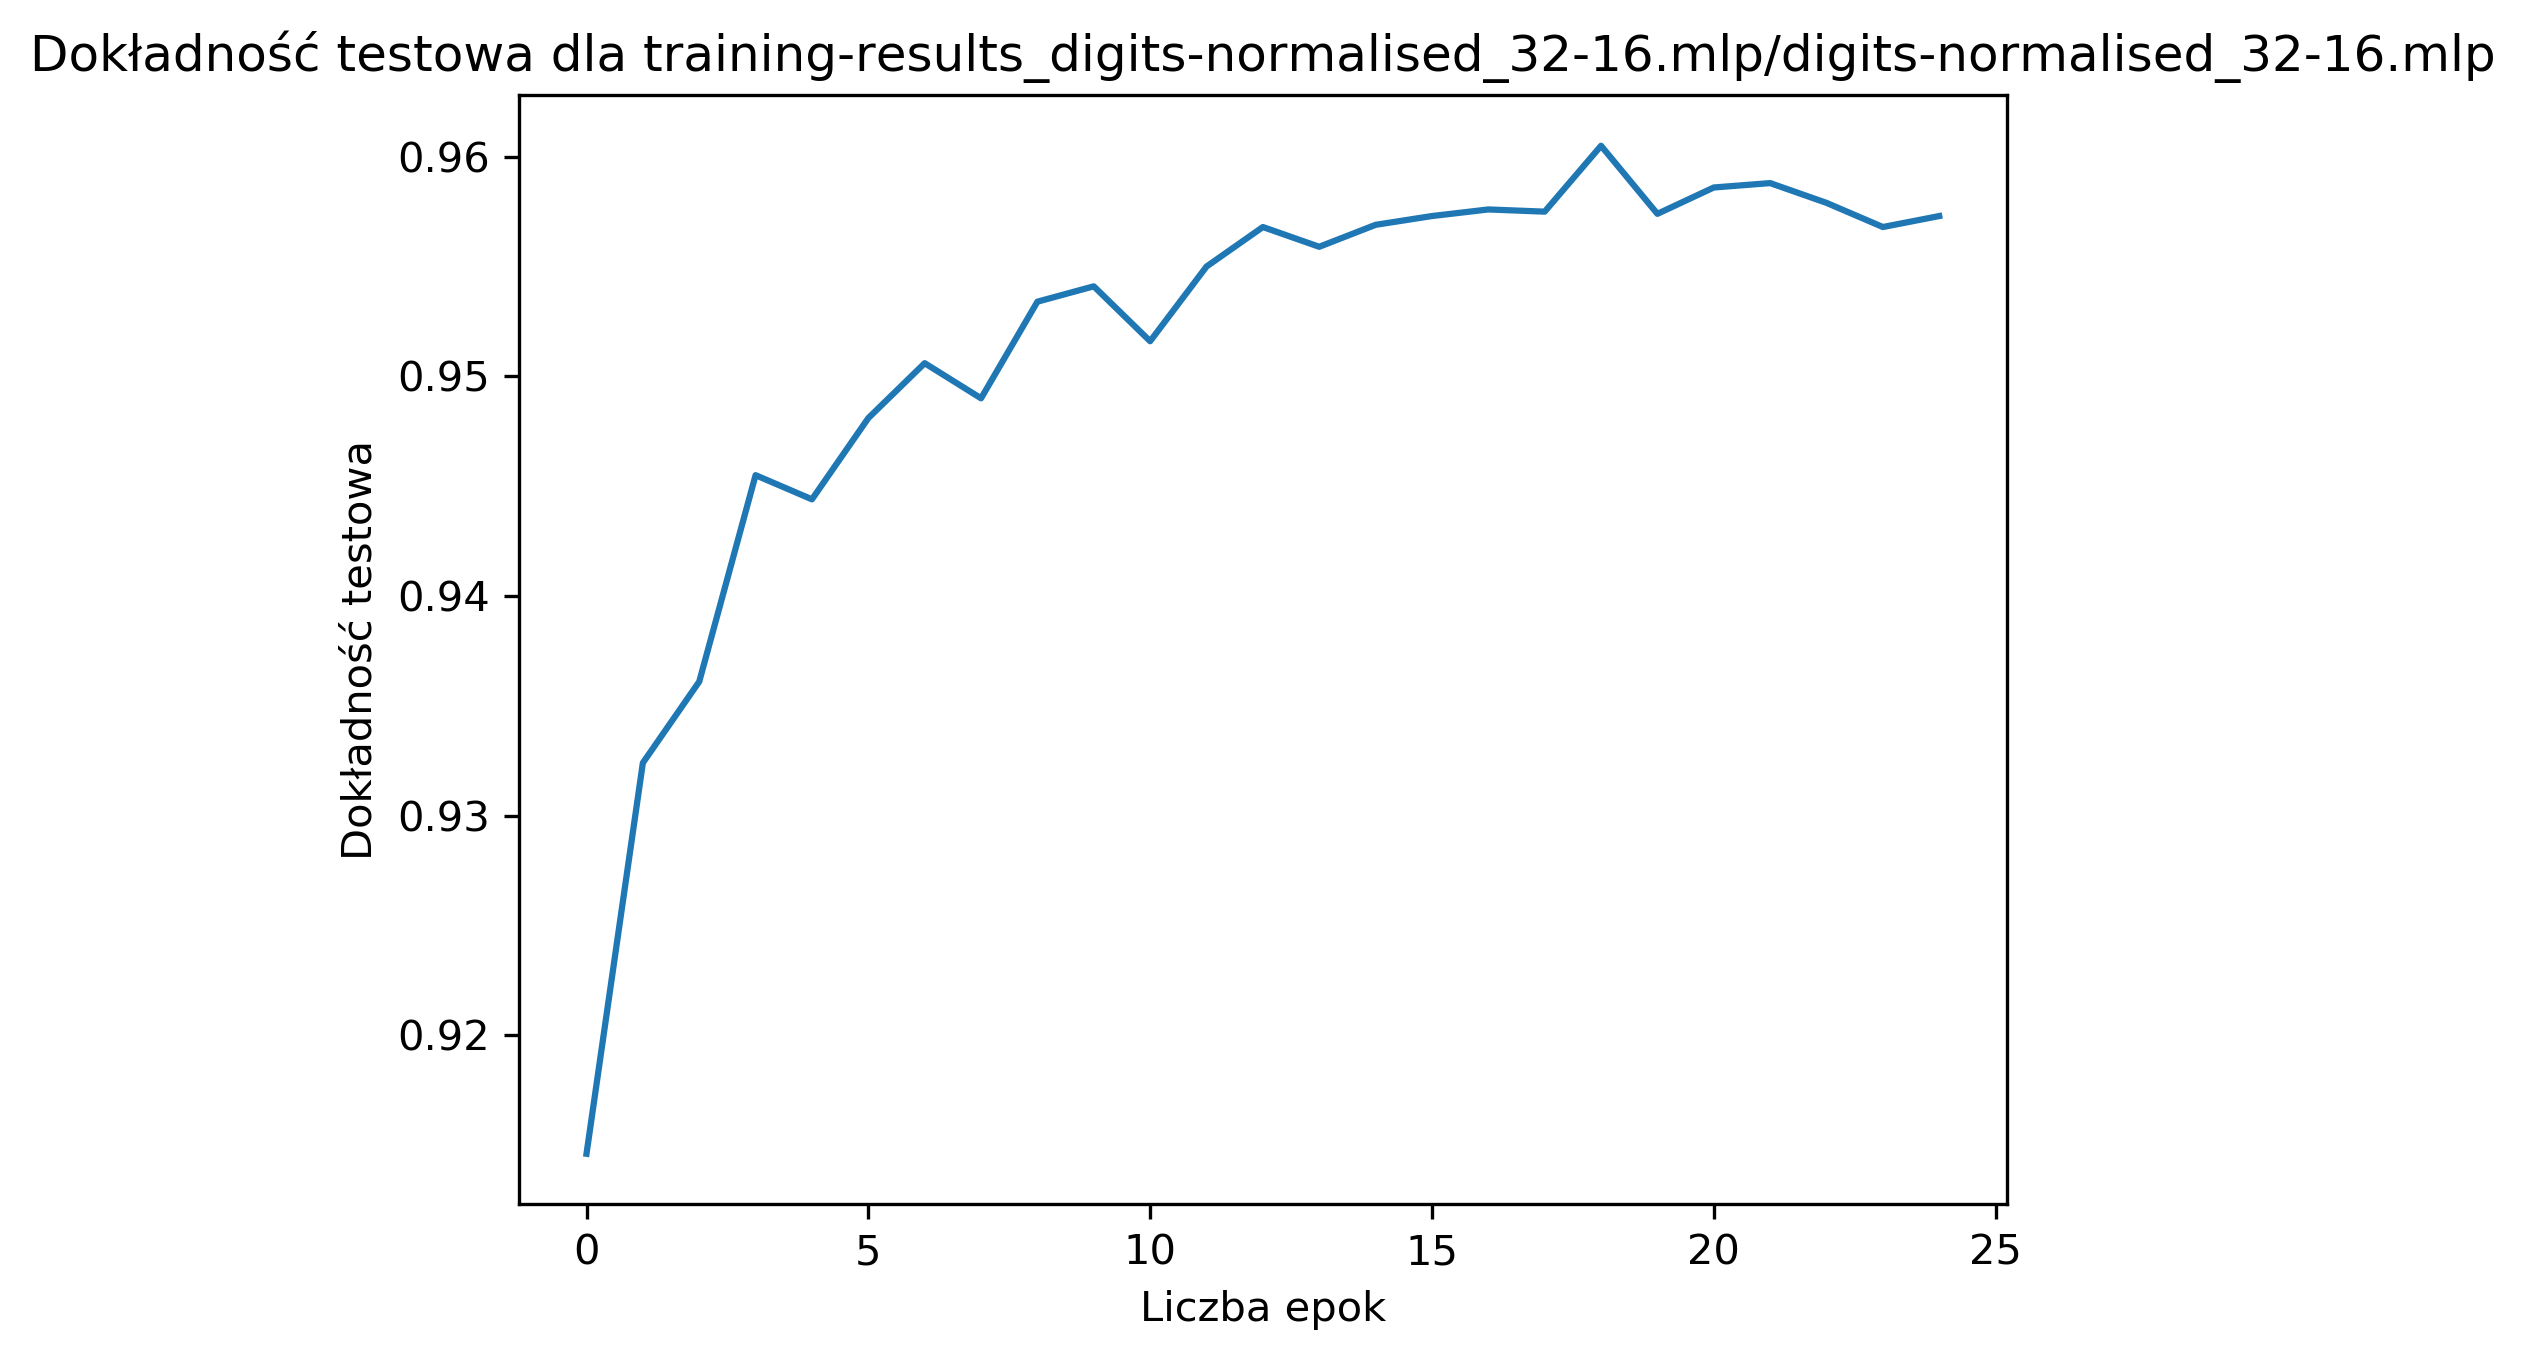
\includegraphics[width=165mm]{wykresy/digits-normalised_32-16_mlp_testing-accuracy.png}
                    \caption{Tryb z standaryzowanymi danymi}
                \end{figure}
                \FloatBarrier
            %---------------------------------------------------%
                \textbf{Dane normalizowane 128}
                \begin{figure}[!htbp]
                    \centering
                    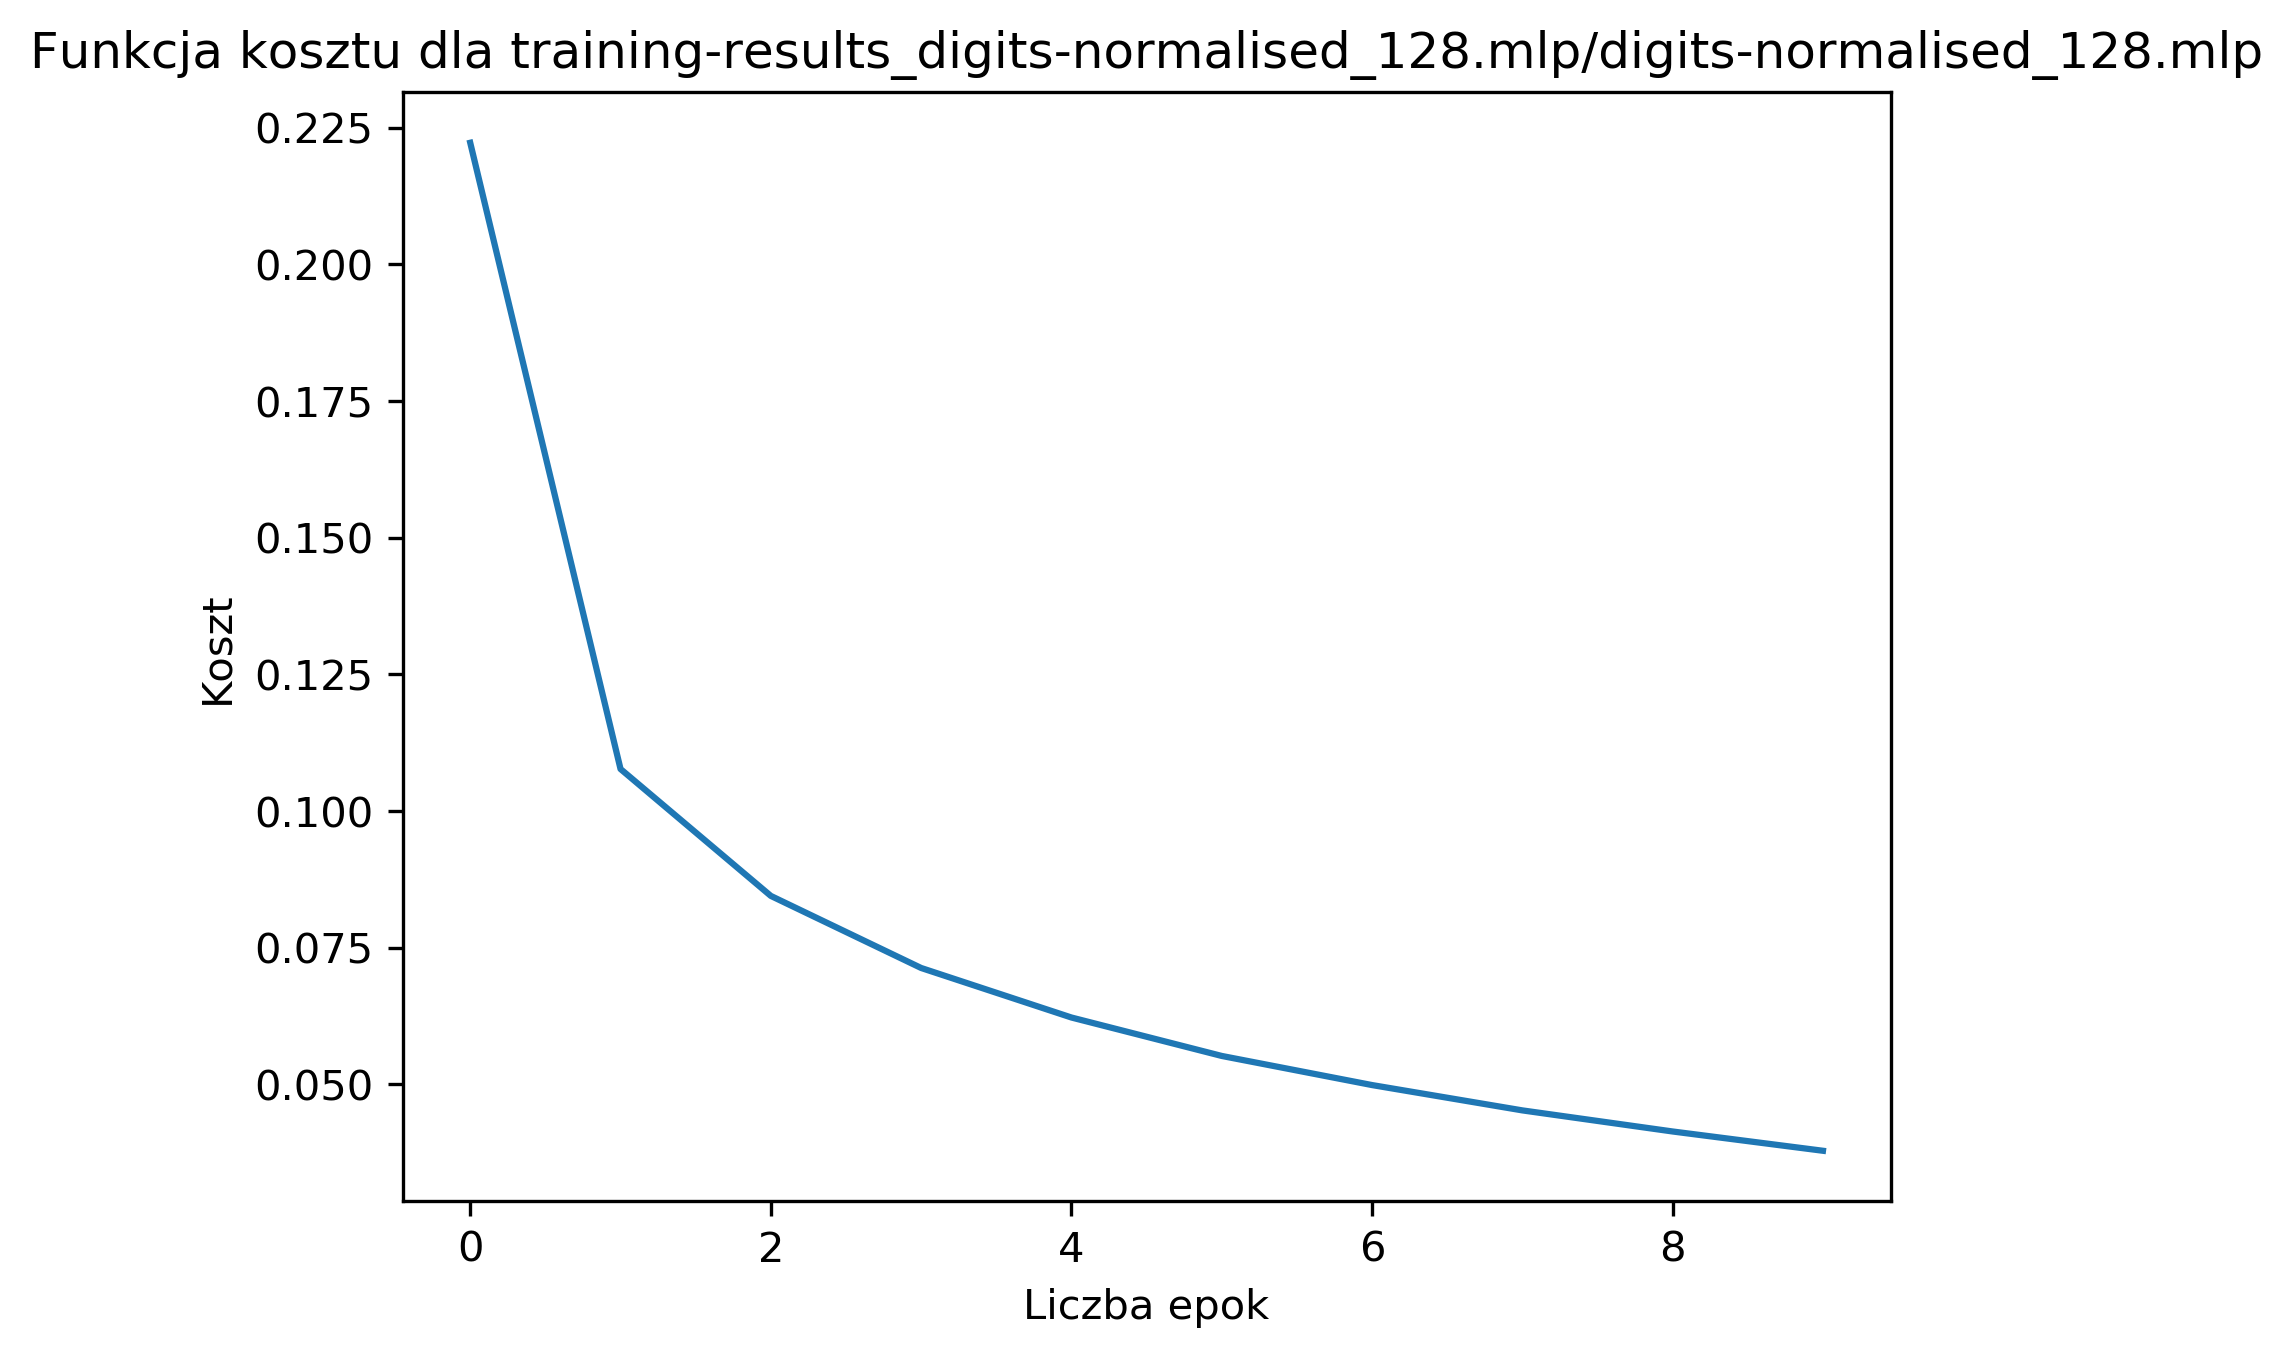
\includegraphics[width=155mm]{wykresy/digits-normalised_128_mlp_cost.png}
                    \caption{Tryb z standaryzowanymi danymi}
                \end{figure}
                \begin{figure}[!htbp]
                    \centering
                    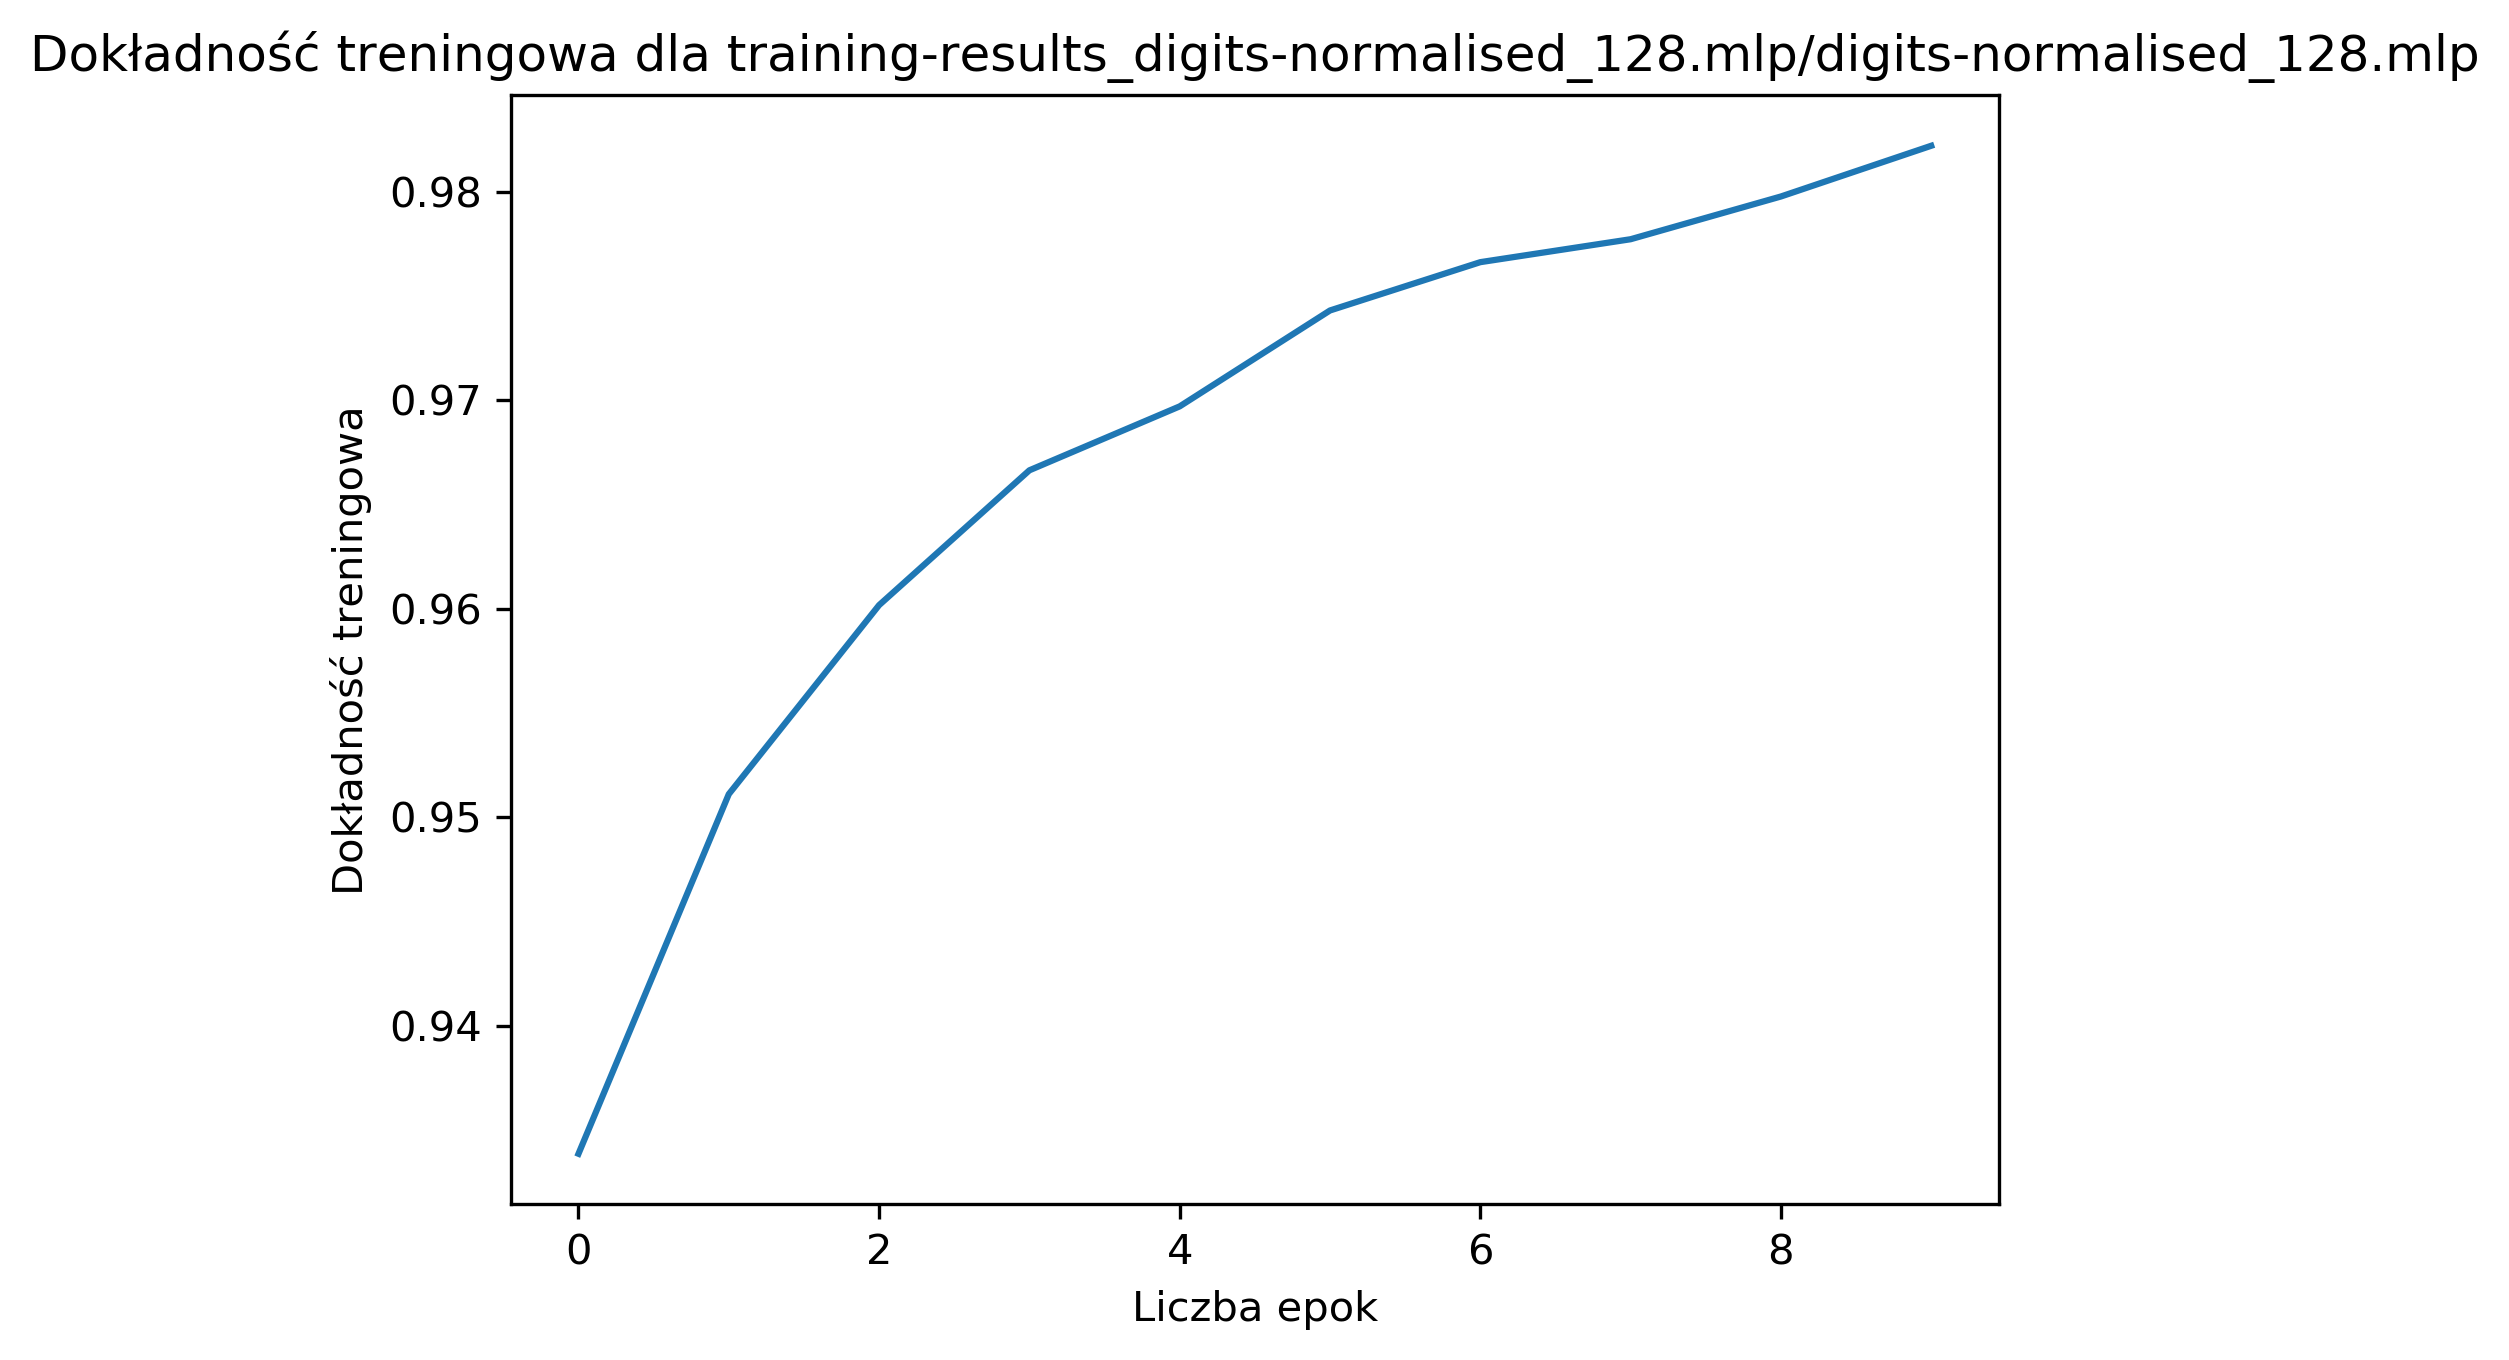
\includegraphics[width=165mm]{wykresy/digits-normalised_128_mlp_training-accuracy.png}
                    \caption{Tryb z standaryzowanymi danymi}
                \end{figure}
                \begin{figure}[!htbp]
                    \centering
                    \includegraphics[width=165mm]{wykresy/digits-normalised_128_mlp_testing-accuracy.png}
                    \caption{Tryb z standaryzowanymi danymi}
                \end{figure}
                \FloatBarrier
            %---------------------------------------------------%
            }
        %---------------------------------------------------%
            \subsubsection{K najbliższych sąsiadów}
            {
                \textbf{Tryb z domyślnymi danymi, wartość K = 5}
                \begin{lstlisting}
>> ./data/digits-test.csv

> Global confusion matrix:
                [0]    [1]   [2]   [3]   [4]   [5]   [6]   [7]   [8]  [9]
                [0] 974 0 11 0 3 5 5 0 8 5
                [1]   1 1133 8 3 7 0 3 22 3 7
                [2]   1 2 991 3 0 0 0 4 5 3
                [3]   0 0 2 976 0 12 0 0 13 9
                [4]   0 0 1 1 944 2 3 3 6 7
                [5]   1 0 0 13 0 862 2 0 12 3
                [6]   2 0 1 1 4 4 945 0 5 1
                [7]   1 0 15 6 2 1 0 988 5 10
                [8]   0 0 3 3 1 2 0 0 913 2
                [9]   0 0 0 4 21 4 0 11 4 962


                Total population | 10000

                Accuracy | 96.88 %



                > [0]
                [Positive]    [Negative]
                [Positive]          974 37
                [Negative]            6 8983


                Total population | 10000

                True positive | 974
                True negative | 8983
                False positive (type I error) | 37
                False negative (type II error) | 6

                Correct positive predictions | 96.3403 %
                Correct negative predictions | 99.9333 %

                Correct positive classifications | 99.3878 %
                Correct negative classifications | 99.5898 %

                Accuracy | 99.57 %



                > [1]
                [Positive]    [Negative]
                [Positive]         1133 54
                [Negative]            2 8811


                Total population | 10000

                True positive | 1133
                True negative | 8811
                False positive (type I error) | 54
                False negative (type II error) | 2

                Correct positive predictions | 95.4507 %
                Correct negative predictions | 99.9773 %

                Correct positive classifications | 99.8238 %
                Correct negative classifications | 99.3909 %

                Accuracy | 99.44 %



                > [2]
                [Positive]    [Negative]
                [Positive]          991 18
                [Negative]           41 8950


                Total population | 10000

                True positive | 991
                True negative | 8950
                False positive (type I error) | 18
                False negative (type II error) | 41

                Correct positive predictions | 98.2161 %
                Correct negative predictions | 99.544 %

                Correct positive classifications | 96.0271 %
                Correct negative classifications | 99.7993 %

                Accuracy | 99.41 %



                > [3]
                [Positive]    [Negative]
                [Positive]          976 36
                [Negative]           34 8954


                Total population | 10000

                True positive | 976
                True negative | 8954
                False positive (type I error) | 36
                False negative (type II error) | 34

                Correct positive predictions | 96.4427 %
                Correct negative predictions | 99.6217 %

                Correct positive classifications | 96.6337 %
                Correct negative classifications | 99.5996 %

                Accuracy | 99.3 %



                > [4]
                [Positive]    [Negative]
                [Positive]          944 23
                [Negative]           38 8995


                Total population | 10000

                True positive | 944
                True negative | 8995
                False positive (type I error) | 23
                False negative (type II error) | 38

                Correct positive predictions | 97.6215 %
                Correct negative predictions | 99.5793 %

                Correct positive classifications | 96.1303 %
                Correct negative classifications | 99.745 %

                Accuracy | 99.39 %



                > [5]
                [Positive]    [Negative]
                [Positive]          862 31
                [Negative]           30 9077


                Total population | 10000

                True positive | 862
                True negative | 9077
                False positive (type I error) | 31
                False negative (type II error) | 30

                Correct positive predictions | 96.5286 %
                Correct negative predictions | 99.6706 %

                Correct positive classifications | 96.6368 %
                Correct negative classifications | 99.6596 %

                Accuracy | 99.39 %



                > [6]
                [Positive]    [Negative]
                [Positive]          945 18
                [Negative]           13 9024


                Total population | 10000

                True positive | 945
                True negative | 9024
                False positive (type I error) | 18
                False negative (type II error) | 13

                Correct positive predictions | 98.1308 %
                Correct negative predictions | 99.8561 %

                Correct positive classifications | 98.643 %
                Correct negative classifications | 99.8009 %

                Accuracy | 99.69 %



                > [7]
                [Positive]    [Negative]
                [Positive]          988 40
                [Negative]           40 8932


                Total population | 10000

                True positive | 988
                True negative | 8932
                False positive (type I error) | 40
                False negative (type II error) | 40

                Correct positive predictions | 96.1089 %
                Correct negative predictions | 99.5542 %

                Correct positive classifications | 96.1089 %
                Correct negative classifications | 99.5542 %

                Accuracy | 99.2 %



                > [8]
                [Positive]    [Negative]
                [Positive]          913 11
                [Negative]           61 9015


                Total population | 10000

                True positive | 913
                True negative | 9015
                False positive (type I error) | 11
                False negative (type II error) | 61

                Correct positive predictions | 98.8095 %
                Correct negative predictions | 99.3279 %

                Correct positive classifications | 93.7372 %
                Correct negative classifications | 99.8781 %

                Accuracy | 99.28 %



                > [9]
                [Positive]    [Negative]
                [Positive]          962 44
                [Negative]           47 8947


                Total population | 10000

                True positive | 962
                True negative | 8947
                False positive (type I error) | 44
                False negative (type II error) | 47

                Correct positive predictions | 95.6262 %
                Correct negative predictions | 99.4774 %

                Correct positive classifications | 95.3419 %
                Correct negative classifications | 99.5106 %

                Accuracy | 99.09 %

                \end{lstlisting}
            %---------------------------------------------------%
                \textbf{Tryb HOG, wartość K = 1}
                \begin{lstlisting}
>> ./data/digits-hog-test.csv

> Global confusion matrix:
                [0]   [1]   [2]   [3]   [4]   [5]   [6]   [7]   [8]  [9]
                [0] 976 3 7 3 0 0 10 0 13 2
                [1]   2 1121 0 1 3 0 3 9 4 4
                [2]   0 3 989 5 1 0 2 7 3 0
                [3]   0 1 12 967 0 20 1 5 12 3
                [4]   0 1 2 0 932 0 1 9 3 12
                [5]   0 0 0 12 0 854 2 0 5 5
                [6]   2 2 2 0 5 9 936 0 10 0
                [7]   0 2 13 6 3 1 0 971 6 19
                [8]   0 2 3 11 3 8 3 0 908 4
                [9]   0 0 4 5 35 0 0 27 10 960


                Total population | 10000

                Accuracy | 96.14 %



                > [0]
                [Positive]    [Negative]
                [Positive]          976 38
                [Negative]            4 8982


                Total population | 10000

                True positive | 976
                True negative | 8982
                False positive (type I error) | 38
                False negative (type II error) | 4

                Correct positive predictions | 96.2525 %
                Correct negative predictions | 99.9555 %

                Correct positive classifications | 99.5918 %
                Correct negative classifications | 99.5787 %

                Accuracy | 99.58 %



                > [1]
                [Positive]    [Negative]
                [Positive]         1121 26
                [Negative]           14 8839


                Total population | 10000

                True positive | 1121
                True negative | 8839
                False positive (type I error) | 26
                False negative (type II error) | 14

                Correct positive predictions | 97.7332 %
                Correct negative predictions | 99.8419 %

                Correct positive classifications | 98.7665 %
                Correct negative classifications | 99.7067 %

                Accuracy | 99.6 %



                > [2]
                [Positive]    [Negative]
                [Positive]          989 21
                [Negative]           43 8947


                Total population | 10000

                True positive | 989
                True negative | 8947
                False positive (type I error) | 21
                False negative (type II error) | 43

                Correct positive predictions | 97.9208 %
                Correct negative predictions | 99.5217 %

                Correct positive classifications | 95.8333 %
                Correct negative classifications | 99.7658 %

                Accuracy | 99.36 %



                > [3]
                [Positive]    [Negative]
                [Positive]          967 54
                [Negative]           43 8936


                Total population | 10000

                True positive | 967
                True negative | 8936
                False positive (type I error) | 54
                False negative (type II error) | 43

                Correct positive predictions | 94.7111 %
                Correct negative predictions | 99.5211 %

                Correct positive classifications | 95.7426 %
                Correct negative classifications | 99.3993 %

                Accuracy | 99.03 %



                > [4]
                [Positive]    [Negative]
                [Positive]          932 28
                [Negative]           50 8990


                Total population | 10000

                True positive | 932
                True negative | 8990
                False positive (type I error) | 28
                False negative (type II error) | 50

                Correct positive predictions | 97.0833 %
                Correct negative predictions | 99.4469 %

                Correct positive classifications | 94.9084 %
                Correct negative classifications | 99.6895 %

                Accuracy | 99.22 %



                > [5]
                [Positive]    [Negative]
                [Positive]          854 24
                [Negative]           38 9084


                Total population | 10000

                True positive | 854
                True negative | 9084
                False positive (type I error) | 24
                False negative (type II error) | 38

                Correct positive predictions | 97.2665 %
                Correct negative predictions | 99.5834 %

                Correct positive classifications | 95.7399 %
                Correct negative classifications | 99.7365 %

                Accuracy | 99.38 %



                > [6]
                [Positive]    [Negative]
                [Positive]          936 30
                [Negative]           22 9012


                Total population | 10000

                True positive | 936
                True negative | 9012
                False positive (type I error) | 30
                False negative (type II error) | 22

                Correct positive predictions | 96.8944 %
                Correct negative predictions | 99.7565 %

                Correct positive classifications | 97.7035 %
                Correct negative classifications | 99.6682 %

                Accuracy | 99.48 %



                > [7]
                [Positive]    [Negative]
                [Positive]          971 50
                [Negative]           57 8922


                Total population | 10000

                True positive | 971
                True negative | 8922
                False positive (type I error) | 50
                False negative (type II error) | 57

                Correct positive predictions | 95.1028 %
                Correct negative predictions | 99.3652 %

                Correct positive classifications | 94.4553 %
                Correct negative classifications | 99.4427 %

                Accuracy | 98.93 %



                > [8]
                [Positive]    [Negative]
                [Positive]          908 34
                [Negative]           66 8992


                Total population | 10000

                True positive | 908
                True negative | 8992
                False positive (type I error) | 34
                False negative (type II error) | 66

                Correct positive predictions | 96.3907 %
                Correct negative predictions | 99.2714 %

                Correct positive classifications | 93.2238 %
                Correct negative classifications | 99.6233 %

                Accuracy | 99 %



                > [9]
                [Positive]    [Negative]
                [Positive]          960 81
                [Negative]           49 8910


                Total population | 10000

                True positive | 960
                True negative | 8910
                False positive (type I error) | 81
                False negative (type II error) | 49

                Correct positive predictions | 92.219 %
                Correct negative predictions | 99.4531 %

                Correct positive classifications | 95.1437 %
                Correct negative classifications | 99.0991 %

                Accuracy | 98.7 %

                \end{lstlisting}
            %---------------------------------------------------%
                \textbf{Tryb HOG, wartość K = 5}
                \begin{lstlisting}
>> ./data/digits-hog-test.csv

> Global confusion matrix:
                [0]   [1]   [2]   [3]   [4]   [5]   [6]   [7]   [8]   [9]
                [0] 975 2 9 6 0 0 7 0 16 4
                [1]  3 1123 1 0 3 0 4 7 3 5
                [2]  0 3 1003 3 1 0 0 6 3 1
                [3]  0 1 9 969 0 8 1 5 13 5
                [4]  0 0 0 1 932 0 1 6 2 6
                [5]  0 0 0 13 0 869 2 0 5 6
                [6]  1 2 1 0 6 6 943 0 9 0
                [7]  1 2 7 7 2 1 0 977 6 18
                [8]  0 2 1 8 2 8 0 1 905 4
                [9]  0 0 1 3 36 0 0 26 12 960


                Total population | 10000

                Accuracy | 96.56 %



                > [0]
                [Positive]    [Negative]
                [Positive]          975 44
                [Negative]            5 8976


                Total population | 10000

                True positive | 975
                True negative | 8976
                False positive (type I error) | 44
                False negative (type II error) | 5

                Correct positive predictions | 95.682 %
                Correct negative predictions | 99.9443 %

                Correct positive classifications | 99.4898 %
                Correct negative classifications | 99.5122 %

                Accuracy | 99.51 %



                > [1]
                [Positive]    [Negative]
                [Positive]         1123 26
                [Negative]           12 8839


                Total population | 10000

                True positive | 1123
                True negative | 8839
                False positive (type I error) | 26
                False negative (type II error) | 12

                Correct positive predictions | 97.7372 %
                Correct negative predictions | 99.8644 %

                Correct positive classifications | 98.9427 %
                Correct negative classifications | 99.7067 %

                Accuracy | 99.62 %



                > [2]
                [Positive]    [Negative]
                [Positive]         1003 17
                [Negative]           29 8951


                Total population | 10000

                True positive | 1003
                True negative | 8951
                False positive (type I error) | 17
                False negative (type II error) | 29

                Correct positive predictions | 98.3333 %
                Correct negative predictions | 99.6771 %

                Correct positive classifications | 97.1899 %
                Correct negative classifications | 99.8104 %

                Accuracy | 99.54 %



                > [3]
                [Positive]    [Negative]
                [Positive]          969 42
                [Negative]           41 8948


                Total population | 10000

                True positive | 969
                True negative | 8948
                False positive (type I error) | 42
                False negative (type II error) | 41

                Correct positive predictions | 95.8457 %
                Correct negative predictions | 99.5439 %

                Correct positive classifications | 95.9406 %
                Correct negative classifications | 99.5328 %

                Accuracy | 99.17 %



                > [4]
                [Positive]    [Negative]
                [Positive]          932 16
                [Negative]           50 9002


                Total population | 10000

                True positive | 932
                True negative | 9002
                False positive (type I error) | 16
                False negative (type II error) | 50

                Correct positive predictions | 98.3122 %
                Correct negative predictions | 99.4476 %

                Correct positive classifications | 94.9084 %
                Correct negative classifications | 99.8226 %

                Accuracy | 99.34 %



                > [5]
                [Positive]    [Negative]
                [Positive]          869 26
                [Negative]           23 9082


                Total population | 10000

                True positive | 869
                True negative | 9082
                False positive (type I error) | 26
                False negative (type II error) | 23

                Correct positive predictions | 97.095 %
                Correct negative predictions | 99.7474 %

                Correct positive classifications | 97.4215 %
                Correct negative classifications | 99.7145 %

                Accuracy | 99.51 %



                > [6]
                [Positive]    [Negative]
                [Positive]          943 25
                [Negative]           15 9017


                Total population | 10000

                True positive | 943
                True negative | 9017
                False positive (type I error) | 25
                False negative (type II error) | 15

                Correct positive predictions | 97.4174 %
                Correct negative predictions | 99.8339 %

                Correct positive classifications | 98.4342 %
                Correct negative classifications | 99.7235 %

                Accuracy | 99.6 %



                > [7]
                [Positive]    [Negative]
                [Positive]          977 44
                [Negative]           51 8928


                Total population | 10000

                True positive | 977
                True negative | 8928
                False positive (type I error) | 44
                False negative (type II error) | 51

                Correct positive predictions | 95.6905 %
                Correct negative predictions | 99.432 %

                Correct positive classifications | 95.0389 %
                Correct negative classifications | 99.5096 %

                Accuracy | 99.05 %



                > [8]
                [Positive]    [Negative]
                [Positive]          905 26
                [Negative]           69 9000


                Total population | 10000

                True positive | 905
                True negative | 9000
                False positive (type I error) | 26
                False negative (type II error) | 69

                Correct positive predictions | 97.2073 %
                Correct negative predictions | 99.2392 %

                Correct positive classifications | 92.9158 %
                Correct negative classifications | 99.7119 %

                Accuracy | 99.05 %



                > [9]
                [Positive]    [Negative]
                [Positive]          960 78
                [Negative]           49 8913


                Total population | 10000

                True positive | 960
                True negative | 8913
                False positive (type I error) | 78
                False negative (type II error) | 49

                Correct positive predictions | 92.4855 %
                Correct negative predictions | 99.4532 %

                Correct positive classifications | 95.1437 %
                Correct negative classifications | 99.1325 %

                Accuracy | 98.73 %

                \end{lstlisting}
            %---------------------------------------------------%
                \textbf{Tryb z normalizowanymi danymi, wartość K = 5}
                \begin{lstlisting}
>> ./data/digits-normalised-test.csv

> Global confusion matrix:
                [0]   [1]   [2]   [3]   [4]   [5]   [6]   [7]   [8]   [9]
                [0] 974 0 11 0 3 5 5 0 8 5
                [1]  1 1133 8 3 7 0 3 22 3 7
                [2]  1 2 991 3 0 0 0 4 5 3
                [3]  0 0 2 976 0 12 0 0 13 9
                [4]  0 0 1 1 944 2 3 3 6 7
                [5]  1 0 0 13 0 862 2 0 12 3
                [6]  2 0 1 1 4 4 945 0 5 1
                [7]  1 0 15 6 2 1 0 988 5 10
                [8]  0 0 3 3 1 2 0 0 913 2
                [9]  0 0 0 4 21 4 0 11 4 962


                Total population | 10000

                Accuracy | 96.88 %



                > [0]
                [Positive]    [Negative]
                [Positive]          974 37
                [Negative]            6 8983


                Total population | 10000

                True positive | 974
                True negative | 8983
                False positive (type I error) | 37
                False negative (type II error) | 6

                Correct positive predictions | 96.3403 %
                Correct negative predictions | 99.9333 %

                Correct positive classifications | 99.3878 %
                Correct negative classifications | 99.5898 %

                Accuracy | 99.57 %



                > [1]
                [Positive]    [Negative]
                [Positive]         1133 54
                [Negative]            2 8811


                Total population | 10000

                True positive | 1133
                True negative | 8811
                False positive (type I error) | 54
                False negative (type II error) | 2

                Correct positive predictions | 95.4507 %
                Correct negative predictions | 99.9773 %

                Correct positive classifications | 99.8238 %
                Correct negative classifications | 99.3909 %

                Accuracy | 99.44 %



                > [2]
                [Positive]    [Negative]
                [Positive]          991 18
                [Negative]           41 8950


                Total population | 10000

                True positive | 991
                True negative | 8950
                False positive (type I error) | 18
                False negative (type II error) | 41

                Correct positive predictions | 98.2161 %
                Correct negative predictions | 99.544 %

                Correct positive classifications | 96.0271 %
                Correct negative classifications | 99.7993 %

                Accuracy | 99.41 %



                > [3]
                [Positive]    [Negative]
                [Positive]          976 36
                [Negative]           34 8954


                Total population | 10000

                True positive | 976
                True negative | 8954
                False positive (type I error) | 36
                False negative (type II error) | 34

                Correct positive predictions | 96.4427 %
                Correct negative predictions | 99.6217 %

                Correct positive classifications | 96.6337 %
                Correct negative classifications | 99.5996 %

                Accuracy | 99.3 %



                > [4]
                [Positive]    [Negative]
                [Positive]          944 23
                [Negative]           38 8995


                Total population | 10000

                True positive | 944
                True negative | 8995
                False positive (type I error) | 23
                False negative (type II error) | 38

                Correct positive predictions | 97.6215 %
                Correct negative predictions | 99.5793 %

                Correct positive classifications | 96.1303 %
                Correct negative classifications | 99.745 %

                Accuracy | 99.39 %



                > [5]
                [Positive]    [Negative]
                [Positive]          862 31
                [Negative]           30 9077


                Total population | 10000

                True positive | 862
                True negative | 9077
                False positive (type I error) | 31
                False negative (type II error) | 30

                Correct positive predictions | 96.5286 %
                Correct negative predictions | 99.6706 %

                Correct positive classifications | 96.6368 %
                Correct negative classifications | 99.6596 %

                Accuracy | 99.39 %



                > [6]
                [Positive]    [Negative]
                [Positive]          945 18
                [Negative]           13 9024


                Total population | 10000

                True positive | 945
                True negative | 9024
                False positive (type I error) | 18
                False negative (type II error) | 13

                Correct positive predictions | 98.1308 %
                Correct negative predictions | 99.8561 %

                Correct positive classifications | 98.643 %
                Correct negative classifications | 99.8009 %

                Accuracy | 99.69 %



                > [7]
                [Positive]    [Negative]
                [Positive]          988 40
                [Negative]           40 8932


                Total population | 10000

                True positive | 988
                True negative | 8932
                False positive (type I error) | 40
                False negative (type II error) | 40

                Correct positive predictions | 96.1089 %
                Correct negative predictions | 99.5542 %

                Correct positive classifications | 96.1089 %
                Correct negative classifications | 99.5542 %

                Accuracy | 99.2 %



                > [8]
                [Positive]    [Negative]
                [Positive]          913 11
                [Negative]           61 9015


                Total population | 10000

                True positive | 913
                True negative | 9015
                False positive (type I error) | 11
                False negative (type II error) | 61

                Correct positive predictions | 98.8095 %
                Correct negative predictions | 99.3279 %

                Correct positive classifications | 93.7372 %
                Correct negative classifications | 99.8781 %

                Accuracy | 99.28 %



                > [9]
                [Positive]    [Negative]
                [Positive]          962 44
                [Negative]           47 8947


                Total population | 10000

                True positive | 962
                True negative | 8947
                False positive (type I error) | 44
                False negative (type II error) | 47

                Correct positive predictions | 95.6262 %
                Correct negative predictions | 99.4774 %

                Correct positive classifications | 95.3419 %
                Correct negative classifications | 99.5106 %

                Accuracy | 99.09 %

                \end{lstlisting}
            %---------------------------------------------------%
            }
        %---------------------------------------------------%
        }
    }
%--------------------------------------------------------------------------------------%
    \section{Dyskusja}
    {
        W przypadku kiedy odpowiednie wartości wejściowe mają duże róznice w zakresie (np seeds)
        obserwujemy większe skoki funkcji kosztu w czasie nauki przy czym przy tych samych parametrach
        ale kiedy zbiór jest normalizowany lub standaryzowany nauka przebiega w bardziej łagodny sposób -
        małe skoki funkcji kosztu. Do każdego zbioru należy dostosować współczynnik nauki
        przy czym kiedy bedzie zbyt mały sieć uczy się zbyt wolno lub w ogóle się nie uczy
        Przy czym kiedy bedzie za duży to aktualizacje wag są zbyt duże i przeskakują minima lokalne.
        Do wystarczającej nauki wcale nie trzeba dużej liczby epok. Zazwyczaj 100 epok jest optymalną liczbą.\\

        W metodzie K-najbiliższych sąsiadów dla zbioru irysów dane domyślne zauważyliśmy, że dla wartości nieparzystych liczby
        K wyniki ogólnej dokładności są minimalnie wyższe niż dla warstości parzystych. W ogolnej tablicy pomyłek
        można zauważyć ciekawe zjawisko, że przy stosunko dużej liczbie K = 10 zwiekszyła się liczba błednie
        zakwalifikowanych klas dla Iris-virginica. Zazwyczaj dla K z przedziału <1,5> było po jednym błędzie
        lecz w przypadku K = 10 były aż trzy błedy co jest dosyć sporym pogorszeniem. Dla danych normalizowanych
        wraz ze wzrostem wartości K działanie się poprawiało natomiast nie ma sensu zwiekszać K powyżej 5 gdyż
        wyniki dla K = 5 oraz K = 10 są praktycznie identyczne. Dla danych standartyzowanych uzyskaliśmy najlepsze
        wyniki dla wartości K = 1, w każdej z klas został popełniony jeden bład jedna ogólnie wykazało się
        to najwyższą skutecznością. Co ciekawe dla K = 3 zanotowaliśmy najmniejszą skuteczność, która kolejno wraz
        ze wzrostem K zaczeła rosnąć jednak nawet dla K = 10 zanotowaliśmy dosyć spore błedy Iris-virginica gdyż
        ich liczba wyniosła aż 3. \\

        W metodzie K-najbiliższych sąsiadów dla zbioru nasion wykonaliśmy pomiary dla K = 5. Najgorsze wyniki uzyskaliśmy
        dla domyślnego trybu danych, nie bylo to dla nas zaskoczeniem jednak sam wynik na poziomie 93\% nie można nazwać
    złym natomiast najlepszą skutecznością wykazała się próbka z danymi normalizowanymi, która w dosyć zaskakujaćy
    sposób przewyższyła dane standardyzowane. Róznića pomiedzy nimi nie była szczególnie duża bo wynosiła jeden bład
    wiecej wykonany dla danych standardyzowanych. Co ciekawe najgorsze wyniki uzyskaliśmy dla [1] gdyż w żadnym
    przypadku nie uzyskaliśmy 100\% pokrycia.\\

        W metodzie K-najbiliższych sąsiadów dla obrazów dane domyślne lub dane normalizowane nie wpłyneły w żaden sposób
        na wynik, wszelkie wartości są identyczne. Wartość K wynosiła 5. Wykonaliśmy również pomiary dla histogramu
        gradientu dla wartości K = 1 oraz K = 5, róznica procentowa ogólnej dokładności wynosiła około 0.5\% jednak
    warto zwrócić uwage na to, że w ogólnej tablicy błedy są dosyc spore różnice rzecz jasna na rzecz wartości
    K równej 5.\\

        W perceptronie wielowarstowym dla obrazów wiekszość eksperymentów jakie przeprowadzilśmy dawały wynik z zakresu
        <90\%,97\%> natomiast w jednym przypadku tzn dla danych domyślnych 128 uzyskaliśmy bardzo niską dokładność na
    poziomie 53\%. W czasie badań zauważyliśmy ogromny wpływ obróbki danych wejściowych na końcową dokładność.
    W w/w przypadku z niską skutecznością bardzo ciekawym aspektem jest to, że jedna z klas w ogółe nie została
    rozpoznana, w głownej tablicy pomyłem na przekątnej jest dosłownie zero i w kilku innnych kolumnach też jest
    pewien rozstrzał gdzie podobny efekt można byłoby uzyskać przez losowy wybór jednej z losowych cyfr.
    Najwyższą skuteczność udało nam sie uzyskać dla danych normalizowanych 128 gdzie ogólna dokładność
    wyniosła prawie 97\% a dokładność wykrycia poszczególnych liczb jest w zakresie <99\%,100\%> gdzie najmniejsza
    dokładność to 99.14\% co naszym zdaniem jest wybitnym wynikiem. Analizująć ogólną tablicą pomyłem składa się
    ona głównie z liczb na przekątniej, których wartość jest w okolicach liczby 1000 natomiast reszta liczb jest
    bliska zeru w niektórych przypadkach jest nieznacznie wyższa lecz naszym zdaniem jest to spowodowane tym,
    że część liczb jest do siebie bardzo podobna jak np 2 oraz 5. Rotacja jednej z ich o 180 stopni skutkuje tym,
    że są one prawie identyczne biorąc pod uwage odrecznę pismo a nie pismo maszynowe.
    }
%--------------------------------------------------------------------------------------%
    \section{Wnioski}
    {
        Podsumowując wykonane zadanie wnioskujemy, że:
        \begin{itemize}
            \item Mała liczba iteracji jest wystarczająca do uzyskania zadowalającą dokładności.
            \item Bledny współczynnik nauki (zbyt mały) może spowodować bardzo wolną naukę lub
            nie nauczeniem się.
            \item Dla metody najbliższych sąsiadów po przekroczeniu pewnej wartości liczby K zwiekszanie jej nie
            powoduje poprawy obliczeń. Jest to spowodowane przez uwzględnianie zbyt dużej liczby punktów.
            \item Dzieki normalizacji danych jest możliwe praktycznie jednoznaczne rozpoznanie cyfry (~99\%).
            \item W każdym przypadku dla perceptronu obróbka danych tzn normalizacja lub standardyzacja polepszała
            uzyskiwaną dokładność.
        \end{itemize}
    }
%--------------------------------------------------------------------------------------%
    \begin{thebibliography}{0}
        \bibitem{l2short}{ http://www.cs.put.poznan.pl/jstefanowski/aed/TPDANN.pdf}
        \bibitem{l2short}{mgr inż. Paweł Tarasiuk Sztuczne sieci neuronowe z propagacji w przód: przydatne
        wzory Politechnika Łódzka }
    \end{thebibliography}
%--------------------------------------------------------------------------------------%
\end{document}